%****************************************************************************************************
% main — WQU Financial Data — Module 1
% Bản dịch tiếng Việt (tài liệu học tập cá nhân)
%****************************************************************************************************
\RequirePackage{fix-cm}
\documentclass[
  oneside, titlepage, numbers=noenddot, headinclude,
  footinclude=true, cleardoublepage=empty, abstractoff,
  BCOR=5mm, paper=a4, fontsize=11pt
]{scrreprt}

%****************************************************************************************************
% classicthesis-config.tex — Writing Your Journal Article in 12 Weeks
%****************************************************************************************************

% --- Cấu hình mã hóa ký tự và phông chữ ---
\PassOptionsToPackage{utf8}{inputenc}
  \usepackage{inputenc}

\PassOptionsToPackage{T5,T1}{fontenc} % T5 cho tiếng Việt, T1 cho Palatino
  \usepackage{fontenc}
\usepackage{mathpazo} % Font Palatino cho text + math
\linespread{1.10}     % Palatino cần giãn dòng; 1.05 là mức tối thiểu, 1.10 chuẩn sách in
\usepackage{listings}

% ****************************************************************************************************
% 1. Cấu hình gói classicthesis
% ****************************************************************************************************
\PassOptionsToPackage{
  drafting=false,    
  tocaligned=false, 
  dottedtoc=false,  
  eulerchapternumbers=false, 
  floatperchapter=true,     
  eulermath=false,  
  beramono=true,    
  palatino=true,    
  style=classicthesis 
}{classicthesis}

% ****************************************************************************************************
% 2. Thông tin sách
% ****************************************************************************************************
\newcommand{\myTitle}{Viết Bài Báo Khoa Học Đăng Tạp Chí Trong 12 Tuần\xspace}
\newcommand{\mySubtitle}{Hướng dẫn thành công trong xuất bản học thuật\xspace}
\newcommand{\myDegree}{Bản dịch cá nhân\xspace}
\newcommand{\myName}{Nguyễn Văn Trung\xspace}
\newcommand{\myProf}{\xspace}
\newcommand{\myOtherProf}{\xspace}
\newcommand{\mySupervisor}{Wendy Laura Belcher\xspace}
\newcommand{\myFaculty}{\xspace}
\newcommand{\myDepartment}{\xspace}
\newcommand{\myUni}{Princeton University Press\xspace}
\newcommand{\myLocation}{Hà Nội\xspace}
\newcommand{\myTime}{2026\xspace}
\newcommand{\myVersion}{\classicthesis}

\providecommand{\mLyX}{L\kern-.1667em\lower.25em\hbox{Y}\kern-.125emX\@}

% ****************************************************************************************************
% 3. Babel cho tiếng Việt
% ****************************************************************************************************
\PassOptionsToPackage{vietnamese}{babel}
    \usepackage{babel}

\usepackage{csquotes}

% ****************************************************************************************************
% 4. Toán học
% ****************************************************************************************************
\PassOptionsToPackage{fleqn}{amsmath}       
  \usepackage{amsmath}
\usepackage{amssymb}   

% --- Fix: chữ Việt có dấu bị mất dấu khi nằm trong \text{} của công thức toán ---
% Nguyên nhân: font Palatino (mathpazo) không có glyph mã T5 (tiếng Việt).
% Cách khắc phục: ép riêng đoạn chữ Việt trong công thức dùng font T5 (vntex sẽ tự
% thay bằng font thay thế có dấu), không ảnh hưởng đến Palatino ở phần còn lại.
% Dùng: r_{\vtext{tháng}} thay vì r_{\text{tháng}}
\newcommand{\vtext}[1]{\text{\fontencoding{T5}\selectfont #1}}

% ****************************************************************************************************
% 5. Graphic & Utilities
% ****************************************************************************************************
\usepackage{graphicx} 
\usepackage{scrhack} 
\usepackage{xspace} 

% ****************************************************************************************************
% 6. Bảng & Hình
% ****************************************************************************************************
\usepackage{tabularx} 
  \setlength{\extrarowheight}{3pt} 
\newcommand{\tableheadline}[1]{\multicolumn{1}{l}{\spacedlowsmallcaps{#1}}}
\newcommand{\myfloatalign}{\centering} 
\usepackage{subfig}

% ****************************************************************************************************
% 7. TikZ & Colors
% ****************************************************************************************************
\PassOptionsToPackage{dvipsnames}{xcolor}
\usepackage{tikz}
\usetikzlibrary{positioning, fit, backgrounds, shapes.geometric}

% ****************************************************************************************************
% 8. ClassicThesis & Hyperref
% ****************************************************************************************************
\PassOptionsToPackage{hyperfootnotes=false}{hyperref}
\usepackage{classicthesis}

% Sửa lỗi chapter numbers
\usepackage{titlesec}
% Số chương: dùng \rmfamily (font thân bài mặc định, mathpazo đã trỏ về Palatino) thay vì
% \chapterNumber mặc định của classicthesis (Euler hoặc sans, không hợp phong cách "chân"
% học thuật) — cùng cách làm với dự án Black-Litterman để đồng bộ giữa các dự án.
% Muốn to/nhỏ hơn thì đổi số 100 (2 chỗ) — đơn vị pt.
\titleformat{\chapter}[display]%
  {\relax}{\mbox{}\hfill{\color{CTsemi}\fontsize{100}{100}\selectfont\rmfamily\thechapter}}{0pt}%
  {\raggedright\spacedallcaps}[\normalsize\vspace*{.8\baselineskip}\titlerule]

% Hyperref settings
\hypersetup{%
  colorlinks=true, linktocpage=true, pdfstartpage=3, pdfstartview=FitV,
  breaklinks=true, pageanchor=true,
  pdfpagemode=UseNone, 
  plainpages=false, bookmarksnumbered, bookmarksopen=true, bookmarksopenlevel=1,
  hypertexnames=true, pdfhighlight=/O,
  urlcolor=CTurl, linkcolor=CTlink, citecolor=CTcitation, 
  pdftitle={\myTitle},
  pdfauthor={\textcopyright\ \myName},
  pdfsubject={},
  pdfkeywords={},
  pdfcreator={pdfLaTeX},
  pdfproducer={LaTeX with hyperref and classicthesis}
}

% ****************************************************************************************************
% 9. Utilities
% ****************************************************************************************************
\listfiles
\usepackage{mdframed}
\mdfsetup{skipabove=6pt, skipbelow=6pt, innerleftmargin=8pt, innerrightmargin=8pt, innertopmargin=6pt, innerbottommargin=6pt}
\usepackage{tcolorbox}
\tcbset{boxrule=0.4pt, arc=0pt, left=6pt, right=6pt, top=4pt, bottom=4pt, colback=white, colframe=black}
\usepackage{multirow}
\usepackage{adjustbox}
\usepackage{booktabs}
\usepackage{float}
\floatplacement{table}{H}
\floatplacement{figure}{H}

% ****************************************************************************************************
% 10. Lề A4 (chuẩn sách 2 mặt: lề gáy > lề ngoài) + Fix URL + Xóa trang trắng thừa
% ****************************************************************************************************
% Lưu ý: dùng inner/outer thay vì left/right để lề tự đảo theo trang chẵn/lẻ khi in 2 mặt (twoside).
% Đồng thời thu hẹp khối chữ (textwidth) để còn ~62-68 ký tự/dòng theo chuẩn Bringhurst,
% tránh dòng quá dài gây cảm giác chữ "rít" khi kết hợp với line-spacing.
\usepackage[
  a4paper,
  inner=35mm,
  outer=20mm,
  top=25mm,
  bottom=30mm,
  headsep=10mm,
  twoside
]{geometry}

\PassOptionsToPackage{hyphens}{url}
\usepackage{xurl}
\setlength{\emergencystretch}{3em} % giảm bớt để tránh "sông trắng" do sloppy quá đà
% \sloppy đã bị bỏ khỏi phạm vi toàn cục — chỉ dùng cục bộ (vd. quanh URL dài) nếu cần:
% \begin{sloppypar} ... \end{sloppypar}

% Trước đây có dòng \renewcommand{\cleardoublepage}{\clearpage} để "xóa trang trắng thừa",
% nhưng làm vậy sẽ phá vỡ đồng bộ chẵn/lẻ của twoside geometry (lề gáy bị lật sai bên
% sau mỗi lần frontmatter/chương có số trang lẻ). Cách đúng: GIỮ cơ chế \cleardoublepage
% (để LaTeX tự chèn trang khi cần, đảm bảo chương luôn bắt đầu ở trang phải), nhưng thay
% nội dung trang trắng đó bằng 1 câu quote thay vì để trống — định nghĩa \cleardoublepage
% lại hoàn toàn ở bên dưới (thay cho \KOMAoptions{cleardoublepage=empty}, không cần dùng cả 2).

% --- Cơ sở dữ liệu quote (mỗi câu = 2 macro \quotetext<n> và \quoteauthor<n>) ---
% MUỐN THÊM CÂU MỚI: copy đúng 2 dòng \expandafter\def, đổi số thứ tự (tiếp theo số cuối),
% rồi tăng giá trị \nquotes bên dưới đúng bằng tổng số câu hiện có. Không cần sửa gì khác.
\makeatletter
\newcount\nquotes

\expandafter\def\csname quotetext1\endcsname{Tôi không có tài năng đặc biệt, tôi chỉ tò mò một cách say mê.}
\expandafter\def\csname quoteauthor1\endcsname{Albert Einstein}
\expandafter\def\csname quotetext2\endcsname{Trí tưởng tượng quan trọng hơn kiến thức.}
\expandafter\def\csname quoteauthor2\endcsname{Albert Einstein}
\expandafter\def\csname quotetext3\endcsname{Càng học ta càng biết mình biết ít.}
\expandafter\def\csname quoteauthor3\endcsname{Albert Einstein}
\expandafter\def\csname quotetext4\endcsname{Người không bao giờ mắc sai lầm là người không bao giờ thử điều gì mới.}
\expandafter\def\csname quoteauthor4\endcsname{Albert Einstein}
\expandafter\def\csname quotetext5\endcsname{Sự điên rồ là làm đi làm lại một việc mà vẫn mong chờ kết quả khác.}
\expandafter\def\csname quoteauthor5\endcsname{Albert Einstein}
\expandafter\def\csname quotetext6\endcsname{Cuộc sống giống như đi xe đạp, muốn giữ thăng bằng thì phải tiếp tục tiến lên.}
\expandafter\def\csname quoteauthor6\endcsname{Albert Einstein}
\expandafter\def\csname quotetext7\endcsname{Nếu tôi đã nhìn được xa hơn, ấy là vì tôi đứng trên vai những người khổng lồ.}
\expandafter\def\csname quoteauthor7\endcsname{Isaac Newton}
\expandafter\def\csname quotetext8\endcsname{Tôi có thể tính được chuyển động của các thiên thể, nhưng không thể tính được sự điên rồ của con người.}
\expandafter\def\csname quoteauthor8\endcsname{Isaac Newton}
\expandafter\def\csname quotetext9\endcsname{Chân lý luôn được tìm thấy trong sự đơn giản, chứ không phải trong sự rối rắm và hỗn loạn của vạn vật.}
\expandafter\def\csname quoteauthor9\endcsname{Isaac Newton}
\expandafter\def\csname quotetext10\endcsname{Tôi không thất bại. Tôi chỉ tìm ra mười nghìn cách không hiệu quả.}
\expandafter\def\csname quoteauthor10\endcsname{Thomas Edison}
\expandafter\def\csname quotetext11\endcsname{Thiên tài là một phần trăm cảm hứng, chín mươi chín phần trăm là mồ hôi công sức.}
\expandafter\def\csname quoteauthor11\endcsname{Thomas Edison}
\expandafter\def\csname quotetext12\endcsname{Không có gì thay thế được công việc chăm chỉ.}
\expandafter\def\csname quoteauthor12\endcsname{Thomas Edison}
\expandafter\def\csname quotetext13\endcsname{Nhiều người thất bại trong đời vì họ không nhận ra mình đã ở gần thành công đến mức nào khi từ bỏ.}
\expandafter\def\csname quoteauthor13\endcsname{Thomas Edison}
\expandafter\def\csname quotetext14\endcsname{May mắn chỉ mỉm cười với trí óc đã chuẩn bị sẵn sàng.}
\expandafter\def\csname quoteauthor14\endcsname{Louis Pasteur}
\expandafter\def\csname quotetext15\endcsname{Khoa học không có quê hương, nhưng nhà khoa học phải có quê hương.}
\expandafter\def\csname quoteauthor15\endcsname{Louis Pasteur}
\expandafter\def\csname quotetext16\endcsname{Trong lĩnh vực quan sát, cơ may chỉ ưu ái những trí óc đã được chuẩn bị.}
\expandafter\def\csname quoteauthor16\endcsname{Louis Pasteur}
\expandafter\def\csname quotetext17\endcsname{Trong đời tôi, không có gì tôi sợ, tôi chỉ tìm cách hiểu nó.}
\expandafter\def\csname quoteauthor17\endcsname{Marie Curie}
\expandafter\def\csname quotetext18\endcsname{Không có gì trong cuộc đời đáng để sợ hãi, chỉ có những điều cần được thấu hiểu.}
\expandafter\def\csname quoteauthor18\endcsname{Marie Curie}
\expandafter\def\csname quotetext19\endcsname{Con người ta không nên chú ý tới hành động của người khác, mà nên chú ý tới hành động của chính mình.}
\expandafter\def\csname quoteauthor19\endcsname{Marie Curie}
\expandafter\def\csname quotetext20\endcsname{Sự tự ti là kẻ thù lớn nhất của những giấc mơ táo bạo.}
\expandafter\def\csname quoteauthor20\endcsname{Marie Curie}
\expandafter\def\csname quotetext21\endcsname{Người dám lãng phí một giờ đồng hồ chưa hiểu hết giá trị của cuộc đời.}
\expandafter\def\csname quoteauthor21\endcsname{Charles Darwin}
\expandafter\def\csname quotetext22\endcsname{Không phải loài mạnh nhất hay thông minh nhất sống sót, mà là loài thích nghi tốt nhất với thay đổi.}
\expandafter\def\csname quoteauthor22\endcsname{Charles Darwin}
\expandafter\def\csname quotetext23\endcsname{Sự ngu dốt thường sinh ra tự tin nhiều hơn kiến thức.}
\expandafter\def\csname quoteauthor23\endcsname{Charles Darwin}
\expandafter\def\csname quotetext24\endcsname{Tôi yêu những kẻ ngu dốt biết mình ngu dốt hơn là những kẻ hiểu biết cứ tưởng mình thông thái.}
\expandafter\def\csname quoteauthor24\endcsname{Charles Darwin}
\expandafter\def\csname quotetext25\endcsname{Kiến thức nói, nhưng trí tuệ lắng nghe.}
\expandafter\def\csname quoteauthor25\endcsname{Jimi Hendrix}
\expandafter\def\csname quotetext26\endcsname{Tôi tư duy nên tôi tồn tại.}
\expandafter\def\csname quoteauthor26\endcsname{René Descartes}
\expandafter\def\csname quotetext27\endcsname{Điều duy nhất tôi biết chắc là tôi chẳng biết gì cả.}
\expandafter\def\csname quoteauthor27\endcsname{Socrates}
\expandafter\def\csname quotetext28\endcsname{Cuộc đời không được kiểm nghiệm thì không đáng sống.}
\expandafter\def\csname quoteauthor28\endcsname{Socrates}
\expandafter\def\csname quotetext29\endcsname{Biết mình không biết gì cũng đã là một loại tri thức.}
\expandafter\def\csname quoteauthor29\endcsname{Socrates}
\expandafter\def\csname quotetext30\endcsname{Giáo dục là thắp lên một ngọn lửa, chứ không phải đổ đầy một cái bình.}
\expandafter\def\csname quoteauthor30\endcsname{Socrates}
\expandafter\def\csname quotetext31\endcsname{Trí tuệ bắt đầu từ sự ngạc nhiên.}
\expandafter\def\csname quoteauthor31\endcsname{Socrates}
\expandafter\def\csname quotetext32\endcsname{Người thông thái nhất biết rằng mình không biết gì.}
\expandafter\def\csname quoteauthor32\endcsname{Plato}
\expandafter\def\csname quotetext33\endcsname{Sự thiếu hiểu biết là gốc rễ của mọi tội ác.}
\expandafter\def\csname quoteauthor33\endcsname{Plato}
\expandafter\def\csname quotetext34\endcsname{Có thể tha thứ cho một đứa trẻ sợ bóng tối, bi kịch thực sự là khi người lớn sợ ánh sáng.}
\expandafter\def\csname quoteauthor34\endcsname{Plato}
\expandafter\def\csname quotetext35\endcsname{Chúng ta là những gì ta lặp đi lặp lại. Xuất sắc, vì thế, không phải là hành động, mà là thói quen.}
\expandafter\def\csname quoteauthor35\endcsname{Aristotle}
\expandafter\def\csname quotetext36\endcsname{Giáo dục có gốc rễ đắng cay, nhưng quả của nó lại ngọt ngào.}
\expandafter\def\csname quoteauthor36\endcsname{Aristotle}
\expandafter\def\csname quotetext37\endcsname{Người có học khác người vô học cũng như người sống khác kẻ đã chết.}
\expandafter\def\csname quoteauthor37\endcsname{Aristotle}
\expandafter\def\csname quotetext38\endcsname{Kẻ mạnh không phải kẻ chiến thắng người khác, mà là kẻ chiến thắng chính mình.}
\expandafter\def\csname quoteauthor38\endcsname{Aristotle}
\expandafter\def\csname quotetext39\endcsname{Không có gì vĩ đại được tạo ra một cách vội vàng.}
\expandafter\def\csname quoteauthor39\endcsname{Epictetus}
\expandafter\def\csname quotetext40\endcsname{Chúng ta không thể lựa chọn hoàn cảnh, nhưng luôn có thể lựa chọn cách phản ứng với nó.}
\expandafter\def\csname quoteauthor40\endcsname{Epictetus}
\expandafter\def\csname quotetext41\endcsname{Trước tiên hãy nói với bản thân mình muốn trở thành người như thế nào, rồi làm những gì bạn phải làm.}
\expandafter\def\csname quoteauthor41\endcsname{Epictetus}
\expandafter\def\csname quotetext42\endcsname{Người không hài lòng với những gì mình có, sẽ không bao giờ hài lòng với những gì mình muốn có.}
\expandafter\def\csname quoteauthor42\endcsname{Socrates}
\expandafter\def\csname quotetext43\endcsname{Tri thức là sức mạnh.}
\expandafter\def\csname quoteauthor43\endcsname{Francis Bacon}
\expandafter\def\csname quotetext44\endcsname{Đọc sách không phải để phản bác hay tin ngay, mà để cân nhắc và suy xét.}
\expandafter\def\csname quoteauthor44\endcsname{Francis Bacon}
\expandafter\def\csname quotetext45\endcsname{Người khôn ngoan tạo ra nhiều cơ hội hơn là tìm thấy chúng.}
\expandafter\def\csname quoteauthor45\endcsname{Francis Bacon}
\expandafter\def\csname quotetext46\endcsname{Người dịch sách giỏi là người phản bội trung thành nhất với nguyên tác.}
\expandafter\def\csname quoteauthor46\endcsname{Khuyết danh}
\expandafter\def\csname quotetext47\endcsname{Người thầy trung bình chỉ biết nói. Người thầy giỏi biết giải thích. Người thầy xuất sắc biết minh họa. Người thầy vĩ đại biết truyền cảm hứng.}
\expandafter\def\csname quoteauthor47\endcsname{William Arthur Ward}
\expandafter\def\csname quotetext48\endcsname{Bản thảo đầu tiên nào cũng dở, kể cả của những nhà văn giỏi nhất.}
\expandafter\def\csname quoteauthor48\endcsname{Anne Lamott}
\expandafter\def\csname quotetext49\endcsname{Tôi viết để tìm hiểu xem mình nghĩ gì.}
\expandafter\def\csname quoteauthor49\endcsname{Joan Didion}
\expandafter\def\csname quotetext50\endcsname{Không có nhà văn nào giỏi ngay từ bản thảo đầu tiên.}
\expandafter\def\csname quoteauthor50\endcsname{Ernest Hemingway}
\expandafter\def\csname quotetext51\endcsname{Viết dễ thôi: bạn chỉ cần ngồi trước trang giấy trắng cho đến khi trán rịn mồ hôi.}
\expandafter\def\csname quoteauthor51\endcsname{Ernest Hemingway}
\expandafter\def\csname quotetext52\endcsname{Hãy viết say sưa, biên tập tỉnh táo.}
\expandafter\def\csname quoteauthor52\endcsname{Ernest Hemingway}
\expandafter\def\csname quotetext53\endcsname{Người viết văn hay không phải người có nhiều chữ, mà là người biết bỏ bớt chữ thừa.}
\expandafter\def\csname quoteauthor53\endcsname{Khuyết danh}
\expandafter\def\csname quotetext54\endcsname{Sự đơn giản là đỉnh cao của tinh tế.}
\expandafter\def\csname quoteauthor54\endcsname{Leonardo da Vinci}
\expandafter\def\csname quotetext55\endcsname{Học không bao giờ làm cạn kiệt trí óc.}
\expandafter\def\csname quoteauthor55\endcsname{Leonardo da Vinci}
\expandafter\def\csname quotetext56\endcsname{Sự thông thái là con gái của kinh nghiệm.}
\expandafter\def\csname quoteauthor56\endcsname{Leonardo da Vinci}
\expandafter\def\csname quotetext57\endcsname{Kẻ yêu thực hành mà không có lý thuyết giống như thủy thủ lên tàu không có la bàn.}
\expandafter\def\csname quoteauthor57\endcsname{Leonardo da Vinci}
\expandafter\def\csname quotetext58\endcsname{Nghệ thuật không bao giờ hoàn thành, chỉ bị bỏ dở.}
\expandafter\def\csname quoteauthor58\endcsname{Leonardo da Vinci}
\expandafter\def\csname quotetext59\endcsname{Giáo dục là vũ khí mạnh nhất để thay đổi thế giới.}
\expandafter\def\csname quoteauthor59\endcsname{Nelson Mandela}
\expandafter\def\csname quotetext60\endcsname{Điều tưởng chừng bất khả thi luôn là bất khả thi cho đến khi nó được thực hiện.}
\expandafter\def\csname quoteauthor60\endcsname{Nelson Mandela}
\expandafter\def\csname quotetext61\endcsname{Tôi không bao giờ thua, tôi chỉ thắng hoặc học được điều gì đó.}
\expandafter\def\csname quoteauthor61\endcsname{Nelson Mandela}
\expandafter\def\csname quotetext62\endcsname{Can đảm không phải là không sợ hãi, mà là chiến thắng nỗi sợ hãi đó.}
\expandafter\def\csname quoteauthor62\endcsname{Nelson Mandela}
\expandafter\def\csname quotetext63\endcsname{Bóng tối không thể xua tan bóng tối, chỉ ánh sáng mới làm được điều đó.}
\expandafter\def\csname quoteauthor63\endcsname{Martin Luther King Jr.}
\expandafter\def\csname quotetext64\endcsname{Thước đo cuối cùng của một con người không phải ở chỗ họ đứng đâu lúc thuận lợi, mà ở chỗ họ đứng đâu lúc khó khăn.}
\expandafter\def\csname quoteauthor64\endcsname{Martin Luther King Jr.}
\expandafter\def\csname quotetext65\endcsname{Cách tốt nhất để dự đoán tương lai là tự mình tạo ra nó.}
\expandafter\def\csname quoteauthor65\endcsname{Abraham Lincoln}
\expandafter\def\csname quotetext66\endcsname{Cho tôi sáu giờ để chặt một cái cây, tôi sẽ dùng bốn giờ đầu để mài rìu.}
\expandafter\def\csname quoteauthor66\endcsname{Abraham Lincoln}
\expandafter\def\csname quotetext67\endcsname{Thành công không phải là đích đến, thất bại không phải là điểm kết, chỉ có lòng can đảm để tiếp tục mới đáng kể.}
\expandafter\def\csname quoteauthor67\endcsname{Winston Churchill}
\expandafter\def\csname quotetext68\endcsname{Chúng ta uốn nắn các tòa nhà của mình, rồi sau đó các tòa nhà uốn nắn lại chúng ta.}
\expandafter\def\csname quoteauthor68\endcsname{Winston Churchill}
\expandafter\def\csname quotetext69\endcsname{Không bao giờ, không bao giờ, không bao giờ từ bỏ.}
\expandafter\def\csname quoteauthor69\endcsname{Winston Churchill}
\expandafter\def\csname quotetext70\endcsname{Sự dũng cảm là điều kiện đầu tiên vì nó bảo đảm cho tất cả những đức tính khác.}
\expandafter\def\csname quoteauthor70\endcsname{Winston Churchill}
\expandafter\def\csname quotetext71\endcsname{Hãy là sự thay đổi mà bạn muốn thấy trên thế giới.}
\expandafter\def\csname quoteauthor71\endcsname{Mahatma Gandhi}
\expandafter\def\csname quotetext72\endcsname{Sống như thể ngày mai bạn sẽ chết, học như thể bạn sẽ sống mãi mãi.}
\expandafter\def\csname quoteauthor72\endcsname{Mahatma Gandhi}
\expandafter\def\csname quotetext73\endcsname{Sức mạnh không đến từ khả năng thể chất, mà đến từ ý chí bất khuất.}
\expandafter\def\csname quoteauthor73\endcsname{Mahatma Gandhi}
\expandafter\def\csname quotetext74\endcsname{Hạnh phúc là khi những gì bạn nghĩ, những gì bạn nói và những gì bạn làm hòa hợp với nhau.}
\expandafter\def\csname quoteauthor74\endcsname{Mahatma Gandhi}
\expandafter\def\csname quotetext75\endcsname{Không ai tắm hai lần trên cùng một dòng sông.}
\expandafter\def\csname quoteauthor75\endcsname{Heraclitus}
\expandafter\def\csname quotetext76\endcsname{Sự thay đổi là điều duy nhất không đổi.}
\expandafter\def\csname quoteauthor76\endcsname{Heraclitus}
\expandafter\def\csname quotetext77\endcsname{Tính cách của một người chính là số phận của người đó.}
\expandafter\def\csname quoteauthor77\endcsname{Heraclitus}
\expandafter\def\csname quotetext78\endcsname{Đời người ngắn ngủi, nghệ thuật thì dài lâu.}
\expandafter\def\csname quoteauthor78\endcsname{Hippocrates}
\expandafter\def\csname quotetext79\endcsname{Trước hết, đừng gây hại.}
\expandafter\def\csname quoteauthor79\endcsname{Hippocrates}
\expandafter\def\csname quotetext80\endcsname{Hãy để thức ăn là thuốc của bạn, và thuốc là thức ăn của bạn.}
\expandafter\def\csname quoteauthor80\endcsname{Hippocrates}
\expandafter\def\csname quotetext81\endcsname{Người dám bắt đầu đã đi được nửa chặng đường.}
\expandafter\def\csname quoteauthor81\endcsname{Horace}
\expandafter\def\csname quotetext82\endcsname{Hãy nắm lấy ngày hôm nay, đừng đặt niềm tin vào ngày mai.}
\expandafter\def\csname quoteauthor82\endcsname{Horace}
\expandafter\def\csname quotetext83\endcsname{Ai không học được từ lịch sử sẽ buộc phải lặp lại nó.}
\expandafter\def\csname quoteauthor83\endcsname{George Santayana}
\expandafter\def\csname quotetext84\endcsname{Không có gió thuận cho con thuyền không biết mình sẽ đi về đâu.}
\expandafter\def\csname quoteauthor84\endcsname{Seneca}
\expandafter\def\csname quotetext85\endcsname{Chúng ta khổ đau nhiều hơn trong tưởng tượng so với thực tế.}
\expandafter\def\csname quoteauthor85\endcsname{Seneca}
\expandafter\def\csname quotetext86\endcsname{Toàn bộ tương lai nằm trong sự kiên nhẫn.}
\expandafter\def\csname quoteauthor86\endcsname{Seneca}
\expandafter\def\csname quotetext87\endcsname{Cuộc sống đủ dài nếu bạn biết cách sử dụng nó.}
\expandafter\def\csname quoteauthor87\endcsname{Seneca}
\expandafter\def\csname quotetext88\endcsname{Sự chờ đợi luôn tệ hơn nỗi đau thực sự.}
\expandafter\def\csname quoteauthor88\endcsname{Seneca}
\expandafter\def\csname quotetext89\endcsname{Tất cả mọi tàn ác đều bắt nguồn từ sự yếu đuối.}
\expandafter\def\csname quoteauthor89\endcsname{Seneca}
\expandafter\def\csname quotetext90\endcsname{Người khôn ngoan sống trong hiện tại, tận hưởng mọi khoảnh khắc trong yên bình.}
\expandafter\def\csname quoteauthor90\endcsname{Marcus Aurelius}
\expandafter\def\csname quotetext91\endcsname{Bạn có quyền lực đối với tâm trí mình, không phải với các sự kiện bên ngoài, hãy nhận ra điều này và bạn sẽ tìm thấy sức mạnh.}
\expandafter\def\csname quoteauthor91\endcsname{Marcus Aurelius}
\expandafter\def\csname quotetext92\endcsname{Những gì cản trở hành động sẽ thúc đẩy hành động, những gì cản đường sẽ trở thành con đường.}
\expandafter\def\csname quoteauthor92\endcsname{Marcus Aurelius}
\expandafter\def\csname quotetext93\endcsname{Hạnh phúc cuộc đời phụ thuộc vào chất lượng suy nghĩ của bạn.}
\expandafter\def\csname quoteauthor93\endcsname{Marcus Aurelius}
\expandafter\def\csname quotetext94\endcsname{Học mà không suy nghĩ thì vô ích, suy nghĩ mà không học thì nguy hiểm.}
\expandafter\def\csname quoteauthor94\endcsname{Khổng Tử}
\expandafter\def\csname quotetext95\endcsname{Người quân tử cầu ở mình, kẻ tiểu nhân cầu ở người.}
\expandafter\def\csname quoteauthor95\endcsname{Khổng Tử}
\expandafter\def\csname quotetext96\endcsname{Đừng lo mình không có địa vị, chỉ lo mình không đủ tài để đứng ở đó.}
\expandafter\def\csname quoteauthor96\endcsname{Khổng Tử}
\expandafter\def\csname quotetext97\endcsname{Dù bạn đi chậm đến đâu, miễn là không dừng lại.}
\expandafter\def\csname quoteauthor97\endcsname{Khổng Tử}
\expandafter\def\csname quotetext98\endcsname{Người khôn ngoan không nghi ngờ, người nhân ái không lo âu, người dũng cảm không sợ hãi.}
\expandafter\def\csname quoteauthor98\endcsname{Khổng Tử}
\expandafter\def\csname quotetext99\endcsname{Con đường ngàn dặm bắt đầu từ một bước chân.}
\expandafter\def\csname quoteauthor99\endcsname{Lão Tử}
\expandafter\def\csname quotetext100\endcsname{Biết người là khôn, biết mình là sáng suốt.}
\expandafter\def\csname quoteauthor100\endcsname{Lão Tử}
\expandafter\def\csname quotetext101\endcsname{Nước mềm nhất nhưng lại có thể chế ngự vật cứng nhất.}
\expandafter\def\csname quoteauthor101\endcsname{Lão Tử}
\expandafter\def\csname quotetext102\endcsname{Người khôn ngoan không tranh cãi, vì thế không ai tranh cãi được với họ.}
\expandafter\def\csname quoteauthor102\endcsname{Lão Tử}
\expandafter\def\csname quotetext103\endcsname{Đọc một nghìn cuốn sách, đi một vạn dặm đường.}
\expandafter\def\csname quoteauthor103\endcsname{Ngạn ngữ Trung Hoa}
\expandafter\def\csname quotetext104\endcsname{Học, học nữa, học mãi.}
\expandafter\def\csname quoteauthor104\endcsname{Vladimir Ilyich Lenin}
\expandafter\def\csname quotetext105\endcsname{Tưởng tượng là khởi đầu của sáng tạo.}
\expandafter\def\csname quoteauthor105\endcsname{George Bernard Shaw}
\expandafter\def\csname quotetext106\endcsname{Sự tiến bộ là không thể nếu không có thay đổi, và những ai không thể thay đổi suy nghĩ thì không thể thay đổi bất cứ điều gì.}
\expandafter\def\csname quoteauthor106\endcsname{George Bernard Shaw}
\expandafter\def\csname quotetext107\endcsname{Người sáng suốt thích nghi với thế giới, kẻ ngoan cố cố bắt thế giới thích nghi với mình, vì thế mọi tiến bộ đều phụ thuộc vào kẻ ngoan cố.}
\expandafter\def\csname quoteauthor107\endcsname{George Bernard Shaw}
\expandafter\def\csname quotetext108\endcsname{Chúng ta đừng bao giờ ngừng khám phá, và cuối hành trình khám phá ấy sẽ là quay về nơi ta bắt đầu, để nhận ra nó lần đầu tiên.}
\expandafter\def\csname quoteauthor108\endcsname{T. S. Eliot}
\expandafter\def\csname quotetext109\endcsname{Chỉ những ai dám thất bại thật nhiều mới có thể đạt được thành công lớn.}
\expandafter\def\csname quoteauthor109\endcsname{Robert F. Kennedy}
\expandafter\def\csname quotetext110\endcsname{Khi có điều gì đó đủ quan trọng, bạn làm nó dù xác suất thành công không nghiêng về bạn.}
\expandafter\def\csname quoteauthor110\endcsname{Elon Musk}
\expandafter\def\csname quotetext111\endcsname{Người ta thường đánh giá thấp sức mạnh của việc kiên trì lâu dài.}
\expandafter\def\csname quoteauthor111\endcsname{Bill Gates}
\expandafter\def\csname quotetext112\endcsname{Thành công là một người thầy tồi. Nó khiến người thông minh nghĩ rằng họ không thể thất bại.}
\expandafter\def\csname quoteauthor112\endcsname{Bill Gates}
\expandafter\def\csname quotetext113\endcsname{Sự sáng tạo đơn giản là kết nối những điều đã có.}
\expandafter\def\csname quoteauthor113\endcsname{Steve Jobs}
\expandafter\def\csname quotetext114\endcsname{Thời gian của bạn có hạn, đừng lãng phí nó để sống cuộc đời của người khác.}
\expandafter\def\csname quoteauthor114\endcsname{Steve Jobs}
\expandafter\def\csname quotetext115\endcsname{Đôi khi cuộc sống sẽ dùng viên gạch đập vào đầu bạn. Đừng đánh mất niềm tin.}
\expandafter\def\csname quoteauthor115\endcsname{Steve Jobs}
\expandafter\def\csname quotetext116\endcsname{Khoa học không phải là một khối kiến thức, mà là một quá trình đặt câu hỏi không ngừng.}
\expandafter\def\csname quoteauthor116\endcsname{Carl Sagan}
\expandafter\def\csname quotetext117\endcsname{Chúng ta là một cách để vũ trụ tự nhận thức về chính mình.}
\expandafter\def\csname quoteauthor117\endcsname{Carl Sagan}
\expandafter\def\csname quotetext118\endcsname{Nơi nào có tình yêu khoa học, nơi đó không thể có sự thấp kém về đạo đức.}
\expandafter\def\csname quoteauthor118\endcsname{Carl Sagan}
\expandafter\def\csname quotetext119\endcsname{Sự vắng mặt của bằng chứng không phải là bằng chứng của sự vắng mặt.}
\expandafter\def\csname quoteauthor119\endcsname{Carl Sagan}
\expandafter\def\csname quotetext120\endcsname{Con người phải thoát khỏi mê tín nếu muốn giữ được tự do của trí tuệ.}
\expandafter\def\csname quoteauthor120\endcsname{Carl Sagan}
\expandafter\def\csname quotetext121\endcsname{Vật lý học cũng giống như bất kỳ ngành khoa học nào, nó tồn tại không phải để mang lại lợi ích trước mắt mà để thỏa mãn sự tò mò.}
\expandafter\def\csname quoteauthor121\endcsname{Richard Feynman}
\expandafter\def\csname quotetext122\endcsname{Bước đầu tiên là đừng tự lừa dối bản thân, và bạn chính là người dễ bị lừa nhất.}
\expandafter\def\csname quoteauthor122\endcsname{Richard Feynman}
\expandafter\def\csname quotetext123\endcsname{Tôi thà có những câu hỏi không thể trả lời còn hơn những câu trả lời không thể chất vấn.}
\expandafter\def\csname quoteauthor123\endcsname{Richard Feynman}
\expandafter\def\csname quotetext124\endcsname{Nếu bạn nghĩ mình hiểu cơ học lượng tử, thì bạn chưa hiểu cơ học lượng tử.}
\expandafter\def\csname quoteauthor124\endcsname{Richard Feynman}
\expandafter\def\csname quotetext125\endcsname{Không có gì nhỏ bé cả, tất cả mọi thứ thú vị đều diễn ra ở quy mô nhỏ.}
\expandafter\def\csname quoteauthor125\endcsname{Richard Feynman}
\expandafter\def\csname quotetext126\endcsname{Trí tuệ nhân tạo sẽ là điều tốt đẹp nhất hoặc tồi tệ nhất từng xảy đến với nhân loại.}
\expandafter\def\csname quoteauthor126\endcsname{Stephen Hawking}
\expandafter\def\csname quotetext127\endcsname{Trí thông minh là khả năng thích nghi với sự thay đổi.}
\expandafter\def\csname quoteauthor127\endcsname{Stephen Hawking}
\expandafter\def\csname quotetext128\endcsname{Nhìn lên những vì sao, đừng nhìn xuống chân mình.}
\expandafter\def\csname quoteauthor128\endcsname{Stephen Hawking}
\expandafter\def\csname quotetext129\endcsname{Người tàn tật về thể chất không có nghĩa là tàn tật về tinh thần.}
\expandafter\def\csname quoteauthor129\endcsname{Stephen Hawking}
\expandafter\def\csname quotetext130\endcsname{Toán học là ngôn ngữ mà vũ trụ được viết nên.}
\expandafter\def\csname quoteauthor130\endcsname{Galileo Galilei}
\expandafter\def\csname quotetext131\endcsname{Vậy mà nó vẫn quay.}
\expandafter\def\csname quoteauthor131\endcsname{Galileo Galilei}
\expandafter\def\csname quotetext132\endcsname{Bạn không thể dạy con người bất cứ điều gì, bạn chỉ có thể giúp họ khám phá điều đó trong chính mình.}
\expandafter\def\csname quoteauthor132\endcsname{Galileo Galilei}
\expandafter\def\csname quotetext133\endcsname{Tất cả chân lý đều dễ hiểu một khi đã được khám phá, vấn đề là phải khám phá ra chúng.}
\expandafter\def\csname quoteauthor133\endcsname{Galileo Galilei}
\expandafter\def\csname quotetext134\endcsname{Không có điều gì vĩ đại được thực hiện mà không có sự nhiệt thành.}
\expandafter\def\csname quoteauthor134\endcsname{Ralph Waldo Emerson}
\expandafter\def\csname quotetext135\endcsname{Điều nằm phía sau chúng ta và điều nằm phía trước chúng ta chỉ là chuyện nhỏ so với điều nằm bên trong chúng ta.}
\expandafter\def\csname quoteauthor135\endcsname{Ralph Waldo Emerson}
\expandafter\def\csname quotetext136\endcsname{Sống là điều hiếm hoi nhất trên đời. Hầu hết mọi người chỉ tồn tại.}
\expandafter\def\csname quoteauthor136\endcsname{Oscar Wilde}
\expandafter\def\csname quotetext137\endcsname{Kinh nghiệm là tên gọi mà ta đặt cho những sai lầm của mình.}
\expandafter\def\csname quoteauthor137\endcsname{Oscar Wilde}
\expandafter\def\csname quotetext138\endcsname{Không có gì cao quý hơn việc dành cả cuộc đời để phục vụ người khác.}
\expandafter\def\csname quoteauthor138\endcsname{Mark Twain}
\expandafter\def\csname quotetext139\endcsname{Hai mươi năm sau, bạn sẽ thất vọng vì những điều mình không làm hơn là những điều mình đã làm.}
\expandafter\def\csname quoteauthor139\endcsname{Mark Twain}
\expandafter\def\csname quotetext140\endcsname{Lòng tốt là ngôn ngữ mà người điếc có thể nghe và người mù có thể thấy.}
\expandafter\def\csname quoteauthor140\endcsname{Mark Twain}
\expandafter\def\csname quotetext141\endcsname{Đừng bao giờ để việc học cản trở giáo dục của bạn.}
\expandafter\def\csname quoteauthor141\endcsname{Mark Twain}
\expandafter\def\csname quotetext142\endcsname{Sự khác biệt giữa từ đúng và từ gần đúng cũng giống như sự khác biệt giữa tia sét và con đom đóm.}
\expandafter\def\csname quoteauthor142\endcsname{Mark Twain}
\expandafter\def\csname quotetext143\endcsname{Không đọc sách thì trí óc như căn phòng không cửa sổ.}
\expandafter\def\csname quoteauthor143\endcsname{Khuyết danh}
\expandafter\def\csname quotetext144\endcsname{Một cuốn sách hay là kho báu quý giá của tinh hoa một đời người.}
\expandafter\def\csname quoteauthor144\endcsname{John Milton}
\expandafter\def\csname quotetext145\endcsname{Trí óc là nơi ngự trị của riêng nó, tự nó có thể biến thiên đường thành địa ngục, hoặc địa ngục thành thiên đường.}
\expandafter\def\csname quoteauthor145\endcsname{John Milton}
\expandafter\def\csname quotetext146\endcsname{Người kiên nhẫn có thể đạt được bất cứ điều gì họ muốn.}
\expandafter\def\csname quoteauthor146\endcsname{Benjamin Franklin}
\expandafter\def\csname quotetext147\endcsname{Hãy đầu tư vào tri thức, nó sẽ trả lãi cao nhất.}
\expandafter\def\csname quoteauthor147\endcsname{Benjamin Franklin}
\expandafter\def\csname quotetext148\endcsname{Hãy nói cho tôi biết và tôi sẽ quên, hãy dạy tôi và tôi sẽ nhớ, hãy cho tôi tham gia và tôi sẽ học.}
\expandafter\def\csname quoteauthor148\endcsname{Benjamin Franklin}
\expandafter\def\csname quotetext149\endcsname{Thời gian là chất liệu mà cuộc sống được tạo nên, đừng lãng phí nó.}
\expandafter\def\csname quoteauthor149\endcsname{Benjamin Franklin}
\expandafter\def\csname quotetext150\endcsname{Không có sự đầu tư nào tốt hơn đầu tư vào chính bản thân mình.}
\expandafter\def\csname quoteauthor150\endcsname{Benjamin Franklin}
\expandafter\def\csname quotetext151\endcsname{Người ta không học được gì từ thành công, mà học từ thất bại.}
\expandafter\def\csname quoteauthor151\endcsname{Khuyết danh}
\expandafter\def\csname quotetext152\endcsname{Thất bại là cơ hội để bắt đầu lại một cách thông minh hơn.}
\expandafter\def\csname quoteauthor152\endcsname{Henry Ford}
\expandafter\def\csname quotetext153\endcsname{Dù bạn nghĩ mình có thể hay không thể, bạn đều đúng.}
\expandafter\def\csname quoteauthor153\endcsname{Henry Ford}
\expandafter\def\csname quotetext154\endcsname{Chất lượng có nghĩa là làm đúng ngay cả khi không ai đang nhìn.}
\expandafter\def\csname quoteauthor154\endcsname{Henry Ford}
\expandafter\def\csname quotetext155\endcsname{Cùng nhau là khởi đầu, ở bên nhau là tiến bộ, làm việc cùng nhau là thành công.}
\expandafter\def\csname quoteauthor155\endcsname{Henry Ford}
\expandafter\def\csname quotetext156\endcsname{Trí tuệ nói, kinh nghiệm dạy.}
\expandafter\def\csname quoteauthor156\endcsname{Khuyết danh}
\expandafter\def\csname quotetext157\endcsname{Đừng chờ cảm hứng, hãy bắt đầu viết rồi cảm hứng sẽ đến.}
\expandafter\def\csname quoteauthor157\endcsname{Khuyết danh}
\expandafter\def\csname quotetext158\endcsname{Chỉ khi viết ra, ta mới biết mình thực sự nghĩ gì.}
\expandafter\def\csname quoteauthor158\endcsname{Khuyết danh}
\expandafter\def\csname quotetext159\endcsname{Viết là suy nghĩ hai lần.}
\expandafter\def\csname quoteauthor159\endcsname{Khuyết danh}
\expandafter\def\csname quotetext160\endcsname{Viết là công việc duy nhất mà bạn có thể vừa thất bại vừa thành công cùng lúc.}
\expandafter\def\csname quoteauthor160\endcsname{Khuyết danh}
\expandafter\def\csname quotetext161\endcsname{Viết mà không đọc thì chẳng khác gì đi mà không nhìn đường.}
\expandafter\def\csname quoteauthor161\endcsname{Khuyết danh}
\expandafter\def\csname quotetext162\endcsname{Người viết được nhiều nhất chưa chắc là người viết hay nhất, nhưng chắc chắn là người kiên trì nhất.}
\expandafter\def\csname quoteauthor162\endcsname{Khuyết danh}
\expandafter\def\csname quotetext163\endcsname{Người viết giỏi nhất là người biên tập nghiêm khắc nhất với chính mình.}
\expandafter\def\csname quoteauthor163\endcsname{Khuyết danh}
\expandafter\def\csname quotetext164\endcsname{Không có gì tồi tệ hơn sự cần cù mù quáng.}
\expandafter\def\csname quoteauthor164\endcsname{Johann Wolfgang von Goethe}
\expandafter\def\csname quotetext165\endcsname{Người dũng cảm sáng tạo cuộc đời mình, người thụ động để cuộc đời tự viết nên họ.}
\expandafter\def\csname quoteauthor165\endcsname{Johann Wolfgang von Goethe}
\expandafter\def\csname quotetext166\endcsname{Điều gì bạn có thể làm, hoặc mơ ước có thể làm, hãy bắt đầu nó. Sự táo bạo có thiên tài, sức mạnh và phép màu trong đó.}
\expandafter\def\csname quoteauthor166\endcsname{Johann Wolfgang von Goethe}
\expandafter\def\csname quotetext167\endcsname{Kiến thức không đủ, chúng ta phải áp dụng nó. Ý chí không đủ, chúng ta phải hành động.}
\expandafter\def\csname quoteauthor167\endcsname{Johann Wolfgang von Goethe}
\expandafter\def\csname quotetext168\endcsname{Không có con đường nào trải đầy hoa hồng dẫn đến khoa học.}
\expandafter\def\csname quoteauthor168\endcsname{Karl Marx}
\expandafter\def\csname quotetext169\endcsname{Các nhà triết học chỉ giải thích thế giới theo nhiều cách khác nhau, vấn đề là phải thay đổi nó.}
\expandafter\def\csname quoteauthor169\endcsname{Karl Marx}
\expandafter\def\csname quotetext170\endcsname{Sự hoài nghi là khởi đầu của mọi trí tuệ.}
\expandafter\def\csname quoteauthor170\endcsname{Friedrich Nietzsche}
\expandafter\def\csname quotetext171\endcsname{Điều gì không giết chết ta sẽ khiến ta mạnh mẽ hơn.}
\expandafter\def\csname quoteauthor171\endcsname{Friedrich Nietzsche}
\expandafter\def\csname quotetext172\endcsname{Ai có một lý do để sống có thể chịu đựng hầu như mọi cách sống.}
\expandafter\def\csname quoteauthor172\endcsname{Friedrich Nietzsche}
\expandafter\def\csname quotetext173\endcsname{Chúng ta có nghệ thuật để không bị sự thật hủy hoại.}
\expandafter\def\csname quoteauthor173\endcsname{Friedrich Nietzsche}
\expandafter\def\csname quotetext174\endcsname{Trong rừng sâu có hai lối đi, và tôi đã chọn lối ít người đi hơn, điều đó tạo nên mọi khác biệt.}
\expandafter\def\csname quoteauthor174\endcsname{Robert Frost}
\expandafter\def\csname quotetext175\endcsname{Thơ ca là cách để nói nhiều điều bằng ít lời nhất.}
\expandafter\def\csname quoteauthor175\endcsname{Robert Frost}
\expandafter\def\csname quotetext176\endcsname{Ẩn dụ là nơi mà thi ca và trí tuệ giao nhau.}
\expandafter\def\csname quoteauthor176\endcsname{Robert Frost}
\expandafter\def\csname quotetext177\endcsname{Tự do không phải là làm những gì mình thích, mà là quyền làm những gì mình nên làm.}
\expandafter\def\csname quoteauthor177\endcsname{Immanuel Kant}
\expandafter\def\csname quotetext178\endcsname{Hãy hành động sao cho châm ngôn hành động của bạn có thể trở thành quy luật phổ quát.}
\expandafter\def\csname quoteauthor178\endcsname{Immanuel Kant}
\expandafter\def\csname quotetext179\endcsname{Tư tưởng không có nội dung thì trống rỗng, trực giác không có khái niệm thì mù quáng.}
\expandafter\def\csname quoteauthor179\endcsname{Immanuel Kant}
\expandafter\def\csname quotetext180\endcsname{Con người không phải là phương tiện, mà luôn là mục đích.}
\expandafter\def\csname quoteauthor180\endcsname{Immanuel Kant}
\expandafter\def\csname quotetext181\endcsname{Sự thông thái không phải là sản phẩm của học vấn mà là nỗ lực cả đời để đạt được nó.}
\expandafter\def\csname quoteauthor181\endcsname{Albert Einstein}
\expandafter\def\csname quotetext182\endcsname{Không phải mọi thứ đếm được đều đáng kể, và không phải mọi thứ đáng kể đều đếm được.}
\expandafter\def\csname quoteauthor182\endcsname{Albert Einstein}
\expandafter\def\csname quotetext183\endcsname{Học từ hôm qua, sống cho hôm nay, hy vọng cho ngày mai. Điều quan trọng nhất là đừng ngừng đặt câu hỏi.}
\expandafter\def\csname quoteauthor183\endcsname{Albert Einstein}
\expandafter\def\csname quotetext184\endcsname{Người thông minh giải quyết vấn đề, người khôn ngoan phòng tránh chúng.}
\expandafter\def\csname quoteauthor184\endcsname{Albert Einstein}
\expandafter\def\csname quotetext185\endcsname{Mọi thứ nên được làm càng đơn giản càng tốt, nhưng không đơn giản hơn thế.}
\expandafter\def\csname quoteauthor185\endcsname{Albert Einstein}
\expandafter\def\csname quotetext186\endcsname{Chỉ có hai cách sống cuộc đời: một là coi như không có gì là phép màu, hai là coi mọi thứ đều là phép màu.}
\expandafter\def\csname quoteauthor186\endcsname{Albert Einstein}
\expandafter\def\csname quotetext187\endcsname{Tôi chưa bao giờ có một ý tưởng sáng tạo nào bằng cách suy nghĩ có logic.}
\expandafter\def\csname quoteauthor187\endcsname{Albert Einstein}
\expandafter\def\csname quotetext188\endcsname{Trong giữa khó khăn ẩn chứa cơ hội.}
\expandafter\def\csname quoteauthor188\endcsname{Albert Einstein}
\expandafter\def\csname quotetext189\endcsname{Người thầy vĩ đại truyền cảm hứng.}
\expandafter\def\csname quoteauthor189\endcsname{William Arthur Ward}
\expandafter\def\csname quotetext190\endcsname{Bi quan phàn nàn về gió, lạc quan chờ gió đổi, còn người thực tế thì điều chỉnh cánh buồm.}
\expandafter\def\csname quoteauthor190\endcsname{William Arthur Ward}
\expandafter\def\csname quotetext191\endcsname{Rủi ro lớn nhất trong đời là không dám mạo hiểm điều gì cả.}
\expandafter\def\csname quoteauthor191\endcsname{Khuyết danh}
\expandafter\def\csname quotetext192\endcsname{Kẻ chiến thắng không bao giờ bỏ cuộc, kẻ bỏ cuộc không bao giờ chiến thắng.}
\expandafter\def\csname quoteauthor192\endcsname{Vince Lombardi}
\expandafter\def\csname quotetext193\endcsname{Chiến thắng không phải là tất cả, nhưng nỗ lực để chiến thắng thì đúng là như vậy.}
\expandafter\def\csname quoteauthor193\endcsname{Vince Lombardi}
\expandafter\def\csname quotetext194\endcsname{Sự khác biệt giữa điều bất khả thi và điều khả thi nằm ở quyết tâm của một người.}
\expandafter\def\csname quoteauthor194\endcsname{Tommy Lasorda}
\expandafter\def\csname quotetext195\endcsname{Tôi đã ném trượt hơn chín nghìn cú trong sự nghiệp, thua gần ba trăm trận, hai mươi sáu lần được tin tưởng ném quyết định nhưng đã trượt. Tôi thất bại hết lần này đến lần khác, và đó là lý do tôi thành công.}
\expandafter\def\csname quoteauthor195\endcsname{Michael Jordan}
\expandafter\def\csname quotetext196\endcsname{Nếu bạn giới hạn khả năng của mình bởi những gì người khác nghĩ là có thể, bạn sẽ không bao giờ vượt qua sự tầm thường.}
\expandafter\def\csname quoteauthor196\endcsname{Khuyết danh}
\expandafter\def\csname quotetext197\endcsname{Sự kiên trì có thể thay đổi thất bại thành thành tựu phi thường.}
\expandafter\def\csname quoteauthor197\endcsname{Matt Biondi}
\expandafter\def\csname quotetext198\endcsname{Không có thang máy nào đến thành công, bạn phải đi bằng cầu thang.}
\expandafter\def\csname quoteauthor198\endcsname{Khuyết danh}
\expandafter\def\csname quotetext199\endcsname{Người thành công không phải là người không bao giờ vấp ngã, mà là người luôn đứng dậy.}
\expandafter\def\csname quoteauthor199\endcsname{Khuyết danh}

\expandafter\def\csname quotetext200\endcsname{Không ai có thể trở lại và tạo ra một khởi đầu mới, nhưng ai cũng có thể bắt đầu từ hôm nay để tạo ra một kết thúc mới.}
\expandafter\def\csname quoteauthor200\endcsname{Maria Robinson}

\nquotes=200 % <-- LUÔN SỬA SỐ NÀY đúng bằng tổng số câu quote đang có ở trên khi thêm/bớt
\makeatother

% --- Bộ random thuần TeX (KHÔNG dùng lệnh riêng của pdfTeX) ---
% Chạy được với mọi engine: pdflatex, xelatex, lualatex — vì chỉ dùng \numexpr số học thường.
% Seed lấy theo thời điểm compile (giờ/ngày/tháng/năm) nên mỗi lần biên dịch lại sẽ ra
% bộ 3 câu khác nhau; trong CÙNG 1 lần compile, các trang trắng khác nhau cũng sẽ ra
% các câu khác nhau (nhờ \value{blankquotecall} tăng dần mỗi lần gọi).
\newcount\qseed
\newcount\qresult
\newcount\qidxA
\newcount\qidxB
\newcount\qidxC
\qseed=\numexpr(\year-2000)*10000000+\month*100000+\day*1440+\time\relax
\qseed=\numexpr\qseed-(\qseed/99991)*99991\relax % rút gọn về <99991 để bước sau không tràn số

\newcounter{blankquotecall}
\newcommand{\nextrandomidx}{% trả kết quả vào \qresult, giá trị 1..\nquotes
  \stepcounter{blankquotecall}%
  \qseed=\numexpr(\qseed*31+\value{blankquotecall}*17+11)\relax
  \qseed=\numexpr\qseed-(\qseed/99991)*99991\relax
  % QUAN TRỌNG: phép chia "/" trong \numexpr LÀM TRÒN đến số nguyên gần nhất
  % (khác C/Python là CẮT về 0), nên công thức "a - (a/n)*n" có thể ra ÂM khi
  % phần dư >= n/2. Phải chuẩn hóa lại về [0, n) bằng cách cộng thêm n nếu âm,
  % nếu không thì thỉnh thoảng \quotetext<số âm hoặc 0> không tồn tại -> in ra rỗng.
  \ifnum\qseed<0 \advance\qseed by 99991\fi
  \qresult=\numexpr\qseed-(\qseed/\nquotes)*\nquotes\relax
  \ifnum\qresult<0 \advance\qresult by \nquotes\fi
  \advance\qresult by 1
}

% --- In 1 câu quote (số thứ tự truyền vào qua #1) ---
\newcommand{\printonequote}[1]{%
  \begingroup
  \edef\qidx{#1}%
  \noindent\itshape\large ``\csname quotetext\qidx\endcsname''\par
  \smallskip\normalfont\normalsize\hfill--- \csname quoteauthor\qidx\endcsname\par
  \endgroup
}

% --- Chọn ngẫu nhiên 3 câu KHÁC NHAU và in ra, cách nhau 1 khoảng trắng ---
% (Trước đây chỉ kiểm tra va chạm 1 lượt: sửa C trùng A xong có thể vô tình làm
%  C lại trùng B mà không kiểm tra lại -> thỉnh thoảng 2/3 câu bị giống nhau.
%  Giờ thử lại nhiều lượt cho tới khi chắc chắn cả 3 khác nhau hoàn toàn.)
\newcommand{\insertblankpagequote}{%
  \nextrandomidx \qidxA=\qresult %
  \nextrandomidx \qidxB=\qresult %
  \ifnum\qidxB=\qidxA \nextrandomidx \qidxB=\qresult \fi
  \ifnum\qidxB=\qidxA \nextrandomidx \qidxB=\qresult \fi
  \ifnum\qidxB=\qidxA \nextrandomidx \qidxB=\qresult \fi
  \nextrandomidx \qidxC=\qresult %
  \ifnum\qidxC=\qidxA \nextrandomidx \qidxC=\qresult \fi
  \ifnum\qidxC=\qidxB \nextrandomidx \qidxC=\qresult \fi
  \ifnum\qidxC=\qidxA \nextrandomidx \qidxC=\qresult \fi
  \ifnum\qidxC=\qidxB \nextrandomidx \qidxC=\qresult \fi
  \ifnum\qidxC=\qidxA \nextrandomidx \qidxC=\qresult \fi
  \ifnum\qidxC=\qidxB \nextrandomidx \qidxC=\qresult \fi
  \printonequote{\the\qidxA}
  \vspace{1.5\baselineskip}
  \printonequote{\the\qidxB}
  \vspace{1.5\baselineskip}
  \printonequote{\the\qidxC}
}

\makeatletter
\renewcommand{\cleardoublepage}{%
  \clearpage
  \if@twoside
    \ifodd\c@page
    \else
      \thispagestyle{empty}%
      \vspace*{\fill}
      \begin{center}
      \begin{minipage}{0.75\textwidth}
      \insertblankpagequote
      \end{minipage}
      \end{center}
      \vspace*{\fill}
      \newpage
      \if@twocolumn\hbox{}\newpage\fi
    \fi
  \fi
}
\makeatother


% Ngăn page break trong quote box
\let\oldquote\quote
\let\oldendquote\endquote
\renewcommand{\quote}{\oldquote\nopagebreak[4]}
\renewcommand{\endquote}{\nopagebreak[4]\oldendquote}

\usepackage{framed}
\usepackage{tikz}
\usetikzlibrary{arrows.meta, positioning, calc}
\usepackage{pdfpages}
\usepackage{xcolor}

% ---- Style riêng cho khối code/output (lstlisting), chỉ áp dụng ở main.tex,
% ---- không chỉnh sửa classicthesis-config.tex. Mục tiêu: chống tràn lề
% ---- (breaklines) và trình bày chuẩn học thuật cho các đoạn code Python.
\lstset{
  basicstyle=\ttfamily\footnotesize,
  breaklines=true,
  breakatwhitespace=false,
  columns=fullflexible,
  keepspaces=true,
  showstringspaces=false,
  tabsize=4,
  frame=single,
  framerule=0.4pt,
  rulecolor=\color{black!30},
  backgroundcolor=\color{black!4},
  captionpos=b,
  aboveskip=1em,
  belowskip=1em,
  keywordstyle=\color{blue!55!black}\bfseries,
  commentstyle=\color{green!40!black}\itshape,
  stringstyle=\color{orange!65!black},
  numberstyle=\tiny\color{black!50}
}

\begin{document}
\frenchspacing
\raggedbottom
\selectlanguage{vietnamese}
\pagenumbering{roman}
\pagestyle{plain}

\includepdf[pages=-]{gfx/cover.pdf}
%!TEX root = main-wqu-financial-data-module1-dich.tex
% ===================================================================
% DISCLAIMER — Nguồn tài liệu và giấy phép
% ===================================================================

\pdfbookmark[1]{\spacedallcaps{Disclaimer}}{disclaimer}

\thispagestyle{empty}

\section*{Mục đích tài liệu}

Tài liệu này là bản tổng hợp và chuyển ngữ cá nhân, được biên soạn phục vụ \textbf{mục đích học tập và nghiên cứu cá nhân} của học viên chương trình Master of Science in Financial Engineering tại WorldQuant University, không nhằm mục đích thương mại và không được phân phối công khai.

Nội dung tài liệu gồm hai phần:
\begin{itemize}
  \item \textbf{Lesson Notes} do WorldQuant University biên soạn cho học viên của khóa học, được cấp phép sử dụng cho mục đích cá nhân của học viên.
  \item \textbf{Các bài đọc thêm (Required Readings)} là những chương sách/bài viết học thuật của bên thứ ba, được trình bày lại theo văn phong riêng (không sao chép nguyên văn) nhằm tôn trọng bản quyền của tác giả gốc, có ghi rõ nguồn và giấy phép bên dưới.
\end{itemize}

\section*{Nguồn tài liệu đọc thêm và giấy phép}

\begin{enumerate}
  \item Barbaglia, L., Consoli, S., Manzan, S., Reforgiato Recupero, D., Saisana, M., Tiozzo Pezzoli, L. (2021). \emph{Data Science Technologies in Economics and Finance: A Gentle Walk-In}. Trong: \emph{Data Science for Economics and Finance: Methodologies and Applications}, S. Consoli và cộng sự (chủ biên). Springer Nature. \\
  Giấy phép: Creative Commons Attribution 4.0 International (CC BY 4.0). \\
  \url{https://doi.org/10.1007/978-3-030-66891-4_1}

  \item Cheng, P. và cộng sự (2021). \emph{Massive Data Analytics for Macroeconomic Nowcasting}. Trong: \emph{Data Science for Economics and Finance: Methodologies and Applications}, S. Consoli và cộng sự (chủ biên). Springer Nature. (Chỉ Section 3 được đọc và trình bày lại.) \\
  Giấy phép: Creative Commons Attribution 4.0 International (CC BY 4.0). \\
  \url{https://doi.org/10.1007/978-3-030-66891-4}

  \item Yu, Bin (2020). \emph{Veridical Data Science}, Part I, Chapter 1. Bản web open-access. \\
  Giấy phép: Creative Commons Attribution-NonCommercial-NoDerivatives 4.0 (CC BY-NC-ND 4.0). \\
  \url{https://vdsbook.com/01-veridical_ds}

  \item Ozenbas, D., Schwartz, R. A., Wood, R. A. và cộng sự (2022). \emph{Liquidity, Markets and Trading in Action}, Chương 3, mục 3.1--3.5. Springer. \\
  Giấy phép: Creative Commons Attribution 4.0 International (CC BY 4.0). \\
  \url{https://doi.org/10.1007/978-3-030-74817-3}

  \item Kaw, Autar (2023). \emph{5.05: Spline Method of Interpolation}. Mathematics LibreTexts. \\
  Giấy phép: Creative Commons Attribution-NonCommercial-ShareAlike 4.0 (CC BY-NC-SA 4.0). \\
  \url{https://math.libretexts.org/Workbench/Numerical_Methods_with_Applications_(Kaw)/5\%3A_Interpolation/5.05\%3A_Spline_Method_of_Interpolation}

  \item Kuttler, Ken. \emph{7.1: Eigenvalues and Eigenvectors of a Matrix}. Trong: \emph{A First Course in Linear Algebra (Kuttler)}, Lyryx Version 2021-A, Mathematics LibreTexts. (Chỉ hai mục "Definition to Eigenvectors and Eigenvalues" và "Finding Eigenvectors and Eigenvalues" được đọc và trình bày lại.) \\
  Giấy phép: Creative Commons Attribution (CC BY). \\
  \url{https://math.libretexts.org/Bookshelves/Linear_Algebra/A_First_Course_in_Linear_Algebra_(Kuttler)/07\%3A_Spectral_Theory/7.01\%3A_Eigenvalues_and_Eigenvectors_of_a_Matrix}
\end{enumerate}

\section*{Ghi chú}

Tất cả hình ảnh, biểu đồ minh họa trong các bài đọc thêm được trích trực tiếp từ tài liệu gốc nêu trên, thuộc cùng phạm vi giấy phép của từng tài liệu.


\pagestyle{scrheadings}
\tableofcontents
\cleardoublepage
\pagenumbering{arabic}

% ============ MODULE 1: FIXED INCOME DATA ============

% ---- Lesson 1: Financial Data Best Practices ----
% Thứ tự đọc: Lesson Notes -> Đọc thêm 1 -> Đọc thêm 2 -> Đọc thêm 3
\chapter{Thực hành tốt trong dữ liệu tài chính}
\label{ch:M1L1}

\section{Lesson Notes: Thực hành tốt trong dữ liệu tài chính}
\label{sec:M1L1-lessonnotes}

\begin{center}
\begin{tabular}{|l|p{10cm}|}
\hline
\textbf{Thời gian đọc} & 60 phút \\
\hline
\textbf{Kiến thức nền} & Đặc điểm dữ liệu, các loại dữ liệu, chuỗi thời gian tài chính \\
\hline
\textbf{Từ khóa} & dữ liệu, dữ liệu thay thế (alternative data), kinh tế học, dữ liệu lớn, chất lượng, độ chính xác, tính kịp thời, tính đầy đủ, tính nhất quán, 5V, khối lượng, đa dạng, độ tin cậy, giá trị, tốc độ \\
\hline
\end{tabular}
\end{center}

Trong môn Thị trường Tài chính, chúng ta đã tìm hiểu thế giới kỹ thuật tài chính chịu ảnh hưởng như thế nào bởi các khái niệm như rủi ro tín dụng, tài trợ vốn, biến động, tương quan, thanh khoản, quy định, đòn bẩy, phi tuyến tính, thất bại mô hình và khủng hoảng tài chính. Trong môn Dữ liệu Tài chính, chúng ta sẽ quay lại tất cả các khái niệm này bằng cách đưa vào dữ liệu — thứ giúp chúng ta xây dựng các mô hình có thể diễn giải, dự báo và thậm chí đề xuất giải pháp cho những thách thức mà các kỹ sư tài chính gặp phải.

Trong bài học này, chúng ta sẽ xem xét dữ liệu tài chính bao gồm những gì: nó đến từ đâu, những yếu tố ảnh hưởng đến dữ liệu, các loại dữ liệu, cấu trúc dữ liệu và độ phức tạp của dữ liệu. Chúng ta cũng sẽ có cái nhìn tổng quan về các nguồn dữ liệu và định danh dữ liệu, cùng với những thách thức khi kết hợp dữ liệu đến từ các múi giờ khác nhau.

\subsection{Sự tiến hóa và tầm quan trọng của dữ liệu trong tài chính}

Sự bùng nổ của dữ liệu sẵn có trong những năm gần đây đã thay đổi cách các chuyên gia tiếp cận phân tích tài chính và ra quyết định. Trước đây, người ta thường nghĩ rằng nhà phân tích tài chính chỉ dựa vào dữ liệu thị trường, các chỉ số và báo cáo tài chính doanh nghiệp. Nhưng ngày nay, một nhà phân tích còn khai thác cả dữ liệu y tế, ảnh vệ tinh, dữ liệu khí hậu, mức độ tiếng ồn và ô nhiễm, dữ liệu giáo dục, và nhiều hơn nữa.

Hãy thử nghĩ xem: những tập dữ liệu đa dạng này có giá trị gì cho phân tích tài chính không? Một quyết định đầu tư có thể bị ảnh hưởng bởi những thông tin này không?

Câu trả lời là CÓ, và điều này sẽ được minh chứng bằng các ví dụ thực tế xuyên suốt môn Dữ liệu Tài chính. Kinh tế học gắn liền với xã hội, và bất kỳ dữ liệu nào được tạo ra cũng có thể được nhìn nhận dưới góc độ kinh tế. Ví dụ:

\begin{itemize}
  \item Giả sử một nhà đầu tư đang cân nhắc đầu tư vào một công ty dược phẩm. Ngoài báo cáo tài chính và dữ liệu thị trường, dữ liệu y tế có thể cho biết xu hướng và tỷ lệ mắc bệnh, từ đó gợi ý nhu cầu tương lai đối với sản phẩm của công ty.
  \item Dữ liệu vệ tinh có thể cho biết tình trạng cây trồng, sản lượng thu hoạch và mức sử dụng nước — những thông tin định lượng được cho việc định giá hàng hóa nông nghiệp.
  \item Dữ liệu khí hậu là giá trị gia tăng trong việc dự báo tác động dài hạn đến năng suất cây trồng và nhu cầu năng lượng, cùng nhiều yếu tố khác.
\end{itemize}

Tập hợp các nguồn dữ liệu đa dạng này được gọi là ``dữ liệu thay thế'' (alternative data) và ngày càng trở nên có giá trị trong phân tích tài chính. Việc phân tích các tập dữ liệu như vậy trở nên khả thi nhờ những tiến bộ công nghệ: sự xuất hiện của hạ tầng dữ liệu lớn, điện toán đám mây và các công cụ phân tích. Cụ thể hơn, một số bước phát triển then chốt đã thúc đẩy cuộc cách mạng dữ liệu trong tài chính:

\begin{itemize}
  \item \textbf{Số hóa thông tin} dẫn đến sự tăng trưởng theo cấp số nhân của lượng dữ liệu sẵn có.
  \item \textbf{Điện toán hiệu năng cao và hệ thống phân tán} cho phép nhà phân tích xử lý các tập dữ liệu khổng lồ. Các nền tảng và dịch vụ đám mây như Apache Kafka, Amazon Kinesis, Google Cloud Pub/Sub và Microsoft Azure Event Hubs cung cấp hạ tầng thiết yếu để truyền và xử lý hàng triệu sự kiện mỗi giây.
  \item \textbf{Công cụ phân tích tiên tiến}, thường có thể truy cập miễn phí, đóng vai trò then chốt trong phân tích thống kê, mô hình hóa và suy luận. Ví dụ:

  \textit{Công cụ miễn phí}
  \begin{itemize}
    \item \textbf{Python}: ngôn ngữ lập trình mã nguồn mở dùng cho phân tích và xử lý dữ liệu với các thư viện như NumPy, Pandas, SciPy, v.v.
    \item \textbf{R}: một ngôn ngữ lập trình được tạo ra chuyên cho tính toán thống kê. Được dùng trong tài chính cho phân tích kinh tế lượng và trực quan hóa dữ liệu, đồng thời cũng có các thư viện cho phân tích hình học và tô pô.
    \item \textbf{Jupyter Notebook}: cho phép nhà nghiên cứu chạy từng khối lệnh trong các ô (cell) mà không cần chạy lại toàn bộ script. Cách này cho phép kiểm thử liên tục từng phần của phân tích mà không cần khởi động lại kernel. Đồng thời có thể viết văn bản markdown và biểu thức toán học.
  \end{itemize}

  \textit{Công cụ trả phí}
  \begin{itemize}
    \item \textbf{Bloomberg Terminal, Thomson Reuters Eikon}, v.v.: cung cấp phân tích thời gian thực và dữ liệu tài chính cho giao dịch và quản trị rủi ro.
    \item \textbf{MATLAB \& Mathematica}: môi trường tính toán số cung cấp công cụ cần thiết cho kỹ sư và nhà phân tích tài chính.
    \item \textbf{SAS, Stata, EViews}: các gói phần mềm thống kê dùng trong kinh doanh và tài chính để phân tích dữ liệu, mô hình hóa kinh tế lượng và dự báo.
  \end{itemize}

  \item \textbf{Tiến bộ trong các giao thức} dẫn đến việc tiêu thụ và phân tích dữ liệu theo thời gian thực.
  \begin{itemize}
    \item \textbf{Giao thức WebSocket}: sử dụng một kết nối duy nhất, liên tục, hai chiều và bền vững giữa client và server. Qua kênh luôn mở này, server có thể phát (broadcast) các luồng dữ liệu thị trường như giao dịch, cập nhật sổ lệnh, biến động giá theo thời gian thực đến client. Đồng thời, client có thể đặt hoặc hủy lệnh ngay lập tức mà không cần thiết lập kết nối mới cho mỗi lần tương tác.
    \item \textbf{Giao thức FIX (Financial Information Exchange)}: là chuẩn nhắn tin không phụ thuộc nhà cung cấp (vendor-agnostic), cung cấp phương thức giao tiếp điện tử được chuẩn hóa giữa các tổ chức tài chính. Nhờ được áp dụng rộng rãi và khả năng giao tiếp thời gian thực, FIX đã trở thành chuẩn công nghiệp cho giao dịch điện tử. Giao thức này ra đời năm 1992 từ sự hợp tác giữa Salomon Brothers và Fidelity Investments, và đã qua nhiều lần cải tiến.
    \item \textbf{Giao thức đồng bộ thời gian chính xác (PTP — Precision Time Protocol)}: cho phép đồng bộ thời gian chính xác trên toàn mạng. Các sàn giao dịch dùng giao thức này để đảm bảo giao dịch được đóng dấu thời gian chính xác đến từng micro giây — yếu tố then chốt cho giao dịch tần suất cao và để đáp ứng yêu cầu đóng dấu thời gian của MiFID II.
  \end{itemize}
\end{itemize}

\subsection{Các loại dữ liệu tài chính}

Nói một cách tổng quát, có ba loại dữ liệu: dữ liệu có cấu trúc, dữ liệu phi cấu trúc và dữ liệu bán cấu trúc.

\subsubsection{Dữ liệu có cấu trúc}

Dữ liệu có cấu trúc thường có dạng hình chữ nhật (dữ liệu có cấu trúc cũng có thể ở dạng mảng đa chiều, nhưng trong bối cảnh tài chính, nhà phân tích thường gặp dữ liệu dạng bảng nhiều nhất). Nó có thể được tổ chức thành hàng và cột: hàng thể hiện các thời điểm quan sát, cột thể hiện các biến số.

Ví dụ, bạn có thể có một ma trận giá cổ phiếu 1000 hàng × 50 cột. Một nghìn hàng tương ứng khoảng 4 năm giá đóng cửa hằng ngày (tức các ngày làm việc). Năm mươi cột tương ứng với 50 cổ phiếu trong một quỹ ETF.

Dữ liệu này dễ dàng lưu trữ nhờ cấu trúc thân thiện:
\begin{itemize}
  \item \textbf{Cắt ngang (Cross-Section)}: một hàng cho ta bức ảnh chụp danh mục tại một thời điểm cụ thể.
  \item \textbf{Chuỗi thời gian (Time Series)}: một cột cho ta ``đoạn phim'' về một cổ phiếu trong bốn năm.
\end{itemize}

Trong ví dụ này, khoảng cách giữa các lần quan sát về cơ bản là như nhau: một ngày làm việc (dù có thể là một ngày lịch với ngày trong tuần, ba ngày lịch với cuối tuần, hoặc bốn ngày lịch với kỳ nghỉ ba ngày liên tiếp).

Cũng có thể có dữ liệu có cấu trúc mà các thời điểm quan sát tạo thành một chuỗi thời gian không đều. Ví dụ, nếu 1000 điểm này phản ánh các thời điểm quan sát trong ngày (intraday), thì bản thân thời gian cũng có thể là một biến số.

\textbf{Dữ liệu có cấu trúc trong Python}

Trong Python, dữ liệu có cấu trúc có thể được xử lý bằng nhiều cấu trúc dữ liệu khác nhau, nhưng \texttt{pandas.DataFrame} thường là lựa chọn tốt nhất sau khi đã nạp dữ liệu vào bộ nhớ. Tuy nhiên, \texttt{numpy.array} cũng có thể được dùng khi xử lý các tập dữ liệu đồng nhất và hiệu năng là ưu tiên hàng đầu.

\textbf{Lưu trữ dài hạn dữ liệu có cấu trúc}

Với mục đích lưu trữ dài hạn, dữ liệu tài chính có cấu trúc thường được lưu trong cơ sở dữ liệu hoặc các định dạng file chuyên biệt. Lựa chọn phương thức lưu trữ phụ thuộc vào mục đích sử dụng:
\begin{itemize}
  \item \textbf{Cơ sở dữ liệu chuỗi thời gian (TSDB)} như InfluxDB, KDB+/q, TimescaleDB, Prometheus — được tối ưu để lưu trữ và truy vấn dữ liệu chuỗi thời gian.
  \item \textbf{Định dạng file dạng cột (Columnar)} như Apache Parquet hoặc Apache ORC — thường dùng trong phân tích dữ liệu lớn khi thời gian nạp dữ liệu là mối quan tâm.
  \item \textbf{File dễ đọc bằng mắt người} như CSV (Comma Separated Values) và file Excel — dễ đọc và chia sẻ vì không cần kiến thức chuyên biệt để mở, nhưng không hiệu quả lắm về hiệu năng.
  \item \textbf{Định dạng dữ liệu chuyên biệt khác} như HDF5 (Hierarchical Data Format phiên bản 5) — lựa chọn xuất sắc cho các tập dữ liệu số lớn nhờ hỗ trợ cấu trúc phân cấp phức tạp, hữu ích cho tính toán khoa học với dữ liệu số lớn.
\end{itemize}

\subsubsection{Dữ liệu phi cấu trúc}

Phần lớn dữ liệu tài chính là dữ liệu số, nhưng tất nhiên cũng có dữ liệu phi số. Các loại dữ liệu này bao gồm bài đăng mạng xã hội, trang đánh giá, hình ảnh, file âm thanh và video. Nếu bạn đang định giá phái sinh thời tiết, có lẽ ảnh vệ tinh về thời tiết được coi là dữ liệu then chốt. Nếu bạn đang theo dõi một công ty cụ thể, có lẽ cảm xúc (sentiment) từ Facebook, Twitter hay các mạng xã hội khác phản ánh sự lạc quan ngắn hạn về cổ phiếu đó. Tương tự, bạn có thể xem đánh giá của khách hàng trên Yelp hoặc ảnh trên Instagram từ những người dùng hài lòng để xác định mức độ chấp nhận sản phẩm, độ phổ biến, lòng trung thành với thương hiệu và tỷ lệ rời bỏ khách hàng. Thật vậy, phần lớn học máy khai thác loại dữ liệu này để xây dựng các mô hình được gọi là phân tích cảm xúc (sentiment analysis). Dữ liệu phi cấu trúc không dễ lưu trữ như dữ liệu có cấu trúc do định dạng không theo quy ước, không phải dạng hình chữ nhật.

\textbf{Dữ liệu phi cấu trúc trong Python}

Trong Python, dữ liệu phi cấu trúc có thể được xử lý bằng dictionary và list, cho phép linh hoạt về khóa (key), kiểu dữ liệu và độ dài dữ liệu. Cả \texttt{dict} và \texttt{list} đều có thể lồng nhau tùy ý và chứa bất kỳ loại dữ liệu nào ta cần. Ví dụ, ta có thể có một tập hợp các dictionary có schema không giống nhau: một số giá trị trong một số dictionary là list, và trong các list đó lại có thêm các dictionary khác mà giá trị có thể là hình ảnh. Đồng thời, trong một số dictionary khác, giá trị lại là các đối tượng DataFrame chứa dữ liệu tài liệu bán cấu trúc!

\subsubsection{Dữ liệu bán cấu trúc}

Dữ liệu tạo thành một quang phổ trải dài từ phi cấu trúc đến có cấu trúc. Ta có thể xem xét một loại ở giữa. Ví dụ, email là bán cấu trúc: chúng có các trường được định nghĩa rõ ràng như ``To,'' ``From,'' ``Subject,'' và ``Date,'' nhưng phần nội dung email lại phi cấu trúc, gồm văn bản tự do.

\textbf{Đặc điểm của dữ liệu bán cấu trúc}

Dữ liệu bán cấu trúc bao gồm một dạng schema nào đó, giúp nó dễ tìm kiếm và lập chỉ mục hơn dữ liệu phi cấu trúc. Tuy nhiên, dữ liệu không tuân theo một định dạng chặt chẽ. Ví dụ điển hình là các file JSON và XML, nơi schema có thể thay đổi từ file này sang file khác và chứa các cấu trúc dữ liệu lồng nhau. Thông thường, ở dạng bán cấu trúc, nhiều loại dữ liệu vẫn sẽ tuân theo một cấu trúc nào đó.

\textbf{Dữ liệu bán cấu trúc trong Python}

Trong Python, dữ liệu bán cấu trúc có thể được xử lý bằng sự kết hợp của nhiều cấu trúc dữ liệu. Cách tiếp cận khả dĩ nhất là dùng dictionary và list như đã trình bày ở phần Dữ liệu phi cấu trúc. Nếu một kiểu dữ liệu Python có thể chứa dữ liệu phi cấu trúc, thì rõ ràng nó cũng có thể xử lý dữ liệu bán cấu trúc và có cấu trúc.

Nhưng ta cũng có thể tận dụng \texttt{pandas.DataFrame} cùng \texttt{MultiIndex} mạnh mẽ của nó trong bất kỳ trường hợp nào mà schema có thể được tổ chức theo dạng bảng.

\subsection{Nguồn dữ liệu}

Ở bài trước, chúng ta đã bàn về tầm quan trọng của nhà cung cấp (vendor). Điều đầu tiên cần cân nhắc là chất lượng dữ liệu mà nhà cung cấp đưa ra. Nói một cách không chính thức, có bốn loại nhà cung cấp dữ liệu:

\textbf{A. Nguồn sơ cấp (Primary Sources)}

Bao gồm các sàn giao dịch và tổ chức tín dụng như công ty xếp hạng tín nhiệm, thẻ tín dụng và văn phòng tín dụng. Đây là nơi dữ liệu bắt nguồn từ giao dịch, mua bán, thanh toán hoặc việc không thanh toán. Ví dụ:
\begin{itemize}
  \item \textbf{Sàn chứng khoán}: NYSE, NASDAQ, Thượng Hải, Thẩm Quyến, Euronext, Nigeria, Nairobi, Sở Giao dịch Chứng khoán Mauritius, v.v.
  \item \textbf{Sàn quyền chọn}: Chicago Board Option Exchange
  \item \textbf{Sàn hàng hóa}: Chicago Mercantile Exchange, London Metal Exchange
  \item \textbf{Sàn ngoại hối}: London, New York, Sydney, Tokyo
  \item \textbf{Sàn tiền mã hóa}: Bitcoin, Coinbase, Binance, Gemini, FTX
  \item \textbf{Tổ chức tín dụng}: S\&P, Moody's, Fitch, Transunion, Equifax, Experian, Visa, Mastercard
\end{itemize}

\textbf{B. Nền tảng tài chính (Financial Platforms)}

Các công ty này cung cấp nền tảng giao dịch, tin tức, phân tích và truyền thông. Dù có cung cấp dữ liệu, họ thường chỉ là bên phân phối lại dữ liệu từ sàn giao dịch, thị trường OTC và các nguồn tài chính khác. Có thể phân tích dữ liệu ngay trong nền tảng của họ hoặc qua API. Ví dụ: Bloomberg, Thomson-Reuters, Factset.

\textbf{C. Nhà cung cấp dữ liệu chuyên biệt (Data Vendors)}

Các công ty này tập trung vào dữ liệu và phân tích, thường cung cấp dữ liệu qua API, doanh thu chủ yếu từ việc bán hoặc truyền dữ liệu cho khách hàng. Ví dụ: BarChart, RavenPack, Capital IQ, CRISP, Datastream, Morningstar, Exante Data, Xignite, Refinitiv, Short Trends, dxFeed.

\textbf{D. Nguồn miễn phí (Free Sites)}

Cuối cùng là các trang miễn phí — dịch vụ công, trang chính phủ hoặc nhóm người dùng — cung cấp dữ liệu miễn phí cho mục đích giáo dục hoặc cá nhân, thường giới hạn lượng dữ liệu truy cập được. Ví dụ: Quandl, Alpha Vantage, FRED (Federal Reserve Economic Database), Yahoo Finance, Google Finance.

Điều quan trọng ở đây không phải là biết nhà cung cấp nào thuộc loại nào, mà là cách họ cung cấp dữ liệu. Sàn giao dịch thường cung cấp dữ liệu đầy đủ, gồm cả dữ liệu báo giá (quote) và giao dịch (trade). Một trang miễn phí như Yahoo Finance có thể chỉ cung cấp dữ liệu cuối ngày dựa trên giao dịch chứ không có báo giá. Một số nhà cung cấp làm sạch dữ liệu; số khác trình bày dữ liệu đúng như khi thu thập và để khách hàng tự xử lý lỗi. Một số dữ liệu có thể ở định dạng FIX (Financial Information eXchange Protocol); dữ liệu khác có thể chỉ đơn giản ở dạng phân tách bằng dấu phẩy, tab, v.v.

Bản thân dữ liệu là một loại hàng hóa, và các sàn giao dịch, thị trường, nhà cung cấp kiếm tiền từ việc cung cấp dữ liệu — dù là lịch sử, hằng ngày hay thời gian thực — cho khách hàng cần đưa ra quyết định nhanh chóng, nếu không muốn nói là theo thời gian thực.

\subsection{Bộ mô tả và định danh dữ liệu}

Làm sao để tham chiếu đến dữ liệu liên quan đến một chứng khoán cụ thể? Hầu hết chứng khoán đều có định danh (identifier). Tùy vào loại tài sản, các loại định danh khác nhau được sử dụng. Trong môn Thị trường Tài chính, chúng ta đã bàn về trái phiếu, cổ phiếu, tiền mã hóa, ETF, quyền chọn và các sản phẩm chứng khoán hóa. Hãy bắt đầu với cổ phiếu.

\textbf{Mã chứng khoán (Ticker)}

Ticker là loại định danh phổ biến nhất. Bạn sẽ thấy ticker xuất hiện trên màn hình trong các chương trình truyền hình, báo và tin tức trực tuyến, vì ticker thường có sự liên hệ với tên hoặc loại hình công ty. Ai cũng biết Facebook là FB (dù nay đã đổi thành Meta), Apple là AAPL, và IBM thì… vẫn là IBM! Ticker không chỉ là định danh mà còn là cách để ghi nhớ công ty. Ví dụ, Papa John's là công ty chuyên về pizza, có ticker là PZZA. Thermogenesis Corporation là công ty năng lượng với ticker KOOL. Ticker của Southwest Airlines là LUV. WideOpenWest có ticker là WOW.

Ticker rất quan trọng nhưng thường chỉ áp dụng cho cổ phiếu và ETF. Trái phiếu, chẳng hạn, không có ticker. Hãy xem một số cách định danh chứng khoán khác.

\textbf{CUSIP}

CUSIP là viết tắt của Committee on Uniform Security Identification Procedures. Được dùng ở Bắc Mỹ, đây là mã gồm chín ký tự chữ-số, định danh duy nhất không chỉ chứng khoán mà còn cả thông tin về loại hình và tổ chức phát hành. Sáu ký tự đầu định danh tổ chức phát hành, hai ký tự tiếp theo xác định loại chứng khoán, ký tự cuối cùng là số kiểm tra để đảm bảo mã được tạo đúng. CIN là mã CUSIP cho chứng khoán tại các thị trường nước ngoài — đây là các ký tự bổ sung, trong đó chữ cái đầu đại diện cho quốc gia phát hành. Tên gọi này bắt nguồn từ CUSIP International Numbering System.

\textbf{SEDOL}

SEDOL cũng là một từ viết tắt: Stock Exchange Daily Official List. Khi một công ty niêm yết trên sàn giao dịch, nó có một mã SEDOL. Nếu bị hủy niêm yết, mã SEDOL đó cũng mất đi. Xét trường hợp Hertz Rental Cars — từng là công ty cho thuê xe số một thế giới trước khi gặp khó khăn tài chính. Công ty tiếp tục chịu ảnh hưởng trong đại dịch COVID-19, tác động đến cả du lịch công tác và du lịch nghỉ dưỡng. Tháng 5/2020, Hertz nộp đơn phá sản theo Chương 11. Đến tháng 10/2020, Hertz bị hủy niêm yết khỏi NYSE. Lúc đó, mã SEDOL thay đổi để phản ánh việc công ty không còn niêm yết trên NYSE mà chuyển sang NASDAQ. Do đó, bất kỳ dữ liệu nào thu thập về Hertz cũng phải ghi nhận sự chuyển đổi sàn giao dịch này.

\textbf{ISIN}

ISIN là International Securities Identification Number, sử dụng mã định danh gồm 12 ký tự. Hai ký tự đầu là chữ cái xác định quốc gia. Chín ký tự chữ-số tiếp theo định danh chứng khoán. ISIN có tính phổ quát hơn — ví dụ, hợp đồng tương lai thường không có CUSIP nhưng có ISIN. Tỷ giá ngoại hối có ticker dễ nhận biết (ví dụ GBP/USD) nhưng được tham chiếu quốc tế bằng ISIN của chúng.

Các chứng khoán mô tả ở trên đều có tính \textbf{thay thế được (fungible)} — nghĩa là có thể hoán đổi cho nhau. Ví dụ, 100 cổ phiếu phổ thông AAPL cũng giống như bất kỳ 100 cổ phiếu AAPL nào khác. Phần lớn chứng khoán tài chính đều có tính thay thế được. Lưu ý rằng thay thế được không có nghĩa là giống hệt nhau. Vàng được coi là có tính thay thế được, miễn là nó không có số seri hay dấu hiệu định danh riêng (tiền giấy USD có số seri nhưng vẫn được coi là có tính thay thế được). Tương tự, Bitcoin cũng có tính thay thế được — bạn trả ai đó một Bitcoin, họ có thể gửi lại cho bạn một Bitcoin khác, và chúng được coi là có thể hoán đổi, giống như tiền giấy ở bất kỳ quốc gia nào.

Khi xét đến những thứ cụ thể hơn hoặc độc nhất, ta có chứng khoán \textbf{không thể thay thế được (infungible)}. Bất động sản không phải hàng hóa có tính thay thế vì không thể hoán đổi cho nhau. Ngay cả hai căn nhà cùng diện tích, vật liệu, cùng khu vực cũng không thể hoán đổi vì chúng ở vị trí vật lý khác nhau, với tầm nhìn, ánh sáng, hàng xóm, đặc điểm khác nhau, v.v. Tương tự, tác phẩm nghệ thuật cũng không có tính thay thế — một bức tranh hay tác phẩm điêu khắc nguyên bản không giống bất kỳ cái nào khác. Những chứng khoán không thể thay thế được sẽ rất khó định danh vì bản chất chúng là duy nhất.

Ví dụ, Zillow có thể hiển thị một bất động sản trị giá 100.000 đô la, rồi một năm sau là 500.000 đô la. Ngôi nhà có thực sự tăng giá gấp năm lần? Không. Zillow phản ánh giá trị của bất cứ thứ gì tại địa chỉ đó. Ban đầu, khu đất chưa phát triển — đó là một lô đất trống. Nó được một nhà thầu mua với giá 100.000 đô la. Nhà thầu xây một căn nhà và sau đó bán với giá 500.000 đô la. Bản thân đất có giá trị (``chưa phát triển''), và bất kỳ công trình nào (nhà, tòa nhà) đều tạo thêm giá trị thông qua việc ``phát triển'' trên đất đó. Zillow dựa vào giấy chứng nhận quyền sở hữu hoặc hồ sơ bất động sản, thường được lưu ở cấp địa phương, để tham chiếu đến bất động sản. Với hàng triệu bất động sản, việc định danh duy nhất một bất động sản là khó khăn và gần như không thể (và cũng không cần thiết) có một hệ thống chuẩn hóa quốc tế.

Chuyển sang trang sức quý, kim cương là loại không thể thay thế được. Tại Mỹ, một số viên kim cương được Viện Ngọc học Hoa Kỳ (GIA) phân loại và khắc số seri. Tương tự vàng có số seri, điều này khiến kim cương không thể hoán đổi và do đó không thể thay thế được. Kim cương không có khắc số thì có tính thay thế cao hơn — nhưng có rủi ro là nó không được thẩm định đúng về độ trong hay số carat, hoặc ``vàng'' thực chất là nhân tạo hay giả.

Khi muốn phân tích hành vi của chứng khoán, hãy nghĩ về dữ liệu mà bạn đang thu thập, và tự hỏi liệu đó là một tài sản cụ thể, độc nhất (nhà, tác phẩm nghệ thuật, trang sức) hay một tài sản có thể thay thế được, dễ hoán đổi (cổ phiếu, trái phiếu, ETF). Sử dụng định danh nếu chúng hữu ích.

\subsection{Múi giờ, ngày giao dịch và giao dịch 24/7}

``Lấy cho tôi giá đóng cửa'' là câu bạn sẽ nghe thấy khi làm kỹ sư tài chính. Nhưng ``giá đóng cửa'' nào?

Câu trả lời nghe như một câu hỏi vật lý lượng tử: tùy vào vị trí của bạn, giá đóng cửa sẽ khác nhau, dựa trên địa điểm và múi giờ.

Rõ ràng, nếu ở Lagos, Nigeria, giao dịch cổ phiếu Dangote Cement, ta có thể kỳ vọng giá đóng cửa chính thức vào lúc thị trường chứng khoán Nigeria đóng cửa — 2:30 chiều giờ địa phương, tức GMT+1. Nếu ở Sydney, Australia, giao dịch cổ phiếu BHP của Úc, ta quan sát thị trường vào thời điểm đóng cửa của nó, 4:00 chiều giờ Sydney: GMT+10 giờ.

Giả sử ta muốn tính tương quan lợi suất của hai công ty này bằng giá đóng cửa. Ta phải nhớ rằng giờ đóng cửa chính thức của hai sàn cách nhau khoảng chín giờ! Dưới đây là bảng giờ mở/đóng cửa của các thị trường:

\begin{center}
\begin{tabular}{|c|c|c|l|}
\hline
\textbf{GMT} & \textbf{Sydney, Australia} & \textbf{Lagos, Nigeria} & \textbf{Sự kiện} \\
\hline
00:00 & 10:00 & 01:00 & Sàn Sydney mở cửa \\
06:00 & 16:00 & 07:00 & Sàn Sydney đóng cửa \\
09:00 & 19:00 & 10:00 & Sàn Nigeria mở cửa \\
13:30 & 23:30 & 14:30 & Sàn Nigeria đóng cửa \\
\hline
\end{tabular}
\end{center}

Tùy vào mục tiêu phân tích, ta có thể:
\begin{itemize}
  \item \textbf{Phương án A}: GMT = 06:00. Lấy dữ liệu tại giờ đóng cửa của Sydney, nhưng khi đó sàn Nigeria chưa mở cửa!
  \item \textbf{Phương án B}: GMT = 13:30. Lấy dữ liệu tại giờ đóng cửa của Nigeria, nhưng khi đó sàn Sydney đã đóng cửa.
\end{itemize}

Ưu điểm của Phương án B là ngày dữ liệu sẽ phản ánh giá đóng cửa của cả hai sàn. Dù Sydney đã đóng cửa, đó vẫn là mức giá quan sát được cuối cùng trong ngày giao dịch đó. Lưu ý rằng dữ liệu chỉ có sẵn từ GMT = 13:30 trở đi, khi sàn Nigeria đóng cửa.

Nếu bạn xây dựng chiến lược giao dịch dựa trên tương quan giá đóng cửa này và quyết định mua Dangote, lệnh mua đó sẽ phải thực hiện vào ngày giao dịch tiếp theo. Thật vậy, người mới thường mất cảm giác về dấu thời gian (timestamp). Nếu xây dựng chiến lược mua Dangote dựa trên tương quan này mà không chú ý đến độ trễ thời gian, ta sẽ vô tình đảo ngược nguyên nhân và kết quả.

Vấn đề càng tinh vi hơn nếu ta xét cùng một chứng khoán giao dịch ở nhiều nơi trên thế giới. Xét một phái sinh tín dụng đã bàn trong môn Thị trường Tài chính, chẳng hạn hợp đồng hoán đổi rủi ro tín dụng (CDS) kỳ hạn 5 năm trên IBM.

Bạn có thể mua CDS này từ một ngân hàng ở Tokyo, London, hay New York, trong số nhiều địa điểm khác. Mỗi ngân hàng này nằm ở một khu vực địa lý khác nhau. Tùy thời điểm trong năm (do giờ mùa hè), Tokyo đi trước New York 12 giờ, London đi trước New York 5 giờ. Mỗi địa điểm này có giờ đóng cửa chính thức riêng. Với các chứng khoán không gắn với một địa điểm cụ thể (như CDS 5 năm), có thể có ``nhiều giờ đóng cửa khác nhau'' vì CDS không giao dịch trên sàn mà là phi tập trung (OTC). Vì thị trường OTC tồn tại trên toàn cầu, khái niệm ``đóng cửa'' mang tính tương đối theo vị trí địa lý.

Nhìn lại phần~3 (Nguồn dữ liệu), hãy suy nghĩ về chất lượng nhà cung cấp dữ liệu của bạn. Họ có cung cấp múi giờ, thị trường, đơn vị tiền tệ, v.v. của giá trị CDS không? Nếu không, sẽ có sự không chắc chắn về nguồn gốc dữ liệu.

Điều gì sẽ xảy ra nếu có một sàn giao dịch không bao giờ đóng cửa? Ví dụ, Bitcoin có thể dùng GMT$-$5 giờ làm giờ đóng cửa chính thức. Nhưng với một thị trường giao dịch 24/7, liệu mức giá này có thực sự quan trọng hơn mức giá tại mỗi thời điểm GMT trong ngày?

Khi dữ liệu tồn tại ở các khu vực địa lý khác nhau, hoặc đơn giản là trên các sàn có giờ đóng cửa khác nhau, hãy đảm bảo căn chỉnh đúng để ngày giao dịch phản ánh đúng giá đóng cửa của ngày đó.

\subsection{Sự phức tạp trong dữ liệu tài chính}

Ngoài sự khác biệt về đơn vị, dấu thời gian và đơn vị tiền tệ, dữ liệu tài chính còn có những sự phức tạp riêng. Ví dụ, cổ phiếu có thể bị chia tách (split), khi đó số lượng cổ phiếu lưu hành tăng lên và giá mỗi cổ phiếu giảm xuống. Chẳng hạn, một công ty có 100.000.000 cổ phiếu với giá 200 đô la mỗi cổ phiếu có thể thực hiện chia tách 2-đổi-1, khi đó sẽ có 200.000.000 cổ phiếu với giá 100 đô la mỗi cổ phiếu. Tương tự, một công ty có thể gộp cổ phiếu (reverse split) — 100.000.000 cổ phiếu giá 200 đô la có thể trở thành 50.000.000 cổ phiếu giá 400 đô la. Trong cả hai trường hợp, vốn hóa thị trường luôn không đổi. Ý tưởng đằng sau việc chia tách là làm cổ phiếu trở nên dễ mua hơn (giá thấp hơn). Khi cổ phiếu chia tách, lịch sử giá cần được điều chỉnh để tránh hiểu lầm cổ phiếu giảm 50\% giá trị.

Ngoài ra, cổ phiếu nhận cổ tức, điều này ảnh hưởng đến giá, nên giá cổ phiếu cũng cần được điều chỉnh cho phần thu nhập nhận được dưới dạng cổ tức. Ta thường thấy giá cổ phiếu được điều chỉnh cho cả chia tách và cổ tức. Ví dụ, khi nhập dữ liệu từ Yahoo Finance, cột phù hợp nhất là cột ``Adjusted Close'' (giá đóng cửa đã điều chỉnh) thay vì cột Close thông thường.

Khi nâng cấp từ chứng khoán đơn lẻ lên ETF, ta có thêm những sự phức tạp. Một ETF theo ngành có các thành viên mà tên và tỷ trọng thay đổi theo thời gian. Vì vậy, ngoài việc theo dõi lịch sử giá và khối lượng của ETF, ta còn cần theo dõi việc thêm, bớt và tái cân bằng tỷ trọng thành phần.

Cần lưu ý rằng việc bỏ qua các trường hợp bị loại bỏ sẽ tạo ra thiên lệch sống sót (survivorship bias). Giả sử bạn thực hiện một nghiên cứu 5 năm về một chỉ số cổ phiếu như S\&P500. Bạn bắt đầu từ năm 2022 và nhìn lại 15 năm, và chỉ sử dụng những công ty tồn tại suốt 15 năm đó. Những công ty khởi đầu năm 2007 nhưng không tồn tại được sẽ bị loại khỏi nghiên cứu, nên nghiên cứu chỉ xem xét những cổ phiếu đã sống sót qua giai đoạn 15 năm. Thiên lệch sống sót này khiến kết quả của ta trông tốt hơn thực tế, vì có những công ty đã phá sản, kéo lợi suất trung bình xuống.

Rời khỏi thế giới cổ phiếu, có một sự phức tạp liên quan đến thời gian. Trái phiếu đáo hạn. Trái phiếu đang lưu hành (on-the-run) được luân chuyển (roll). Quyền chọn hết hạn. Giả sử bạn có một trái phiếu kỳ hạn 10 năm cụ thể được phát hành ở Mỹ. Nếu thu thập dữ liệu này qua nhiều năm, bạn đang theo dõi một trái phiếu có thời gian đến đáo hạn ngày càng giảm. Sau 10 năm, trái phiếu đáo hạn.

Tuy nhiên, ta vẫn có thể tìm được hàng thập kỷ lịch sử của trái phiếu kỳ hạn 10 năm. Bằng cách nào? Ta dùng mã CUSIP chung (generic) kỳ hạn 10 năm.

Điều gì làm cho nó ``chung''? Giả sử một trái phiếu 10 năm mới được phát hành mỗi 3 tháng. Khi đó, cứ mỗi 3 tháng, mã chung sẽ chuyển từ đợt phát hành cũ sang đợt phát hành mới. Miễn là trái phiếu 10 năm được phát hành đều đặn, ta có thể tiếp tục luân chuyển đợt cũ sang đợt mới. Đây chính là cách các chuỗi chung (generic series) hoạt động. Cách này cũng áp dụng cho hợp đồng tương lai. Vì hợp đồng tương lai có ngày đáo hạn, ta cũng đơn giản dùng phiên bản chung để theo dõi.

Quyền chọn phức tạp hơn vì chúng không được luân chuyển như hợp đồng tương lai. Ở phần tiếp theo, ta sẽ thấy vì sao quyền chọn thực ra là khó xử lý nhất.

\subsection{Chất lượng dữ liệu}

Là kỹ sư tài chính, ta coi dữ liệu là thông tin do thị trường cung cấp. Những thị trường đó có thể là sàn giao dịch chứng khoán, thị trường OTC, tổ chức tín dụng, ngân hàng trung ương, tổ chức kinh tế, v.v. Dữ liệu có thể do chính các sàn giao dịch cung cấp, các nhà môi giới-giao dịch (broker-dealer) mà ta giao dịch cùng, các tổ chức xây dựng và bán mô hình tín dụng, ngân hàng trung ương và tổ chức kinh tế qua cổng API của họ. Cũng có các công ty bên thứ ba sử dụng dữ liệu để xây dựng mô hình yếu tố (factor model), hoặc các mô hình gia tăng giá trị khác nhằm chấm điểm hoặc xếp hạng cổ phiếu, chứng khoán, yếu tố và ngành để hỗ trợ ra quyết định tài chính.

Bất kể nguồn gốc, có bốn đặc tính chất lượng dữ liệu ta luôn tìm kiếm:
\begin{itemize}
  \item Độ chính xác (Accuracy)
  \item Tính đầy đủ (Completeness)
  \item Tính nhất quán (Consistency)
  \item Tính kịp thời (Timeliness)
\end{itemize}

Giả sử ta đang đưa ra quyết định cho vay đối với một người tiêu dùng. Làm sao ta biết được rủi ro tín dụng để xác định hạn mức tín dụng, lãi suất và điều khoản trả nợ phù hợp? Cả bốn nguyên tắc trên đều áp dụng. Dưới đây là cách bốn đặc tính này áp dụng (Government Data Quality Hub).

\subsubsection{Độ chính xác}

Trước tiên, ta muốn đảm bảo dữ liệu ta có là về đúng người mà ta định cho vay. Ta cần chắc chắn xác định đúng cá nhân đó, dựa vào dữ liệu tham chiếu chỉ đến người đó (mã số định danh quốc gia). Cũng giống như chứng khoán có khóa chính (primary key) như CUSIP hay SEDOL, con người cũng cần có định danh duy nhất. Ta cần đảm bảo không nhầm lẫn giữa những người trùng tên, hoặc thậm chí các thành viên trong gia đình trùng tên sống cùng địa chỉ.

\subsubsection{Tính đầy đủ}

Thứ hai, ta muốn có lịch sử đầy đủ. Hãy tưởng tượng nếu ta chỉ lấy báo cáo tín dụng trong 10 năm gần nhất cho các khoản vay có thế chấp như nhà đất nhưng không lấy cho thẻ tín dụng thông thường — ta sẽ chỉ có bức tranh một phần. Tính đầy đủ đòi hỏi bên cho vay phải thực hiện thẩm định (due diligence) để phát hiện mọi thông tin. Tất nhiên, quy định có thể cấm bên cho vay lấy những thông tin không được phép. Ví dụ, một số quy định cấm dùng tuổi hoặc giới tính của một người làm tiêu chí cho vay. Những nhóm được bảo vệ này đảm bảo tính công bằng trong cho vay. Tính đầy đủ phải tuân thủ trong giới hạn thông tin được phép thu thập.

\subsubsection{Tính nhất quán}

Thứ ba, ta muốn dữ liệu từ các nguồn khác nhau phải khớp nhau. Vì có nhiều công ty thu thập và cung cấp điểm tín dụng, ta có thể muốn lấy dữ liệu từ hai hoặc nhiều tổ chức tín dụng để xem liệu dữ liệu có nhất quán không. Thật vậy, việc dùng nhiều tổ chức tín dụng giúp ta điều chỉnh các sai lệch.

\subsubsection{Tính kịp thời}

Thứ tư, ta muốn dữ liệu phải kịp thời. Giả sử một khách hàng đăng ký sáu thẻ tín dụng khác nhau chỉ trong một buổi sáng. Ta cần đảm bảo việc kiểm tra tín dụng phản ánh đúng tình hình cho vay theo thời gian thực. Ngay cả dữ liệu chỉ cũ một ngày cũng sẽ không phản ánh được khoản tín dụng hay dư nợ bổ sung mà một cá nhân có thể đã phát sinh. Một hệ thống như vậy có thể bị lợi dụng, và những người vay có ý đồ xấu có thể vay được một lượng tiền quá lớn, đạt mức dư nợ vượt xa những gì được chấp nhận nếu họ đăng ký các khoản vay này trong một khoảng thời gian dài hơn. Thật vậy, gánh nặng đối với nhiều nhà cung cấp phân tích hiện nay là việc phân tích dữ liệu phải được thực hiện theo thời gian thực. Điều này đòi hỏi khả năng không chỉ xử lý các yêu cầu thời gian thực mà còn phải chạy các phân tích trong thời gian ngắn để quyết định có thể được đưa ra nhanh chóng. Ví dụ, nhiều thẻ tín dụng cung cấp cơ hội tăng hạn mức tín dụng và có thể trả lời trong chưa đầy một phút.

Gánh nặng tính toán và mô hình hóa mà những yêu cầu này đặt ra đòi hỏi sự hiểu biết thấu đáo về dữ liệu.

\subsection{Dữ liệu lớn: 5V}

Trong lĩnh vực khoa học dữ liệu, học máy đã cung cấp các thực hành tốt nhất về dữ liệu trong hơn 20 năm qua. Có khái niệm nổi tiếng ``5V của Big Data'' (Ishwarappa). Chúng ta sẽ bàn về năm đặc điểm này:

\begin{itemize}
  \item \textbf{Khối lượng (Volume)}: lượng dữ liệu. Các luồng dữ liệu liên tục đổ vào.
  \item \textbf{Đa dạng (Variety)}: các nguồn và định dạng khác nhau. Ở các phần trước, ta đã thấy dữ liệu có thể là có cấu trúc, bán cấu trúc hoặc phi cấu trúc.
  \item \textbf{Tốc độ (Velocity)}: tốc độ mà dữ liệu được tạo ra theo thời gian thực. Dữ liệu sàn giao dịch có thể nhanh đến mức chỉ vài phần nghìn giây! Các dữ liệu tài chính khác có thể chỉ có sẵn không quá một lần mỗi ngày, hoặc thậm chí theo quý đối với các chỉ số kinh tế.
  \item \textbf{Độ tin cậy (Veracity)}: mức độ tin tưởng vào nguồn dữ liệu. Hãy nghĩ đến tin giả hoặc các giao dịch giả mạo (spoofed trades).
  \item \textbf{Giá trị (Value)}: những hiểu biết sâu sắc (insight) có được từ dữ liệu.
\end{itemize}

\subsection{Hiểu rõ dữ liệu của bạn}

Trong tài chính, khi làm việc với khách hàng, có một cụm từ viết tắt: KYC — Know Your Customer (Hiểu rõ khách hàng). Trong kỹ thuật tài chính, khi làm việc với dữ liệu, ta có thể dùng một cụm từ tương tự: KYD — Know Your Data (Hiểu rõ dữ liệu của bạn).

Dưới đây là 10 câu hỏi bạn có thể đặt ra về dữ liệu mà bạn thu thập và định sử dụng cho mô hình tài chính:

\begin{enumerate}
  \item Dữ liệu có các trường được định nghĩa trước hay không?
  \item Dữ liệu có được chuẩn hóa (scaled) không?
  \item Dữ liệu có bị giới hạn (bounded) không?
  \item Dữ liệu có thể quan sát được (observable) không?
  \item Dữ liệu đến từ một giao dịch, một sổ lệnh giới hạn (limit order book), hay không phải cả hai?
  \item Dữ liệu là định lượng, định tính, hay kết hợp cả hai?
  \item Dữ liệu là liên tục hay phân loại (categorical)?
  \item Nếu không phải dữ liệu số, có vấn đề về ngôn ngữ không?
  \item Dữ liệu được thu thập với tần suất giống như khi nó được tạo ra không?
  \item Dữ liệu có được nhà cung cấp làm sạch hoặc kiểm tra không?
\end{enumerate}

Hãy cùng xem lại các câu hỏi này:

\begin{itemize}
  \item Khi dữ liệu có các trường được định nghĩa trước, cấu trúc dữ liệu sẽ dễ xác định và duy trì hơn. Khi dữ liệu thiếu các trường được định nghĩa trước, cần một cấu trúc dữ liệu lỏng lẻo hơn.
  \item Một số dữ liệu tốt nhất nên để nguyên dạng thô, trong khi dữ liệu khác có thể cần được chuẩn hóa. Việc chuẩn hóa có thể đơn giản như biến đổi logarit, hoặc trọng số theo khối lượng áp dụng cho giá để tạo ra Giá Trung bình Trọng số theo Khối lượng (VWAP — Volume Weighted Average Price).
  \item Nếu dữ liệu bị giới hạn, ta nên xác định giá trị thấp nhất và cao nhất có thể có của dữ liệu. Nếu đo xác suất, ta kỳ vọng không có giá trị nào âm và không có giá trị nào lớn hơn 1. Giả sử giá trị bị thiếu được mã hóa bằng $-99$. Rõ ràng ta cần nhận ra đây là giá trị bị thiếu chứ không phải dữ liệu thật. Đây thường là lỗi khi nhập dữ liệu.
  \item Nhiều chuỗi dữ liệu tài chính có thể quan sát trực tiếp — như giá cổ phiếu, khối lượng cổ phiếu, phát hành trái phiếu, v.v. Trớ trêu thay, không phải mọi dữ liệu đều quan sát trực tiếp được. Ví dụ, số lượng vỡ nợ có thể không được công bố vì một số dữ liệu là độc quyền. Một số dữ liệu chỉ có thể nhìn thấy dựa trên một mô hình nhất định — chẳng hạn, xác suất vỡ nợ không quan sát trực tiếp trên thị trường mà là giá trị được suy ra hoặc xuất ra từ các mô hình rủi ro tín dụng. Việc chọn mô hình rủi ro tín dụng nào sẽ ảnh hưởng lớn đến xác suất vỡ nợ mà ta thấy. Điều tương tự cũng đúng với một số loại biến động — chúng không quan sát trực tiếp được.
  \item Cần phân biệt rõ dữ liệu giao dịch (trade) — mức giá mà người mua và người bán đã thực hiện giao dịch — với dữ liệu báo giá (quote), là giá chào mua/chào bán (bid/ask) và khối lượng tương ứng. Khi chênh lệch giá mua-bán (bid-ask spread) lớn, giá giữa (midquote — trung bình giữa bid và ask) có thể không phải là đại diện tốt cho mức giá.
  \item Rõ ràng, dữ liệu định tính cần được xử lý và diễn giải, thông qua khai thác văn bản (text mining), phân tích cảm xúc, hoặc phương pháp khác.
  \item Nhiều chuỗi dữ liệu tài chính thực chất là phân loại (categorical). Ví dụ, chênh lệch tín dụng (credit spread) vừa phân loại vừa có thứ tự. Một số khác chỉ đơn thuần là phân loại, chẳng hạn phân loại ngành. Dễ nhầm lẫn hai loại này khi các danh mục được liệt kê dưới dạng số.
  \item Dữ liệu phi chuẩn phức tạp hơn vì có thể ở nhiều ngôn ngữ khác nhau. Phân tích cảm xúc cần tính đến các thành phần ngôn ngữ như ẩn dụ, tu từ, thành ngữ, phủ định nhiều lớp, thậm chí cả châm biếm và emoji.
  \item Đối với các sàn giao dịch, thường có một lượng lớn dữ liệu được cung cấp — giá đóng cửa, top of book, và các gói dữ liệu độ sâu sổ lệnh (depth of book) khác nhau. Nếu bạn là nhà giao dịch không thường xuyên, chẳng hạn trong tài khoản hưu trí của chính mình, bạn có thể bị ngập trong dữ liệu tần suất cao — cung cấp quá nhiều thông tin và đòi hỏi khối lượng xử lý khổng lồ chỉ để hiểu được ở quy mô phù hợp với các quyết định giao dịch bạn sẽ đưa ra. Ngược lại, dữ liệu hằng ngày sẽ không phù hợp với nhà tạo lập thị trường (market maker). Nhà tạo lập thị trường chịu ảnh hưởng bởi biến động trong ngày vì họ phải chào giá hai chiều (mua và bán) suốt cả ngày. Biến động ở cấp độ hằng ngày có tần suất quá thấp để nắm bắt được điều có thể là một sự kiện quan trọng.
  \item Nếu bạn giả định dữ liệu đã được nhà cung cấp làm sạch, bạn sẽ vô tình để lọt vào dữ liệu của mình những khoảng trống, thiếu sót, sơ suất, lỗi in ấn, nhầm lẫn và hoán đổi từ phía nhà cung cấp, cũng như các lỗi trong quá trình truyền và nhập dữ liệu từ phía họ sang phía bạn. Một cách để làm sạch dữ liệu là có các nguồn dư thừa (redundant). Hãy tưởng tượng bạn có bốn nguồn cho biết giá của một cổ phiếu. Mọi sai lệch có thể được xác định và xử lý thủ công; tốt hơn nữa, có thể áp dụng các quy tắc và bộ lọc để dữ liệu tự nhất quán với chính nó.
\end{itemize}

\subsection{Kết luận}

Bài học này giới thiệu vai trò không ngừng thay đổi của dữ liệu trong tài chính hiện đại. Chúng ta đã tìm hiểu tầm quan trọng ngày càng tăng của các tập dữ liệu đa dạng, từ dữ liệu thị trường truyền thống đến dữ liệu thay thế. Những điểm chính cần ghi nhớ:

\begin{itemize}
  \item Hiểu các loại dữ liệu tài chính khác nhau
  \item Xác định các nguồn dữ liệu, định danh và bộ mô tả cho các công cụ tài chính
  \item Nắm được sự phức tạp xoay quanh múi giờ và giờ giao dịch
  \item Hiểu các khía cạnh quan trọng nhất của chất lượng dữ liệu
  \item Khám phá các chữ V của dữ liệu lớn
\end{itemize}

\textbf{Tài liệu tham khảo (theo Lesson Notes gốc)}
\begin{itemize}
  \item Netnod. ``What is Precision Time Protocol (PTP)?'' \url{https://www.netnod.se/knowledge-base/What-is-Precision-Time-Protocol-PTP}.
  \item Government Data Quality Hub. ``Meet the Data Quality Dimensions.'' GOV.UK, 2 July 2020, \url{www.gov.uk/government/news/meet-the-data-quality-dimensions}.
  \item Ishwarappa, J. Anuradha. ``A Brief Introduction on Big Data 5Vs Characteristics and Hadoop Technology.'' \textit{Procedia Computer Science}, vol.~48, 2015, pp.~319--324.
\end{itemize}


\chapter{Đọc thêm 1: Công nghệ khoa học dữ liệu trong kinh tế và tài chính}
\label{ch:M1L1-reading1}

% Nguồn: Consoli, S., Barbaglia, L., Manzan, S., Reforgiato Recupero, D., Saisana, M., Tiozzo Pezzoli, L.
% "Data Science Technologies in Economics and Finance: A Gentle Walk-In"
% trong: Data Science for Economics and Finance: Methodologies and Applications, Springer Nature, 2021.
% https://link.springer.com/book/10.1007/978-3-030-66891-4
% Bài viết gốc được cấp phép Creative Commons Attribution 4.0 International (CC BY 4.0),
% cho phép sử dụng, chia sẻ, chuyển thể, phân phối và sao chép dưới mọi hình thức, miễn là
% ghi công tác giả gốc và nguồn, có liên kết tới giấy phép CC và nêu rõ nếu có thay đổi.
% Bản dịch tiếng Việt dưới đây là bản dịch toàn văn của chương, phục vụ mục đích học tập.

\section*{Tóm tắt}

Chương này là phần giới thiệu về việc sử dụng các công nghệ khoa học dữ liệu trong lĩnh vực kinh tế và tài chính. Sự bùng nổ gần đây của công nghệ tính toán và thông tin trong thập kỷ qua đã tạo ra một lượng dữ liệu khổng lồ trong nhiều lĩnh vực khác nhau, thường được gọi là \emph{Dữ liệu lớn} (Big Data). Trong kinh tế và tài chính nói riêng, việc khai thác các nguồn dữ liệu này giúp nghiên cứu và hoạt động kinh doanh xích lại gần nhau hơn, vì dữ liệu được sinh ra trong hoạt động kinh tế thường nhật có thể được sử dụng để xây dựng các mô hình hiệu quả và mang tính cá nhân hóa. Trong bối cảnh đó, việc ứng dụng gần đây các công nghệ khoa học dữ liệu cho kinh tế và tài chính đem lại lợi ích cho cả giới nghiên cứu lẫn giới chuyên môn, giúp cải thiện khả năng dự báo (forecasting) và ước tính hiện tại (nowcasting) cho nhiều loại ứng dụng khác nhau. Chương này giới thiệu chủ đề thông qua các thách thức kỹ thuật nền tảng như quản lý và bảo vệ dữ liệu, mô hình hóa, tích hợp và diễn giải kết quả. Chương cũng phác thảo một số vấn đề phổ biến trong mô hình hóa kinh tế bằng công nghệ khoa học dữ liệu, đồng thời khảo sát các giải pháp quản lý và phân tích dữ liệu lớn liên quan, nhằm làm rõ động lực cho việc ứng dụng các phương pháp khoa học dữ liệu trong kinh tế và tài chính.

\section{Giới thiệu}

Những tiến bộ nhanh chóng của công nghệ thông tin và truyền thông trong hai thập kỷ qua đã tạo ra sự tăng trưởng bùng nổ về lượng thông tin được thu thập, dẫn tới kỷ nguyên mới của dữ liệu lớn~[31]. Theo~[26], mỗi ngày có khoảng ba tỷ byte dữ liệu được tạo ra từ các cảm biến, thiết bị di động, giao dịch trực tuyến và mạng xã hội, với 90\% lượng dữ liệu trên thế giới được tạo ra chỉ trong ba năm gần đây. Những thách thức về lưu trữ, tổ chức và thấu hiểu một khối lượng thông tin khổng lồ như vậy đã thúc đẩy sự phát triển của các công nghệ mới trong nhiều lĩnh vực khác nhau như thống kê, học máy và khai phá dữ liệu, đồng thời tương tác với các lĩnh vực kỹ thuật và trí tuệ nhân tạo (AI), trong số nhiều lĩnh vực khác. Nỗ lực to lớn này đã khai sinh ra một lĩnh vực liên ngành mới gọi là "Khoa học dữ liệu" (Data Science), với các nguyên lý và kỹ thuật nhằm tự động trích xuất thông tin và tri thức hữu ích tiềm tàng từ dữ liệu. Mặc dù các công nghệ khoa học dữ liệu đã được ứng dụng thành công trong nhiều lĩnh vực khác nhau (ví dụ như y tế~[15], bảo trì dự đoán~[16], và quản lý chuỗi cung ứng~[39], trong số nhiều lĩnh vực khác), tiềm năng của chúng vẫn chưa được khai thác nhiều trong kinh tế và tài chính. Trong bối cảnh này, việc xây dựng các mô hình dự báo và ước tính hiện tại hiệu quả là điều thiết yếu để thiết kế các chính sách tiền tệ và tài khóa phù hợp, và độ chính xác của các mô hình này đặc biệt quan trọng trong những giai đoạn kinh tế biến động. Việc theo dõi trạng thái hiện tại và tương lai của nền kinh tế có tầm quan trọng nền tảng đối với các chính phủ, tổ chức quốc tế và ngân hàng trung ương trên toàn thế giới. Các nhà hoạch định chính sách cần có thông tin kinh tế vĩ mô sẵn sàng để thiết kế những chính sách hiệu quả nhằm thúc đẩy tăng trưởng kinh tế và duy trì phúc lợi xã hội. Tuy nhiên, các chỉ số kinh tế then chốt mà họ dựa vào trong quá trình ra quyết định thường được công bố với tần suất thấp và có độ trễ đáng kể — ví dụ, khoảng 45 ngày đối với Tổng sản phẩm quốc nội (GDP) tại châu Âu — và thường phải chịu những lần điều chỉnh có thể rất lớn. Thật vậy, với một tập hợp thông tin không đầy đủ như vậy, các nhà kinh tế chỉ có thể ước lượng một cách tương đối điều kiện kinh tế thực tế, tương lai, và thậm chí cả quá khứ gần, khiến việc ước tính hiện tại và dự báo nền kinh tế trở thành những nhiệm vụ vô cùng thách thức. Thêm vào đó, trong một thế giới toàn cầu hóa và liên kết chặt chẽ, các cú sốc và biến động bắt nguồn từ một nền kinh tế có thể nhanh chóng lan sang các nền kinh tế khác, ảnh hưởng đến năng suất, tạo việc làm và phúc lợi ở nhiều khu vực địa lý khác nhau. Tóm lại, các nhà hoạch định chính sách phải đối mặt với một bài toán kép: tính kịp thời trong việc đánh giá nền kinh tế, cũng như việc đánh giá nhanh chóng tác động của các cú sốc bên ngoài.

Các mô hình dự báo truyền thống áp dụng phương pháp tần suất hỗn hợp, kết hợp thông tin từ các chỉ số kinh tế và tài chính tần suất cao (ví dụ như sản lượng công nghiệp hoặc giá cổ phiếu) cũng như các khảo sát kinh tế với biến số tần suất thấp cần dự báo, chẳng hạn như GDP~[28]. Một cách tiếp cận khác có thể là các mô hình nhân tố động (dynamic factor models), vốn tóm lược một lượng lớn thông tin thành một vài nhân tố và xử lý dữ liệu bị thiếu bằng kỹ thuật lọc Kalman trong quá trình ước lượng. Những cách tiếp cận này cho phép sử dụng hàm phản ứng xung (impulse-response) để đánh giá phản ứng của nền kinh tế trước các cú sốc bên ngoài, cung cấp những định hướng chung cho các nhà hoạch định chính sách để xây dựng chính sách hiện tại và tương lai, có tính đến đầy đủ thông tin đến từ bên ngoài. Tuy nhiên, các phương pháp truyền thống này có hai hạn chế chính. Thứ nhất, chúng không thể xử lý trực tiếp một lượng lớn dữ liệu phi cấu trúc vì được thiết kế riêng cho các nguồn dữ liệu có cấu trúc. Thứ hai, ngay cả khi các mô hình cổ điển này được bổ sung thêm các biến dự báo mới thu được từ các tập dữ liệu lớn thay thế, mối quan hệ giữa các biến vẫn được giả định là tuyến tính, điều này không đúng với phần lớn các trường hợp trong thực tế~[21, 1].

Các công nghệ khoa học dữ liệu cho phép các nhà kinh tế giải quyết tất cả những vấn đề này. Một mặt, các nguồn dữ liệu lớn mới có thể tích hợp và bổ sung thông tin do các biến số tổng hợp công khai được sản xuất bởi các cơ quan thống kê quốc gia và quốc tế cung cấp. Mặt khác, các thuật toán học máy có thể trích xuất những hiểu biết mới từ những thông tin phi cấu trúc đó và tính đến một cách phù hợp các động lực phi tuyến giữa các biến kinh tế và tài chính. Về mặt dữ liệu lớn, mức độ chi tiết cao hơn được thể hiện trong các nguồn dữ liệu mới có sẵn tạo ra tiềm năng mạnh mẽ để khám phá những mối quan hệ kinh tế thường không rõ ràng khi các biến được tổng hợp trên nhiều sản phẩm, cá nhân hoặc giai đoạn thời gian. Một số ví dụ về các nguồn dữ liệu lớn mới có thể hữu ích cho việc dự báo và ước tính hiện tại kinh tế bao gồm: dữ liệu giá bán lẻ từ máy quét (scanner price data), giao dịch thẻ tín dụng/ghi nợ, đồng hồ đo năng lượng thông minh, cảm biến giao thông thông minh, ảnh vệ tinh, tin tức thời gian thực và dữ liệu mạng xã hội. Dữ liệu giá từ máy quét, giao dịch thẻ và đồng hồ thông minh cung cấp thông tin về người tiêu dùng, từ đó mang lại khả năng hiểu rõ hơn hành vi thực tế của các biến số vĩ mô như GDP hay các thành phần của lạm phát. Ảnh vệ tinh và cảm biến giao thông có thể được dùng để theo dõi phương tiện thương mại, tàu thuyền và hoạt động của nhà máy, khiến chúng trở thành nguồn dữ liệu tiềm năng để ước tính sản lượng công nghiệp. Tin tức thời gian thực và mạng xã hội có thể được sử dụng để đại diện cho tâm trạng của các chủ thể kinh tế và tài chính, và có thể được xem như một thước đo về nhận thức đối với trạng thái thực tế của nền kinh tế.

Bên cạnh dữ liệu mới, các phương pháp thay thế như thuật toán học máy có thể giúp các nhà kinh tế mô hình hóa các hệ thống động phức tạp và liên kết chặt chẽ với nhau. Chúng có khả năng nắm bắt tri thức ẩn ngay cả khi số lượng đặc trưng (feature) đang được phân tích lớn hơn số lượng quan sát sẵn có, điều thường xảy ra trong môi trường kinh tế. Khác với các kỹ thuật chuỗi thời gian truyền thống, các phương pháp học máy không có giả định "tiên nghiệm" nào về quá trình ngẫu nhiên nằm bên dưới trạng thái của nền kinh tế. Chẳng hạn, học sâu (deep learning)~[29], một phương pháp khoa học dữ liệu rất phổ biến hiện nay, hữu ích trong việc mô hình hóa dữ liệu có tính phi tuyến cao vì bậc phi tuyến được suy ra hoặc học trực tiếp từ dữ liệu chứ không phải được giả định sẵn như trong nhiều mô hình kinh tế lượng truyền thống. Các mô hình khoa học dữ liệu có khả năng khám phá những mối quan hệ phức tạp, điều này có thể hữu ích để dự báo và ước tính hiện tại nền kinh tế trong thời kỳ bình thường, nhưng cũng để phát hiện sớm các dấu hiệu bất ổn trên thị trường trước khi xảy ra khủng hoảng tài chính.

Mặc dù những phương pháp này có thể mang lại các dự báo chính xác, việc hiểu được ý nghĩa kinh tế đằng sau những kết quả đầy hứa hẹn đó lại là một nhiệm vụ khó khăn. Bản chất của các phương pháp này là "hộp đen" (black box), được phát triển với mục tiêu duy nhất là tối đa hóa hiệu năng dự báo. Toàn bộ lĩnh vực khoa học dữ liệu được đánh giá dựa trên các thử nghiệm ngoài mẫu (out-of-sample), xem một mô hình được huấn luyện trên một tập dữ liệu sẽ dự báo dữ liệu mới tốt đến mức nào. Ngược lại, các nhà kinh tế cần biết các mô hình có thể tác động ra sao trong thế giới thực, và họ thường không chỉ tập trung vào dự báo mà còn quan tâm đến suy luận mô hình (model inference), tức là hiểu các tham số của mô hình (ví dụ, kiểm định các hệ số riêng lẻ trong một hồi quy). Các nhà hoạch định chính sách cần có cơ sở để bảo vệ quyết định của mình và đưa ra một tập hợp các lời giải thích khả dĩ cho một hành động đã thực hiện; do đó, họ quan tâm đến hàm ý kinh tế liên quan đến các dự báo của mô hình. Các hàm phản ứng xung là công cụ quen thuộc để đánh giá tác động của một cú sốc lên một biến đối với kết quả quan tâm, nhưng các thuật toán học máy không hỗ trợ chức năng này. Điều này có thể cản trở, chẳng hạn, việc đánh giá các chính sách ổn định nhằm bảo vệ nhu cầu nội địa khi một cú sốc bên ngoài tác động vào nền kinh tế. Để lấp đầy khoảng trống này, cộng đồng khoa học dữ liệu gần đây đã nỗ lực tăng cường tính minh bạch của các mô hình học máy trong tài liệu về \emph{AI có thể diễn giải} (interpretable AI)~[22]. Các ứng dụng học máy trong kinh tế và tài chính giờ đây có thể hưởng lợi từ những công cụ mới như biểu đồ Phụ thuộc riêng phần (Partial Dependence plots) hay giá trị Shapley, cho phép các nhà hoạch định chính sách đánh giá tác động biên của các biến mô hình lên kết quả dự báo. Tóm lại, khoa học dữ liệu có thể tăng cường các mô hình dự báo kinh tế bằng cách:

\begin{itemize}
\item Tích hợp và bổ sung các chỉ số thống kê chính thức bằng cách sử dụng các nguồn dữ liệu lớn phi cấu trúc, thời gian thực mới
\item Đánh giá điều kiện kinh tế và tài chính hiện tại và tương lai bằng cách cho phép các mối quan hệ phi tuyến phức tạp giữa các biến dự báo
\item Tối đa hóa doanh thu của giao dịch thuật toán (algorithmic trading), một nhiệm vụ hoàn toàn dựa trên dữ liệu
\item Hỗ trợ ra quyết định một cách phù hợp bằng cách làm cho kết quả đầu ra của các thuật toán học máy trở nên dễ hiểu
\end{itemize}

Chương này nhấn mạnh rằng khoa học dữ liệu có tiềm năng giải phóng những nút thắt năng suất to lớn và cải thiện triệt để chất lượng cũng như khả năng tiếp cận của các mô hình dự báo kinh tế, đồng thời thảo luận về những thách thức và các bước cần được cân nhắc để đảm bảo việc ứng dụng rộng rãi và chuyên sâu.

\section{Các thách thức kỹ thuật}

Trong những năm gần đây, những tiến bộ công nghệ đã làm gia tăng đáng kể số lượng thiết bị tạo ra thông tin về hoạt động của con người và kinh tế (ví dụ: cảm biến, giám sát, thiết bị IoT, mạng xã hội). Những nguồn dữ liệu mới này cung cấp một lượng thông tin phong phú, tần suất cao và đa dạng, từ đó trạng thái của nền kinh tế có thể được ước lượng với độ chính xác và tính kịp thời. Việc thu thập và phân tích những loại dữ liệu này là một nhiệm vụ đầy thách thức do kích thước và sự đa dạng của chúng. Tuy nhiên, nếu được khai thác đúng cách, những nguồn dữ liệu mới này có thể mang lại sức mạnh dự báo bổ sung so với các biến hồi quy tiêu chuẩn được sử dụng trong phân tích kinh tế và tài chính truyền thống.

Khi kích thước và sự đa dạng của dữ liệu tăng lên, nhu cầu về những cỗ máy mạnh mẽ hơn và các thuật toán hiệu quả hơn trở nên rõ ràng hơn. Việc phân tích những loại dữ liệu này có thể đòi hỏi tính toán rất cao và đã tạo ra nhu cầu ngày càng tăng đối với phần cứng và môi trường điện toán hiệu quả. Chẳng hạn, các Bộ xử lý đồ họa (GPU) và hệ thống điện toán đám mây trong những năm gần đây đã trở nên phải chăng hơn và được sử dụng bởi đông đảo người dùng hơn. GPU có kiến trúc song song dữ liệu cao, có thể được lập trình bằng các khung công cụ như CUDA\footnote{NVIDIA CUDA: \url{https://developer.nvidia.com/cuda-zone}.} và OpenCL\footnote{OpenCL: \url{https://www.khronos.org/opencl/}.}. Chúng bao gồm một số lõi (core), mỗi lõi có một số đơn vị chức năng. Một hoặc nhiều đơn vị chức năng này (gọi là \emph{bộ xử lý luồng}, thread processor) xử lý từng luồng thực thi. Tất cả các bộ xử lý luồng trong một lõi của GPU thực hiện cùng một tập lệnh, vì chúng dùng chung một đơn vị điều khiển. Điện toán đám mây đại diện cho việc phân phối các dịch vụ như máy chủ, cơ sở dữ liệu và phần mềm thông qua Internet. Về cơ bản, một nhà cung cấp cấp cho người dùng quyền truy cập theo nhu cầu vào các dịch vụ lưu trữ, xử lý và truyền tải dữ liệu. Một số ví dụ về giải pháp điện toán đám mây là Google Cloud Platform\footnote{Google Cloud: \url{https://cloud.google.com/}.}, Microsoft Azure\footnote{Microsoft Azure: \url{https://azure.microsoft.com/en-us/}.} và Amazon Web Services (AWS)\footnote{Amazon Web Services (AWS): \url{https://aws.amazon.com/}.}.

Sức mạnh tính toán đủ lớn là điều kiện cần để phân tích các nguồn dữ liệu lớn mới; tuy nhiên, điều đó chưa đủ nếu dữ liệu không được lưu trữ, chuyển đổi và kết hợp một cách phù hợp. Hiện nay, các tập dữ liệu kinh tế và tài chính vẫn được lưu trữ trong các "kho riêng lẻ" (silo), và các nhà nghiên cứu cũng như người thực hành thường gặp khó khăn khi kết hợp chúng giữa nhiều nhà cung cấp, các tổ chức kinh tế khác, và thậm chí cả dữ liệu do người tiêu dùng tạo ra. Những tập dữ liệu kinh tế khác biệt này có thể khác nhau về mức độ chi tiết, chất lượng và loại dữ liệu, chẳng hạn từ văn bản tự do, hình ảnh, dữ liệu cảm biến (streaming) cho đến các tập dữ liệu có cấu trúc; việc tích hợp chúng đặt ra những thách thức lớn về pháp lý, kinh doanh và kỹ thuật. Dữ liệu lớn và công nghệ khoa học dữ liệu hướng đến việc giải quyết hiệu quả những thách thức này.

Thuật ngữ "dữ liệu lớn" (big data) có nguồn gốc từ ngành kỹ thuật máy tính. Mặc dù có nhiều định nghĩa về dữ liệu lớn trong tài liệu~[31, 43], chúng ta có thể hiểu một cách trực quan rằng đó là dữ liệu lớn đến mức không thể nạp vào bộ nhớ hoặc thậm chí không thể lưu trữ trên một máy đơn lẻ. Ngoài \emph{khối lượng} (volume) lớn, còn có các chiều khác đặc trưng cho dữ liệu lớn, đó là \emph{sự đa dạng} (variety, xử lý nhiều loại, nguồn và định dạng khác nhau), \emph{độ xác thực} (veracity, liên quan đến chất lượng và tính hợp lệ của dữ liệu), và \emph{tốc độ} (velocity, khả năng sẵn có của dữ liệu theo thời gian thực). Ngoài bốn đặc điểm dữ liệu lớn nói trên, chúng ta cũng cần xem xét các vấn đề liên quan như độ tin cậy của dữ liệu, bảo vệ dữ liệu và quyền riêng tư dữ liệu. Trong chương này, chúng ta sẽ khám phá những thách thức chính do việc khai thác các nguồn dữ liệu mới và thay thế đặt ra, cùng với những giải pháp tương ứng mà cộng đồng khoa học dữ liệu đã xây dựng.

\subsection{Quản lý và bảo vệ dữ liệu (Stewardship and Protection)}

Khả năng tiếp cận là một điều kiện quan trọng để khai thác hiệu quả các nguồn dữ liệu mới cho phân tích kinh tế và tài chính. Tuy nhiên, trong thực tế, khả năng tiếp cận thường bị hạn chế nhằm bảo vệ thông tin nhạy cảm. Việc tìm ra một sự cân bằng hợp lý giữa khả năng tiếp cận và bảo vệ dữ liệu thường được gọi là \emph{quản lý dữ liệu} (data stewardship), một khái niệm bao gồm từ việc thu thập, chú thích và lưu trữ thông tin đúng cách cho đến việc "chăm sóc lâu dài" dữ liệu, coi dữ liệu như những tài sản số có giá trị có thể được tái sử dụng trong các ứng dụng tương lai và kết hợp với dữ liệu mới~[42]. Các tổ chức như World Wide Web Consortium (W3C)\footnote{World Wide Web Consortium (W3C): \url{https://www.w3.org/}.} đã nỗ lực xây dựng các hướng dẫn về khả năng tương tác (interoperability) trong phạm vi các tập dữ liệu mở có sẵn ở nhiều lĩnh vực khác nhau, nhằm đảm bảo rằng dữ liệu tuân theo nguyên tắc FAIR (\emph{F}indable — có thể tìm thấy, \emph{A}ccessible — có thể truy cập, \emph{I}nteroperable — có thể tương tác, và \emph{R}eusable — có thể tái sử dụng).

Bảo vệ dữ liệu là một khía cạnh then chốt cần được xem xét khi làm việc với dữ liệu kinh tế và tài chính. Độ tin cậy là mối quan tâm chính của cá nhân và tổ chức khi đối diện với việc sử dụng dữ liệu liên quan đến tài chính của họ: điều quan trọng là dữ liệu đó phải được lưu trữ trong các cơ sở dữ liệu an toàn và tôn trọng quyền riêng tư. Hiện nay, có nhiều phương pháp bảo vệ quyền riêng tư khác nhau để phân tích một nguồn dữ liệu cụ thể hoặc để kết nối các cơ sở dữ liệu khác nhau giữa các lĩnh vực hoặc kho lưu trữ. Tuy vậy, vẫn còn nhiều thách thức và rủi ro cần được giải quyết nhằm kết hợp các cơ sở dữ liệu riêng tư bằng các phương pháp ẩn danh hóa và giả ẩn danh hóa mới, đảm bảo quyền riêng tư. Các kỹ thuật phân tích dữ liệu cần được điều chỉnh để làm việc với dữ liệu được mã hóa hoặc phân tán. Sự hợp tác chặt chẽ giữa các chuyên gia trong lĩnh vực và các nhà phân tích dữ liệu trong suốt toàn bộ chuỗi khoa học dữ liệu có tầm quan trọng đặc biệt.

Dữ liệu ở cấp độ cá nhân về hiệu suất tín dụng là một ví dụ rõ ràng về dữ liệu nhạy cảm có thể rất hữu ích trong phân tích kinh tế và tài chính, nhưng việc tiếp cận thường bị hạn chế vì lý do bảo vệ dữ liệu. Việc khai thác đúng cách những dữ liệu này có thể mang lại những cải thiện lớn ở nhiều khía cạnh: các tổ chức tài chính có thể hưởng lợi từ những mô hình rủi ro tín dụng tốt hơn, giúp xác định chính xác hơn những người vay có rủi ro cao và giảm thiểu tổn thất tiềm tàng liên quan đến vỡ nợ; người tiêu dùng có thể dễ dàng tiếp cận tín dụng hơn nhờ việc phân bổ nguồn lực hiệu quả cho những người vay đáng tin cậy; và các chính phủ cùng ngân hàng trung ương có thể giám sát theo thời gian thực tình trạng của nền kinh tế bằng cách kiểm tra sức khỏe của thị trường tín dụng. Có rất nhiều tập dữ liệu chứa thông tin cấp độ cá nhân đã được ẩn danh hóa sẵn có trực tuyến. Chẳng hạn, dữ liệu thế chấp (mortgage) tại Hoa Kỳ được cung cấp bởi Hiệp hội Thế chấp Quốc gia Liên bang (Fannie Mae)\footnote{Federal National Mortgage Association (Fannie Mae): \url{https://www.fanniemae.com}.} và Tập đoàn Thế chấp Nhà ở Liên bang (Freddie Mac)\footnote{Federal Home Loan Mortgage Corporation (Freddie Mac): \url{http://www.freddiemac.com}.}: các tổ chức này công bố thông tin ở cấp độ từng khoản vay cho hàng triệu khoản thế chấp cá nhân, với nhiều đặc trưng liên quan, ví dụ như tình trạng trả nợ, đặc điểm chính của người vay, và địa điểm cấp khoản vay (xem~[2, 35] để biết hai ví dụ về phân tích cấp độ thế chấp tại Hoa Kỳ). Một mức độ chi tiết tương tự cũng được tìm thấy tại European Datawarehouse\footnote{European Datawarehouse: \url{https://www.eurodw.eu/}.}, nơi cung cấp dữ liệu cấp độ khoản vay của các tài sản châu Âu liên quan đến thế chấp nhà ở, thẻ tín dụng, cho thuê ô tô và tài chính tiêu dùng (xem~[20, 40] để biết hai ví dụ về phân tích kinh tế dựa trên loại dữ liệu này).

\subsection{Số lượng dữ liệu và dữ liệu chuẩn (Ground Truth)}

Dữ liệu kinh tế và tài chính đang tăng trưởng với tốc độ chưa từng thấy trong quá khứ~[33]. Ngày nay, các tổ chức đang thu thập một khối lượng lớn dữ liệu từ cả nguồn sở hữu riêng lẫn nguồn công khai, chẳng hạn như mạng xã hội và dữ liệu mở, và cuối cùng sử dụng chúng cho phân tích kinh tế và tài chính. Khối lượng và tốc độ dữ liệu ngày càng tăng đặt ra những thách thức kỹ thuật mới mà các nhà nghiên cứu và phân tích có thể giải quyết bằng cách tận dụng khoa học dữ liệu. Một kịch bản khoa học dữ liệu tổng quát bao gồm một chuỗi các quan sát, thường được gọi là các \emph{thực thể} (instance), mỗi thực thể được đặc trưng bởi giá trị hiện thực hóa của một nhóm biến, thường gọi là các \emph{thuộc tính} (attribute), có thể có dạng như một chuỗi văn bản, một mã chữ-số, một ngày tháng, một thời điểm, hoặc một con số. Khối lượng dữ liệu đang bùng nổ theo nhiều hướng khác nhau: ngày càng có nhiều tập dữ liệu sẵn có hơn, mỗi tập có số lượng thực thể ngày càng tăng; những tiến bộ công nghệ cho phép thu thập thông tin trên một số lượng lớn đặc trưng, kể cả dưới dạng hình ảnh và video.

Các nhà khoa học dữ liệu thường phân biệt hai loại dữ liệu: dữ liệu không có nhãn (unlabeled) và dữ liệu có nhãn (labeled)~[15]. Với một thuộc tính quan tâm (nhãn) cho trước, dữ liệu không có nhãn là dữ liệu không đi kèm giá trị quan sát của nhãn đó, và chúng được sử dụng trong các bài toán học không giám sát (unsupervised learning), nơi mục tiêu là trích xuất tối đa thông tin có sẵn từ chính dữ liệu, chẳng hạn như các bài toán phân cụm (clustering) và luật kết hợp (association rules)~[15]. Đối với loại dữ liệu thứ hai, mỗi thực thể dữ liệu đi kèm với một nhãn có thể được sử dụng trong một nhiệm vụ học có giám sát (supervised learning): người ta có thể sử dụng thông tin sẵn có trong tập dữ liệu để dự đoán giá trị của thuộc tính quan tâm chưa được quan sát. Nếu thuộc tính quan tâm là biến định tính (categorical), nhiệm vụ đó gọi là phân loại (classification); còn nếu là biến định lượng (numerical), nhiệm vụ đó gọi là hồi quy (regression)~[15]. Các công nghệ đột phá như học sâu đòi hỏi một lượng lớn dữ liệu có nhãn để huấn luyện, nghĩa là dữ liệu cần đi kèm với các chú thích, thường được gọi là \emph{dữ liệu chuẩn} (ground truth)~[15].

Trong lĩnh vực tài chính, ví dụ, nhiều công trình về học không giám sát và học có giám sát đã được khai thác trong tài liệu về phát hiện gian lận~[3, 11], với mục tiêu xác định xem một giao dịch tài chính nhất định có xảy ra gian lận tiềm tàng hay không. Trong lĩnh vực này, bộ dữ liệu nổi tiếng về Phát hiện gian lận thẻ tín dụng (Credit Card Fraud Detection)\footnote{\url{https://www.kaggle.com/mlg-ulb/creditcardfraud}.} thường được sử dụng để so sánh hiệu năng của các thuật toán khác nhau trong việc nhận diện hành vi gian lận (ví dụ~[17, 32]). Bộ dữ liệu này chứa 284.807 giao dịch của các chủ thẻ châu Âu được thực hiện trong 2 ngày của năm 2013, trong đó chỉ có 492 giao dịch được đánh dấu là gian lận, tức 0,17\% tổng số. Số lượng trường hợp dương tính nhỏ này cần được phân chia một cách nhất quán vào tập huấn luyện và tập kiểm tra thông qua lấy mẫu phân tầng (stratified sampling), sao cho cả hai tập đều chứa một số giao dịch gian lận nhằm đảm bảo so sánh công bằng về hiệu năng dự báo ngoài mẫu. Do khối lượng dữ liệu ngày càng tăng, việc làm việc với những tập dữ liệu mất cân bằng cao như vậy ngày càng trở nên phổ biến, trong đó số lượng trường hợp dương tính chỉ chiếm một phần nhỏ của toàn bộ tập dữ liệu: trong những trường hợp này, phân tích kinh tế lượng tiêu chuẩn có thể mang lại kết quả kém, và việc xem xét các kỹ thuật cân bằng lại như lấy mẫu dưới (undersampling), lấy mẫu trên (oversampling), hoặc kết hợp cả hai, có thể hữu ích nhằm cải thiện độ chính xác phân loại~[15, 36].

\subsection{Chất lượng dữ liệu và nguồn gốc dữ liệu (Provenance)}

Chất lượng dữ liệu nhìn chung đề cập đến việc dữ liệu nhận được có phù hợp với mục đích sử dụng và phân tích dự kiến hay không. Cơ sở để đánh giá chất lượng dữ liệu được cung cấp là phải có một phần siêu dữ liệu (metadata) được cập nhật, trong đó có mô tả đầy đủ cho từng đặc trưng trong phân tích. Cần nhấn mạnh rằng phần lớn công việc của nhà khoa học dữ liệu nằm ở việc kiểm tra xem các bản ghi dữ liệu có thực sự tương ứng với các mô tả trong siêu dữ liệu hay không. Lỗi của con người và dữ liệu không nhất quán hoặc bị thiên lệch có thể tạo ra sự khác biệt so với những gì bên nhận dữ liệu kỳ vọng ban đầu. Chẳng hạn, đối với European Datawarehouse được trình bày ở Mục~2.1: dữ liệu cấp độ khoản vay được từng tổ chức tài chính báo cáo, tập hợp trên một nền tảng tập trung và công bố theo một cấu trúc dữ liệu chung. Các tổ chức tài chính được hướng dẫn đầy đủ về cách cung cấp dữ liệu; tuy nhiên, nhiều loại lỗi khác nhau vẫn có thể xảy ra. Ví dụ, tỷ lệ lãi suất có thể được báo cáo dưới dạng phân số thay vì phần trăm, và các khoản vay có thể được đánh dấu là vỡ nợ theo một định nghĩa thay đổi theo thời gian và/hoặc theo luật pháp của từng quốc gia.

Đi xa hơn các kiểm tra chất lượng dữ liệu tiêu chuẩn, \emph{nguồn gốc dữ liệu} (data provenance) hướng đến việc thu thập thông tin về toàn bộ quá trình sinh ra dữ liệu, chẳng hạn như phần mềm được sử dụng, các bước thực nghiệm đã thực hiện trong việc thu thập dữ liệu, hoặc bất kỳ chi tiết nào về các thao tác trước đó đã được thực hiện trên dữ liệu thô đầu vào. Việc theo dõi thông tin này cho phép bên nhận dữ liệu hiểu được nguồn gốc của dữ liệu, tức là dữ liệu được thu thập như thế nào, trong điều kiện nào, cũng như được xử lý và chuyển đổi ra sao trước khi được lưu trữ. Hơn nữa, nếu bên cung cấp dữ liệu thay đổi bất kỳ khía cạnh nào được xem xét trong nguồn gốc dữ liệu (ví dụ, cập nhật phần mềm), bên nhận dữ liệu có thể phát hiện sớm một sự thay đổi cấu trúc trong chất lượng dữ liệu, từ đó ngăn ngừa việc sử dụng và phân tích sai lệch tiềm tàng. Điều này quan trọng không chỉ đối với khả năng tái lập (reproducibility) của phân tích, mà còn đối với việc hiểu độ tin cậy của dữ liệu, vốn có thể ảnh hưởng đến kết quả trong nghiên cứu kinh tế. Khi độ phức tạp của các thao tác ngày càng tăng, cùng với các phương pháp mới được phát triển khá nhanh, việc ghi lại và hiểu nguồn gốc của dữ liệu trở nên then chốt, vì điều này có thể ảnh hưởng đáng kể đến kết luận của phân tích. Để có một bài tổng quan gần đây về tương lai của nguồn gốc dữ liệu, xin xem, trong số nhiều tài liệu khác,~[10].

\subsection{Tích hợp và chia sẻ dữ liệu}

Khoa học dữ liệu làm việc với dữ liệu có cấu trúc và phi cấu trúc được sinh ra từ nhiều nguồn khác nhau và ở nhiều định dạng khác nhau, hướng đến việc tích hợp chúng vào các kho dữ liệu lớn hoặc Kho dữ liệu (Data Warehouse)~[43]. Có một số lượng lớn các thao tác ETL (Trích xuất, Chuyển đổi và Nạp — Extraction, Transformation, and Loading) được chuẩn hóa, giúp xác định và tổ chức lại tính không đồng nhất về cấu trúc, cú pháp và ngữ nghĩa giữa các nguồn dữ liệu khác nhau~[31]. Tính không đồng nhất về cấu trúc đề cập đến các mô hình dữ liệu và lược đồ khác nhau, đòi hỏi tích hợp ở cấp độ lược đồ. Tính không đồng nhất về cú pháp xuất hiện dưới dạng các giao diện truy cập dữ liệu khác nhau, cần được thống nhất lại. Tính không đồng nhất về ngữ nghĩa nằm ở sự khác biệt trong cách diễn giải giá trị dữ liệu, và có thể được khắc phục bằng cách sử dụng các công nghệ ngữ nghĩa, như cơ sở tri thức dựa trên đồ thị (graph-based knowledge base) và bản thể miền (domain ontology)~[8], giúp ánh xạ các khái niệm và định nghĩa với nguồn dữ liệu, từ đó tạo điều kiện cho sự hợp tác, chia sẻ, mô hình hóa và tái sử dụng giữa các ứng dụng~[7].

Một quá trình tích hợp cuối cùng dẫn đến việc hợp nhất các nguồn và tập dữ liệu trùng lặp. Việc tích hợp và liên kết dữ liệu có thể được tăng cường hơn nữa bằng cách khai thác đúng cách các thuật toán trích xuất thông tin, phương pháp học máy và các công nghệ Web ngữ nghĩa (Semantic Web) cho phép diễn giải thông tin dựa trên ngữ cảnh~[26]. Chẳng hạn, các tác giả trong~[12] đề xuất một phương pháp ngữ nghĩa để tạo ra các từ điển đặc thù theo ngành từ các tài liệu tin tức được thu thập trong bộ dữ liệu Dow Jones DNA\footnote{Dow Jones DNA: \url{https://www.dowjones.com/dna/}.}, với mục tiêu nắm bắt một cách động, theo từng ngày, mối tương quan giữa các từ được sử dụng trong những tài liệu này và biến động giá cổ phiếu của các ngành trong chỉ số Standard \& Poor's 500. Một ví dụ khác được trình bày trong công trình~[37], sử dụng thông tin trích xuất từ \emph{Wall Street Journal} để cho thấy rằng mức độ bi quan cao trong tin tức là những yếu tố dự báo quan trọng cho sự hội tụ của giá cổ phiếu về giá trị nền tảng của chúng.

Trong lĩnh vực kinh tế vĩ mô,~[24] đã nghiên cứu nội dung thông tin trong các tuyên bố của Cục Dự trữ Liên bang (Federal Reserve) và định hướng mà những tuyên bố này cung cấp về diễn biến tương lai của chính sách tiền tệ.

Xét đến tầm quan trọng của việc chia sẻ dữ liệu giữa các nhà nghiên cứu và người thực hành, nhiều tổ chức đã bắt đầu nỗ lực hướng đến mục tiêu này. Ủy ban châu Âu (EC) đã khởi động nhiều sáng kiến, chẳng hạn như cổng thông tin EU Open Data\footnote{Cổng EU Open Data: \url{https://data.europa.eu/euodp/en/home/}.} và European Data\footnote{Cổng European Data: \url{https://www.europeandataportal.eu/en/homepage}.}, nhắm trực tiếp đến việc tạo điều kiện cho việc chia sẻ dữ liệu và khả năng tương tác.

\subsection{Quản lý dữ liệu và hạ tầng}

Để quản lý và phân tích khối lượng dữ liệu lớn xuất hiện ngày nay, cần có những hạ tầng mới có khả năng xử lý hiệu quả bốn chiều dữ liệu lớn: khối lượng, sự đa dạng, độ xác thực và tốc độ. Thật vậy, các tập dữ liệu khổng lồ cần được lưu trữ trong các môi trường điện toán phân tán chuyên biệt, vốn thiết yếu để xây dựng các đường ống dữ liệu (data pipeline) nhằm cắt lát và tổng hợp lượng thông tin lớn này. Dữ liệu phi cấu trúc lớn được lưu trữ trong các hệ thống tệp phân tán (Distributed File Systems — DFS), kết hợp nhiều máy tính (nút, node) thông qua một mạng lại với nhau~[36]. Dữ liệu được chia thành các khối (block) và lưu trữ trên các nút khác nhau, sao cho DFS cho phép làm việc với dữ liệu được phân mảnh, thứ mà nếu không sẽ trở nên quá lớn để lưu trữ và phân tích trên một máy tính đơn lẻ. Các khung công cụ sử dụng nhiều DFS bao gồm Apache Hadoop\footnote{Apache Hadoop: \url{https://hadoop.apache.org/}.} và Amazon S3\footnote{Amazon AWS S3: \url{https://aws.amazon.com/s3/}.}, nền tảng lưu trữ cốt lõi của AWS. Có rất nhiều nền tảng để xử lý và phân tích dữ liệu phân tán, trong đó nổi bật nhất có lẽ là Apache Spark\footnote{Apache Spark: \url{https://spark.apache.org/}.}. Khi làm việc với dữ liệu lớn, cần sử dụng các thuật toán chuyên biệt tránh việc phải nạp toàn bộ dữ liệu vào bộ nhớ làm việc của máy tính cùng một lúc~[36]. Chẳng hạn, khung công cụ MapReduce\footnote{\url{https://hadoop.apache.org/docs/r1.2.1/mapred_tutorial.html}.} bao gồm một chuỗi các thuật toán có thể chuẩn bị và nhóm dữ liệu thành các phần nhỏ tương đối (Map) trước khi thực hiện phân tích trên từng phần (Reduce). Các nền tảng DFS phổ biến khác hiện nay bao gồm MongoDB\footnote{MongoDB: \url{https://www.mongodb.com/}.}, Apache Cassandra\footnote{Apache Cassandra: \url{https://cassandra.apache.org/}.}, và ElasticSearch\footnote{ElasticSearch: \url{https://www.elastic.co/}.}, chỉ là một vài ví dụ tiêu biểu. Là một ví dụ trong lĩnh vực kinh tế, các tác giả của~[38] đã trình bày một hạ tầng NO-SQL dựa trên ElasticSearch để lưu trữ và tương tác với khối lượng khổng lồ dữ liệu tin tức chứa trong Cơ sở dữ liệu Toàn cầu về Sự kiện, Ngôn ngữ và Sắc thái (Global Database of Events, Language and Tone — GDELT)\footnote{Trang GDELT: \url{https://blog.gdeltproject.org/}.}, bao gồm hơn 8 TB thông tin văn bản từ khoảng 500 triệu bài báo tin tức trên toàn thế giới kể từ năm 2015. Các tác giả đã trình bày một ứng dụng khai thác GDELT để xây dựng các thước đo tâm lý tài chính dựa trên tin tức, nắm bắt quan điểm của nhà đầu tư đối với ba quốc gia châu Âu: Ý, Tây Ban Nha và Pháp~[38].

Mặc dù nhiều nền tảng dữ liệu lớn này cung cấp các giải pháp phù hợp cho doanh nghiệp và tổ chức để xử lý lượng dữ liệu và thông tin ngày càng tăng, nhiều ứng dụng quan trọng vẫn chưa được thiết kế để có khả năng mở rộng linh hoạt (dynamically scalable), cho phép tính toán phân tán, làm việc với các cơ sở dữ liệu phi truyền thống, hoặc tương tác với các hạ tầng khác. Các hạ tầng đám mây hiện có sẽ phải đầu tư mạnh mẽ vào các giải pháp được thiết kế để cung cấp khả năng mở rộng linh hoạt, khả năng tương tác giữa các hạ tầng, và tính toán song song quy mô lớn, nhằm cho phép thực thi đáng tin cậy các thuật toán học máy và kỹ thuật AI. Trong số các hành động khác, tầm quan trọng của điện toán đám mây gần đây đã được EC nhấn mạnh thông qua Sáng kiến Đám mây Châu Âu (European Cloud Initiative)\footnote{Sáng kiến Đám mây Châu Âu: \url{https://ec.europa.eu/digital-single-market/en/\%20european-cloud-initiative}.}, dẫn đến sự ra đời của Đám mây Khoa học Mở Châu Âu (European Open Science Cloud)\footnote{Đám mây Khoa học Mở Châu Âu: \url{https://ec.europa.eu/research/openscience/index.cfm?pg=open-science-cloud}.}, một môi trường mở đáng tin cậy dành cho cộng đồng khoa học để lưu trữ, chia sẻ và tái sử dụng dữ liệu và kết quả khoa học, cũng như Hạ tầng Dữ liệu Châu Âu (European Data Infrastructure)\footnote{Hạ tầng Dữ liệu Châu Âu: \url{https://www.eudat.eu/}.}, hướng đến việc xây dựng năng lực siêu máy tính của EU.

\section{Các phương pháp phân tích dữ liệu}

Các mô hình dự báo và ước tính hiện tại kinh tế truyền thống không có khả năng mở rộng linh hoạt để quản lý và duy trì các cấu trúc dữ liệu lớn, bao gồm nhật ký thô về hành động người dùng, văn bản tự nhiên từ giao tiếp, hình ảnh, video và dữ liệu cảm biến. Khối lượng dữ liệu lớn này xuất hiện dưới các định dạng nhiều chiều phức tạp về bản chất, và việc sử dụng chúng cho phân tích kinh tế đòi hỏi những bộ công cụ mới~[36]. Trên thực tế, các kỹ thuật truyền thống không mở rộng tốt khi số chiều dữ liệu lớn hoặc tăng nhanh. Những nhiệm vụ tương đối đơn giản như trực quan hóa dữ liệu, khớp mô hình (model fitting), và kiểm tra hiệu năng trở nên khó khăn. Các kiểm định giả thuyết cổ điển nhằm kiểm tra tầm quan trọng của một biến trong mô hình (kiểm định T), hoặc để chọn một mô hình trong số nhiều lựa chọn thay thế (kiểm định F), cần được sử dụng thận trọng trong môi trường dữ liệu lớn~[26, 30]. Trong bối cảnh phức tạp này, không thể dựa vào những đảm bảo chính xác đối với các chiến lược ít chiều tiêu chuẩn, các phương pháp trực quan hóa, và các chẩn đoán đặc tả mô hình~[36, 26]. Trong những bối cảnh này, các nhà khoa học xã hội có thể hưởng lợi từ việc sử dụng các kỹ thuật khoa học dữ liệu, và trong những năm gần đây, nỗ lực làm cho các ứng dụng đó được chấp nhận trong lĩnh vực mô hình hóa kinh tế đã tăng lên đáng kể. Một trọng tâm là mở "hộp đen" của các giải pháp học máy và xây dựng những mô hình có thể diễn giải được~[22]. Thật vậy, các thuật toán khoa học dữ liệu trở nên vô dụng đối với việc hoạch định chính sách khi, dù có khả năng mở rộng dễ dàng và hiệu năng cao, chúng lại khó có thể hiểu được. Khoa học dữ liệu tốt khi áp dụng vào kinh tế và tài chính đòi hỏi sự cân bằng giữa các khía cạnh này, và thường liên quan đến sự kết hợp giữa kiến thức chuyên môn và các công cụ phân tích nhằm đạt được mức độ hiệu năng mô hình, khả năng diễn giải, và mức độ tự động hóa mà các bên liên quan yêu cầu. Do đó, một thực hành tốt đối với các nhà kinh tế là xác định điều gì có thể được mô hình hóa như một nhiệm vụ dự báo, và dành các nỗ lực thống kê và kinh tế cho những câu hỏi mang tính cấu trúc khó khăn hơn. Trong phần tiếp theo, chúng tôi cung cấp một cái nhìn tổng quan ở mức cao về có lẽ là hai họ công nghệ khoa học dữ liệu phổ biến nhất được sử dụng ngày nay trong kinh tế và tài chính.

\subsection{Học máy sâu (Deep Machine Learning)}

Mặc dù các công nghệ học máy đã được thiết lập từ lâu, như Máy vector hỗ trợ (Support Vector Machines), Cây quyết định (Decision Trees), Rừng ngẫu nhiên (Random Forests), và Gradient Boosting đã cho thấy tiềm năng cao trong việc giải quyết nhiều bài toán khai phá dữ liệu (ví dụ, phân loại, hồi quy) xoay quanh các tổ chức, chính phủ và cá nhân. Ngày nay, công nghệ đạt được thành công lớn nhất trong cả giới nghiên cứu lẫn giới thực hành là học sâu (deep learning)~[29]. Học sâu là một công nghệ học máy đa năng, thường đề cập đến một tập hợp các thuật toán học máy dựa trên việc học các biểu diễn dữ liệu (data representation), nắm bắt các mối quan hệ phi tuyến bậc cao của dữ liệu đầu vào phi cấu trúc ở mức thấp để hình thành các khái niệm ở mức cao. Các phương pháp học sâu đã tạo ra bước đột phá thực sự về hiệu năng trong nhiều nhiệm vụ ở các lĩnh vực khác nhau mà các phương pháp học máy truyền thống gặp khó khăn, chẳng hạn như nhận dạng giọng nói, dịch máy, và thị giác máy tính (nhận dạng đối tượng). Ưu điểm của các thuật toán học sâu là khả năng phân tích dữ liệu rất phức tạp, chẳng hạn như hình ảnh, video, văn bản và các dữ liệu phi cấu trúc khác.

Các mô hình phân cấp sâu là các Mạng nơ-ron nhân tạo (Artificial Neural Networks — ANN) với cấu trúc sâu và các phương pháp liên quan, chẳng hạn như Deep Restricted Boltzmann Machines, Deep Belief Networks, và Mạng nơ-ron tích chập sâu (Deep Convolutional Neural Networks). ANN là các công cụ tính toán có thể được xem như lấy cảm hứng từ cách bộ não hoạt động, và áp dụng khung khái niệm này để xây dựng các mô hình toán học~[30]. Mạng nơ-ron ước lượng các hàm số có độ phức tạp tùy ý dựa trên dữ liệu đã cho. Mạng nơ-ron có giám sát được sử dụng để biểu diễn một ánh xạ từ một vector đầu vào sang một vector đầu ra. Mạng nơ-ron không giám sát thì được sử dụng để phân loại dữ liệu mà không cần kiến thức trước về các lớp liên quan. Về bản chất, Mạng nơ-ron có thể được xem như các mô hình hồi quy tổng quát hóa, có khả năng mô hình hóa dữ liệu với độ phức tạp tùy ý~[30]. Các kiến trúc ANN phổ biến nhất là perceptron đa lớp (multilayer perceptron — MLP) và hàm cơ sở bán kính (radial basis function — RBF). Trong thực tế, các chuỗi lớp ANN nối tiếp nhau tạo thành một khung học sâu. Thành công hiện tại của các phương pháp học sâu được thúc đẩy bởi những tiến bộ trong thuật toán và công nghệ điện toán hiệu năng cao, cho phép phân tích các tập dữ liệu lớn hiện đã có sẵn. Một ví dụ là các công cụ robot-advisor hiện đang sử dụng công nghệ học sâu để cải thiện độ chính xác~[19]. Các công cụ này thực hiện dự báo thị trường chứng khoán bằng cách giải quyết bài toán hồi quy hoặc bằng cách chuyển đổi thành bài toán phân loại và dự báo liệu thị trường sẽ tăng hay giảm.

Cũng có một khối lượng lớn tài liệu về việc sử dụng học sâu trong bối cảnh dự báo chuỗi thời gian~[29, 6, 27, 5]. Mặc dù việc sử dụng MLP ANN cổ điển trên các tập dữ liệu lớn khá đơn giản, việc sử dụng nó trên các chuỗi thời gian có kích thước trung bình lại khó khăn hơn do rủi ro cao về hiện tượng quá khớp (overfitting). MLP cổ điển có thể được điều chỉnh để xử lý bản chất tuần tự của dữ liệu bằng cách coi thời gian như một phần rõ ràng của đầu vào. Tuy nhiên, cách tiếp cận như vậy có một số khó khăn cố hữu, cụ thể là không có khả năng xử lý các chuỗi có độ dài thay đổi và phát hiện các mẫu bất biến theo thời gian trong dữ liệu. Một cách tiếp cận trực tiếp hơn là sử dụng các kết nối hồi quy (recurrent connections), kết nối các đơn vị ẩn của mạng nơ-ron trở lại chính chúng với một độ trễ thời gian. Đây là nguyên lý nền tảng của Mạng nơ-ron hồi quy (Recurrent Neural Networks — RNN)~[29], và đặc biệt là của Mạng bộ nhớ dài-ngắn hạn (Long Short-Term Memory Networks — LSTM)~[25], các ANN được thiết kế chuyên biệt để xử lý dữ liệu tuần tự xuất hiện trong các ứng dụng như chuỗi thời gian, xử lý ngôn ngữ tự nhiên, và nhận dạng giọng nói~[34].

Trong lĩnh vực tài chính, học sâu đã được khai thác, ví dụ, cho phân tích và dự báo thị trường chứng khoán (xem, ví dụ,~[13] để có một bài tổng quan). Một cách tiếp cận ANN đã được chứng minh khác cho dự báo chuỗi thời gian tài chính là Mạng nơ-ron tích chập giãn (Dilated Convolutional Neural Network) được trình bày trong~[9], trong đó kiến trúc nền tảng bắt nguồn từ dự án WaveNet của DeepMind~[41]. Công trình trong~[5] khai thác một tập hợp (ensemble) các Mạng nơ-ron tích chập, được huấn luyện trên các ảnh Gramian Angular Fields được sinh ra từ chuỗi thời gian liên quan đến chỉ số Standard \& Poor's 500 Future, với mục tiêu là dự báo xu hướng tương lai của thị trường Mỹ.

Bên cạnh học sâu, \emph{học tăng cường} (reinforcement learning) đã trở nên phổ biến trong những năm gần đây: đây là một mô hình học dựa trên thử và sai, chỉ dựa vào phần thưởng hoặc hình phạt. Nó đã được áp dụng thành công trong những đổi mới mang tính đột phá, chẳng hạn như hệ thống AlphaGo\footnote{Hệ thống AlphaGo của Deep Mind: \url{https://deepmind.com/research/case-studies/alphago-the-story-so-far}.} của Deep Mind đã chiến thắng người chơi cờ vây giỏi nhất thế giới. Nó cũng có thể được áp dụng trong lĩnh vực kinh tế, ví dụ để tối ưu hóa danh mục đầu tư một cách linh hoạt~[23] hoặc cho giao dịch tài sản tài chính~[18]. Tất cả những hệ thống học máy tiên tiến này có thể được sử dụng để học và liên kết thông tin từ nhiều nguồn kinh tế khác nhau, và xác định những mối tương quan ẩn không thể nhìn thấy khi chỉ xem xét một nguồn dữ liệu duy nhất. Chẳng hạn, việc kết hợp các đặc trưng từ hình ảnh (ví dụ, ảnh vệ tinh) và văn bản (ví dụ, mạng xã hội) có thể mang lại sự cải thiện cho dự báo kinh tế.

Việc xây dựng một quy trình học sâu hoặc học tăng cường hoàn chỉnh, bao gồm các nhiệm vụ quan trọng như xử lý dữ liệu, diễn giải, thiết kế khung công cụ, và tinh chỉnh tham số, thiên về nghệ thuật (hoặc một kỹ năng học được từ kinh nghiệm) hơn là một khoa học chính xác. Tuy nhiên, công việc này được hỗ trợ bởi các ngôn ngữ lập trình được sử dụng để phát triển những quy trình như vậy, ví dụ R, Scala và Python, cung cấp không gian làm việc tuyệt vời cho nhiều ứng dụng khoa học dữ liệu, đặc biệt là những ứng dụng liên quan đến dữ liệu phi cấu trúc. Những ngôn ngữ lập trình này đang tiến lên các cấp độ cao hơn, nghĩa là giờ đây có thể sử dụng những chỉ lệnh ngắn gọn và trực quan để tự động giải quyết một số vấn đề lập trình phức tạp và tốn công sức, ví dụ như cấp phát bộ nhớ, phân mảnh dữ liệu, và tối ưu hóa tham số. Chẳng hạn, thư viện Gluon\footnote{Gluon: \url{https://gluon.mxnet.io/}.} hiện đang phổ biến, bọc (tức là cung cấp chức năng cấp cao hơn xung quanh) MXNet\footnote{Apache MXNet: \url{https://mxnet.apache.org/}.}, một khung học sâu giúp việc xây dựng mạng nơ-ron sâu trở nên dễ dàng và nhanh chóng hơn. Bản thân MXNet bọc C++, mã nguồn nhanh và hiệu quả về bộ nhớ, được biên dịch thực sự để thực thi. Tương tự, Keras\footnote{Keras: \url{https://keras.io/}.}, một thư viện được sử dụng rộng rãi khác, là một phần mở rộng của Python bọc lại một số khung học sâu khác, chẳng hạn như TensorFlow\footnote{TensorFlow: \url{https://www.tensorflow.org/}.} của Google. Những công cụ này và các công cụ trong tương lai đang tạo ra một thế giới với các giao diện thân thiện với người dùng để học máy (sâu) nhanh hơn và đơn giản hơn~[36].

\subsection{Công nghệ Web ngữ nghĩa (Semantic Web Technologies)}

Từ góc độ xử lý và khai phá nội dung dữ liệu, dữ liệu văn bản thuộc về cái gọi là dữ liệu phi cấu trúc. Việc học từ loại dữ liệu phức tạp này có thể tạo ra những mẫu hình mô tả cô đọng và giàu ngữ nghĩa hơn, phản ánh tốt hơn các thuộc tính nội tại của dữ liệu. Các công nghệ như Web ngữ nghĩa, bao gồm Xử lý ngôn ngữ tự nhiên (Natural Language Processing — NLP) và Tìm kiếm thông tin (Information Retrieval), đã được tạo ra để tạo điều kiện dễ dàng tiếp cận nguồn thông tin văn bản phong phú. Web ngữ nghĩa, thường được gọi là "Web 3.0", là một hệ thống cho phép máy móc "hiểu" và phản hồi các yêu cầu phức tạp của con người dựa trên ý nghĩa của chúng. Sự "hiểu biết" như vậy đòi hỏi các nguồn thông tin liên quan phải được cấu trúc về mặt ngữ nghĩa~[7]. Linked Open Data (LOD) đã có được động lực đáng kể trong những năm qua như một thực hành tốt nhất để thúc đẩy việc chia sẻ và công bố dữ liệu có cấu trúc trên Web ngữ nghĩa~[8], bằng cách cung cấp một mô tả chính thức về các khái niệm, thuật ngữ và mối quan hệ trong một lĩnh vực tri thức nhất định, và bằng cách sử dụng Định danh tài nguyên thống nhất (Uniform Resource Identifiers — URI), Khung mô tả tài nguyên (Resource Description Framework — RDF), và Ngôn ngữ bản thể Web (Web Ontology Language — OWL), các tiêu chuẩn này đều do W3C quản lý.

LOD mang lại khả năng sử dụng dữ liệu giữa các lĩnh vực khác nhau cho các mục đích như thống kê, phân tích, bản đồ và xuất bản. Bằng cách liên kết tri thức này, các mối liên hệ và sự kết hợp có thể được suy ra và những kết luận mới có thể được rút ra. RDF/OWL cho phép tạo ra các bộ ba (triples) về bất kỳ điều gì trên Web ngữ nghĩa: không gian dữ liệu phi tập trung của tất cả các bộ ba này đang tăng trưởng với tốc độ đáng kinh ngạc, vì ngày càng có nhiều nguồn dữ liệu được công bố dưới dạng dữ liệu ngữ nghĩa. Nhưng quy mô của Web ngữ nghĩa không phải là tham số duy nhất của độ phức tạp ngày càng tăng của nó. Đặc tính phân tán và động của nó, cùng với các vấn đề về tính nhất quán giữa các nguồn dữ liệu, và sự tương tác giữa các nguồn dữ liệu thông qua suy luận (reasoning), góp phần biến Web ngữ nghĩa thành một hệ thống lớn, phức tạp~[7, 8].

Một trong những công nghệ phổ biến nhất được dùng để giải quyết các nhiệm vụ khác nhau trong Web ngữ nghĩa là NLP, thường được gọi bằng các từ đồng nghĩa như khai phá văn bản (text mining), phân tích văn bản (text analytics), hay khám phá tri thức từ văn bản (knowledge discovery from text). NLP là một thuật ngữ rộng, đề cập đến các công nghệ và phương pháp trong ngôn ngữ học tính toán nhằm tự động phát hiện và phân tích thông tin liên quan trong nội dung văn bản phi cấu trúc (văn bản tự do). Đã có những bước đột phá đáng kể trong NLP với sự ra đời của các công nghệ học máy tiên tiến (đặc biệt là học sâu) và các phương pháp thống kê cho các nhiệm vụ phân tích văn bản chính, như: phân tích ngôn ngữ học, nhận dạng thực thể có tên (named entity recognition), giải quyết đồng tham chiếu (co-reference resolution), trích xuất quan hệ (relation extraction), và phân tích quan điểm và cảm xúc (opinion and sentiment analysis)~[15].

Trong lĩnh vực kinh tế, các công cụ NLP đã được điều chỉnh và phát triển thêm để trích xuất các khái niệm, cảm xúc và tâm trạng liên quan từ mạng xã hội và tin tức (xem, ví dụ,~[37, 24, 14, 4], trong số nhiều tài liệu khác). Những công nghệ này khi được áp dụng trong bối cảnh kinh tế tạo điều kiện thuận lợi cho việc tích hợp dữ liệu từ nhiều nguồn không đồng nhất, cho phép phát triển các hệ thống lọc thông tin, và hỗ trợ các nhiệm vụ khám phá tri thức.

\section{Kết luận}

Trong chương này, chúng tôi đã giới thiệu chủ đề khoa học dữ liệu ứng dụng vào mô hình hóa kinh tế và tài chính. Các thách thức như xử lý dữ liệu kinh tế, chất lượng, số lượng, bảo vệ, và tích hợp đã được trình bày, cùng với các hạ tầng quản lý dữ liệu lớn chính yếu và các phương pháp phân tích dữ liệu phục vụ cho dự báo, diễn giải, khai phá, và các nhiệm vụ khám phá tri thức. Chúng tôi đã tóm tắt một số vấn đề phổ biến về dữ liệu lớn trong mô hình hóa kinh tế và các phương pháp khoa học dữ liệu liên quan.

Rõ ràng có nhu cầu và tiềm năng cao để phát triển các phương pháp khoa học dữ liệu cho phép con người và máy móc hợp tác chặt chẽ hơn, nhằm đạt được những mô hình được cải thiện trong kinh tế và tài chính. Những công nghệ này có thể xử lý, phân tích và khai thác tập hợp dữ liệu rất đa dạng, liên kết chặt chẽ và phức tạp vốn đã tồn tại trong vũ trụ kinh tế, nhằm cải thiện các mô hình và chất lượng dự báo, về mặt đảm bảo độ tin cậy của thông tin, tập trung vào việc tạo ra các khuyến nghị có thể hành động (actionable advice), và cải thiện tính tương tác của việc xử lý và phân tích dữ liệu.

\section*{Tài liệu tham khảo}

\begin{enumerate}
\item Aruoba, S. B., Diebold, F. X., \& Scotti, C. (2009). Real-time measurement of business conditions. \emph{Journal of Business \& Economic Statistics}, 27(4), 417--427.
\item Babii, A., Chen, X., \& Ghysels, E. (2019). Commercial and residential mortgage defaults: Spatial dependence with frailty. \emph{Journal of Econometrics}, 212, 47--77.
\item Baesens, B., Van Vlasselaer, V., \& Verbeke, W. (2015). \emph{Fraud analytics using descriptive, predictive, and social network techniques: a guide to data science for fraud detection}. Chichester: John Wiley \& Sons.
\item Barbaglia, L., Consoli, S., \& Manzan, S. (2020). Monitoring the business cycle with fine-grained, aspect-based sentiment extraction from news. Trong V. Bitetta et al. (chủ biên), \emph{Mining Data for Financial Applications (MIDAS 2019)}, Lecture Notes in Computer Science (Vol. 11985, tr. 101--106). Cham: Springer.
\item Barra, S., Carta, S., Corriga, A., Podda, A. S., \& Reforgiato Recupero, D. (2020). Deep learning and time series-to-image encoding for financial forecasting. \emph{IEEE Journal of Automatica Sinica}, 7, 683--692.
\item Benidis, K., Rangapuram, S. S., Flunkert, V., Wang, B., Maddix, D. C., Türkmen, C., Gasthaus, J., Bohlke-Schneider, M., Salinas, D., Stella, L., Callot, L., \& Januschowski, T. (2020). Neural forecasting: Introduction and literature overview. \emph{CoRR}, abs/2004.10240.
\item Berners-Lee, T., Chen, Y., Chilton, L., Connolly, D., Dhanaraj, R., Hollenbach, J., Lerer, A., \& Sheets, D. (2006). Tabulator: Exploring and analyzing linked data on the semantic web. Trong \emph{Proc. 3rd International Semantic Web User Interaction Workshop (SWUI 2006)}.
\item Bizer, C., Heath, T., \& Berners-Lee, T. (2009). Linked Data - The story so far. \emph{International Journal on Semantic Web and Information Systems}, 5, 1--22.
\item Borovykh, A., Bohte, S., \& Oosterlee, C. W. (2017). Conditional time series forecasting with convolutional neural networks. \emph{Lecture Notes in Computer Science}, 10614, 729--730.
\item Buneman, P., \& Tan, W.-C. (2019). Data provenance: What next? \emph{ACM SIGMOD Record}, 47(3), 5--16.
\item Carta, S., Fenu, G., Reforgiato Recupero, D., \& Saia, R. (2019). Fraud detection for e-commerce transactions by employing a prudential multiple consensus model. \emph{Journal of Information Security and Applications}, 46, 13--22.
\item Carta, S., Consoli, S., Piras, L., Podda, A. S., \& Reforgiato Recupero, D. (2020). Dynamic industry specific lexicon generation for stock market forecast. Trong G. Nicosia et al. (chủ biên), \emph{Machine Learning, Optimization, and Data Science (LOD 2020)}, Lecture Notes in Computer Science (Vol. 12565, tr. 162--176). Cham: Springer.
\item Chong, E., Han, C., \& Park, F. C. (2017). Deep learning networks for stock market analysis and prediction: Methodology, data representations, and case studies. \emph{Expert Systems with Applications}, 83, 187--205.
\item Consoli, S., Tiozzo Pezzoli, L., \& Tosetti, E. (2020). Using the GDELT dataset to analyse the Italian bond market. Trong G. Nicosia et al. (chủ biên), \emph{Machine learning, optimization, and data science (LOD 2020)}, Lecture Notes in Computer Science (Vol. 12565, tr. 190--202). Cham: Springer.
\item Consoli, S., Reforgiato Recupero, D., \& Petkovic, M. (2019). \emph{Data science for healthcare - Methodologies and applications}. Berlin: Springer Nature.
\item Daily, J., \& Peterson, J. (2017). Predictive maintenance: How big data analysis can improve maintenance. Trong \emph{Supply chain integration challenges in commercial aerospace} (tr. 267--278). Cham: Springer.
\item Dal Pozzolo, A., Caelen, O., Johnson, R. A., \& Bontempi, G. (2015). Calibrating probability with undersampling for unbalanced classification. Trong \emph{2015 IEEE Symposium Series on Computational Intelligence} (tr. 159--166). Piscataway: IEEE.
\item Deng, Y., Bao, F., Kong, Y., Ren, Z., \& Dai, Q. (2017). Deep direct reinforcement learning for financial signal representation and trading. \emph{IEEE Transactions on Neural Networks and Learning Systems}, 28(3), 653--664.
\item Ding, X., Zhang, Y., Liu, T., \& Duan, J. (2015). Deep learning for event-driven stock prediction. Trong \emph{IJCAI International Joint Conference on Artificial Intelligence} (Vol. 2015, tr. 2327--2333).
\item Ertan, A., Loumioti, M., \& Wittenberg-Moerman, R. (2017). Enhancing loan quality through transparency: Evidence from the European central bank loan level reporting initiative. \emph{Journal of Accounting Research}, 55(4), 877--918.
\item Giannone, D., Reichlin, L., \& Small, D. (2008). Nowcasting: The real-time informational content of macroeconomic data. \emph{Journal of Monetary Economics}, 55(4), 665--676.
\item Gilpin, L. H., Bau, D., Yuan, B. Z., Bajwa, A., Specter, M., \& Kagal, L. (2019). Explaining explanations: An overview of interpretability of machine learning. Trong \emph{IEEE International Conference on Data Science and Advanced Analytics (DSAA 2018)} (tr. 80--89).
\item Goodfellow, I., Bengio, Y., \& Courville, A. (2016). \emph{Deep Learning}. Cambridge: MIT Press.
\item Hansen, S., \& McMahon, M. (2016). Shocking language: Understanding the macroeconomic effects of central bank communication. \emph{Journal of International Economics}, 99, S114--S133.
\item Hochreiter, S., \& Schmidhuber, J. (1997). Long short-term memory. \emph{Neural Computation}, 9, 1735--1780.
\item Jabbour, C. J. C., Jabbour, A. B. L. D. S., Sarkis, J., \& Filho, M. G. (2019). Unlocking the circular economy through new business models based on large-scale data: An integrative framework and research agenda. \emph{Technological Forecasting and Social Change}, 144, 546--552.
\item Januschowski, T., Gasthaus, J., Wang, Y., Salinas, D., Flunkert, V., Bohlke-Schneider, M., \& Callot, L. (2020). Criteria for classifying forecasting methods. \emph{International Journal of Forecasting}, 36(1), 167--177.
\item Kuzin, V., Marcellino, M., \& Schumacher, C. (2011). MIDAS vs. mixed-frequency VAR: Nowcasting GDP in the euro area. \emph{International Journal of Forecasting}, 27(2), 529--542.
\item LeCun, Y., Bengio, Y., \& Hinton, G. (2015). Deep Learning. \emph{Nature}, 521(7553), 436--444.
\item Marwala, T. (2013). \emph{Economic modeling using Artificial Intelligence methods}. Heidelberg: Springer.
\item Marx, V. (2013). The big challenges of big data. \emph{Nature}, 498, 255--260.
\item Oblé, F., \& Bontempi, G. (2019). Deep-learning domain adaptation techniques for credit cards fraud detection. Trong \emph{Recent Advances in Big Data and Deep Learning: Proceedings of the INNS Big Data and Deep Learning Conference} (Vol. 1, tr. 78--88). Cham: Springer.
\item OECD. (2015). \emph{Data-driven innovation: Big data for growth and well-being}. OECD Publishing, Paris.
\item Salinas, D., Flunkert, V., Gasthaus, J., \& Januschowski, T. (2020). Deepar: Probabilistic forecasting with autoregressive recurrent networks. \emph{International Journal of Forecasting}, 36(3), 1181--1191.
\item Sirignano, J., Sadhwani, A., \& Giesecke, K. (2018). \emph{Deep learning for mortgage risk}. Technical report, Working paper available at SSRN.
\item Taddy, M. (2019). \emph{Business data science: Combining machine learning and economics to optimize, automate, and accelerate business decisions}. New York: McGraw-Hill, US.
\item Tetlock, P. C. (2007). Giving content to investor sentiment: The role of media in the stock market. \emph{The Journal of Finance}, 62(3), 1139--1168.
\item Tiozzo Pezzoli, L., Consoli, S., \& Tosetti, E. (2020). Big data financial sentiment analysis in the European bond markets. Trong V. Bitetta et al. (chủ biên), \emph{Mining Data for Financial Applications (MIDAS 2019)}, Lecture Notes in Computer Science (Vol. 11985, tr. 122--126). Cham: Springer.
\item Tiwari, S., Wee, H. M., \& Daryanto, Y. (2018). Big data analytics in supply chain management between 2010 and 2016: Insights to industries. \emph{Computers \& Industrial Engineering}, 115, 319--330.
\item Van Bekkum, S., Gabarro, M., \& Irani, R. M. (2017). Does a larger menu increase appetite? Collateral eligibility and credit supply. \emph{The Review of Financial Studies}, 31(3), 943--979.
\item van den Oord, A., Dieleman, S., Zen, H., Simonyan, K., Vinyals, O., Graves, A., et al. (2016). WaveNet: A generative model for raw audio. \emph{CoRR}, abs/1609.03499.
\item Wilkinson, M., Dumontier, M., Aalbersberg, I., Appleton, G., Axton, M., Baak, A., et al. (2016). The FAIR guiding principles for scientific data management and stewardship. \emph{Scientific Data}, 3, 1.
\item Wu, X., Zhu, X., Wu, G., \& Ding, W. (2014). Data mining with Big Data. \emph{IEEE Transactions on Knowledge and Data Engineering}, 26(1), 97--107.
\end{enumerate}

\chapter{Đọc thêm 2: Nhập môn Veridical Data Science}
\label{ch:M1L1-reading2}

\section{Nhập môn Khoa học Dữ liệu Chân thực (Veridical Data Science)}

Thực hành khoa học dữ liệu chân thực (veridical data science) chính là thực hành khoa học dữ liệu “đúng đắn” (truthful). Mục tiêu của khoa học dữ liệu chân thực là trả lời các câu hỏi trong thế giới thực bằng cách thu thập và đánh giá một cách phản biện các bằng chứng thực nghiệm (dựa trên dữ liệu) bằng cách sử dụng các đánh giá chủ quan của con người trong bối cảnh kiến thức chuyên ngành. Nếu bằng chứng thực nghiệm được coi là đủ độ tin cậy, nó sẽ được truyền đạt tới các bên liên quan trong lĩnh vực đó, nơi nó có thể đóng vai trò trong việc ra quyết định thực tế và cập nhật kiến thức chuyên ngành.

\begin{tcolorbox}[title={Hộp 1.1: Veridical Data Science}]
Khoa học dữ liệu chân thực (Veridical data science) là hoạt động thực hành phân tích dữ liệu đồng thời đưa ra các đánh giá của con người và sử dụng kiến thức chuyên ngành để trích xuất và truyền đạt thông tin hữu ích và đáng tin cậy từ dữ liệu, nhằm giải quyết một vấn đề thực tiễn trong một lĩnh vực cụ thể.
\end{tcolorbox}

Mục tiêu tổng thể của hầu hết các dự án khoa học dữ liệu là sử dụng những hiểu biết thu được từ các phân tích dữ liệu để giúp chúng ta đưa ra quyết định trong thế giới thực. Ví dụ, các nhà nhân khẩu học tiến hành và phân tích các cuộc khảo sát trên những thành viên của một quần thể người đang được quan tâm để giúp định hướng các quyết định chính sách, các nhà sinh thái học quan sát và phân tích dữ liệu về sự phân bố và hành vi của động vật, thực vật để giúp đưa ra các quyết định bảo tồn, và các nhà phân tích tài chính đánh giá xu hướng thị trường tài chính để giúp đưa ra các quyết định tài chính.

\subsection{Vai trò của Dữ liệu và Thuật toán trong Việc Ra quyết định Thực tiễn}

Việc thu được những hiểu biết sâu sắc từ dữ liệu thường liên quan đến việc triển khai các thuật toán được thiết kế để tóm tắt và trích xuất các mô hình và mối quan hệ có liên quan được ẩn giấu trong một tập dữ liệu. Thuật toán là một tập hợp các lệnh cho máy tính biết cách thực hiện một tác vụ cụ thể (chẳng hạn như tóm tắt một mô hình cụ thể). Vì con người đã chọn tập hợp các lệnh định nghĩa mỗi thuật toán, mỗi thuật toán là một cấu trúc tinh thần (mental construct) nhằm đại diện cho các loại mối quan hệ nhất định mà chúng ta giả thuyết là có ý nghĩa trong dữ liệu của mình. Chúng ta sử dụng thuật ngữ “thuật toán” khá rộng. Ví dụ, ngoài "các thuật toán học máy (ML)", vốn tạo ra các dự đoán về một biến phản hồi, bạn có thể coi việc tính toán giá trị trung bình bằng máy tính như một thuật toán cộng một tập hợp các số lại và sau đó chia cho số lượng các số trong tập hợp đó. Bạn thậm chí có thể coi quá trình tạo biểu đồ phân tán (scatterplot) như một thuật toán trực quan hóa dữ liệu, lấy một tập hợp các cặp số và sắp xếp chúng thành các điểm trong không gian hai chiều.

Sự liên quan của một thuật toán đối với thế giới thực bị giới hạn bởi mức độ mà dữ liệu làm cơ sở cho nó phản ánh thực tế. Đáng tiếc là, dữ liệu hầu như không bao giờ nắm bắt hoàn hảo thế giới thực mà nó được thiết kế để đo lường. Một quy trình thu thập dữ liệu không được cân nhắc kỹ lưỡng hoặc tuân thủ kém có thể dẫn đến một tập dữ liệu không đại diện đầy đủ cho quần thể thực tế dự kiến, và các công cụ đo lường không chính xác cùng các phép tính xấp xỉ của con người có thể dẫn đến các giá trị sai được nhập vào tập dữ liệu. Trừ khi chúng ta biết chắc chắn các giá trị "thực" của từng đại lượng thực tế đang được đo lường là gì (điều mà chúng ta thường không biết, vì chúng ta chỉ nhìn thấy các phép đo lường của chính mình về các đại lượng này), chúng ta thường không biết các giá trị trong bất kỳ tập dữ liệu nhất định nào chính xác đến mức nào. Hơn nữa, ngay cả khi dữ liệu ban đầu của chúng ta là một sự phản ánh hợp lý của thực tế, khi chúng ta làm sạch và tiền xử lý dữ liệu để có thể thực hiện các tính toán, chúng ta đã sửa đổi nó. Mặc dù các sửa đổi này thường nhằm mục đích đưa dữ liệu của chúng ta đến gần hơn với thực tế, nhưng chúng lại dựa trên các phán đoán và giả định của chính chúng ta về các đại lượng thực tế mà các phép đo trong dữ liệu của chúng ta được cho là đại diện. Tuy nhiên, các giả định sai lầm có thể vô tình làm giảm đi mối liên hệ giữa dữ liệu của chúng ta và thực tế.

Tuy nhiên, những vấn đề này không chỉ liên quan đến dữ liệu hiện tại mà chúng ta sử dụng để tiến hành phân tích và huấn luyện các thuật toán, chúng cũng đúng với dữ liệu trong tương lai mà chúng ta sẽ áp dụng các thuật toán đó. Ví dụ, mặc dù một nhà nhân khẩu học có thể đã phân tích một cuộc khảo sát liên quan đến 500 người Mỹ, nhưng mục tiêu cuối cùng là sử dụng thông tin này để giúp hiểu và đưa ra các quyết định trong tương lai cho tất cả người Mỹ (trong trường hợp này, dữ liệu hiện tại tương ứng với 500 người Mỹ tham gia khảo sát vào ngày khảo sát được thực hiện, và dữ liệu trong tương lai tương ứng với tất cả người Mỹ trong một khoảng thời gian sau cuộc khảo sát). Tương tự, một nhà phân tích tài chính có thể huấn luyện một thuật toán để dự đoán xu hướng thị trường tài chính dựa trên dữ liệu từ 10 năm qua, nhưng mục tiêu của họ là áp dụng thuật toán đó để dự đoán và hiểu các xu hướng thị trường trong tương lai. Trong mỗi trường hợp, dữ liệu tương lai được sử dụng để đưa ra các quyết định trong thế giới thực tương tự như — nhưng chắc chắn không giống hệt với — dữ liệu hiện tại được sử dụng để tiến hành phân tích và khớp các thuật toán.

Do đó, nếu chúng ta muốn các quyết định thực tế mà chúng ta đưa ra dựa trên các thuật toán là đáng tin cậy, chúng ta cần dữ liệu hiện tại làm nền tảng cho các thuật toán của chúng ta và dữ liệu tương lai mà chúng ta muốn áp dụng chúng phản ánh thực tế một cách hợp lý và tương tự nhau.\footnote{Có toàn bộ một lĩnh vực Học máy (ML) gọi là học chuyển giao (transfer learning) liên quan đến việc áp dụng các thuật toán vào các vấn đề liên quan tương tự (nhưng không giống hệt) với vấn đề hiện tại. Điều này cũng bao gồm việc thích ứng miền (domain adaptation) liên quan đến dữ liệu tương lai không giống với dữ liệu hiện tại.} Chúng ta cũng cần các thuật toán mà chúng ta huấn luyện có thể nắm bắt một cách đáng tin cậy các mô hình và mối quan hệ có chứa trong cả dữ liệu hiện tại và tương lai. Tức là, chúng ta cần những kết nối mạnh mẽ giữa ba cảnh giới (Hình \ref{fig:three_realms}), đó là (1) cảnh giới thế giới thực (nơi chúng ta sinh sống); (2) cảnh giới dữ liệu (vốn là một sự xấp xỉ của thực tế và là nơi dữ liệu của chúng ta tồn tại); và (3) cảnh giới thuật toán (nơi tồn tại các thuật toán là các cấu trúc tinh thần được thiết kế để đại diện cho dữ liệu của chúng ta).

\begin{figure}[htbp]
    \centering
    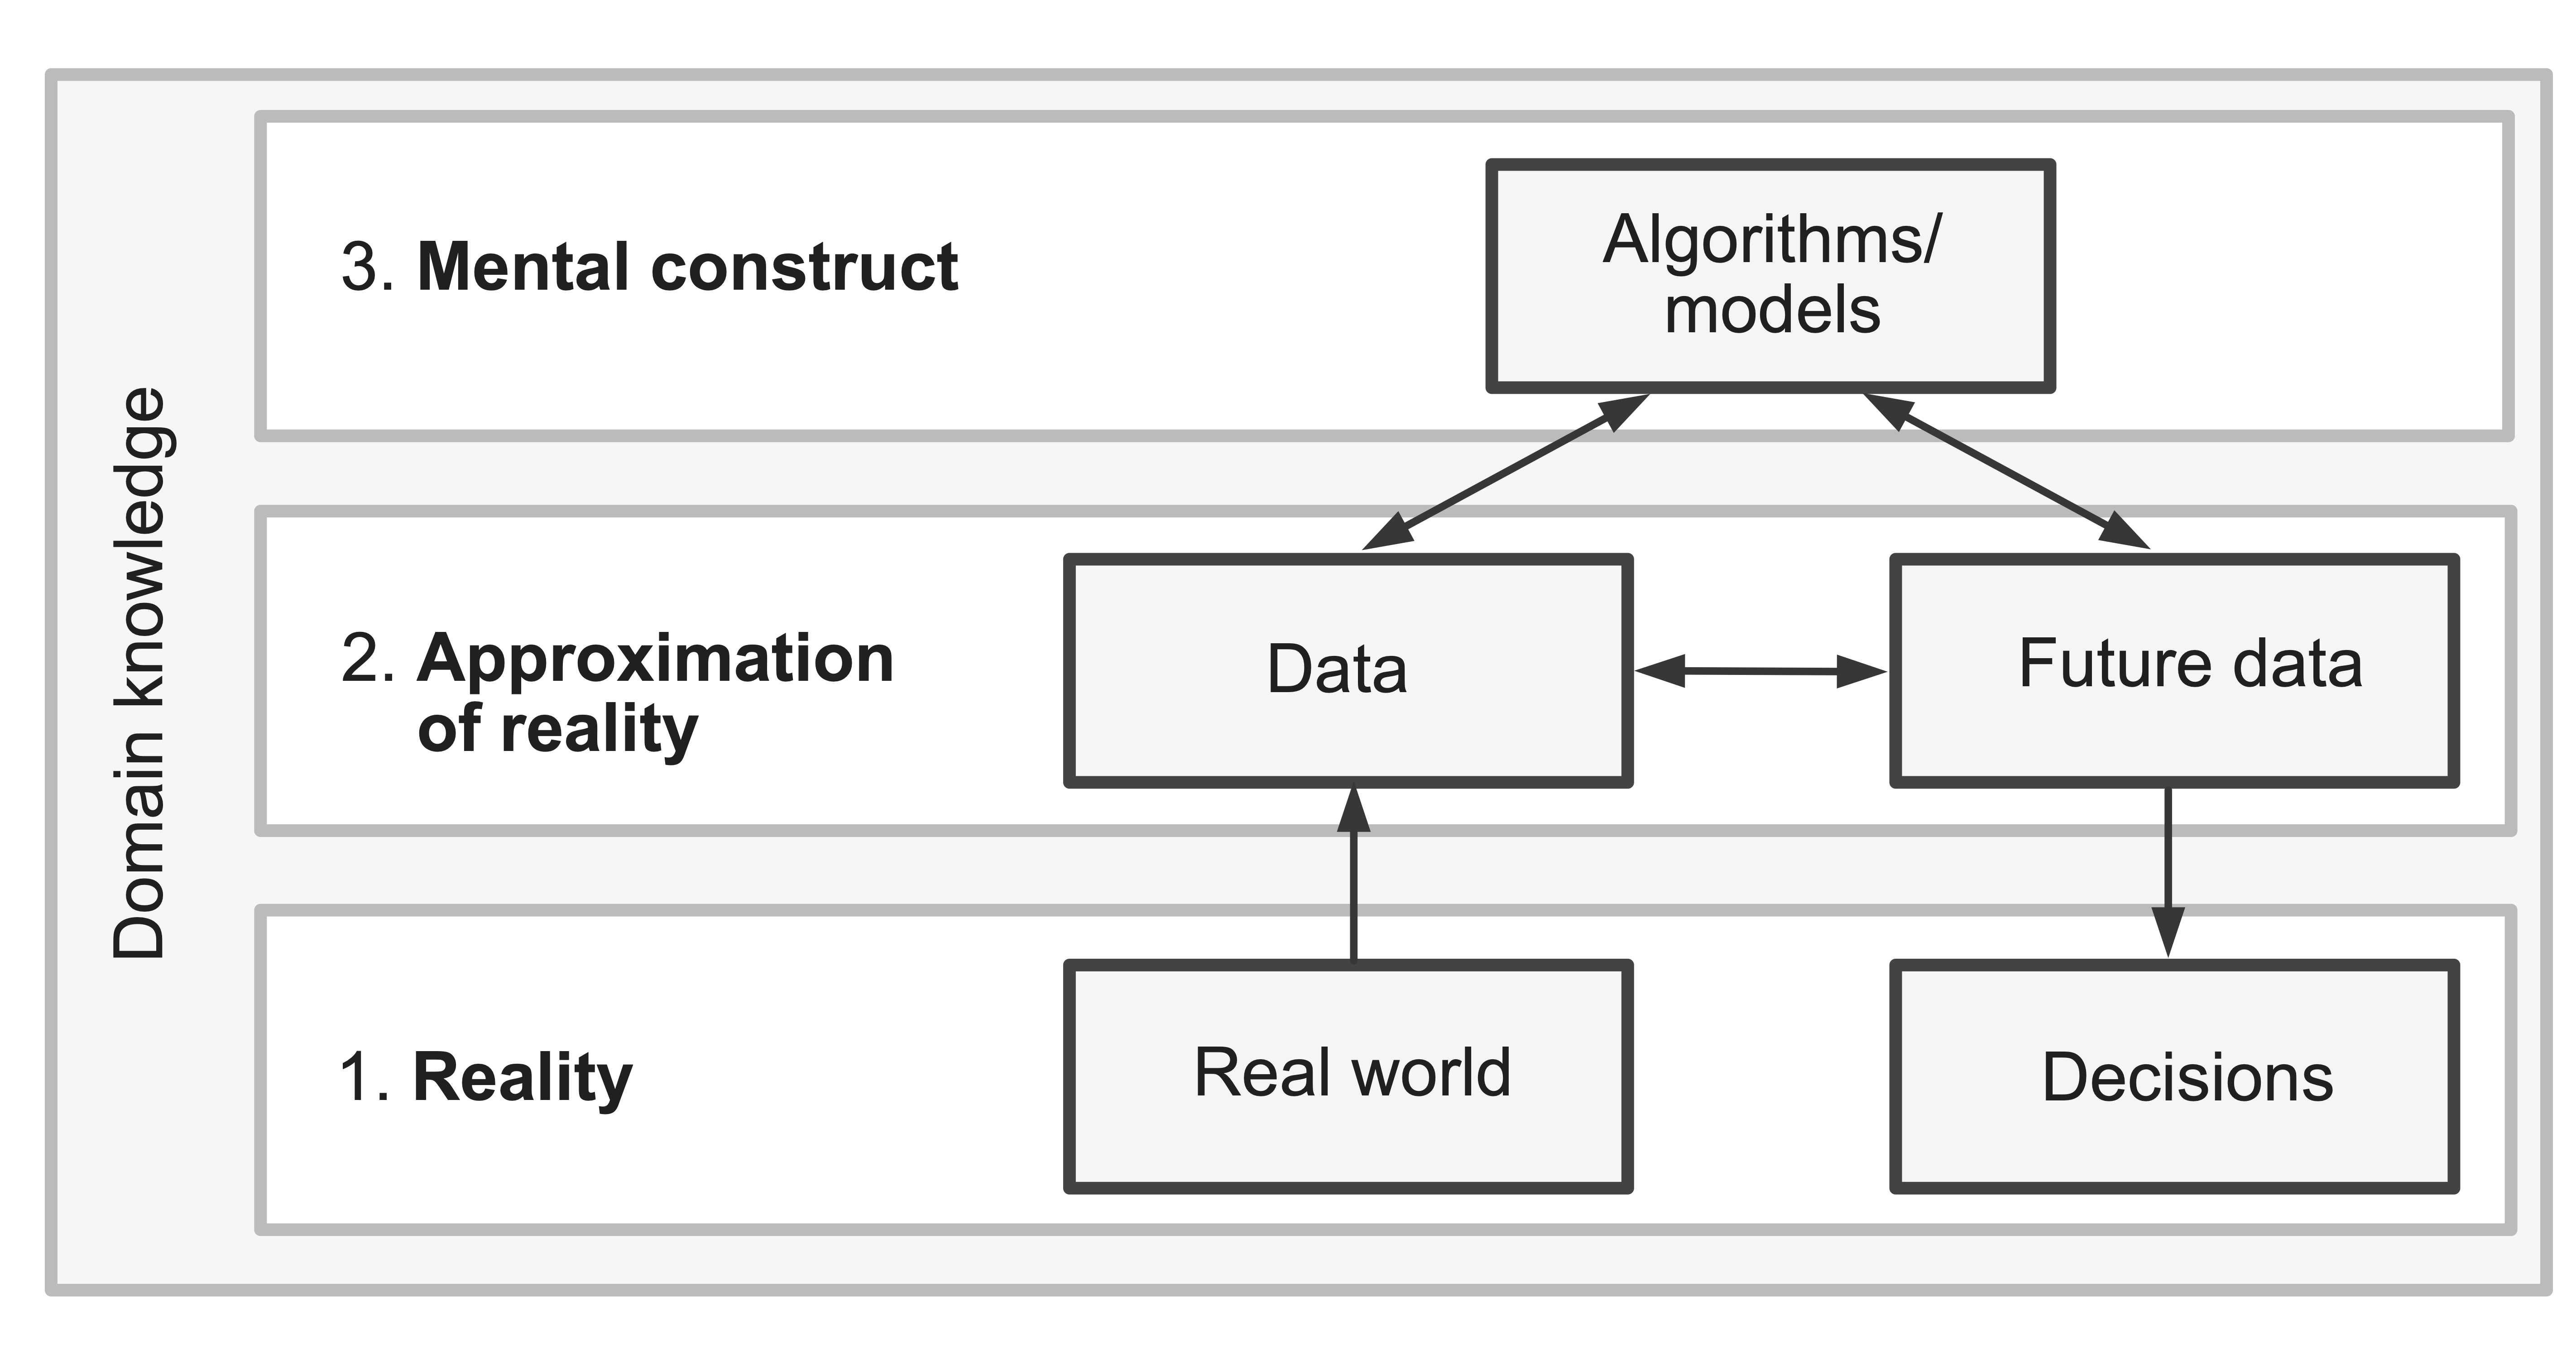
\includegraphics[width=0.8\textwidth]{gfx/m1l1_vds_fig1-1_three_realms.png}
    \caption{Ba cảnh giới: thực tế, một sự xấp xỉ của thực tế (nơi dữ liệu của chúng ta tồn tại), và cảnh giới cấu trúc tinh thần (nơi các phân tích và thuật toán của chúng ta tồn tại).}
    \label{fig:three_realms}
\end{figure}

Vấn đề là chúng ta thường không biết các kết nối giữa ba cảnh giới này mạnh đến mức nào, và việc đưa ra các quyết định thực tế dựa trên kết quả từ các thuật toán không đại diện cho thực tế (cho dù là do dữ liệu là một xấp xỉ kém của thực tế hay do sử dụng các kỹ thuật phân tích không đúng cách) có thể dẫn đến những kết quả không đáng tin cậy với hậu quả thực tiễn nghiêm trọng. Hãy xem xét ví dụ về phần mềm nhận dạng khuôn mặt. Đã có nhiều tài liệu ghi nhận rằng nhiều ứng dụng phần mềm được thiết kế để nhận dạng khuôn mặt bằng hình ảnh hoạt động tốt hơn nhiều khi nhận diện khuôn mặt của người da sáng so với người da sẫm. Một trong những nguyên nhân chính của vấn đề này là các thuật toán này được xây dựng chủ yếu bằng hình ảnh của những người có làn da sáng (tức là, dữ liệu không phản ánh sự đa dạng tồn tại trong thế giới thực) (Khalil et al. 2020). Khi dữ liệu bị thiên lệch được sử dụng để đào tạo phần mềm nhận dạng khuôn mặt, phần mềm thu được thường cũng sẽ bị thiên lệch, và khi được sử dụng trong thế giới thực, những thiên lệch này có thể dẫn đến việc làm trầm trọng thêm các bất bình đẳng xã hội hiện có.

Vì dữ liệu của bạn sẽ không thông báo cho bạn biết liệu nó có đại diện chính xác cho thực tế hay không, và các thuật toán của bạn cũng sẽ không cảnh báo bạn khi chúng được sử dụng không đúng cách, bạn cần phải thực hiện công việc của một "thám tử dữ liệu" (tư duy phản biện) để xác định xem dữ liệu của bạn có phải là một phản ánh hợp lý của thực tế hay không và liệu các thuật toán của bạn có đang được áp dụng phù hợp với dữ liệu và vấn đề chuyên ngành của bạn hay không. Trong các phần tiếp theo, chúng tôi sẽ giới thiệu một số câu hỏi tư duy phản biện giúp bạn sử dụng kiến thức chuyên ngành liên quan để đánh giá độ tin cậy của các kết quả dựa trên dữ liệu một cách định tính, thông qua việc xem xét mức độ dữ liệu phản ánh thực tế chính xác đến đâu và mức độ phân tích và thuật toán phù hợp với ngữ cảnh của dữ liệu và vấn đề. Sau đó, chúng tôi sẽ giới thiệu các nguyên tắc về khả năng dự đoán (predictability), khả năng tính toán (computability) và tính ổn định (stability) – gọi chung là PCS, mà chúng tôi sẽ sử dụng xuyên suốt cuốn sách này để đánh giá độ tin cậy của các kết quả dựa trên dữ liệu một cách định lượng, xét về khía cạnh mức độ áp dụng của kết quả đối với các kịch bản dữ liệu tương lai có liên quan và mức độ nhạy cảm của chúng đối với các nhiễu động hợp lý trong dữ liệu và quy trình phân tích của chúng ta (bao gồm cả các phán đoán của con người mà chúng ta đưa ra khi làm sạch, tiền xử lý và phân tích dữ liệu).

\subsection{Đánh giá và Xây dựng Độ tin cậy Bằng Tư duy Phản biện}

Khoa học dữ liệu không chỉ bao gồm việc làm toán và viết mã; nó còn đòi hỏi kỹ năng tư duy phản biện mạnh mẽ và nền tảng kiến thức chuyên ngành liên quan đến dự án mà bạn đang thực hiện (có thể thu được từ chuyên môn của chính bạn, internet, sách hoặc từ các cộng tác viên). Những kỹ năng này rất quan trọng để xác định các điểm yếu tiềm ẩn trong các kết nối giữa ba cảnh giới, được mô tả ở trên, và để phát hiện những thiên lệch có thể len lỏi vào quy trình thu thập và phân tích dữ liệu. Nếu không có kỹ năng tư duy phản biện vững vàng và kiến thức chuyên ngành cơ bản (thậm chí nếu chỉ là từ việc đánh giá tài liệu), bạn có nguy cơ tạo ra những kết quả gây hiểu lầm, có thể mang lại hậu quả thực tế thảm khốc.

Thật không may, số liệu thống kê và phân tích dữ liệu có tiếng xấu về độ tin cậy trong công chúng, với những câu nói như "Có ba loại nói dối: nói dối, nói dối tồi tệ và thống kê"\footnote{Việc sử dụng từ "thống kê" ở đây theo nghĩa thông tục thực chất có nghĩa là "phân tích dữ liệu".} thường làm gián đoạn các cuộc thảo luận thông thường về phân tích dữ liệu. Dù chúng tôi rất muốn nói rằng danh tiếng này là không đáng có, chúng ta không thể phủ nhận rằng rất dễ sử dụng dữ liệu để nói dối. Vấn đề là hầu hết thời gian, những lời nói dối này là vô ý, xuất phát từ việc thiếu tư duy phản biện và không xem xét kỹ lưỡng các kết quả có được từ dữ liệu (ví dụ: bằng cách sử dụng các nguyên tắc PCS mà chúng tôi sẽ giới thiệu dưới đây) trước khi trình bày chúng như là những "sự thật".

Một nhà khoa học dữ liệu thành thạo về tư duy phản biện và kiến thức chuyên ngành (và/hoặc làm việc chặt chẽ với các chuyên gia), người có hiểu biết hợp lý về các thuật toán đang được sử dụng (bao gồm các giả định và cạm bẫy liên quan), và nắm vững các nguyên tắc của PCS, sẽ ít có khả năng rơi vào cái bẫy vô tình nói dối bằng dữ liệu. Lần tới khi bạn nghe ai đó nói, “Có ba loại nói dối: nói dối, nói dối tồi tệ và thống kê,” thay vì cảm thấy bị xúc phạm, bạn có thể sửa lại: “Có ba loại nói dối: nói dối, nói dối tồi tệ và thống kê tồi.” Không phải tất cả các dự án khoa học dữ liệu đều liên quan đến phân tích dữ liệu tồi, nhưng chắc chắn là có một số!

Một số kỹ thuật tư duy phản biện mà chúng tôi khuyến nghị áp dụng trong suốt mọi dự án khoa học dữ liệu (và để đánh giá dự án của người khác) bao gồm:

\begin{itemize}
    \item \textbf{Đặt câu hỏi về vấn đề thực tiễn.} Câu hỏi đang được đặt ra có thực sự là câu hỏi mà bạn quan tâm không, và câu hỏi này ngay từ đầu có đạo đức không? Ví dụ, nếu bạn nhận được câu hỏi kinh doanh "Chúng ta có thể thay đổi tính năng nào trên trang web để khiến khách hàng ít hủy đăng ký hơn?", bạn có thể thấy rằng một câu trả lời là chuyển nút "Hủy đăng ký" đến một vị trí kín đáo hơn (tức là khó tìm hơn). Nhưng đây có thực sự là câu hỏi mà bạn muốn hỏi không? Nó có đạo đức không? Một câu hỏi tốt hơn có thể là, “Tại sao khách hàng lại có xu hướng hủy đăng ký sản phẩm của chúng ta?” Câu trả lời cho câu hỏi đó có thể giúp công ty của bạn cải thiện các dịch vụ sản phẩm (thay vì chỉ gây khó khăn cho khách hàng trong việc hủy).
    \item \textbf{Đặt câu hỏi về dữ liệu.} Dữ liệu đến từ đâu? Nguồn dữ liệu có đáng tin cậy không? Dữ liệu có liên quan đến câu hỏi đang được đặt ra, cũng như bất kỳ bối cảnh tương lai nào mà kết quả có thể được áp dụng không? Các giá trị chứa trong dữ liệu thực sự tương ứng với điều gì trong thế giới thực? Những câu hỏi này là một cách tuyệt vời để nắm bắt những điểm không nhất quán và lỗi có thể làm chệch hướng phân tích của bạn. Hãy thử tưởng tượng bản thân bạn có mặt trực tiếp trong quá trình thu thập dữ liệu. Các vấn đề tiềm ẩn nào có thể phát sinh? Bất cứ khi nào có thể, hãy làm công việc "mòn giày" (shoe-leather work) (Freedman 1991).
    \item \textbf{Đặt câu hỏi về phân tích, thuật toán và kết quả.} Những kết quả này có ý nghĩa gì trong bối cảnh thực tế? Chúng có hợp lý không? Phân tích và thuật toán có đưa ra bất kỳ giả định nào về dữ liệu hay lĩnh vực không? Những giả định này có hợp lý không? Những kết quả này có trả lời được câu hỏi chính của dự án không? Các kết quả có được truyền đạt một cách chính xác không?
\end{itemize}

Ngoài những câu hỏi này, điều quan trọng là phải theo dõi thiên kiến xác nhận (confirmation bias) và thiên kiến mong muốn (desirability bias). Thiên kiến xác nhận xảy ra khi bạn không xem xét kỹ lưỡng các kết quả một cách phản biện vì chúng khớp với những gì bạn mong đợi tìm thấy. Là con người, chúng ta có nhiều khả năng sẽ kiểm tra kỹ và soi xét kết quả khi chúng không khớp với kỳ vọng của mình (điều đó có nghĩa là chúng ta ít có khả năng phát hiện lỗi khi kết quả khớp với những gì chúng ta mong đợi). Thiên kiến mong muốn xảy ra khi bạn cố gắng tìm ra kết quả mà bạn nghĩ người khác (hoặc dư luận) mong đợi bạn tìm thấy.

Bạn có thể làm gì để giảm thiểu rủi ro của thiên kiến xác nhận và mong muốn? Mặc dù không thể hoàn toàn gạt bỏ kỳ vọng của bạn, bạn có thể rèn luyện một sự hoài nghi lành mạnh đối với mọi kết quả bạn nhận được, bất kể nó có khớp với những gì bạn hoặc người khác mong đợi hay muốn tìm thấy hay không.

\subsubsection{Nghiên cứu điển hình: Ước tính số động vật chết do cháy rừng ở Úc năm 2019}
Chúng ta hãy sử dụng các kỹ năng tư duy phản biện của mình để làm công việc thám tử, sử dụng một ví dụ từ thảm họa cháy rừng tàn phá hơn 42 triệu mẫu Anh ở bờ biển phía đông nước Úc trong nhiều tháng vào cuối năm 2019 và sang năm 2020 (để dễ hình dung, diện tích này lớn hơn toàn bộ tiểu bang Florida). Một số nhà khoa học (nổi bật nhất là Giáo sư Chris Dickman tại Đại học Sydney, người có hơn 30 năm kinh nghiệm nghiên cứu về sinh thái học, bảo tồn và quản lý động vật có vú ở Úc) ước tính rằng "hơn 1 tỷ động vật đã chết trong các vụ hỏa hoạn." Con số 1 tỷ đó là vô cùng kinh ngạc. Mặc dù hầu hết mọi người sẽ chấp nhận các báo cáo của các nghiên cứu khoa học mà không thắc mắc, chúng ta không phải là hầu hết mọi người. Hãy dành thời gian suy nghĩ nghiêm túc về nguồn gốc của con số gây kinh ngạc này, 1 tỷ, có thể đến từ đâu (không phải để hạ thấp những hậu quả kinh hoàng không thể phủ nhận của các vụ hỏa hoạn này, mà đúng hơn là để hiểu chúng rõ hơn).

\paragraph{Đặt câu hỏi về dữ liệu}

Bạn nghĩ dữ liệu làm cơ sở cho tuyên bố rằng "1 tỷ động vật đã chết trong các vụ hỏa hoạn" được thu thập như thế nào? Có phải có một nhóm các nhà khoa học đang đếm thủ công từng con vật đã chết không? Thuật ngữ "động vật" có bao gồm côn trùng, chẳng hạn như kiến và ruồi không? May mắn thay, với một chút nghiên cứu, chúng tôi đã có thể tìm thấy câu trả lời cho những câu hỏi này khá nhanh chóng. Chúng tôi khuyến khích bạn thử trả lời bất kỳ câu hỏi nào của riêng bạn. Một cuộc tìm kiếm nhanh trên internet dẫn chúng tôi đến một bài báo (Đại học Sydney 2020), trong đó tuyên bố rằng Giáo sư Dickman đã dựa trên các ước tính của mình từ một nghiên cứu chi tiết của Johnson và cộng sự (2007) (13 năm trước khi vụ hỏa hoạn xảy ra) mà Giáo sư Dickman là đồng tác giả:

"Các số liệu được Giáo sư Dickman trích dẫn dựa trên báo cáo năm 2007 của Quỹ Quốc tế Bảo vệ Thiên nhiên (WWF) về tác động của việc phát quang đất đối với động vật hoang dã ở New South Wales... [trong đó có] các ước tính về mật độ quần thể động vật có vú, chim và bò sát ở NSW" (Đại học Sydney 2020).

Bản sao PDF của cả hai bài báo này (Johnson et al. 2007) và (Đại học Sydney 2020) được cung cấp trong thư mục bushfires/ của kho lưu trữ GitHub bổ sung cho bạn đọc quan tâm.

Những gì chúng tôi tìm thấy trong quá trình tìm kiếm tài liệu của mình là những ước tính này dựa trên dữ liệu được thu thập vào năm 2007, và khi đọc thêm, chúng tôi phát hiện ra rằng nghiên cứu này chỉ bao phủ một khu vực nhỏ của bang New South Wales. Báo cáo từ Đại học Sydney (2020) cũng tuyên bố rằng "con số này bao gồm động vật có vú (không bao gồm dơi), chim và bò sát và không bao gồm ếch, côn trùng hoặc các động vật không xương sống khác."

Từ thông tin này, chúng ta có thể kết luận rằng những kết quả này không dựa trên một cơ sở dữ liệu thần bí nào đó chứa thông tin về tất cả các động vật đã chết trong hỏa hoạn, rất có thể vì không có dữ liệu nào như vậy tồn tại (và việc cố gắng tưởng tượng việc thu thập một tập dữ liệu như vậy sẽ nhanh chóng dẫn chúng ta đến kết luận rằng đây sẽ là một nhiệm vụ bất khả thi). Mặc dù dữ liệu làm nền tảng cho các kết quả đến từ một nguồn có thể xác minh và hợp pháp (nghiên cứu năm 2007 do Tổ chức Động vật Hoang dã Thế giới, một tổ chức uy tín thực hiện), điều này không tự động có nghĩa là nó liên quan đến câu hỏi đang được đặt ra. Rất nhiều thứ có thể thay đổi trong 13 năm, và thật là một tuyên bố lớn khi nói rằng các ước tính được thu thập từ một môi trường sống nhỏ, cục bộ có thể được khái quát hóa cho toàn bộ khu vực bị ảnh hưởng bởi hỏa hoạn.

Do đó, dữ liệu làm nền tảng cho nghiên cứu này là có liên quan, nhưng không nghi ngờ gì về việc nó bị hạn chế về phạm vi. Cuối cùng, Giáo sư Dickman đã làm hết sức mình với một tập dữ liệu hiện có mà ông đã quen thuộc, vì không có dữ liệu liên quan nào khác có sẵn. Thông thường, dữ liệu tốt nhất chỉ là dữ liệu bạn đang có.

\paragraph{Đặt câu hỏi về phân tích}

Với việc dữ liệu chỉ dựa trên một khu vực nhỏ, cục bộ, Giáo sư Dickman và các cộng sự của ông đã sử dụng dữ liệu như thế nào để ước tính số lượng động vật đã chết trên toàn bộ khu vực bị ảnh hưởng? Từ báo cáo của Đại học Sydney (2020), chúng ta biết được rằng

"Ước tính về mật độ quần thể động vật có vú, chim và bò sát ở NSW [thu được bằng cách nhân] các ước tính mật độ với diện tích thảm thực vật được phép phát quang" (Đại học Sydney 2020).

Chúng tôi giải thích điều này có nghĩa là họ đã lấy các ước tính năm 2007 về mật độ động vật và phóng to những con số này dựa trên kích thước của khu vực bị ảnh hưởng. Cách tiếp cận này rõ ràng không tính đến sự khác biệt về mật độ động vật trên toàn bộ khu vực bị ảnh hưởng, cũng như không tính đến cách các mật độ này có thể đã thay đổi theo thời gian. Tuy nhiên, vì không có thêm dữ liệu nào, họ có thể làm gì khác?

Mặc dù chúng ta có thể chỉ trích các kết luận dựa trên dữ liệu của người khác bao nhiêu tùy thích, nhưng trong nhiều trường hợp, đó là những con số tốt nhất (và thường là duy nhất) hiện có. Khi chỉ trích nghiên cứu của người khác, hãy luôn ghi nhớ rằng đằng sau mọi kết luận dựa trên dữ liệu là một con người có ý định tốt với những cảm xúc (điều mà mọi người thường cố tình quên). Trong trường hợp nghiên cứu của Giáo sư Dickman, mặc dù có lẽ chúng ta không nên lấy các tuyên bố như một sự thật cơ bản (chính các tác giả đã rất rõ ràng trong báo cáo của họ rằng đây là những ước tính thô và không nên hiểu theo nghĩa đen), chúng thực sự vẽ nên một bức tranh tác động sâu sắc về hậu quả tàn khốc của các vụ hỏa hoạn đối với các quần thể động vật địa phương dựa trên thông tin có sẵn. Hơn nữa, đây là nghiên cứu tầm cỡ đầu tiên thậm chí đã cố gắng định lượng tác động của các vụ hỏa hoạn đối với quần thể động vật.\footnote{Vào cuối năm 2020, một nghiên cứu mới của WWF (do Giáo sư Chris Dickman giám sát và Tiến sĩ Lily Van Eeden dẫn đầu) đã cập nhật con số này để báo cáo rằng số lượng động vật chết trong các vụ hỏa hoạn có khả năng gần 3 tỷ, một con số thậm chí còn tàn khốc hơn so với báo cáo trước đó (Vernick 2020). Nghiên cứu này chia nhỏ con số đó thành "143 triệu động vật có vú, 2,46 tỷ loài bò sát, 180 triệu loài chim và 51 triệu con ếch." Báo cáo cập nhật này chứng minh rằng các số liệu được báo cáo ban đầu không nên được hiểu theo nghĩa đen, mà thay vào đó, chúng đóng vai trò vẽ ra bức tranh tổng quát về mức độ nghiêm trọng của sự tàn phá đối với động vật hoang dã ở miền đông nước Úc.}

Bằng cách suy nghĩ phản biện về các con số được báo cáo liên quan đến tác động của các vụ hỏa hoạn này, chúng ta có thể hiểu rõ hơn nhiều về nguồn gốc của chúng và cách chúng ta nên diễn giải chúng. Trong các nghiên cứu của riêng bạn, lời khuyên của chúng tôi là hãy luôn minh bạch về các giả định làm nền tảng cho dữ liệu và kết quả của bạn và ghi chép lại chúng (công khai, nếu có thể). Mọi kết quả dựa trên dữ liệu đều có những cảnh báo (caveats), và công việc của bạn là đảm bảo rằng kết quả của mình đang được diễn giải chính xác nhất có thể.

\subsection{Đánh giá và Xây dựng Độ tin cậy Bằng Khung PCS}

Mặc dù những câu hỏi tư duy phản biện này giúp cung cấp một thước đo định tính chung về độ tin cậy của các kết quả dựa trên dữ liệu, việc cung cấp các thước đo định lượng thường cũng rất quan trọng. Đây là lúc các nguyên tắc về khả năng dự đoán (predictability), khả năng tính toán (computability) và tính ổn định (stability) – gọi chung là PCS, phát huy tác dụng. Những nguyên tắc này lần đầu tiên được giới thiệu trong Yu và Kumbier (2020), nhưng đã được mở rộng rất nhiều trong cuốn sách này.

Khung PCS cung cấp hướng dẫn và kỹ thuật để chứng minh theo kinh nghiệm rằng kết quả của bạn vượt qua một số bài kiểm tra thực tế về dự đoán và đánh giá độ ổn định nhằm giải quyết nhiều nguồn không chắc chắn liên quan đến kết quả của bạn. Ba nguyên tắc PCS là:

\begin{itemize}
    \item \textbf{Khả năng dự đoán (Predictability).} Các kết luận của bạn được coi là có thể dự đoán được nếu bạn có thể chỉ ra rằng chúng xuất hiện lại trong dữ liệu tương lai có liên quan và/hoặc phù hợp với kiến thức chuyên ngành hiện có. Các đánh giá khả năng dự đoán có thể được coi như một bài kiểm tra thực tế (reality check). Chúng tôi sẽ mở rộng nguyên tắc dự đoán trong phần tiếp theo.
    \item \textbf{Khả năng tính toán (Computability).} Khả năng tính toán là nền tảng cốt lõi cho mọi phân tích dữ liệu, đánh giá PCS và các nghiên cứu mô phỏng. Thông thường, bạn không cần phải chứng minh rằng kết quả của mình có thể tính toán được; đúng hơn là bạn sẽ sử dụng máy tính để tiến hành và đánh giá các phân tích của mình, cũng như để tạo ra các mô phỏng lấy cảm hứng từ dữ liệu.
    \item \textbf{Tính ổn định (Stability).} Kết quả của bạn được coi là ổn định nếu bạn có thể chỉ ra rằng chúng vẫn khá nhất quán khi có những sửa đổi (nhiễu động - perturbations) thực tế được thực hiện đối với dữ liệu cơ sở, các quyết định đánh giá và các lựa chọn thuật toán. Đánh giá tính ổn định có thể được coi là một tập hợp các bài kiểm tra áp lực (stress-test) đối với tính không chắc chắn liên quan đến kết quả dựa trên dữ liệu của bạn.\footnote{Lưu ý rằng khả năng dự đoán có thể được coi là một trường hợp đặc biệt của tính ổn định khi nhiễu động của dữ liệu hiện tại chính là dữ liệu tương lai.}
\end{itemize}

\begin{tcolorbox}[title={Hộp 1.2: Khung PCS}]
Khung PCS (khả năng dự đoán, khả năng tính toán và tính ổn định) cung cấp các hướng dẫn để đánh giá thực nghiệm độ tin cậy của các bằng chứng thu được từ dữ liệu ở mọi bước trong vòng đời khoa học dữ liệu (DSLC). Áp dụng các nguyên tắc PCS liên quan đến việc sử dụng các khám phá tính toán để đảm bảo kết quả của bạn có thể dự đoán được và ổn định.
\end{tcolorbox}

Các đánh giá khả năng dự đoán và độ ổn định là một phương tiện mạnh mẽ để cung cấp bằng chứng cho độ tin cậy của kết quả dựa trên dữ liệu của bạn. Tuy nhiên, chúng không cho phép bạn chứng minh rằng các kết quả dựa trên dữ liệu của bạn là chắc chắn hoàn toàn. Việc chứng minh tuyệt đối sẽ yêu cầu đánh giá khả năng dự đoán và độ ổn định một cách cạn kiệt, xem xét tất cả các kịch bản phân tích và dữ liệu thay thế có thể có — một nhiệm vụ bất khả thi. Những ý tưởng này chứa đựng tiếng vang của "Sự chứng ngụy Popper" (Popperian falsification), như được định nghĩa bởi nhà triết học Karl Popper vào những năm 1930 (Popper 2002). Chứng ngụy Popper\footnote{Trong triết học của Popper, để một phát hiện được coi là "khoa học", nó phải có "khả năng bị chứng ngụy" (falsifiable); tức là phải có thể bác bỏ nó nếu thực sự nó sai.} nói rằng một phát hiện khoa học không bao giờ thực sự được chứng minh, mà thay vào đó, mỗi kết quả thực nghiệm tích cực đều đưa ra thêm bằng chứng cho phát hiện khoa học đó.

Mặc dù bản thân khung PCS là mới, nhiều ý tưởng làm nền tảng cho nó không mới. Khung PCS nhằm mục đích thống nhất, hợp lý hóa và mở rộng các thực tiễn và ý tưởng tốt nhất từ Học máy (ML), thống kê và khoa học.

\subsubsection{Khả năng dự đoán (Predictability)}
Các nhà khoa học đã tiến hành kiểm tra thực tế khả năng dự đoán trong nhiều thế kỷ. Ví dụ, vào đầu những năm 1800, Carl Friedrich Gauss đã phát triển một mô hình dự đoán vị trí của tiểu hành tinh Ceres trên bầu trời và ông đã kiểm tra mô hình của mình (tức là ông cho thấy nó tạo ra kết quả có thể dự đoán được) bằng cách chứng minh rằng nó dự đoán chính xác vị trí tương lai thực tế của Ceres. Trong môi trường hiện đại hơn, cộng đồng Học máy (ML) từ lâu đã chứng minh khả năng dự đoán bằng cách đánh giá hiệu suất thuật toán của họ trên các tập kiểm chứng và tập kiểm tra (test/validation sets) được giữ lại. Nguyên tắc dự đoán của khung PCS mở rộng vai trò của kiến thức chuyên ngành và việc sử dụng tập kiểm chứng một cách rộng rãi, vượt ra ngoài các bài toán dự báo đơn thuần.

\begin{tcolorbox}[title={Hộp 1.3: Khả năng dự đoán}]
Kết quả dựa trên dữ liệu có thể dự đoán được nếu chúng có thể được chứng minh là xuất hiện lại (tức là có thể được khái quát hóa) trong các kịch bản mới, có liên quan. Bằng chứng mạnh mẽ về khả năng dự đoán có thể thu được bằng cách chứng minh rằng các kết quả vẫn đúng trong bối cảnh dữ liệu thực tế trong tương lai hoặc bên ngoài mà bạn sẽ áp dụng kết quả của mình. Khi không có sẵn dữ liệu tương lai/bên ngoài, một tập kiểm chứng (validation set) thay thế có thể được sử dụng để đánh giá kết quả. Bằng chứng bổ sung về khả năng dự đoán có thể thu được bằng cách chứng minh rằng các phân tích và thuật toán của bạn có khả năng khám phá ra những kết quả và mối quan hệ đã được biết đến rõ ràng trong lĩnh vực chuyên môn.
\end{tcolorbox}

Tuy nhiên, kỹ thuật đánh giá khả năng dự đoán mạnh mẽ nhất liên quan đến việc chứng minh rằng kết quả của bạn xuất hiện lại trong bối cảnh dữ liệu tương lai hoặc bên ngoài thực tế mà bạn sẽ áp dụng chúng. Ví dụ: nếu bạn đã phát triển một thuật toán dự đoán giá cổ phiếu (dựa trên dữ liệu thị trường chứng khoán trong quá khứ) và bạn muốn sử dụng thuật toán của mình để dự đoán giá cổ phiếu tương lai, bạn nên chứng minh rằng thuật toán của bạn tạo ra các dự đoán chính xác cho dữ liệu thị trường chứng khoán trong một khoảng thời gian diễn ra sau thời điểm của dữ liệu ban đầu được sử dụng để "huấn luyện" thuật toán. Lấy một ví dụ khác, hãy tưởng tượng rằng bạn đang tiến hành một phân tích để cố gắng hiểu các yếu tố rủi ro nhiễm trùng tại bệnh viện bằng cách sử dụng dữ liệu thu thập từ các bệnh nhân tại bệnh viện nơi bạn làm việc. Nếu bạn định áp dụng những phát hiện của mình cho bệnh nhân từ các bệnh viện khác, thì bạn nên chứng minh rằng các yếu tố rủi ro mà bạn đã xác định cũng có liên quan đến bệnh nhân ở các bệnh viện khác.

Tuy nhiên, có nhiều tình huống bạn không có quyền truy cập vào bất kỳ dữ liệu bên ngoài hoặc tương lai nào phản ánh bối cảnh mà bạn định áp dụng kết quả hoặc thuật toán của mình. Trong những tình huống này, bạn có thể mô phỏng dữ liệu tương lai hoặc bên ngoài bằng cách giữ lại một phần dữ liệu ban đầu của mình trước khi tiến hành phân tích với mục đích duy nhất là đánh giá khả năng dự đoán cho kết quả của bạn. Dữ liệu bị giữ lại này có thể đóng vai trò như một dữ liệu thay thế (surrogate) cho dữ liệu tương lai. Bằng chứng bổ sung về khả năng dự đoán cho kết quả của bạn có thể thu được từ việc chứng minh rằng các phân tích và thuật toán của bạn có khả năng nắm bắt các kết quả và mối quan hệ được biết đến rõ ràng trong lĩnh vực (xem mục bằng chứng chuyên môn).

\paragraph{Tập dữ liệu Huấn luyện, Kiểm chứng và Kiểm tra}

Trong trường hợp không có sẵn dữ liệu tương lai/bên ngoài, kỹ thuật được khuyên dùng để tạo các tập dữ liệu thay thế cho bên ngoài/tương lai là chia dữ liệu của bạn thành một tập huấn luyện (training set) và một tập kiểm chứng (validation set) (và có thể cả tập kiểm tra - test set), như phổ biến trong cộng đồng ML.

Tập huấn luyện (dữ liệu huấn luyện/tập dữ liệu huấn luyện) là phần lớn nhất của dữ liệu (nên chứa ít nhất 50\% dữ liệu ban đầu; chúng tôi thường sử dụng 60\%), và đây là dữ liệu mà bạn sẽ sử dụng để tiến hành khám phá, phân tích và huấn luyện các thuật toán của mình.

Mục đích của tập kiểm chứng (dữ liệu kiểm chứng/tập dữ liệu kiểm chứng) (chúng tôi thường sử dụng 20\% đến 40\% dữ liệu ban đầu, tùy thuộc vào việc chúng ta có tạo tập kiểm tra hay không) là để cung cấp một đánh giá độc lập về kết quả hoặc thuật toán của bạn: nghĩa là, để chứng minh rằng kết quả của bạn xuất hiện lại (hoặc thuật toán của bạn hoạt động tốt) trong dữ liệu giống với dữ liệu tương lai mà kết quả của bạn sẽ được áp dụng. Do đó, tập dữ liệu kiểm chứng nên được tạo theo cách phản ánh tốt nhất dữ liệu thực tế bên ngoài hoặc tương lai mà kết quả của bạn có thể được sử dụng để đưa ra quyết định trong thế giới thực. Thông thường, kết quả của tập dữ liệu kiểm chứng sẽ được sử dụng để quyết định giữa một số phân tích hoặc thuật toán thay thế, hoặc để lọc ra các thuật toán hoạt động kém (điều này đặc biệt phổ biến trong các bài toán dự đoán). Trong trường hợp đó, vì tập dữ liệu kiểm chứng của bạn đã được sử dụng để tạo ra kết quả cuối cùng của bạn, việc sử dụng một tập dữ liệu bị giữ lại khác để cung cấp một đánh giá độc lập về kết quả cuối cùng của bạn trở nên quan trọng.

Đây là lúc tập kiểm tra (dữ liệu kiểm tra/tập dữ liệu kiểm tra) phát huy tác dụng. Tập kiểm tra sẽ bao gồm phần dữ liệu còn lại chưa được sử dụng trong các tập huấn luyện hoặc kiểm chứng, thường là 20\% dữ liệu ban đầu. Tập dữ liệu kiểm tra có thể được sử dụng để cung cấp đánh giá độc lập cuối cùng về một thuật toán đã được chọn dựa trên hiệu suất ở tập kiểm chứng. Tương tự như tập dữ liệu kiểm chứng, tập dữ liệu kiểm tra phải giống với dữ liệu tương lai mà kết quả của bạn sẽ được áp dụng càng sát càng tốt.

Nếu bạn sẽ sử dụng các tập kiểm chứng (và kiểm tra) để đánh giá kết quả dựa trên dữ liệu của mình, điều quan trọng là bạn phải dành riêng các phần dữ liệu này trước khi bắt đầu tiến hành phân tích.

\begin{tcolorbox}[title={Hộp 1.4: Vai trò của Tập dữ liệu Huấn luyện, Kiểm chứng và Kiểm tra}]
Khi bạn không có quyền truy cập vào dữ liệu tương lai/bên ngoài để sử dụng cho việc đánh giá khả năng dự đoán, bạn có thể chia dữ liệu hiện tại của mình thành hai hoặc ba phần.

Phần đầu tiên là dữ liệu huấn luyện (thường chiếm khoảng 60\% dữ liệu ban đầu), được sử dụng để khám phá các mô hình, mối quan hệ tiềm ẩn trong dữ liệu và đào tạo thuật toán.

Phần thứ hai là dữ liệu kiểm chứng (thường chiếm khoảng 20\% đến 40\% dữ liệu ban đầu), được sử dụng để đánh giá kết quả và thuật toán bằng cách đóng vai trò như một vật thay thế cho dữ liệu trong tương lai.

Nếu bạn sẽ sử dụng tập dữ liệu kiểm chứng để so sánh nhiều phân tích hoặc thuật toán thay thế nhằm chọn ra kết quả cuối cùng, thì một tập dữ liệu kiểm tra bổ sung (thường chiếm khoảng 20\% dữ liệu ban đầu) nên được đặt sang một bên để cung cấp một lớp xem xét độc lập bổ sung đối với các kết quả cuối cùng. Tập kiểm tra đóng vai trò là vật thay thế cuối cùng cho dữ liệu tương lai.

Dữ liệu nên được phân chia theo cách thức (ví dụ: sử dụng phân chia ngẫu nhiên, theo nhóm hoặc theo thời gian) sao cho mối quan hệ giữa dữ liệu huấn luyện với dữ liệu kiểm chứng/kiểm tra phản ánh đúng mối quan hệ giữa dữ liệu hiện tại và dữ liệu tương lai mà kết quả và thuật toán sẽ được áp dụng.
\end{tcolorbox}

Nếu bạn đang chia dữ liệu của mình thành các tập dữ liệu huấn luyện, kiểm chứng và kiểm tra, bạn nên thực hiện theo cách sao cho các tập kiểm chứng và kiểm tra phản ánh dữ liệu tương lai/bên ngoài mà bạn định áp dụng kết quả của mình. Các cơ chế chia phổ biến bao gồm:

\begin{itemize}
    \item \textbf{Chia theo thời gian (Time-based split):} Nếu dữ liệu của bạn được thu thập theo thời gian và bạn sẽ áp dụng một thuật toán mà bạn đã huấn luyện cho dữ liệu tương lai, thì cách chia huấn luyện/kiểm chứng/kiểm tra sử dụng 60\% dữ liệu cũ nhất của bạn làm tập dữ liệu huấn luyện, và chia đều 40\% dữ liệu mới hơn giữa tập kiểm chứng và kiểm tra là sự thể hiện tốt mối quan hệ giữa dữ liệu hiện tại và tương lai. Ví dụ, nếu bạn có 10 năm dữ liệu thị trường chứng khoán, bạn có thể sử dụng giá cổ phiếu từ 6 năm đầu làm dữ liệu huấn luyện, sau đó dùng giá cổ phiếu từ 4 năm cuối cho tập kiểm chứng và kiểm tra để đánh giá. Tuy nhiên, trên thực tế, sau khi bạn đã tiến hành đánh giá, bạn có thể muốn huấn luyện lại thuật toán của mình bằng tất cả dữ liệu có sẵn để đảm bảo rằng thuật toán của bạn nắm bắt được những xu hướng cập nhật nhất có thể.
    \item \textbf{Chia theo nhóm (Group-based split):} Nếu dữ liệu của bạn có sự phân nhóm tự nhiên (ví dụ: dữ liệu bao gồm thông tin từ bệnh nhân ở một vài bệnh viện khác nhau) và bạn sẽ áp dụng một thuật toán bạn huấn luyện cho một nhóm điểm dữ liệu mới (ví dụ: bệnh nhân ở một bệnh viện khác), thì bạn có thể chọn ngẫu nhiên một tập con 60\% các nhóm (ví dụ: bệnh viện, thay vì bệnh nhân) để tạo tập dữ liệu huấn luyện, sau đó chia đều các nhóm còn lại giữa tập kiểm chứng và kiểm tra. Điều này đảm bảo rằng mọi điểm dữ liệu từ cùng một nhóm sẽ được chứa hoàn toàn trong một tập huấn luyện, hoặc kiểm chứng, hoặc kiểm tra, chứ không bị phân mảnh, và nó phản ánh tốt nhất quá trình áp dụng thuật toán cho các điểm dữ liệu ở nhóm mới.
    \item \textbf{Chia ngẫu nhiên (Random split):} Sử dụng cách chia ngẫu nhiên thuần túy để tạo các tập dữ liệu kiểm chứng và kiểm tra (tức là chọn ngẫu nhiên hai tập, mỗi tập 20\% số điểm dữ liệu để tạo tập kiểm chứng và kiểm tra) là hợp lý khi các điểm dữ liệu hiện tại đều có thể hoán đổi cho nhau ít nhiều (ví dụ: khi mọi người được chọn ngẫu nhiên tham gia một cuộc khảo sát) và các điểm dữ liệu mới mà bạn sẽ áp dụng kết quả cũng tương tự (ví dụ: bạn khái quát hóa kết quả cho những người không được khảo sát, nhưng có thể đã được).
\end{itemize}

Bất kể loại phân chia nào bạn chọn, bạn luôn phải chứng minh tại sao lựa chọn của bạn cung cấp một sự thay thế tốt cho dữ liệu tương lai (hoặc bên ngoài) có liên quan bằng cách sử dụng kiến thức chuyên ngành, sự hiểu biết của bạn về quá trình thu thập dữ liệu, và cách kết quả hoặc thuật toán của bạn sẽ được sử dụng (ví dụ: chúng sẽ được áp dụng cho loại dữ liệu tương lai nào).

Lưu ý rằng không cần cảm thấy bị ràng buộc vào tỷ lệ 60/40 (hoặc 60/20/20): bạn có thể chọn tỷ lệ nào bạn cảm thấy thoải mái, mặc dù chúng tôi khuyên bạn nên tạo một tập dữ liệu huấn luyện chứa ít nhất 50\% dữ liệu của bạn.

Xin nhắc lại, chúng tôi thực sự khuyên bạn nên chia dữ liệu của mình thành các tập dữ liệu huấn luyện, kiểm chứng và kiểm tra trước khi bạn bắt đầu khám phá và phân tích dữ liệu (mặc dù bạn vẫn có thể thực hiện một số khám phá nhẹ trước khi chia để nắm bắt cấu trúc dữ liệu). Việc phân chia dữ liệu ở những giai đoạn rất sớm của dự án sẽ giúp ngăn chặn rò rỉ dữ liệu (data leakage), khi thông tin từ tập huấn luyện "rò rỉ" sang tập kiểm chứng và kiểm tra (và ngược lại), làm suy giảm khả năng của các tập kiểm chứng và kiểm tra đóng vai trò như một sự thay thế hợp lý cho dữ liệu tương lai hoặc bên ngoài hoàn toàn độc lập (Kaufman et al. 2012).

Do đó, điều quan trọng là phải lập kế hoạch về cách bạn sẽ đánh giá khả năng dự đoán của kết quả ở giai đoạn rất sớm trong dự án của bạn (lý tưởng nhất là ngay khi bạn thu thập xong dữ liệu).

\paragraph{Vai trò của Bằng chứng Chuyên môn trong việc Chứng minh Khả năng Dự đoán}

Mặc dù chúng ta sẽ chủ yếu sử dụng dữ liệu bên ngoài/kiểm chứng để đánh giá khả năng dự đoán của kết quả, một kỹ thuật khác mà chúng ta đôi khi sử dụng để chứng minh khả năng dự đoán của kết quả là cho thấy rằng phân tích hoặc thuật toán của chúng ta phát hiện ra các mô hình hoặc mối quan hệ được thiết lập tốt trong lĩnh vực (ví dụ: từ các bài báo nghiên cứu được bình duyệt có uy tín).

Ví dụ: nếu chúng ta phát triển một thuật toán xác định mối liên hệ giữa kiểu gen (gen) và kiểu hình (đặc điểm thể chất), và chúng ta có thể chỉ ra rằng thuật toán của mình có khả năng phát hiện ra các mối quan hệ kiểu gen - kiểu hình đã biết (ví dụ: kết quả của chúng ta cho thấy một gen được ghi chép nhiều trong tài liệu có liên quan đến việc có mái tóc đỏ thực sự có liên quan đến kiểu hình tóc đỏ), thì chúng ta có thể sử dụng điều này làm bằng chứng cho khả năng dự đoán của thuật toán, từ đó cung cấp bằng chứng về độ tin cậy của bất kỳ mối quan hệ mới nào mà chúng ta xác định được. Đây là một ví dụ về việc sử dụng nguyên tắc khả năng dự đoán như một bài kiểm tra thực tế.

\subsubsection{Tính ổn định (Stability)}
Trụ cột thứ hai của khung PCS là tính ổn định. Để hiểu nguyên lý ổn định, hãy xem xét phép ẩn dụ sau. Đối với mỗi bức ảnh mà bạn chụp, có nhiều bức ảnh thay thế hợp lý khác mà bạn có thể đã chụp, nhưng không chụp. Ví dụ, bức ảnh có thể được chụp sau 30 giây, hoặc bạn có thể đứng sang trái ba bước. Dữ liệu chúng ta thu thập cũng vậy. Đối với mọi tập dữ liệu mà chúng ta thu thập, có nhiều tập dữ liệu thay thế hợp lý mà chúng ta có thể đã thu thập, chẳng hạn như nếu người khác ghi lại các phép đo, nếu chúng được đo vào một ngày khác, hoặc nếu các phép đo được thực hiện cho một nhóm cá nhân hơi khác một chút.

Tuy nhiên, phép ẩn dụ của chúng ta không dừng lại ở giai đoạn thu thập dữ liệu. Sau khi chúng ta chụp ảnh, có rất nhiều bộ lọc tiền xử lý mà chúng ta có thể sử dụng để sửa đổi nó, thường với mục đích làm cho bức ảnh trông giống với thế giới thực mà chúng ta nhìn thấy bằng mắt hơn. Các lựa chọn xử lý mà chúng ta thực hiện ở đây là những đánh giá cá nhân (judgment calls). Do đó, đối với bất kỳ bức ảnh nhất định nào mà chúng ta chụp, có nhiều sản phẩm cuối cùng thay thế mà chúng ta có thể tạo ra, là kết quả của việc chụp một bức ảnh hơi khác và/hoặc sử dụng các kỹ thuật tiền xử lý hơi khác nhau.

Sự tương tự trong khoa học dữ liệu là có nhiều cách thay thế mà chúng ta có thể chọn để làm sạch hoặc tiền xử lý dữ liệu (ví dụ: có nhiều cách để điền dữ liệu khuyết thiếu) cũng như phân tích dữ liệu (ví dụ: có thể có nhiều thuật toán thực hiện cùng một tác vụ), dẫn đến một loạt các kết quả xuôi dòng (downstream results) khả dĩ mà chúng ta có thể đạt được. Sự không chắc chắn nằm bên dưới quy trình thu thập dữ liệu cùng những đánh giá chủ quan trong làm sạch và phân tích biểu hiện thành sự không chắc chắn trong kết quả của chúng ta.

Đối với hầu hết các dự án khoa học dữ liệu, không có một tập dữ liệu "đúng" duy nhất để thu thập, cũng không có một cách "đúng" duy nhất để làm sạch hoặc phân tích nó. Thay vào đó, có nhiều tập dữ liệu tương đương mà bạn có thể thu thập, nhiều cơ chế làm sạch dữ liệu thay thế mà bạn có thể triển khai và nhiều phân tích mà bạn có thể tiến hành, mỗi phân tích đều có thể biện minh bằng kiến thức chuyên môn tương đương. Câu hỏi đặt ra là: Xuyên suốt phổ các tập dữ liệu, thủ tục làm sạch và phân tích hợp lý mà chúng ta có thể tiến hành, các kết quả thay thế mà chúng ta có thể đạt được có độ biến thiên ra sao? Nếu câu trả lời là "rất biến thiên," thì kết quả của chúng ta rõ ràng rất nhạy cảm với các lựa chọn nhỏ nhặt được thực hiện trong quá trình tạo ra chúng, và câu hỏi trở thành: Chúng ta có nên tin tưởng rằng tập hợp kết quả cụ thể mà chúng ta tạo ra phản ánh chính xác thực tế không? Chúng ta có thể tìm một câu trả lời gần đúng cho câu hỏi này bằng cách tiến hành phân tích tính ổn định.\footnote{Chúng tôi đã chính thức giới thiệu nguyên lý ổn định trong bối cảnh lập mô hình thống kê trong bài báo “Stability” (Yu 2013) và nguyên lý ổn định đã được mở rộng trong bài viết gốc “Veridical Data Science” (Yu và Kumbier 2020), và thậm chí còn sâu hơn trong cuốn sách này.}

Cũng giống như nguyên lý khả năng dự đoán, các ý tưởng làm nền tảng cho nguyên lý ổn định có một lịch sử lâu dài. Tính ổn định là sự mở rộng của khái niệm đánh giá độ không chắc chắn (uncertainty assessment) từ thống kê cổ điển (cũng như tính ổn định trong phân tích số và lý thuyết điều khiển). Không chắc chắn, trong bối cảnh này, đề cập đến các cách thức mà kết quả của chúng ta có thể trông khác đi dưới các kịch bản khác nhau.

Quan điểm thống kê cổ điển về tính không chắc chắn chỉ xem xét một nguồn gốc sự không chắc chắn, dựa trên việc đặt câu hỏi về việc kết quả sẽ khác đi như thế nào nếu một mẫu ngẫu nhiên thay thế được thu thập; tức là, nó chỉ xem xét biến động mẫu dưới một quy trình thu thập/lấy mẫu ngẫu nhiên giả thuyết. Tuy nhiên, nguyên lý ổn định của khoa học dữ liệu chân thực xem xét một phạm vi rộng lớn hơn nhiều các nguồn không chắc chắn, đặt câu hỏi về việc kết quả sẽ khác như thế nào nếu dữ liệu thay thế được thu thập (theo những cách vượt ra ngoài các mẫu ngẫu nhiên thay thế), cũng như nếu chúng ta đưa ra các đánh giá chủ quan về làm sạch, tiền xử lý và phân tích thay thế. Do đó, nguyên lý ổn định có thể được coi là một sự mở rộng của các khái niệm truyền thống về tính không chắc chắn thống kê, cũng như tính vững của thống kê (statistical robustness), tập trung vào việc tìm kiếm các công cụ ước lượng tham số thống kê ổn định trên nhiều cơ chế và phân phối thu thập dữ liệu thống kê.

Trong cuốn sách này, chúng tôi chủ yếu giải quyết ba nguồn không chắc chắn phát sinh từ: (1) quy trình thu thập dữ liệu bằng cách sử dụng các nhiễu động dữ liệu (data perturbations) thích hợp; (2) các đánh giá cá nhân (judgment calls) trong làm sạch và tiền xử lý dữ liệu; và (3) sự lựa chọn thuật toán được sử dụng. Nếu kết quả của bạn sụp đổ khi bạn đưa ra các phán đoán thay thế ở bất kỳ giai đoạn nào trong số này, điều đó cho thấy chúng không ổn định. Ba đánh giá về tính không chắc chắn mà chúng tôi tập trung vào không bao quát hết — sẽ luôn có những nguồn không chắc chắn bổ sung mà chúng ta chưa xem xét. Tuy nhiên, sẽ là không thể để giải quyết mọi nguồn không chắc chắn tiềm ẩn. Do đó, mục tiêu của chúng tôi là đánh giá một vài nguồn không chắc chắn khác nhau để cung cấp nhiều góc độ bằng chứng về tính ổn định của kết quả của chúng ta.

Một cách để điều tra sự không chắc chắn liên quan đến việc thu thập dữ liệu là tính toán lại kết quả bằng cách sử dụng các phiên bản bị nhiễu động nhẹ của dữ liệu, trong đó các nhiễu động được biện minh dựa trên quá trình thu thập dữ liệu ban đầu và nhằm mục đích đại diện cho các tập dữ liệu thay thế tiềm năng có thể đã được tạo ra. Tương tự, chúng ta có thể điều tra sự không chắc chắn liên quan đến các đánh giá cá nhân mà chúng ta đưa ra khi làm sạch và tiền xử lý dữ liệu bằng cách so sánh các kết quả được tính toán trên các phiên bản thay thế của dữ liệu đã được làm sạch và tiền xử lý dựa trên các đánh giá thay thế mà chúng ta có thể thực hiện (ví dụ: quy khuyết bằng trung bình thay vì trung vị). Nếu các phiên bản thay thế của kết quả khá giống nhau, điều này chỉ ra rằng độ không chắc chắn không quá khắc nghiệt và kết quả khá ổn định, điều này có thể được sử dụng như bằng chứng về độ tin cậy.

\begin{tcolorbox}[title={Hộp 1.5: Tính ổn định}]
Kết quả dựa trên dữ liệu là ổn định nếu chúng có xu hướng không thay đổi giữa các nhiễu động thay thế hợp lý xuyên suốt vòng đời khoa học dữ liệu (DSLC). Mục tiêu của một phân tích ổn định PCS là cố gắng khám phá nhiều nguồn không chắc chắn có liên quan; tức là những cách mà kết quả của chúng ta có thể có sự khác biệt một cách hợp lý. Mặc dù không thể khám phá tất cả sự không chắc chắn liên quan đến mỗi kết quả, nhưng mục tiêu của chúng ta là đánh giá tính ổn định của các kết quả của mình trên các nhiễu động hợp lý (được chứng minh bằng kiến thức chuyên môn) đối với quy trình thu thập dữ liệu, các đánh giá chủ quan trong làm sạch và tiền xử lý dữ liệu của chính chúng ta, cũng như các lựa chọn thuật toán.
\end{tcolorbox}

Lưu ý rằng kỹ thuật đánh giá khả năng dự đoán của việc đánh giá kết quả bằng cách sử dụng dữ liệu tương lai (hoặc dữ liệu tương lai giả, chẳng hạn như tập kiểm chứng) có thể được coi là một trường hợp đặc biệt của việc đánh giá tính ổn định của kết quả đối với nhiễu động của dữ liệu. Những người quen thuộc với Học máy (ML) cũng có thể nhận ra tính ổn định là một khái niệm liên quan đến các nhiệm vụ học chuyển giao (bao gồm cả thích ứng miền), trong đó một thuật toán được huấn luyện để giải quyết vấn đề trong một kịch bản được điều chỉnh lại để giải quyết vấn đề ở kịch bản khác.

\subsubsection{Khả năng tính toán (Computability)}
Mặc dù nó không được làm nổi bật nhiều trong các cuộc thảo luận của chúng ta về khung PCS, trụ cột về khả năng tính toán đóng một vai trò hỗ trợ quan trọng xuyên suốt mọi phân tích dữ liệu và đánh giá PCS. Mặc dù trọng tâm chính của cuốn sách này là phân tích dữ liệu thực tế, vai trò của khả năng tính toán lại nổi lên hàng đầu trong bối cảnh các nghiên cứu mô phỏng lấy cảm hứng từ dữ liệu, vượt ngoài phạm vi của cuốn sách này. Mặc dù chúng tôi không thảo luận sâu rộng về nguyên lý khả năng tính toán trong suốt cuốn sách, nhưng mỗi khi chúng tôi sử dụng máy tính để tiến hành phân tích hoặc đánh giá PCS, chúng tôi cố gắng đảm bảo rằng các tính toán của mình rõ ràng, hiệu quả, có thể mở rộng và có thể tái tạo, điều này phản ánh bản chất của nguyên lý tính toán.

\subsubsection{PCS như một Sự thống nhất của các Nền văn hóa}
Để kết thúc chương này, chúng tôi cung cấp một cuộc thảo luận ngắn về các nguyên tắc PCS như một sự thống nhất và mở rộng của nền văn hóa suy luận thống kê truyền thống biệt lập trước đây và nền văn hóa học máy hiện đại được phác thảo bởi Breiman (2001) (mặc dù thuật ngữ của ông khác với chúng ta). Nền văn hóa suy luận thống kê truyền thống liên hệ các phát hiện dựa trên dữ liệu với thế giới thực, đặt câu hỏi về mức độ kết quả có thể thay đổi trong ranh giới cách dữ liệu được tạo ra (tức là bằng cách nghiên cứu tính không chắc chắn của kết quả xuất phát từ quy trình lấy mẫu dữ liệu ngẫu nhiên giả định), trong khi nền văn hóa ML hiện đại đánh giá các kết quả thuật toán bằng cách chỉ ra rằng chúng cũng hoạt động tốt khi áp dụng cho dữ liệu được giữ lại (tập kiểm chứng) (tức là bằng cách chứng minh khả năng dự đoán của kết quả). Trong khoa học dữ liệu chân thực, chúng tôi mở rộng, khái quát hóa và thống nhất các ý tưởng từ cả hai nền văn hóa, đồng thời kết hợp kiến thức chuyên môn và xem xét các kịch bản thế giới thực mà kết quả của chúng tôi sẽ được áp dụng. Để có cuộc thảo luận chuyên sâu hơn về cách khoa học dữ liệu chân thực mở rộng và thống nhất hai nền văn hóa của Brieman, hãy xem bài báo của chúng tôi “The Data Science Process: One Culture” (Yu và Barter 2020).

\section*{Bài tập}

\subsection*{Bài tập Đúng hay Sai}
Đối với mỗi câu hỏi, hãy chỉ định xem câu trả lời là đúng hay sai (giải thích ngắn gọn câu trả lời của bạn).

1. Dữ liệu luôn là một sự xấp xỉ tốt của thực tế.

2. Với việc rèn luyện, bạn có thể loại bỏ hoàn toàn thiên kiến xác nhận.

3. Kết quả tính toán từ một tập dữ liệu được thu thập ngày hôm nay có thể không áp dụng được cho dữ liệu sẽ được thu thập trong tương lai, ngay cả khi cả hai tập dữ liệu được thu thập bằng cùng một cơ chế.

4. Ngay khi phân tích của bạn cung cấp câu trả lời cho câu hỏi chuyên ngành của bạn, bạn đã trả lời kết luận dứt khoát cho câu hỏi đó.

5. Có nhiều cách để chứng minh khả năng dự đoán của kết quả.

\subsection*{Bài tập Khái niệm}
6. Giải thích tại sao một phát hiện có nguồn gốc từ dữ liệu nên được coi là bằng chứng chứ không phải là bằng chứng chắc chắn (proof) của một hiện tượng thực tế.

7. Mô tả ít nhất hai nguồn không chắc chắn gắn liền với mọi kết quả dựa trên dữ liệu.

8. Mô tả hai kỹ thuật (định lượng hoặc định tính) mà bạn có thể sử dụng để củng cố bằng chứng về độ tin cậy của một phát hiện dựa trên dữ liệu.

9. Liệt kê ít nhất hai lý do tại sao các tính toán của Giáo sư Dickman có thể không phản ánh hoàn hảo số lượng động vật thực sự đã chết trong các vụ cháy rừng ở Úc.

10. Hãy tưởng tượng rằng bạn có vô số nguồn lực (nhân lực, thời gian, tiền bạc, v.v.) theo ý mình. Đối với ví dụ về thảm họa cháy rừng ở Úc, hãy mô tả dữ liệu giả định mà bạn sẽ thu thập và cách bạn sẽ thu thập nó để trả lời câu hỏi có bao nhiêu động vật đã chết trong các vụ cháy một cách chính xác nhất có thể. Hãy cụ thể. Bạn sẽ đo các giá trị nào và bạn sẽ đo chúng bằng phương pháp vật lý như thế nào? (Giả sử rằng bạn có một cỗ máy thời gian và có thể quay ngược thời gian về khoảng thời gian ngay sau khi có hỏa hoạn để thu thập dữ liệu nếu bạn muốn).

11. Bằng lời của bạn, hãy tóm tắt ngắn gọn các yếu tố về khả năng dự đoán và độ ổn định của PCS cho một thành viên gia đình hoàn toàn không có chuyên môn kỹ thuật.

12. Vai trò của tập dữ liệu kiểm chứng trong việc đánh giá khả năng dự đoán của một kết quả dựa trên dữ liệu là gì?

13. Mô tả một kỹ thuật mà bạn có thể sử dụng để đánh giá tính ổn định của kết quả dựa trên dữ liệu.

14. Kỹ thuật chia nào (dựa trên nhóm, dựa trên thời gian hoặc ngẫu nhiên) sẽ thích hợp nhất để tạo ra một phần chia tập dữ liệu huấn luyện, kiểm chứng và kiểm tra trong từng kịch bản sau:

a. Sử dụng dữ liệu thời tiết lịch sử để phát triển thuật toán dự báo thời tiết

b. Sử dụng dữ liệu từ trẻ em ở 10 trường học ở California để đánh giá mối quan hệ giữa quy mô lớp học và điểm kiểm tra ở các trường khác trong bang California

c. Sử dụng dữ liệu từ các cuộc bầu cử trước đây để phát triển thuật toán dự đoán kết quả của cuộc bầu cử sắp tới

d. Sử dụng dữ liệu từ một tập hợp con ngẫu nhiên khách truy cập một cửa hàng trực tuyến để xác định các đặc điểm nào liên quan đến việc khách hàng mua hàng.

\subsection*{Bài tập Đọc}
Các tệp PDF chứa từng bài báo được liệt kê ở đây có thể được tìm thấy trong thư mục exercises/reading trên kho lưu trữ GitHub bổ sung.

15. Đọc bài “Statistical Modeling: The Two Cultures” của Breiman (2001) và viết một bản tóm tắt ngắn về mối liên hệ của nó với khung PCS. Đừng lo lắng nếu bài báo này hơi quá chuyên ngành ở giai đoạn này; hãy thoải mái lướt qua nó để nắm được bức tranh toàn cảnh.

16. Đọc “Veridical Data Science” của Yu và Kumbier (2020), bài báo gốc của chúng tôi trình bày tóm tắt ở cấp độ cao về các ý tưởng làm nền tảng cho khung khoa học dữ liệu chân thực.

17. Đọc “50 Years of Data Science” của Donoho (2017) và bình luận về những điểm giống và khác nhau giữa quan điểm của Donoho và các quan điểm mà chúng tôi đã trình bày trong cuốn sách này cho đến nay.

\subsection*{Bài tập Nghiên cứu Điển hình}
18. Đọc bài báo của NBC News năm 2022 “Chart: Remote Work is Disappearing as More People Return to the Office” của Joe Murphy (có thể tìm thấy bản sao PDF trong thư mục exercises/reading trên kho lưu trữ GitHub bổ sung, và có thể tìm thấy bài báo gốc ở đây). Sau đó trả lời các câu hỏi tư duy phản biện sau:

a. Kết luận sơ bộ của bài báo là gì?

b. Kết luận dựa trên dữ liệu nào? Dữ liệu này được thu thập như thế nào?

c. Dữ liệu có đại diện cho quần thể quan tâm không?

d. Liệt kê ít nhất hai giả định làm cơ sở cho kết luận.

e. Tiêu đề có đại diện chính xác cho những phát hiện của nghiên cứu không?

f. Bạn có nghĩ rằng những kết quả này (về mặt định tính) là đáng tin cậy không? Bạn có thể tìm thêm bằng chứng nào để xác định xem kết quả có đáng tin cậy hay không?

\section*{Tài liệu Tham khảo (References)}

Breiman, Leo. 2001. “Statistical Modeling: The Two Cultures.” Statistical Science 16 (3): 199–231.

Freedman, David A. 1991. “Statistical Models and Shoe Leather.” Sociological Methodology 21: 291–313.

Johnson, C, H Cogger, Christopher Dickman, và H Ford. 2007. Impacts of Landclearing: The Impacts of the Approved Clearing of Native Vegetation on AustralianWildlife in New SouthWales. World Wide Fund for Nature.

Kaufman, Shachar, Saharon Rosset, Claudia Perlich, và Ori Stitelman. 2012. “Leakage in Data Mining: Formulation, Detection, and Avoidance.” ACM Transactions on Knowledge Discovery from Data 6 (4): 15:1–21.

Khalil, Ashraf, Soha Glal Ahmed, Asad Masood Khattak, và Nabeel Al-Qirim. 2020. “Investigating Bias in Facial Analysis Systems: A Systematic Review.” IEEE Access 8: 130751–61.

Popper, Karl. 2002. The Logic of Scientific Discovery. 2nd ed. Routledge.

University of Sydney, News. 2020. More Than One Billion Animals Impacted In Australian Bushfires.

Vernick, Daniel. 2020. “3 Billion Animals Harmed by Australia’s Fires.” World Wildlife Fund.

Yu, Bin. 2013. “Stability.” Bernoulli 19 (4): 1484–1500.

Yu, Bin, và Rebecca Barter. 2020. “The Data Science Process: One Culture.” Journal of the American Statistical Association 115 (530): 672–74.

Yu, Bin, và Karl Kumbier. 2020. “Veridical Data Science.” Proceedings of the National Academy of Sciences 117 (8): 3920–29.


\chapter{Đọc thêm 3: Massive Data Analytics for Macroeconomic Nowcasting}
\label{ch:M1L1-reading3}

\section{Phân tích Dữ liệu Lớn cho Dự báo Vĩ mô Hiện tại (Macroeconomic Nowcasting)}

\subsection{Ví dụ về Ứng dụng Vĩ mô Sử dụng Dữ liệu Lớn Thay thế}

Trong phần này, chúng tôi trình bày ba ví dụ sử dụng phương pháp luận mà chúng tôi đã phát triển nhằm dự báo (nowcast) tốc độ tăng trưởng của các tổng lượng vĩ mô sử dụng luồng thông tin đến từ các nguồn dữ liệu lớn thay thế. Các dự báo hiện tại cho tốc độ tăng trưởng của quý hiện tại được cập nhật mỗi khi có dữ liệu mới. Hóa ra là những dự báo vĩ mô này có lợi thế lớn là có sẵn rất lâu trước khi dữ liệu chính thức được công bố, đôi khi là vài tháng, trong khi vẫn cực kỳ đáng tin cậy. Ở một số quốc gia, nơi hệ thống thống kê chính thức còn yếu, các dự báo vĩ mô như vậy có thể bổ sung hiệu quả cho các chỉ số vĩ mô tiêu chuẩn để theo dõi hoạt động kinh tế.

\subsubsection{Một Biến đại diện Thời gian thực cho Xuất khẩu và Nhập khẩu}

\paragraph{Thương mại Quốc tế}
Có ba phương thức vận tải cho thương mại quốc tế: đường biển, đường hàng không và đường bộ. Mỗi phương thức vận tải sở hữu những ưu điểm và nhược điểm riêng dựa trên dịch vụ, lịch trình giao hàng, chi phí và mức độ tồn kho. Theo Transport and Logistics của Pháp, thị trường hàng hải chiếm khoảng 90\% thị trường xuất nhập khẩu nguyên liệu thô toàn cầu, với tổng số hơn 10 triệu tấn hàng hóa được giao dịch mỗi năm, theo UNCTAD [52]. Thật vậy, vận tải biển vẫn là cách rẻ nhất để chuyên chở nguyên liệu thô và sản phẩm. Ví dụ, nguyên liệu thô trong lĩnh vực năng lượng thống trị các lô hàng bằng đường biển với 45\% tổng số lô hàng. Theo sau là công nghiệp kim loại, chiếm 25\% tổng số, và sau đó là nông nghiệp, chiếm 13\%.

Các mặt hàng khác như dệt may, máy móc hoặc xe cộ chỉ chiếm 3\% phương tiện vận tải biển nhưng chiếm khoảng 50\% giá trị nguyên liệu thô được vận chuyển do giá trị cao của chúng. Tùy thuộc vào bản chất của chúng, nguyên liệu thô được vận chuyển trên các tàu chở hàng hoặc tàu chở dầu. Thật vậy, chúng ta thường đề cập đến bốn loại tàu chính: tàu đánh cá, tàu chở hàng (hàng khô), tàu chở dầu (hàng lỏng) và tàu ngoài khơi (các bộ phận khẩn cấp và bưu kiện nhỏ). Trong nghiên cứu của chúng tôi, chúng tôi sẽ chỉ tập trung vào các tàu chở hàng và tàu chở dầu vì chúng đại diện cho phần lớn nhất của khối lượng giao dịch bằng đường biển.

Trong phần tiếp theo, chúng tôi phát triển phương pháp luận để phân tích các chuyển động của tàu và tạo ra một biến đại diện (proxy) cho nhập khẩu và xuất khẩu đối với nhiều quốc gia và hàng hóa khác nhau.

\paragraph{Dữ liệu Vị trí (Localization Data)}
Chúng tôi lấy dữ liệu từ hệ thống nhận dạng tự động (AIS), phương pháp chính để tránh va chạm cho vận tải đường thủy. AIS tích hợp bộ thu phát VHF tiêu chuẩn với hệ thống định vị, chẳng hạn như bộ thu GPS, cũng như các cảm biến định vị điện tử khác, chẳng hạn như la bàn hồi chuyển. Các tàu được trang bị bộ thu phát AIS có thể được theo dõi bởi các trạm cơ sở AIS nằm dọc theo bờ biển hoặc, khi ra khỏi phạm vi của các mạng trên cạn, thông qua ngày càng nhiều vệ tinh được trang bị máy thu AIS đặc biệt có khả năng giải xung đột cho một lượng lớn tín hiệu. Về mặt này, chúng tôi có thể theo dõi hơn 70.000 tàu với bản cập nhật hàng ngày kể từ năm 2010.

\paragraph{Chỉ số Thương mại Quốc tế QuantCube: Trường hợp của Trung Quốc}
Chỉ số Thương mại Quốc tế QuantCube mà chúng tôi đã phát triển theo dõi sự phát triển của các con số thương mại đối ngoại chính thức trong thời gian thực bằng cách phân tích dữ liệu vận chuyển từ các cảng trên khắp thế giới và tính đến các đặc điểm của các tàu. Ví dụ, chúng tôi sẽ tập trung ở đây vào các trao đổi thương mại quốc tế của Trung Quốc, nhưng phương pháp luận của chỉ số thương mại quốc tế có thể được mở rộng sang nhiều quốc gia khác nhau và được điều chỉnh cho các mặt hàng cụ thể (dầu thô, than đá và quặng sắt).

Trước hết, chúng tôi thực hiện phân tích phương sai của xuất khẩu và nhập khẩu chính thức của Trung Quốc theo sản phẩm (xem Trade Map, dữ liệu hàng tháng 2005-2019). Hóa ra là (1) "máy móc và thiết bị điện" và "máy móc" chủ yếu giải thích phương sai của xuất khẩu của Trung Quốc và (2) "nhiên liệu khoáng, dầu và các sản phẩm", "máy móc và thiết bị điện" và "hàng hóa" chủ yếu giải thích phương sai của nhập khẩu của Trung Quốc.

Vì các sản phẩm đó được vận chuyển bằng tàu biển, chúng tôi đếm số lượng các loại tàu khác nhau cập bến tất cả các cảng của Trung Quốc. Thực tế, chúng tôi quan tâm đến ba loại tàu khác nhau: (1) tàu chở hàng rời (bulk cargo) vận chuyển hàng hóa, (2) tàu container vận chuyển máy móc thiết bị điện cũng như thiết bị và máy móc, và (3) tàu chở dầu (tanker) chở các sản phẩm dầu mỏ. Ví dụ, tổng số lượng tàu chở container cập cảng Trung Quốc mỗi ngày, từ tháng 7 năm 2012 đến tháng 7 năm 2019, được trình bày trong Hình 1. Các chuỗi thời gian hàng ngày tương tự cũng có sẵn cho tàu chở hàng rời và tàu chở dầu.

\begin{figure}[htbp]
    \centering
    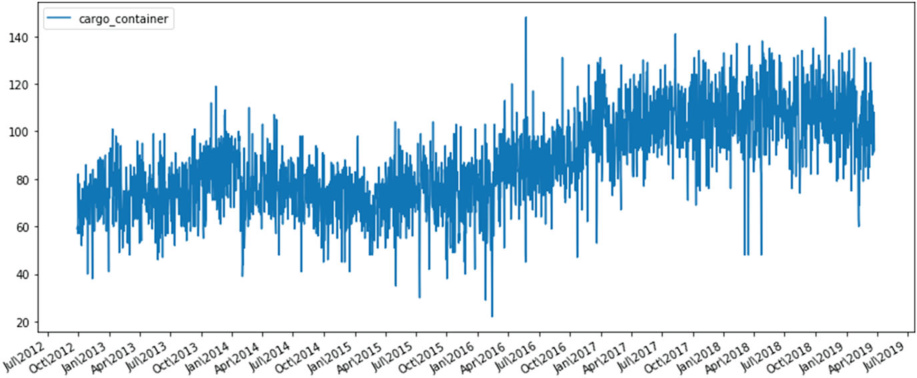
\includegraphics[width=0.8\textwidth]{gfx/m1l1_nowcast_cargo_container_index.jpg}
    \caption{Tổng số lượt cập bến của tàu container tại tất cả các cảng của Trung Quốc}
    \label{fig:nowcast_cargo_container_index}
\end{figure}

Để tránh sự biến động quá lớn trong dữ liệu hàng ngày, chúng tôi tính toán đường trung bình động (rolling average) trong 30 ngày của số lượng tàu thuộc ba loại đã chọn cập bến hàng ngày tại tất cả các cảng của Trung Quốc, như sau:
$$Ship_{(i,j)}^{q3}(t)=\frac{1}{30}\sum_{m=1}^{30}X_{i,j}(t-m)$$
với $X_{i,j}$ là số lượng tàu đến thuộc loại i [tàu container, tàu chở dầu, tàu chở hàng rời] tại một cảng j nhất định của Trung Quốc.

Cuối cùng, chúng tôi tính toán Chỉ số Thương mại Quốc tế QuantCube cho Trung Quốc sử dụng Phương trình (8) bằng cách cộng dồn ba loại hình vận chuyển và bằng cách tính toán những thay đổi so với cùng kỳ năm trước. Chỉ số này được thể hiện trong Hình 2. Chúng tôi nhận được mối tương quan là 80\% giữa Chỉ số Thương mại Quốc tế QuantCube theo thời gian thực và các con số thương mại chính thức của Trung Quốc (nhập khẩu + xuất khẩu). Đây là một chỉ số báo trước (leading index) 2 tháng do các con số chính thức về nhập khẩu và xuất khẩu hàng hóa được công bố với độ trễ 2 tháng sau khi kết thúc tháng tham chiếu. Chúng tôi nhận thấy chỉ báo của chúng ta chỉ ra rõ ràng tốc độ chậm lại của tổng thương mại Trung Quốc, chủ yếu bị tác động bởi số lượng gia tăng các lệnh trừng phạt thương mại của Mỹ kể từ giữa năm 2018.

\begin{figure}[htbp]
    \centering
    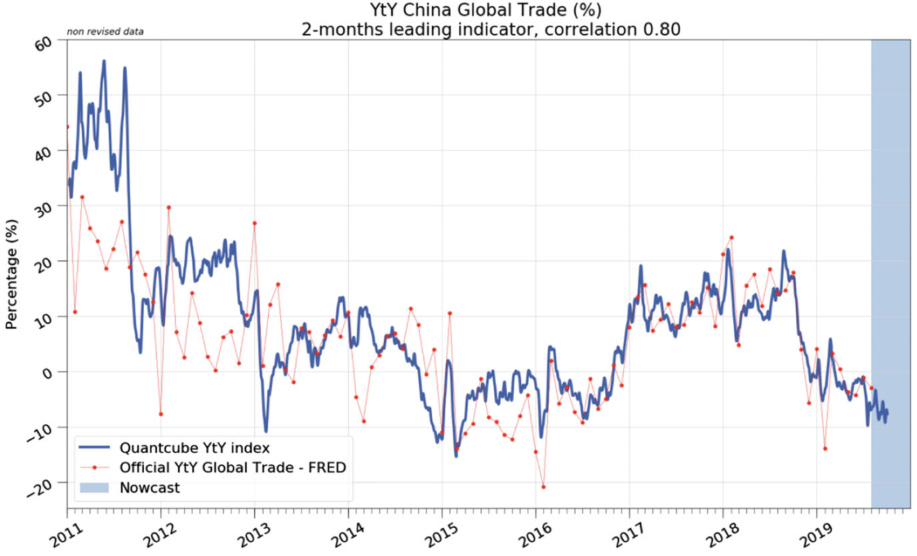
\includegraphics[width=0.8\textwidth]{gfx/m1l1_nowcast_china_trade_index.jpg}
    \caption{Chỉ số thương mại toàn cầu của Trung Quốc (tăng trưởng so với cùng kỳ năm trước tính bằng \%)}
    \label{fig:nowcast_china_trade_index}
\end{figure}

Đối với các quốc gia phụ thuộc nhiều vào các hoạt động trao đổi hàng hải, chỉ số này có thể đạt được mối tương quan với tổng các con số ngoại thương của quốc gia lên tới 95\%. Đối với các quốc gia chủ yếu dựa vào các giao dịch trên cạn, hóa ra chỉ số này vẫn là một biến đại diện tốt cho các trao đổi ở nước ngoài. Tuy nhiên, trong trường hợp sau, các biến đại diện của giao dịch qua đường hàng không và đường bộ có thể được tính toán để bổ sung thông tin, bằng cách sử dụng thông tin về các chuyến bay chở hàng hóa, phí cầu đường và lịch trình xe lửa.

\subsubsection{Một Biến đại diện Thời gian thực cho Tiêu dùng}

\paragraph{Tiêu dùng Cá nhân}
Khi theo dõi hoạt động kinh tế, tiêu dùng cá nhân (private consumption) là một tổng lượng vĩ mô quan trọng mà chúng ta cần đánh giá theo thời gian thực. Ví dụ, ở Mỹ, tiêu dùng cá nhân chiếm khoảng 70\% tăng trưởng GDP. Vì các con số chính thức về tiêu dùng cá nhân được công bố hàng tháng (ví dụ: ở Mỹ) hoặc hàng quý (ví dụ: ở Trung Quốc) và với độ trễ công bố từ 1 đến 3 tháng, các nguồn dữ liệu thay thế, chẳng hạn như Google Trends, có thể truyền tải thông tin hữu ích khi thiếu thông tin chính thức.

Vì chi tiêu cá nhân nằm trong các nhóm hàng hóa lâu bền, hàng hóa không lâu bền và dịch vụ, trước tiên chúng tôi tiến hành phân tích phương sai của tiêu dùng đối với các quốc gia được nghiên cứu, để làm nổi bật các thành phần chính của tiêu dùng mà chúng ta phải theo dõi. Ví dụ, đối với tiêu dùng của Trung Quốc, chúng tôi đã xác định các danh mục sau: Đồ xa xỉ (túi xách, đồng hồ, rượu vang, đồ trang sức), Bán lẻ (thực phẩm, đồ uống, quần áo, thuốc lá, điện thoại thông minh, máy tính, đồ điện tử), Phương tiện, Dịch vụ (khách sạn, khoản vay tín dụng, phương tiện đi lại) và Giải trí (du lịch, thể thao, điện ảnh, chơi game). Trong phần này, chúng tôi tập trung vào một chỉ số phụ (sub-indicator) của biến đại diện cho tiêu dùng Trung Quốc của QuantCube, đó là Du lịch (thuộc danh mục Giải trí). Phương pháp tương tự cũng được phát triển để theo dõi các thành phần chính khác của tiêu dùng hộ gia đình.

\paragraph{Nguồn Dữ liệu Thay thế}
Thành phần phụ du lịch của tiêu dùng Trung Quốc được cho là để theo dõi chi tiêu của người dân Trung Quốc cho các chuyến đi du lịch, trong và ngoài nước. Để tạo ra thành phần phụ này của chỉ số tiêu dùng, chúng tôi đã sử dụng các truy vấn tìm kiếm liên quan đến du lịch được trích xuất thông qua các ứng dụng Google Trends và Baidu. Trên thực tế, các truy vấn tìm kiếm trên Internet có sẵn thông qua Google Trends và Baidu cho phép chúng tôi xây dựng một biến đại diện (proxy) cho tiêu dùng cá nhân đối với các chuyến đi du lịch tại mỗi quốc gia vì các truy vấn tìm kiếm do khách du lịch thực hiện phản ánh xu hướng trong sở thích đi du lịch của họ, cũng như dự báo về điểm đến du lịch trong tương lai của họ. Google và Baidu Trends có các tính năng về xu hướng tìm kiếm cho thấy tần suất một cụm từ tìm kiếm cụ thể được nhập vào công cụ tìm kiếm của Google hoặc Baidu so với tổng khối lượng tìm kiếm của trang web trong một khoảng thời gian nhất định. Từ những truy vấn tìm kiếm này, chúng tôi đã xây dựng hai chỉ số khác nhau: số lượng khách du lịch trên mỗi điểm đến sử dụng bộ lọc khu vực "Tất cả các quốc gia" (All country) và số lượng khách du lịch từ một quốc gia cụ thể trên mỗi điểm đến bằng cách chọn quốc gia đó trong bộ lọc khu vực.

\paragraph{Chỉ số Du lịch Trung Quốc QuantCube}
Chỉ số Du lịch Trung Quốc QuantCube là một biến đại diện cho số lượng khách du lịch từ Trung Quốc đến mỗi điểm đến. Để tạo ra chỉ số này, trước tiên chúng tôi đã xác định 15 quốc gia được du khách Trung Quốc ghé thăm nhiều nhất, chiếm 60\% tổng lượng du khách Trung Quốc. Chúng tôi tạo một chỉ số du lịch của Trung Quốc cho từng quốc gia bằng cách xác định các danh mục liên quan dựa trên các khía cạnh khác nhau của việc lập kế hoạch chuyến đi, bao gồm phương tiện đi lại, các hoạt động du lịch, thời tiết, chỗ ở và mua sắm. Lấy ví dụ, để tạo ra Chỉ số du lịch Trung Quốc tại Hàn Quốc, chúng tôi đã xác định các danh mục liên quan sau: Du lịch Hàn Quốc, Visa Hàn Quốc, Bản đồ Hàn Quốc, Bản đồ Du lịch Hàn Quốc, Các điểm tham quan ở Hàn Quốc, Sân bay Seoul và Mua sắm ở Hàn Quốc (Hình 3).

\begin{figure}[htbp]
    \centering
    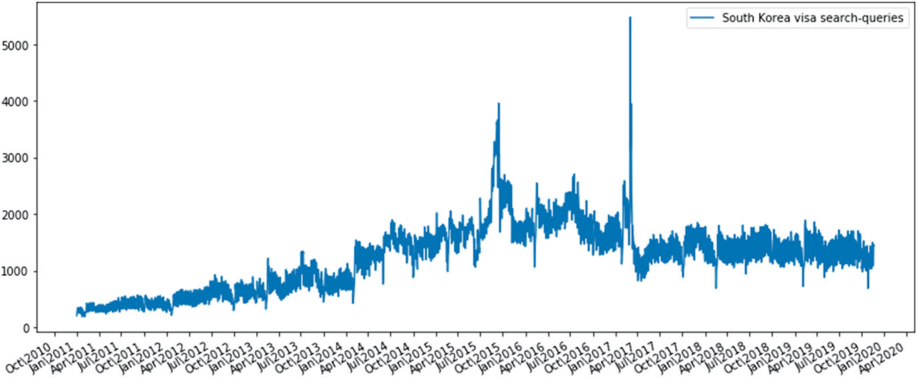
\includegraphics[width=0.8\textwidth]{gfx/m1l1_nowcast_korea_visa_searches.jpg}
    \caption{Baidu: Truy vấn tìm kiếm "Visa Hàn Quốc"}
    \label{fig:nowcast_korea_visa_searches}
\end{figure}

Cuối cùng, bằng cách tổng hợp các xu hướng truy vấn tìm kiếm của những từ khóa đã được xác định đó, Chỉ số Du lịch Trung Quốc tại Hàn Quốc của chúng tôi theo dõi theo thời gian thực sự phát triển của số liệu chính thức về lượng du khách Trung Quốc đến Hàn Quốc. Chúng tôi tính toán sự thay đổi so với cùng kỳ năm trước của chỉ số này và xác nhận nó bằng cách sử dụng các con số chính thức của khách du lịch Trung Quốc tại Hàn Quốc (xem Hình 4).

\begin{figure}[htbp]
    \centering
    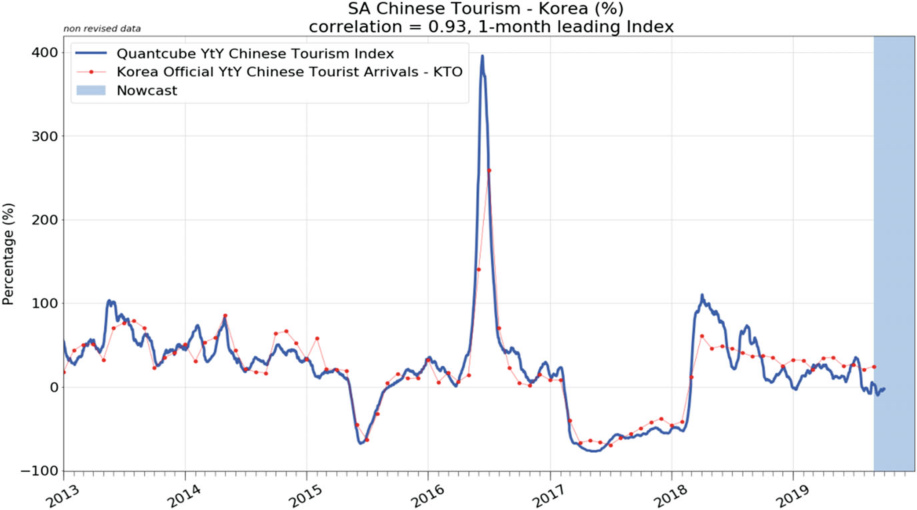
\includegraphics[width=0.8\textwidth]{gfx/m1l1_nowcast_chinese_tourism_korea.jpg}
    \caption{Chỉ số du lịch Trung Quốc tại Hàn Quốc ngắn hạn (so với cùng kỳ năm trước tính bằng \%)}
    \label{fig:nowcast_chinese_tourism_korea}
\end{figure}

Từ Hình 4, chúng ta quan sát thấy rằng Chỉ số Du lịch Trung Quốc QuantCube theo dõi chính xác lượng du khách Trung Quốc đến Hàn Quốc. Ví dụ, chỉ số này đã nắm bắt được sự sụt giảm đầu tiên vào tháng 6 năm 2015 do đợt bùng phát MERS. Hơn nữa, vào năm 2017, sau thông báo về việc lắp đặt Hệ thống phòng thủ khu vực tầm cao giai đoạn cuối (THAAD) hùng mạnh vào cuối năm 2016, chính phủ Trung Quốc đã cấm các nhóm du lịch đến Hàn Quốc như một sự trả đũa kinh tế. Trong toàn bộ năm 2017, Hàn Quốc có 4,2 triệu du khách Trung Quốc – giảm 48,3\% so với năm trước. Sự sụt giảm của khách du lịch Trung Quốc dẫn đến việc lượng khách du lịch nhập cảnh giảm 36\%. Do đó, chỉ báo Du lịch Trung Quốc thời gian thực này cũng rất hữu ích để ước tính trong thời gian thực xu hướng của ngành Du lịch Hàn Quốc. Nó theo dõi lượng du khách Trung Quốc đến với mức tương quan lên đến 95\%.

Cuối cùng, chúng tôi đã phát triển các chỉ số tương tự để theo dõi theo thời gian thực lượng du khách Trung Quốc đến 15 quốc gia được ghé thăm nhiều nhất (Mỹ, Châu Âu, v.v.); chúng tôi nhận được mối tương quan trung bình là 80\% cho các quốc gia được ghé thăm nhiều nhất. Bằng cách tổng hợp các chỉ số đó, chúng tôi có thể xây dựng một chỉ số để theo dõi lượng du khách Trung Quốc trên toàn thế giới, cung cấp một biến đại diện (proxy) tuyệt vời cho chi tiêu của các hộ gia đình Trung Quốc trong lĩnh vực cụ thể này.

\subsubsection{Một Biến đại diện Thời gian thực cho Mức độ Hoạt động}

QuantCube Technology đã phát triển một phương pháp luận dựa trên việc phân tích các hình ảnh vệ tinh Sentinel-2 để phát hiện các cơ sở hạ tầng mới (thương mại, hậu cần, công nghiệp hoặc khu dân cư) và đo lường sự tiến hóa về hình dạng và kích thước của các khu vực đô thị. Tuy nhiên, mức độ hoạt động hoặc mức độ khai thác của các khu vực này khó có thể được xác định bằng cách kiểm tra tòa nhà mà có thể được suy luận từ sự hiện diện của các phương tiện từ các đường phố và bãi đậu xe gần đó. Với mục đích này, QuantCube Technology hợp tác với IRISA đã phát triển một mô hình học sâu (deep learning) để đếm xe cộ từ các hình ảnh vệ tinh lấy từ cảm biến Pleiades ở độ phân giải không gian 50 cm. Trên thực tế, chúng tôi chọn vệ tinh tùy thuộc vào độ phân giải pixel cần thiết cho mỗi ứng dụng.

\paragraph{Hình ảnh Vệ tinh}
Hình ảnh vệ tinh ngày càng trở nên dễ tiếp cận hơn trong những năm gần đây. Đặc biệt, một số vệ tinh công cộng cung cấp khả năng truy cập dễ dàng và miễn phí vào kho lưu trữ hình ảnh của họ, với độ phân giải không gian đủ cao cho nhiều ứng dụng liên quan đến đặc tính đất đai. Ví dụ, dòng vệ tinh Sentinel-2 của Cơ quan Vũ trụ Châu Âu (ESA), được phóng vào ngày 23 tháng 6 năm 2015, cung cấp các hình ảnh đa phổ độ phân giải 10 mét bao phủ toàn thế giới. Chúng tôi phân tích những hình ảnh này để phát hiện cơ sở hạ tầng. Để phát hiện và đếm ô tô, chúng tôi sử dụng hình ảnh VHR (độ phân giải rất cao - very high resolution) có độ phân giải cao hơn thu được từ vệ tinh Pleiades (PHR-1A và PHR-1B), do Cơ quan Vũ trụ Pháp (CNES), Phân phối Airbus DS phóng. Những hình ảnh này là các sản phẩm được làm sắc nét toàn sắc (pan-sharpened) thu được bằng cách kết hợp dữ liệu toàn sắc (panchromatic) 50 cm (70 cm ở thiên để, được lấy mẫu lại ở mức 50 cm) và hình ảnh đa phổ 2 m (RGB khả kiến (đỏ, lục, lam) và các dải hồng ngoại). Chúng bao phủ một khu vực lớn gồm các môi trường không đồng nhất bao gồm nông thôn, rừng, khu dân cư, cũng như các khu công nghiệp, nơi sự xuất hiện của các phương tiện bị ảnh hưởng bởi hiệu ứng đổ bóng và che khuất. Một mặt, một trong những ưu điểm của các ứng dụng dựa trên hình ảnh vệ tinh là khả năng mở rộng thế giới tự nhiên (natural world scalability) của chúng. Và mặt khác, sự tiến hóa và cải tiến của các thuật toán trí tuệ nhân tạo cho phép chúng ta xử lý một lượng lớn thông tin có trong hình ảnh vệ tinh một cách dễ dàng, mang lại một giải pháp chuẩn hóa và tự động hoạt động trên dữ liệu thời gian thực.

\paragraph{Tiền xử lý và Lập mô hình}
Việc phát hiện phương tiện từ hình ảnh vệ tinh là một trường hợp đặc biệt của phát hiện đối tượng vì các đối tượng có tính đồng nhất và rất nhỏ (khoảng 5 đến 8 pixel/phương tiện trong hình ảnh Pleiades) và không xếp chồng lên nhau. Để giải quyết nhiệm vụ này, chúng tôi sử dụng một mô hình có tên là Tiramisu 100 lớp (xem [40]). Đây là một mô hình khá tiết kiệm vì nó chỉ có 9 triệu tham số, so với khoảng 130 triệu của mạng học sâu sơ khai được gọi là VGG19. Mục tiêu của mô hình là khai thác việc tái sử dụng tính năng bằng cách mở rộng kiến trúc DenseNet trong khi tránh sự bùng nổ tính năng (feature explosion). Để huấn luyện mô hình học sâu của chúng tôi, chúng tôi đã tạo một tập dữ liệu huấn luyện bằng cách sử dụng công cụ gán nhãn tương tác cho phép gán nhãn 60\% số lượng phương tiện chỉ bằng một cú nhấp chuột sử dụng các phương pháp flood-fill được điều chỉnh cho ứng dụng này. Tập dữ liệu được tạo chứa 87.000 phương tiện được chú thích từ các môi trường khác nhau tùy thuộc vào mức độ đô thị hóa. Từ việc phân đoạn, ước tính về số lượng phương tiện được tính toán dựa trên kích thước và hình dạng của các dự đoán.

\paragraph{Chỉ số Mức độ Hoạt động QuantCube}
Cuối cùng, mô hình thực hiện một dự đoán thỏa mãn đối với ứng dụng phát hiện và đếm phương tiện vì độ chính xác (precision) đạt hơn 85\% trên tập xác thực (validation set) gồm 2673 phương tiện thuộc các khu đô thị và công nghiệp. Thuật toán hiện tại có khả năng xử lý các môi trường đô thị khác nhau. Như có thể thấy trong Hình 5, hiển thị toàn cảnh khu vực Orly gần Paris, bao gồm dự đoán về việc phát hiện và đếm xe ô tô bằng màu vàng, mã có khả năng đếm chính xác số lượng phương tiện ở một số khu vực được xác định. Ví dụ trong Hình 5 cho thấy số lượng phương tiện cho mỗi hộp giới hạn (bounding box) được xác định tương ứng với bãi đậu xe của các địa điểm khách sạn, thương mại hoặc hậu cần (logistics). Bắt đầu từ thông tin dựa trên vệ tinh này, chúng tôi có thể tính toán một chỉ số để phát hiện và đếm số lượng phương tiện ở các địa điểm được xác định và để theo dõi mức độ hoạt động hoặc mức độ khai thác của chúng bằng cách xem xét sự phát triển của chỉ số tương quan với các chỉ số bán hàng. Sử dụng hình ảnh vệ tinh, nó cho phép tạo ra một phương pháp luận và các thước đo chuẩn hóa về mức độ hoạt động cho phép các tổ chức tài chính và các nhóm công ty dự đoán các xu hướng đầu tư mới trước khi công bố các con số kinh tế chính thức.

\begin{figure}[htbp]
    \centering
    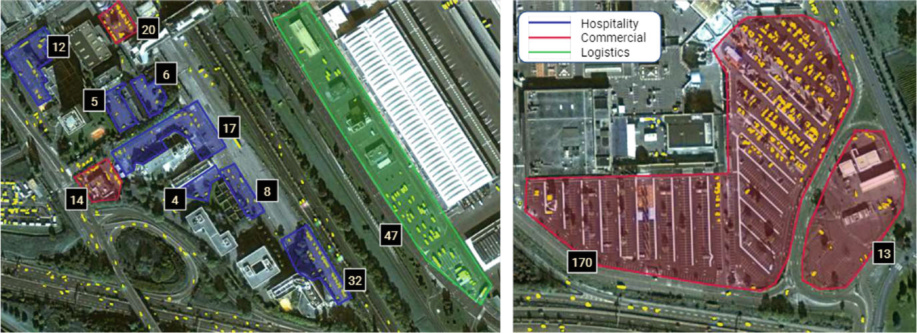
\includegraphics[width=0.8\textwidth]{gfx/m1l1_nowcast_satellite_parking.jpg}
    \caption{Số lượng xe theo từng khu vực ở Orly}
    \label{fig:nowcast_satellite_parking}
\end{figure}



% ---- Lesson 2: Government Data ----
% Thứ tự đọc: Lesson Notes (trong VM, xem ghi chú trong chương) -> Đọc thêm
\chapter{Dữ liệu chính phủ}
\label{ch:M1L2}

\section*{Lesson Notes}
\section[Dữ liệu Kinh tế và Tài chính]{Dữ liệu Kinh tế và Tài chính (Economics and Financial Data)}

Giá cả tài sản bị ảnh hưởng rất lớn bởi những gì diễn ra trong nền kinh tế vĩ mô. Một chu kỳ kinh doanh bùng nổ sẽ thu hút đầu tư vốn cổ phần, làm tăng chi tiêu cá nhân, và có thể dẫn đến các hành động từ ngân hàng trung ương. Trong module đầu tiên về Thị trường Tài chính, bạn đã thấy các ví dụ trong đó người gửi tiền hưởng một mức lãi suất cụ thể. Cùng lúc đó, người cho vay (hoặc người đi vay) lại chịu một mức lãi suất khác. Gửi tiền vào ngân hàng chắc chắn sẽ mang lại mức tiền lãi thấp hơn so với tiền lãi bạn phải trả cho một khoản vay từ chính ngân hàng đó!

Một trong những yếu tố ảnh hưởng lớn nhất đến thị trường nói chung, và lãi suất nói riêng, là tin tức. Tin tức có thể được coi là nằm trong dự kiến (expected) hoặc ngoài dự kiến (unexpected). Hãy nhớ lại rằng các thị trường hiệu quả có thể đã phản ánh phần lớn các tin tức dự kiến vào giá. Ví dụ, giả sử Netflix tuyên bố trả cổ tức \$2.00. Nếu đây thực sự là con số được công bố, thì nó không gây ngạc nhiên và sẽ không ảnh hưởng đến giá cổ phiếu của Netflix. Tuy nhiên, giả sử có tin tức ngoài dự kiến.

\begin{itemize}
    \item Netflix có sự tăng trưởng mạnh hơn dự đoán do đánh giá thấp mức độ phổ biến của một số chương trình, dẫn đến số lượng người đăng ký tại Hàn Quốc lớn hơn dự kiến. Mức cổ tức là \$2.40. Giá cổ phiếu có khả năng sẽ tăng vọt.
    \item Mặt khác, giả sử Netflix có chi phí sản xuất nội dung gốc cao hơn dự kiến, khiến lợi nhuận ròng sụt giảm. Cổ tức chỉ còn \$1.80. Giá cổ phiếu có khả năng sẽ lao dốc.
\end{itemize}

Tin tức ngoài dự kiến có thể là tin tốt hoặc tin xấu; tức là, nó có thể dẫn đến giá cao hơn hoặc giá thấp hơn, tùy thuộc vào tình hình. Ví dụ, hãy xem xét tin xấu. Nó có thể làm tăng rủi ro tín dụng, đe dọa dòng tiền tài trợ, tạo ra sự biến động, phá vỡ mối tương quan, làm trầm trọng thêm đòn bẩy, gây ra tính phi tuyến, thách thức các giả định của mô hình, gây áp lực lên các mô hình bằng cách phát sinh thêm chi phí cho thanh khoản, thúc đẩy sự thất bại của mô hình, và thậm chí mang lại các cuộc khủng hoảng tài chính. Tất nhiên, một mẩu tin xấu có thể không gây ra tất cả những điều đó, nhưng sẽ ra sao nếu tin xấu ảnh hưởng đến nhiều doanh nghiệp, chẳng hạn như lãi suất cao hơn dự kiến?

Hãy xem xét cách thức hoạt động của lãi suất. Đầu tư vào kinh doanh ảnh hưởng đến lãi suất, nhưng đồng thời, lãi suất cũng ảnh hưởng đến các khoản đầu tư kinh doanh. Hầu hết các mối quan hệ trong tài chính đều phức tạp vì chúng có thể mang tính đa chiều. Không chỉ là A ảnh hưởng đến B và B ảnh hưởng đến A. Mà là A ảnh hưởng đến B và C; B ảnh hưởng đến A và C; C ảnh hưởng đến A và B; và cứ tiếp tục như vậy. Ví dụ, nếu chúng ta chỉ thu thập lãi suất mà không có ý niệm gì về chính sách tiền tệ, cung tiền hay các quyết định kinh tế, chúng ta sẽ đánh mất đi dữ liệu mà vừa ảnh hưởng đến lãi suất lại vừa bị ảnh hưởng bởi chính các mức lãi suất đó. Thực tế, chúng ta có thể muốn thu thập các dữ liệu liên quan để có thể kiểm tra xem các biến số khác (ví dụ: các quyết định của Fed) có ảnh hưởng đến biến số mà chúng ta đang quan tâm hay không.

\section[Cục Dự trữ Liên bang và Tác động của nó]{Cục Dự trữ Liên bang và Tác động của nó (The Federal Reserve and Its Impact)}

Nhớ lại từ môn Thị trường Tài chính rằng chúng ta đã đọc về các ngân hàng trung ương. Cục Dự trữ Liên bang (Federal Reserve - Fed) là ngân hàng trung ương của Hoa Kỳ. Đầu ra của Fed rất rộng lớn: nó bao gồm các quyết định, nghiên cứu, và các bài bình luận thị trường được xuất bản và phát biểu. Những kết quả này được theo dõi và phân tích rất kỹ lưỡng, vì chúng ảnh hưởng đáng kể đến thị trường. Ví dụ, tám lần một năm, Cục Dự trữ Liên bang có lịch trình phát hành thường xuyên các quyết định về lãi suất. Những cuộc họp này dẫn đến các quyết định về lãi suất được công bố ra thị trường. Giống như bất kỳ thông tin nào khác, đây là tin tức có thể nằm trong dự kiến hoặc ngoài dự kiến. Nếu tin tức là trong dự kiến, thì thông tin đó đã được phản ánh vào giá trên thị trường. Nếu tin tức là ngoài dự kiến, thì rất có khả năng sẽ có những cú sốc thông tin gây ra sự biến động trên thị trường. Ngoài ra, Fed còn chọn 8 ngày khác để công bố biên bản các cuộc họp. Những bản phát hành này chứa dữ liệu định tính thay vì định lượng. Các bản công bố này cũng có thể ảnh hưởng không chỉ đến lãi suất mà còn đến giao dịch chứng khoán, vì chúng chỉ ra ý kiến và hành động dự kiến của Fed. Ví dụ, vào năm 2019, Fed đã quyết định cắt giảm lãi suất ba lần. Điều này đã dẫn đến mức tăng 29\% của chỉ số S\&P 500 trong quý 4 năm 2019.

Nếu chúng ta thu thập dữ liệu trong năm 2018 và sau đó cố gắng ngoại suy, chúng ta sẽ bỏ lỡ các sự kiện chính ảnh hưởng đến dữ liệu. Thường thì, chúng ta cần phải hiểu các sự kiện chính tác động đến dữ liệu của mình, vì chúng ta có thể coi một mẫu dữ liệu là thông tin giữa các sự kiện đó. Ví dụ, nếu bạn xây dựng một mẫu dữ liệu vốn cổ phần, bạn có thể thu thập giá đóng cửa của cổ phiếu hàng ngày, nhưng khi tiến hành phân tích chúng, bạn có thể xem xét:
\begin{enumerate}
    \item không phân nhóm
    \item 1 nhóm cho mỗi lần thông báo cổ tức của cổ phiếu
    \item phân nhóm dựa trên mức lãi suất của Cục Dự trữ Liên bang
    \item 1 nhóm cho mỗi cuộc họp quỹ Fed
\end{enumerate}

Mặc dù dữ liệu thu thập được có thể giống nhau, nhưng có một sự thừa nhận rằng toàn bộ dữ liệu (ví dụ 1) có thể có các đặc tính khác nhau và có thể được phân tích tốt hơn dựa trên thuộc tính nội tại của công ty (ví dụ 2, thu nhập) hoặc dựa trên thuộc tính bên ngoài, như chính sách tiền tệ (ví dụ 3 và 4). Hiểu được rằng dữ liệu của chúng ta trải qua sự thay đổi đồng nghĩa với việc chúng ta sẽ muốn hiểu các thị trường như những hệ thống. Điều đó cũng có nghĩa là chúng ta có thể muốn thu thập và phân tích các dữ liệu mang tính định tính (ví dụ: các tuyên bố của Fed).

\section[Dữ liệu Chính phủ là gì?]{Dữ liệu Chính phủ là gì? (What is Government Data?)}

Dữ liệu chính phủ là tất cả những thông tin được thu thập bởi các thực thể chính phủ. Dữ liệu này bao gồm:
\begin{itemize}
    \item Dữ liệu Kinh tế (GDP, lạm phát, tỷ lệ việc làm, v.v.)
    \item Dữ liệu Nhân khẩu học
    \item Dữ liệu Môi trường
    \item Dữ liệu Y tế
    \item Dữ liệu Pháp lý
    \item Dữ liệu Nông nghiệp
    \item Dữ liệu Năng lượng
    \item Dữ liệu Giáo dục
    \item Dữ liệu Bất động sản
\end{itemize}

và nhiều danh mục dữ liệu khác mà một chính phủ cụ thể có thể chọn hoặc không chọn để theo dõi. Dữ liệu trên là rất cần thiết cho mọi cơ chế ra quyết định được chính phủ kết hợp. Ví dụ, đã được xác định rõ dữ liệu kinh tế quan trọng như thế nào đối với chính sách tiền tệ và tài khóa hay dữ liệu y tế đã giúp các cơ quan tương ứng điều phối phản ứng của hệ thống chăm sóc sức khỏe trong đại dịch COVID-19 ra sao.

Về bản chất, dữ liệu này đóng vai trò như sự quản trị dựa trên bằng chứng và cái nhìn toàn diện của chúng cho phép các chính phủ đưa ra các quyết định cho tương lai của một quốc gia trong bối cảnh thực tế phức tạp.

\subsection[Các khía cạnh của Dữ liệu Chính phủ]{Các khía cạnh của Dữ liệu Chính phủ (Aspects of Government Data)}

Tính đến lúc này, chúng ta đã thấy phạm vi của dữ liệu chính phủ, nhưng cũng có những đặc điểm khác:
\begin{itemize}
    \item Khối lượng (Volume): khối lượng dữ liệu chính phủ có xu hướng rất lớn
    \item Đa dạng (Variety): nhiều danh mục dữ liệu có cấu trúc và phi cấu trúc
    \item Thẩm quyền (Authoritative): nó mang tính chính thức (cùng một dữ liệu được sử dụng để hoạch định chính sách)
    \item Tính kịp thời (Timeliness): người ta có thể tìm thấy dữ liệu thời gian thực và dữ liệu lịch sử
    \item Chất lượng (Quality): có thể có những tập dữ liệu không đầy đủ hoặc không chính xác
    \item Định dạng (Format): dữ liệu được lưu trong cơ sở dữ liệu, các tệp (CSV, JSON, v.v.), báo cáo, và các định dạng khác
    \item Độ nhạy cảm/Khả năng tiếp cận (Sensitivity/Accessibility): nó có thể bao gồm thông tin cá nhân, trong trường hợp đó nó sẽ bị hạn chế
    \item Siêu dữ liệu (Metadata): các mô tả của tập dữ liệu đóng vai trò như một bản kiểm kê để điều hướng khối lượng dữ liệu lớn
\end{itemize}

Bổ sung thêm, liên quan đến các đặc điểm trên, đã có một nỗ lực đáng kể từ phía một số chính phủ nhằm thực hiện tính minh bạch và tính mở trong dữ liệu của họ. Những nỗ lực này đã làm nảy sinh Dữ liệu Chính phủ Mở (Open Government Data), mang hình thức của một phong trào thúc đẩy nhiều quốc gia cung cấp quyền truy cập công khai vào dữ liệu của họ.

\subsection[Dữ liệu Chính phủ Mở]{Dữ liệu Chính phủ Mở (Open Government Data)}

Năm 1966, Hoa Kỳ là nước đầu tiên thực hiện chính sách về dữ liệu mở bằng cách thiết lập một khuôn khổ pháp lý mang tên "Đạo luật Tự do Thông tin" (Freedom of Information Act - FOIA). Theo FOIA, bất kỳ công dân nào cũng có thể yêu cầu quyền truy cập công khai vào các hồ sơ từ bất kỳ cơ quan liên bang nào. Nhưng đây là tính minh bạch mang tính "phản ứng" (reactive) vì dữ liệu không được mở theo mặc định. Điều này chỉ được sửa đổi vào năm 2009 bởi Chỉ thị Chính phủ Mở (Open Government Directive), bắt buộc các cơ quan liên bang phải xuất bản thông tin chính phủ trực tuyến và đi theo chính sách chính phủ mở. Đây là bước đi quyết định từ tính minh bạch "phản ứng" sang tính minh bạch "chủ động" (proactive), nơi bất kỳ ai cũng có thể truy cập dữ liệu công cộng mà không cần phải có yêu cầu rõ ràng. Vương quốc Anh cũng ra mắt Sáng kiến Dữ liệu Mở vào năm 2010, tiếp theo là Chỉ thị Dữ liệu Mở của EU vào năm 2019. Các quốc gia khác như Canada, Úc, Ấn Độ và Nhật Bản cũng đã thực hiện các chính sách dữ liệu mở của riêng họ.

Dưới đây là định nghĩa về Dữ liệu Chính phủ Mở như được tìm thấy trong Cổng Dữ liệu Châu Âu (European Data Portal):

Dữ liệu (Chính phủ) Mở đề cập đến thông tin được thu thập, sản xuất hoặc được chi trả bởi các cơ quan công quyền (còn được gọi là Thông tin Khu vực Công) và được cung cấp miễn phí để tái sử dụng cho bất kỳ mục đích nào. Giấy phép sẽ chỉ định rõ các điều khoản sử dụng. Những nguyên tắc đối với Dữ liệu Mở này được mô tả chi tiết trong Định nghĩa Mở (Open Definition).

Tập con này của dữ liệu chính phủ sẽ (một phần) định hướng các tập dữ liệu mà bạn sẽ sử dụng tại WQU. Những tập dữ liệu trong thế giới thực này sẽ giúp bạn phát triển các kỹ năng thực tế trong việc phân tích và lập mô hình dữ liệu, đồng thời mang lại cái nhìn sâu sắc về các chỉ số kinh tế và các yếu tố khác ảnh hưởng đến nền kinh tế. Tóm lại, tính minh bạch trong dữ liệu chính phủ đã làm phong phú thêm nội dung của WQU cũng như toàn bộ quá trình học tập.

\subsection[Dữ liệu Kinh tế của Cục Dự trữ Liên bang]{Dữ liệu Kinh tế của Cục Dự trữ Liên bang (Federal Reserve Economic Data - FRED)}

Một ví dụ điển hình về dữ liệu chính phủ mở đang hoạt động là Dữ liệu Kinh tế của Cục Dự trữ Liên bang (FRED). Hiện tại, FRED nổi bật với tư cách là một trong những cơ sở dữ liệu kinh tế toàn diện và dễ tiếp cận nhất dành cho công chúng. Dữ liệu này được duy trì bởi Ngân hàng Dự trữ Liên bang St. Louis và được đặc biệt quan tâm, phù hợp với các nguyên tắc về tính mở, như một nguồn tài nguyên quan trọng cho các nhà nghiên cứu, các nhà hoạch định chính sách, sinh viên và công chúng.

\subsubsection[Tổng quan về FRED]{Tổng quan về FRED (Overview of FRED)}

FRED là một kho lưu trữ khổng lồ về dữ liệu chuỗi thời gian kinh tế từ nhiều nguồn khác nhau, không chỉ giới hạn trong Hệ thống Dự trữ Liên bang. Nó bao gồm dữ liệu từ:
\begin{itemize}
    \item Các cơ quan chính phủ Hoa Kỳ (ví dụ: Cục Thống kê Lao động, Cục Phân tích Kinh tế)
    \item Các tổ chức quốc tế (ví dụ: Ngân hàng Thế giới, OECD)
    \item Các nguồn tư nhân (ví dụ: các trung tâm nghiên cứu của trường đại học)
\end{itemize}

Cơ sở dữ liệu bao gồm một loạt các chỉ số kinh tế, bao gồm:
\begin{itemize}
    \item Tổng sản phẩm quốc nội (GDP)
    \item Tỷ lệ lạm phát
    \item Thống kê việc làm
    \item Lãi suất
    \item Tỷ giá hối đoái
    \item Chỉ số giá tiêu dùng và nhà sản xuất
    \item Các khối tiền tệ (Monetary aggregates)
\end{itemize}

\subsubsection[Các tính năng chính của FRED]{Các tính năng chính của FRED (Key Features of FRED)}

1. Khả năng tiếp cận: Dữ liệu FRED được cung cấp miễn phí thông qua giao diện web thân thiện với người dùng, các ứng dụng di động và truy cập API.
2. Trực quan hóa Dữ liệu: Người dùng có thể tạo biểu đồ và đồ thị tùy chỉnh trực tiếp trên trang web FRED.
3. Tải xuống Dữ liệu: Dữ liệu có thể dễ dàng được tải xuống dưới nhiều định dạng (ví dụ: Excel, CSV) để phân tích thêm.
4. Cập nhật Thường xuyên: FRED được cập nhật theo thời gian thực khi có dữ liệu mới từ các nguồn của nó.
5. Dữ liệu Lịch sử: Nhiều chuỗi trong FRED có dữ liệu lùi lại vài thập kỷ, cung cấp bối cảnh lịch sử có giá trị.
6. Chuyển đổi Dữ liệu: FRED cho phép người dùng thực hiện các chuyển đổi cơ bản trên các chuỗi dữ liệu, chẳng hạn như thay đổi đơn vị hoặc tính toán phần trăm thay đổi.

Cho mục đích của bài học này, chúng ta sử dụng cổng API để có thể sử dụng các thư viện thống kê và trực quan hóa của Python.

\section[Đường cong Lợi suất]{Đường cong Lợi suất (Yield Curve)}

Trong phần này, chúng ta sẽ làm việc với một loại đường cong lợi suất cụ thể gọi là đường cong lợi suất Trái phiếu Kho bạc Kỳ hạn Không đổi (Constant Maturity Treasury - CMT). Trong môn Thị trường Tài chính, sinh viên đã được giới thiệu về chủ đề này, và chúng ta sẽ bổ sung cho tài liệu đó bằng một quy trình làm việc với dữ liệu thực hành.

Đường cong lợi suất CMT là một bức ảnh chụp nhanh về tất cả lợi suất Trái phiếu Kho bạc Hoa Kỳ tại một ngày nhất định. Về cơ bản, Bộ Tài chính Hoa Kỳ sử dụng lợi suất chào mua trên thị trường lúc đóng cửa (dựa trên mức giá mà người mua sẵn sàng trả (bid) thay vì giá giao dịch thực tế) để tính toán các mức lãi suất CMT hàng ngày. Bạn có thể tìm thấy tổng quan về phương pháp luận mà Bộ Tài chính sử dụng tại đây.

Một cách thuận tiện, FRED đã thực hiện các tính toán này và lãi suất CMT được cung cấp miễn phí từ trang web của họ hoặc thông qua FRED API, mà chúng ta có thể tận dụng thông qua thư viện Python \texttt{fredapi}. Để truy cập dữ liệu FRED, mỗi sinh viên phải lấy một khóa API (API key) bằng cách làm theo các bước sau:
1. Truy cập trang web FRED: https://fred.stlouisfed.org/docs/api/api\_key.html. Nhấp vào "Create an Account" (Tạo tài khoản) ở góc trên cùng bên phải (nếu bạn chưa có tài khoản với FRED).
2. Đăng nhập vào tài khoản FRED của bạn và yêu cầu khóa API. Điều hướng đến mục "API Keys" của menu thả xuống "My Account" ở góc trên cùng bên phải. Sau đó, nhấp vào "Request API Key."

\begin{lstlisting}[language=Python]
In [1]: import pandas as pd
        from fredapi import Fred
        import matplotlib.pyplot as plt
        import seaborn as sns
        sns.set()
\end{lstlisting}

\begin{lstlisting}[language=Python]
In [2]: # Initialize the FRED API with your key
        fred = Fred(api_key='99b15e0a2f3b3f4571893e831fd555d0') # Replace my APIKEY
        
        # List of Treasury yield series IDs
        series_ids = ['DGS1MO', 'DGS3MO', 'DGS6MO', 'DGS1', 'DGS2', 'DGS3', 'DGS5', 
                      'DGS7', 'DGS10', 'DGS20', 'DGS30']
        
        # Function to get data for a single series
        def get_yield_data(series_id):
            data = fred.get_series(series_id, observation_start="1975-01-01", observ
            return data
            
        #Get data for all series
        yields_dict = {series_id: get_yield_data(series_id) for series_id in series_
        
        # Combine into a single DataFrame
        yields = pd.DataFrame(yields_dict)
        
        # Rename columns for clarity
        yields.columns = ['1 Month', '3 Month', '6 Month', '1 Year', '2 Year', '3 Ye
                          '7 Year', '10 Year', '20 Year', '30 Year']
\end{lstlisting}

\begin{lstlisting}[language=Python]
In [3]: yields.index = pd.to_datetime(yields.index)
        yields.loc['2020-01-03']
\end{lstlisting}

\begin{lstlisting}[language=Python]
Out [3]: 1 Month    1.52
         3 Month    1.52
         6 Month    1.55
         1 Year     1.55
         2 Year     1.53
         3 Year     1.54
         5 Year     1.59
         7 Year     1.71
         10 Year    1.80
         20 Year    2.11
         30 Year    2.26
         Name: 2020-01-03 00:00:00, dtype: float64
\end{lstlisting}

Dataframe trên chứa một hàng từ bộ dữ liệu của chúng ta: tất cả các lợi suất CMT tại một ngày cụ thể.
Các mức lợi suất được biểu thị dưới dạng phần trăm. Ví dụ, lợi suất "1 Month" là 1.52, có nghĩa là 1.52\% hoặc 0.0152, và độ chính xác của các mức lợi suất được trình bày là một điểm cơ bản (0.01\%).

\begin{lstlisting}[language=Python]
In [4]: yields.isna().sum(axis = 0)
\end{lstlisting}

\begin{lstlisting}[language=Python]
Out [4]: 1 Month    7180
         3 Month    2204
         6 Month    2204
         1 Year      542
         2 Year      894
         3 Year      542
         5 Year      542
         7 Year      542
         10 Year     542
         20 Year    2231
         30 Year    1072
         dtype: int64
\end{lstlisting}

Điều đầu tiên chúng ta nhận thấy là phần dữ liệu bị thiếu. Một số kỳ hạn như 1 tháng, 3 tháng và 6 tháng không được theo dõi qua thời gian vì trước những năm 2000, trọng tâm chủ yếu nằm ở các kỳ hạn dài hơn. Trái phiếu 20 năm có lịch sử phát hành không đều đặn vì từ năm 1986 đến 1993, T-bonds 20 năm không được phát hành. Điều tương tự cũng áp dụng cho kỳ hạn 30 năm, vốn đã bị ngừng từ tháng 2 năm 2002 đến tháng 2 năm 2006. Hơn nữa, một lượng lớn các giá trị bị thiếu, như ta có thể thấy ở các trái phiếu có tính thanh khoản cao hơn như kỳ hạn 3, 5, 7 và 10 năm, có thể là do các ngày nghỉ lễ và sự gián đoạn của thị trường.

\begin{lstlisting}[language=Python]
In [5]: # We can see that during the days that the 10-year is not reported,
        # none maturity is reported as well.
        yields[yields['10 Year'].isna() == True].sum(axis = 0)
\end{lstlisting}

\begin{lstlisting}[language=Python]
Out [5]: 1 Month    0.0
         3 Month    0.0
         6 Month    0.0
         1 Year     0.0
         2 Year     0.0
         3 Year     0.0
         5 Year     0.0
         7 Year     0.0
         10 Year    0.0
         20 Year    0.0
         30 Year    0.0
         dtype: float64
\end{lstlisting}

Hãy vẽ biểu đồ lợi suất cho tất cả các ngày khả dụng. Mặc dù bộ dữ liệu của chúng ta chỉ trở nên "hoàn chỉnh" sau những năm 2000, việc quan sát cách lãi suất tiến triển qua thời gian vẫn rất quan trọng.

\begin{lstlisting}[language=Python]
In [6]: # Figure 1
        yields.plot(figsize=(12,8), title='Treasury Yields', alpha=0.7) # Plot the 
        plt.show()
\end{lstlisting}

\begin{figure}[htbp]
    \centering
    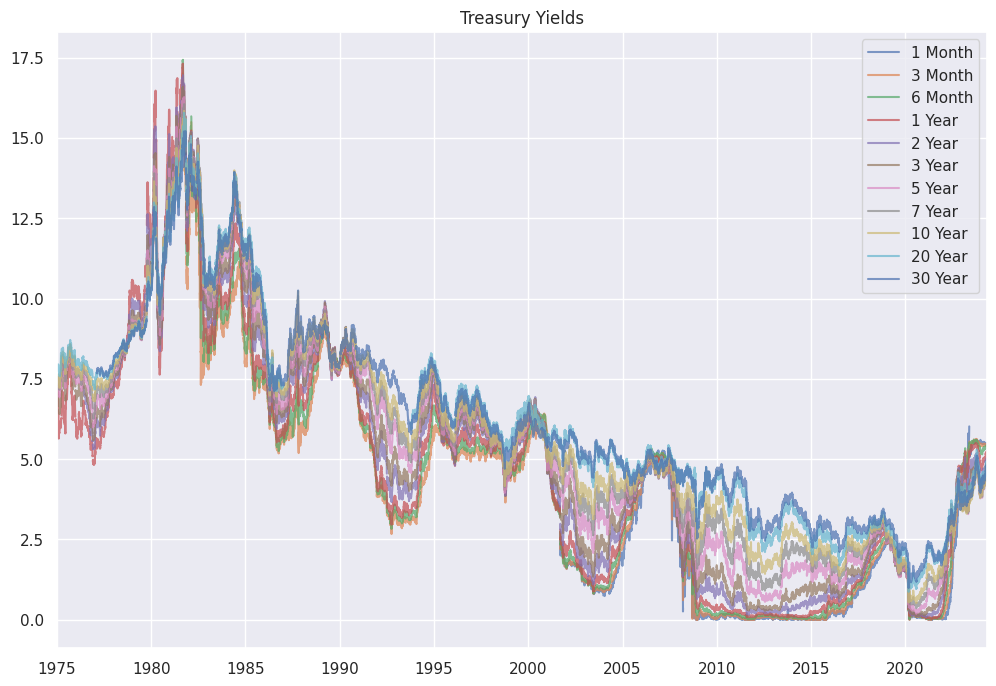
\includegraphics[width=1\textwidth]{gfx/m1l2_notes_fig1_treasury_yields.png}
    \caption{Lợi suất Trái phiếu Kho bạc qua các năm (1975 - nay)}
    \label{fig:m1l2_notes_fig1_treasury_yields}
\end{figure}

Bài tập 1
Liệt kê tất cả các cuộc suy thoái kinh tế của Hoa Kỳ sau năm 1975. Bạn quan sát thấy điều gì về các mức lãi suất trong các cuộc suy thoái này? Sử dụng đồ thị ở trên để lập luận về cách lãi suất biến động trong thời kỳ suy thoái kinh tế. Để làm cho mọi thứ rõ ràng hơn, bạn có thể chọn một hoặc hai cuộc suy thoái của Hoa Kỳ và vẽ lại biểu đồ trên chỉ trong thời gian xảy ra khủng hoảng (và một vài năm trước và sau năm khủng hoảng).

Hãy cùng trực quan hóa sự phụ thuộc lẫn nhau giữa các lợi suất:

\begin{lstlisting}[language=Python]
In [7]: # Figure 2
        sns.pairplot(yields.dropna(), diag_kind='kde') # Pairplot with KDE on the di
        plt.suptitle("Pairwise Distribution and KDE of Daily Yield Data (2001-07-31 
        y=1.02, fontsize=26)
        plt.show()
\end{lstlisting}

\begin{figure}[htbp]
    \centering
    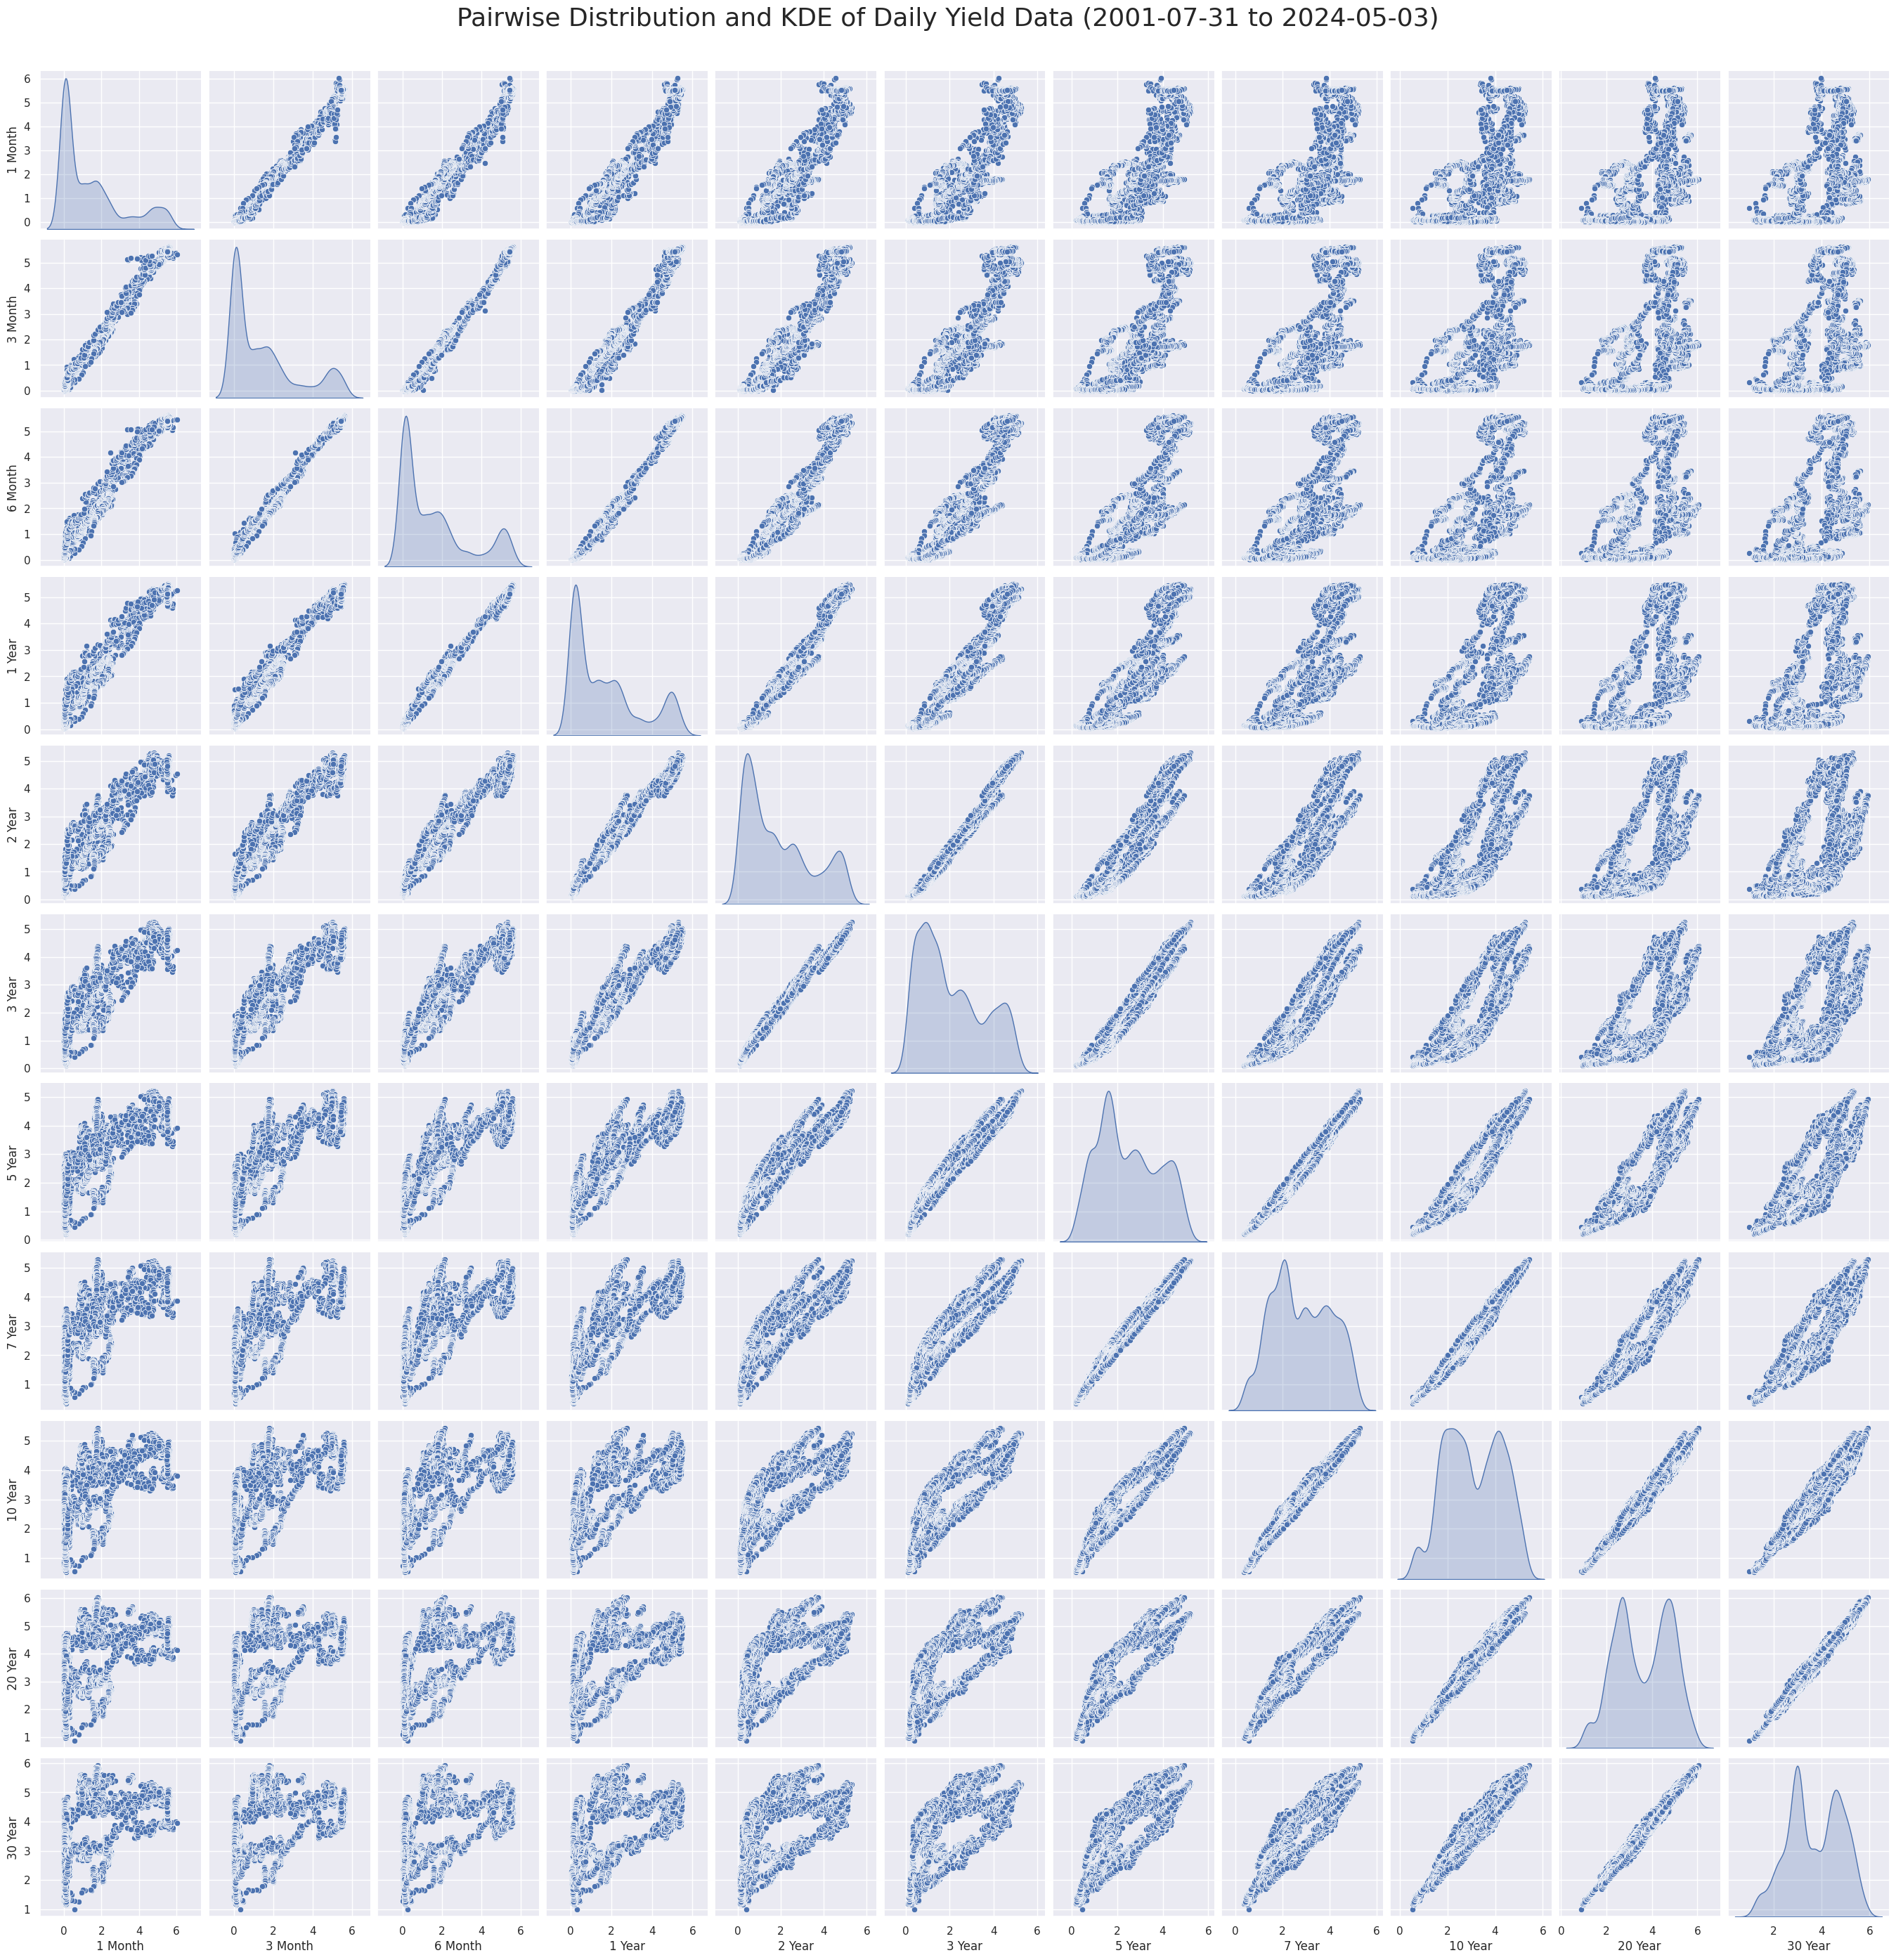
\includegraphics[width=1\textwidth]{gfx/m1l2_notes_fig2_pairplot.png}
    \caption{Phân phối theo cặp và Ước lượng mật độ hạt nhân (KDE) của dữ liệu lợi suất hàng ngày}
    \label{fig:m1l2_notes_fig2_pairplot}
\end{figure}

Biểu đồ cặp (pairplot) ở trên hiển thị mối quan hệ giữa Trái phiếu Kho bạc Hoa Kỳ ở các kỳ hạn khác nhau. Trên đường chéo, chúng ta có thể thấy ước lượng mật độ hạt nhân (kernel density estimation - KDE) của từng mức lợi suất trong khi các biểu đồ nằm ngoài đường chéo hiển thị các biểu đồ phân tán (scatterplots) cho mỗi cặp.

Điều đầu tiên chúng ta nhận thấy là KDE của các mức lợi suất có dạng đa đỉnh (multimodal). Điều này phản ánh tác động của các chế độ kinh tế, chu kỳ, thay đổi chính sách và các sự kiện quan trọng khác nhau lên lợi suất.

Thêm vào đó, các biểu đồ phân tán cho thấy mối tương quan dương mạnh mẽ giữa các mức lợi suất. Cụ thể hơn, các lợi suất có kỳ hạn gần nhau có mối tương quan hoàn hảo (gần bằng 1) trong khi các lợi suất xa nhau vẫn có tương quan dương mặc dù không hoàn hảo.

Hãy trực quan hóa các lợi suất tại một ngày cụ thể:

\begin{lstlisting}[language=Python]
In [8]: # Figure 3
        def plot_yield_curve(date):
            maturities = ['1M', '3M', '6M', '1Y', '2Y', '3Y', '5Y', '7Y', '10Y', '20
            fig, ax = plt.subplots(figsize=(12, 6))
            ax.plot(maturities, yields.loc[date], marker='D', label='Yield Curve at 
            
            ax.set_yticklabels(['{:.2f}%'.format(y) for y in ax.get_yticks()])
            ax.set_xticks(range(len(maturities)))
            ax.set_xticklabels(maturities)
            
            # Add labels and title
            ax.set_xlabel('Maturity')
            ax.set_ylabel('Yield')
            ax.set_title('Treasury Yield Curve')
            
            fig.legend(loc = [0.69, 0.14])
            
            # Show the plot
            plt.grid(True)
            plt.show()

        plot_yield_curve('2020-01-03')
\end{lstlisting}

\begin{lstlisting}[language=Python]
/tmp/ipykernel_17/2521112310.py:8: UserWarning: set_ticklabels() should only 
be used with a fixed number of ticks, i.e. after set_ticks() or using a Fixe
dLocator.
  ax.set_yticklabels(['{:.2f}%'.format(y) for y in ax.get_yticks()])
\end{lstlisting}

\begin{figure}[htbp]
    \centering
    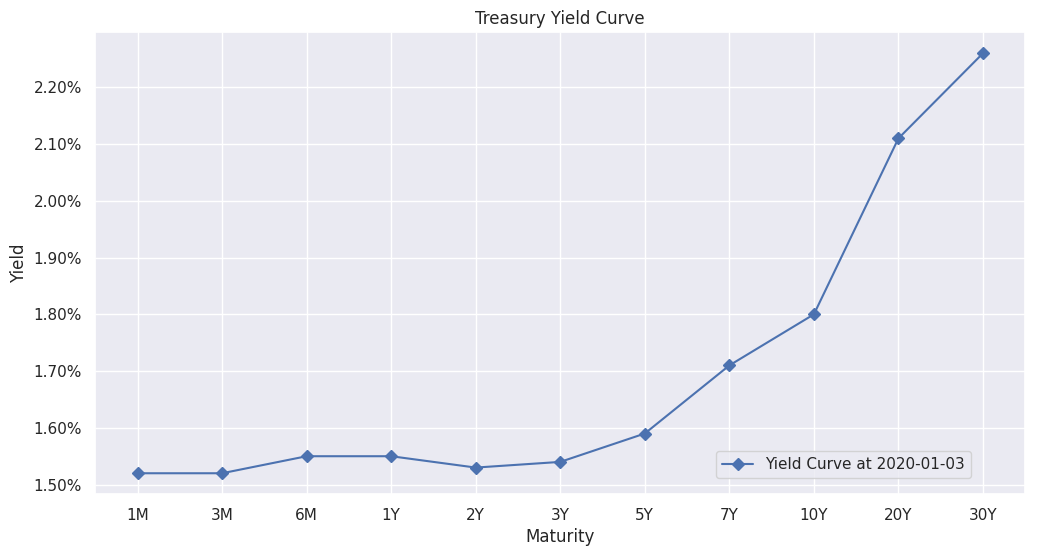
\includegraphics[width=1\textwidth]{gfx/m1l2_notes_fig3_yield_curve_2020.png}
    \caption{Đường cong lợi suất Trái phiếu Kho bạc ngày 03-01-2020}
    \label{fig:m1l2_notes_fig3_yield_curve_2020}
\end{figure}

Bài tập 2
Biểu đồ trên hiển thị tất cả các lợi suất tại ngày 2020-01-03. Hãy tìm (một hoặc hai) ngày cụ thể giúp bạn vẽ lại biểu đồ trên hai lần: một lần cho một đường cong dẹt (flattened curve) và một lần cho một đường cong đảo ngược (inverted curve). Lập luận xem các đường cong dẹt và đường cong đảo ngược tương ứng với các giai đoạn cụ thể nào của Hình 1 (trong một số trường hợp, các đường lợi suất kết hợp trông rất mỏng). Tại sao những ngày đó lại quan trọng?

\subsection[Hình dạng của Đường cong Lợi suất]{Hình dạng của Đường cong Lợi suất (The Shape of the Yield Curve)}

Bằng cách kiểm tra Hình 3 cùng với các hình ảnh mà bạn đã tạo ra khi trả lời Bài tập 2, bạn đã quan sát thấy rằng các yếu tố (rõ ràng nhất) định hình đường cong lợi suất là (Rebonato):
1. Mức độ (level) tổng thể của đường cong lợi suất, biểu thị mức lãi suất đang cao hay thấp như thế nào.
2. Độ dốc (slope) của đường cong lợi suất, cho biết đường cong dốc, phẳng hay đảo ngược như thế nào.

Thông thường, chúng ta có thể giải thích khoảng 90\% sự biến thiên của đường cong thông qua mức độ và độ dốc (Oprea). Để phân tích kỹ lưỡng hơn, người ta cần tính đến yếu tố thứ 3: Độ cong (curvature), đây là thước đo cách thức phần giữa của đường cong (lãi suất trung hạn) hoạt động so với lãi suất ngắn hạn và dài hạn.

Vì mục đích của bài học này, chúng ta sẽ nhấn mạnh vào hai yếu tố đầu tiên.

\subsubsection[Mức độ của Đường cong]{Mức độ của Đường cong (Level of the Curve)}

Mức độ gắn liền với những dịch chuyển song song trong toàn bộ đường cong lợi suất. Về cơ bản, nó ảnh hưởng đến tất cả giá trái phiếu bất kể kỳ hạn với biên độ (gần như) giống nhau. Những dịch chuyển này được thúc đẩy bởi các yếu tố kinh tế vĩ mô như lạm phát, các sự kiện địa chính trị, thay đổi trong chính sách tiền tệ, v.v.

Chúng ta sẽ xem xét Cuộc khủng hoảng Thị trường Trái phiếu năm 1994, còn được gọi là Cuộc Thảm sát Trái phiếu Vĩ đại (Great Bond Massacre). Tác nhân chính dẫn đến sự sụp đổ của trái phiếu là quyết định của Fed khởi xướng một đợt tăng lãi suất. Vào tháng 2 năm 1994, Fed đã nâng lãi suất quỹ từ 3.00\% lên 3.25\%. Trong suốt cả năm, Fed tiếp tục tăng lãi suất theo từng bước, đạt 5.5\% vào tháng 2 năm 1995. Động lực chính đằng sau quyết định của Fed là kỳ vọng lạm phát do sự mở rộng kinh tế nhanh chóng vào năm 1993.

Hơn nữa, trước năm 1994, mức chênh lệch (spread) giữa lãi suất ngắn hạn và dài hạn là hơn 4 điểm phần trăm, dẫn đến việc nhiều nhà đầu tư ở các vị thế đòn bẩy vay ngắn hạn và đầu tư vào các trái phiếu dài hạn hơn. Đương nhiên, những đợt tăng lãi suất đột ngột đã khiến những nhà đầu tư này (trong số những người khác) mất cảnh giác, buộc họ phải tháo gỡ vị thế của mình, dẫn đến một đợt bán tháo trên thị trường trái phiếu.

\begin{lstlisting}[language=Python]
In [9]: # Figure 4
        from matplotlib.gridspec import GridSpec
        
        # Preparing the data
        bond_market_crash = yields.loc['1994-01-03':'1994-11-30'].iloc[::] * 100
        resampled_monthly_bond_market_crash = bond_market_crash.resample('M').last()
        resampled_monthly_bond_market_crash_ticks = resampled_monthly_bond_market_cr
        
        # Creating the plt object
        fig = plt.figure(figsize=(16, 12))
        gs = GridSpec(2, 2, height_ratios=[1, 1.5])
        
        # First row, first column
        ax1 = fig.add_subplot(gs[0, 0])
        ax1.plot(bond_market_crash, alpha=0.7)
        ax1.set_title('Treasury Yields across time - Graph 1')
        ax1.set_xlabel('Date')
        ax1.set_ylabel('Yield (%)')
        ax1.tick_params(axis='x', rotation=45)
        
        # First row, second column
        ax2 = fig.add_subplot(gs[0, 1])
        ax2.bar(resampled_monthly_bond_market_crash_ticks, resampled_monthly_bond_ma
        ax2.set_title('Mean Yields across time - Graph 2')
        ax2.set_xlabel('Date')
        ax2.set_ylabel('Average Yield (%)')
        ax2.tick_params(axis='x', rotation=45)
        
        # Second row
        ax3 = fig.add_subplot(gs[1, :])
        for i in range(len(resampled_monthly_bond_market_crash)):
            date = resampled_monthly_bond_market_crash_ticks[i]
            resampled_monthly_bond_market_crash.iloc[i].plot(ax=ax3, alpha=0.7, l
        
        ax3.set_title('Yield Curves at the end of each month - Graph 3')
        ax3.set_xlabel('Maturity')
        ax3.set_ylabel('Yield (%)')
        ax3.legend(title='Date', loc='center left', bbox_to_anchor=(1, 0.5))
        ax3.tick_params(axis='x', rotation=45)
        
        plt.tight_layout()
        plt.show()
\end{lstlisting}

\begin{lstlisting}[language=Python]
/tmp/ipykernel_17/3704098406.py:7: FutureWarning: 'M' is deprecated and will
be removed in a future version, please use 'ME' instead.
  resampled_monthly_bond_market_crash = bond_market_crash.resample('M').last
()
\end{lstlisting}

\begin{figure}[htbp]
    \centering
    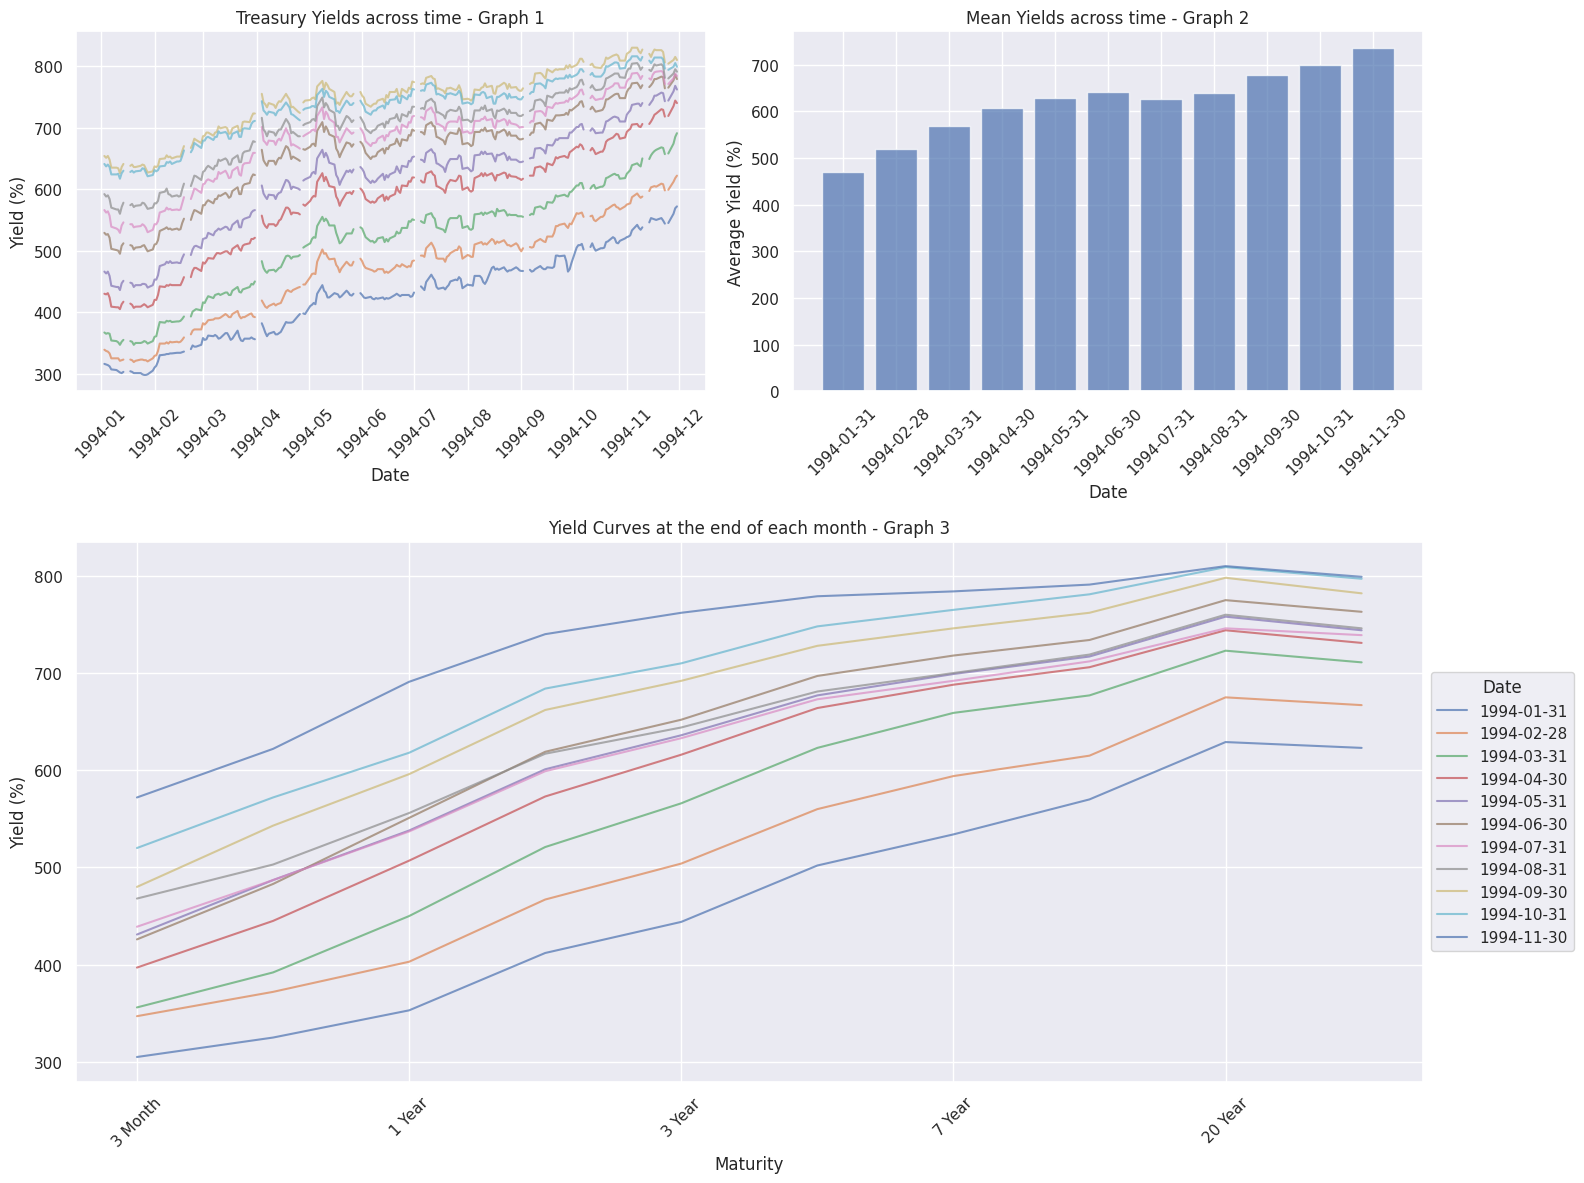
\includegraphics[width=1\textwidth]{gfx/m1l2_notes_fig4_bond_crash_1994.png}
    \caption{Khủng hoảng Thị trường Trái phiếu 1994}
    \label{fig:m1l2_notes_fig4_bond_crash_1994}
\end{figure}

Trong Hình 4, người ta có thể thấy sự dịch chuyển tăng lên nhất quán của lợi suất qua tất cả các kỳ hạn. Cụ thể trong Đồ thị 3, chúng ta quan sát thấy mọi đường cong lợi suất vào cuối mỗi tháng trong năm 1994 (ngày cuối cùng của mỗi tháng được chọn ngẫu nhiên để đại diện cho tháng đó). Đây là một ví dụ điển hình về sự thay đổi mức độ của các lợi suất, nơi toàn bộ đường cong đang di chuyển lên trên mỗi tháng trong khi vẫn giữ nguyên độ dốc của nó.

\subsubsection[Độ dốc của Đường cong Lợi suất]{Độ dốc của Đường cong Lợi suất (Slope of the Yield Curve)}

Độ dốc của đường cong lợi suất thường chỉ sự chênh lệch lợi suất giữa trái phiếu dài hạn và ngắn hạn. Chúng ta thường sử dụng sự chênh lệch giữa trái phiếu 10 năm và 2 năm hoặc giữa trái phiếu 30 năm và 3 tháng, nhưng tùy thuộc vào bối cảnh, người ta có thể chọn các kỳ hạn khác nhau. Độ dốc có thể được phân loại thành:
\begin{enumerate}
    \item Độ dốc dương (positive slope), còn được gọi là đường cong lợi suất bình thường (normal yield curve), xảy ra khi lợi suất dài hạn cao hơn lợi suất ngắn hạn. Đây là kịch bản "bình thường" vì chúng ta kỳ vọng rằng rủi ro bổ sung khi nắm giữ trái phiếu dài hạn sẽ được bù đắp bằng lợi nhuận cao hơn so với trái phiếu ngắn hạn.
    \item Độ dốc phẳng (flat slope): lợi suất ngắn hạn và dài hạn là tương đương nhau.
    \item Độ dốc âm (negative slope), còn được gọi là đường cong lợi suất đảo ngược (inverted yield curve). Nó xảy ra khi lợi suất ngắn hạn cao hơn lợi suất dài hạn.
\end{enumerate}

Như chúng ta đã thấy cho đến hiện tại, độ dốc có thể dễ dàng nhìn thấy trong biểu đồ đường cong lợi suất. Nhưng còn động lực học của những thay đổi độ dốc thì sao?

Giả sử chúng ta đang ở vị trí mà đường cong lợi suất là bình thường. Từ điểm này, độ dốc có thể trở nên dốc hơn (steepen) hoặc phẳng ra (flatten), và trong mỗi trường hợp, điều này có thể xảy ra theo nhiều cách:

\begin{enumerate}
    \item Trở nên dốc hơn (Steepening)
    \begin{itemize}
        \item Đường cong dốc lên do thị trường giá lên (Bull steepening): lãi suất ngắn hạn giảm nhanh hơn lãi suất dài hạn
        \item Đường cong dốc lên do thị trường giá xuống (Bear steepening): lãi suất dài hạn tăng nhanh hơn lãi suất ngắn hạn
    \end{itemize}
    \item Phẳng ra (Flattening)
    \begin{itemize}
        \item Đường cong dẹt đi do thị trường giá lên (Bull flattening): lãi suất dài hạn giảm nhanh hơn lãi suất ngắn hạn
        \item Đường cong dẹt đi do thị trường giá xuống (Bear flattening): lãi suất ngắn hạn tăng nhanh hơn lãi suất dài hạn
    \end{itemize}
\end{enumerate}

Trong Hình 5, bạn có thể thấy một sự thể hiện trực quan về động lực học phẳng ra của đường cong.

\begin{lstlisting}[language=Python]
In [10]: # Figure 5
         # Preparing the data
         bear_flattening = yields['2004-06-01':'2006-06-30'].resample('3M').last()
         bear_flattening.index = bear_flattening.index.strftime('%Y-%m-%d')
         
         bull_flattening = yields['2010-01-01':'2012-06-30'].resample('4M').last()
         bull_flattening.index = bull_flattening.index.strftime('%Y-%m-%d')
         
         # Creating the plt object
         fig, (ax1, ax2) = plt.subplots(1, 2, figsize=(16, 6))
         
         # Bear flattening graph
         for i in range(len(bear_flattening)):
             date = bear_flattening.index[i]
             ax1.plot(bear_flattening.columns, bear_flattening.iloc[i, :], alpha=0.7, 
         
         ax1.set_title('Bear Flattening: 2004 - 2006')
         ax1.set_xlabel('Maturity')
         ax1.set_ylabel('Yield (%)')
         ax1.legend(title='Date', loc='center left', bbox_to_anchor=(1, 0.5))
         ax1.tick_params(axis='x', rotation=45)
         
         # Bull flattening graph
         for i in range(len(bull_flattening)):
             date = bull_flattening.index[i]
             ax2.plot(bull_flattening.columns, bull_flattening.iloc[i, :], alpha=0.7,
         
         ax2.set_title('Bull Flattening: 2010 - 2012')
         ax2.set_xlabel('Maturity')
         ax2.set_ylabel('Yield (%)')
         ax2.legend(title='Date', loc='center left', bbox_to_anchor=(1, 0.5))
         ax2.tick_params(axis='x', rotation=45)
         
         plt.tight_layout()
         plt.show()
\end{lstlisting}

\begin{figure}[htbp]
    \centering
    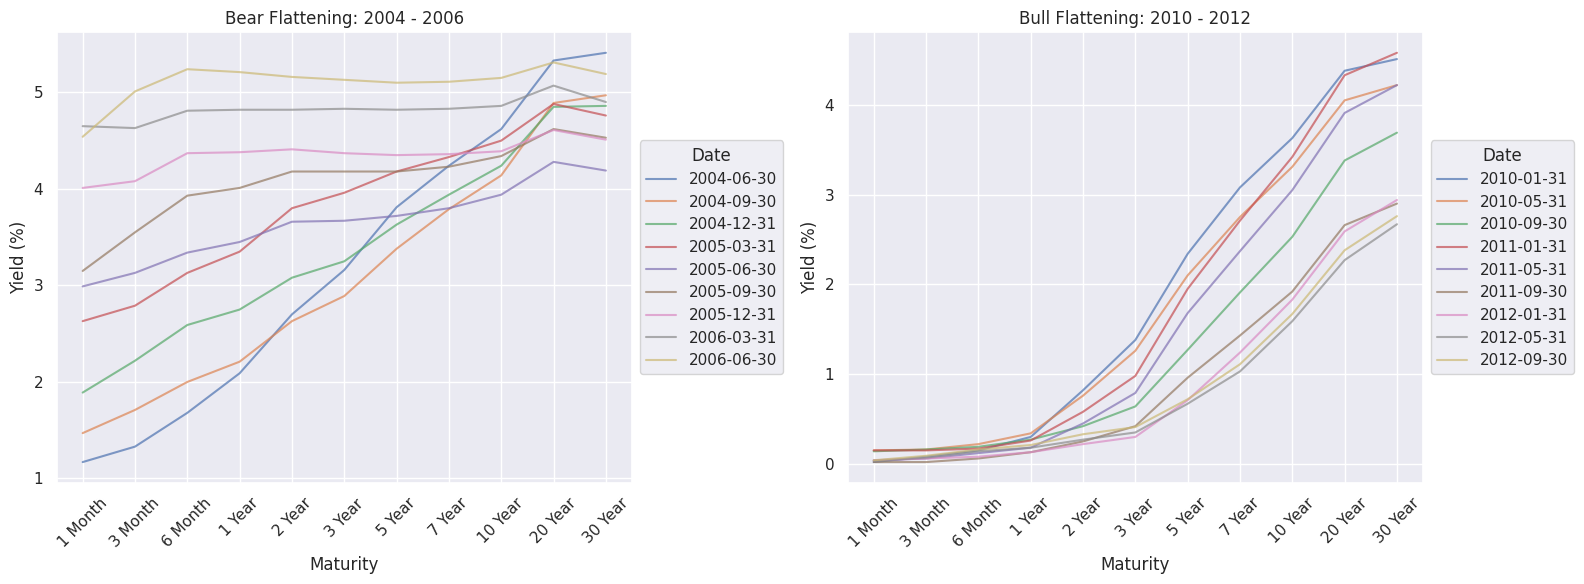
\includegraphics[width=1\textwidth]{gfx/m1l2_notes_fig5_flattening.png}
    \caption{Động lực học phẳng ra của đường cong (Bear Flattening và Bull Flattening)}
    \label{fig:m1l2_notes_fig5_flattening}
\end{figure}

Bài tập 3
Vẽ lại Hình 5 để minh họa các hiện tượng đường cong dốc lên do thị trường giá lên (bull steepening) và giá xuống (bear steepening). Tìm kiếm các khoảng thời gian tương ứng với sự dốc lên của đường cong lợi suất bằng cách tra cứu trực tuyến hoặc trong các sách giáo khoa học thuật, và sử dụng đoạn mã được cung cấp để chứng minh các động lực học của sự dốc lên này. Lập luận về các điều kiện kinh tế và phản ứng của Fed trong những khoảng thời gian này. Dán biểu đồ vào diễn đàn cùng với một đoạn văn nhỏ giải thích những gì chúng ta nhìn thấy.

Bài tập 4
Chứng minh tầm quan trọng của chênh lệch giữa trái phiếu 10 năm và 2 năm. Tạo một biểu đồ có trục y kép (double y-axis plot) trong đó bạn xếp chồng (superimpose) chỉ số S\&P500 lên mức chênh lệch giữa hai trái phiếu này.

\section[Kết luận]{Kết luận (Conclusion)}

Thông qua việc phân tích và trực quan hóa thực hành bằng Python và FRED API, chúng ta đã xem xét động lực học của đường cong lợi suất qua thời gian. Chúng ta đã khám phá cách các yếu tố như mức độ và độ dốc định hình đường cong lợi suất và cách những thành tố này phản ánh cũng như ảnh hưởng đến các điều kiện kinh tế rộng lớn hơn.

Những điểm chính rút ra bao gồm:
\begin{itemize}
    \item Tầm quan trọng của dữ liệu chính phủ mở đối với hoạt động nghiên cứu, hoạch định chính sách và sự hiểu biết của công chúng về các xu hướng kinh tế
    \item Tầm quan trọng của đường cong lợi suất với tư cách là một chỉ báo kinh tế, bao gồm nhiều hình dạng khác nhau của nó (bình thường, phẳng và đảo ngược) và những hình dạng đó có thể biểu thị điều gì về các kỳ vọng kinh tế
    \item Khái niệm đường cong lợi suất dốc lên và dẹt đi cũng như cách những biến động này có thể được phân loại là "bull" (giá lên) hoặc "bear" (giá xuống) tùy thuộc vào những thay đổi lãi suất cơ bản
\end{itemize}

\section*{Tài liệu tham khảo (References)}
\begin{itemize}
    \item Rebonato, Riccardo. Bond Pricing and Yield Curve Modeling: A Structural Approach. Cambridge University Press, 2018.
    \item Oprea, Andreea, The Use of Principal Component Analysis (PCA) in Building Yield Curve Scenarios and Identifying Relative-Value Trading Opportunities on the Romanian Government Bond Market, Journal of Risk and Financial Management, 2022, 15(6), 247
\end{itemize}

Copyright 2024 WorldQuant University. This content is licensed solely for personal use. Redistribution or publication of this material is strictly prohibited.

\chapter{Đọc thêm: Thanh khoản và tác động của cú sốc thông tin (Chương 3)}
\label{ch:M1L2-reading}

\section{Thanh khoản và tác động của các cú sốc thông tin: Ứng dụng trong khóa học Kinh tế Vĩ mô}

Mối quan hệ giữa kinh tế vĩ mô và giá cổ phiếu là cực kỳ quan trọng. Vậy nếu điều đó đúng, thì nền kinh tế ảnh hưởng đến giá cổ phiếu như thế nào và ngược lại? Trong nhiều trường hợp, đó là tin tức về kinh tế vĩ mô và chính xác hơn là tin tức bất ngờ. Việc công bố những tin tức "bất ngờ" về nền kinh tế được gọi là "cú sốc thông tin" (information shocks), thứ có thể có tác động nhanh chóng và đáng kể đến giá cổ phiếu. Các cú sốc thông tin về cơ bản khác với "cú sốc thanh khoản" (liquidity shocks) đã được mô tả trước đó trong chương Tài chính. Trong trường hợp của các cú sốc thanh khoản, chúng ta đã thấy cấu trúc của chính thị trường tài chính cùng với số lượng và chất lượng của các lệnh được gửi có thể ảnh hưởng như thế nào đến khả năng của các nhà đầu tư trong việc tìm ra giá "thực" của một cổ phiếu thông qua quá trình được gọi là "khám phá giá" (price discovery). Trong trường hợp của chúng ta ở đây, các cú sốc thông tin cũng có tác động lớn đến quá trình khám phá giá, nhưng động lực chính của những cú sốc này là sự xuất hiện của những tin tức bất ngờ, chứ không phải do thiếu thanh khoản trong một thị trường tài chính.\footnote{Như đã thảo luận trong chương Tài chính, các thị trường tài chính có thể đạt được "hiệu quả thông tin" nếu chúng xử lý và kết hợp các tin tức bất ngờ một cách nhanh chóng và chính xác vào giá cổ phiếu hiện tại. Theo "giả thuyết thị trường hiệu quả" (EMH), nếu thị trường nhanh chóng và chính xác phản ánh thông tin mới vào giá cổ phiếu, thì hành vi của các mức giá này sẽ giống như một "bước đi ngẫu nhiên" (random walk) và do đó dẫn đến những biến động giá không thể đoán trước theo thời gian. Như đã lưu ý trong chương Tài chính, các thị trường tài chính tương đối hiệu quả nhưng không phải lúc nào cũng hoàn hảo, và do đó có thể mang lại cơ hội cho những nhà đầu tư và nhà giao dịch nhanh nhạy phát hiện ra các xu hướng giá trước khi những người khác khám phá ra.}

Trong chương này, chúng tôi mô tả một số ví dụ về các cú sốc liên quan đến kinh tế vĩ mô và tác động của chúng đối với thị trường chứng khoán Hoa Kỳ, cũng như các mối quan hệ tương hỗ giữa thị trường tài chính và nền kinh tế.

Với quy mô khổng lồ và sự phức tạp của nền kinh tế quốc gia, thông tin liên quan đến kinh tế vĩ mô bao gồm rất nhiều yếu tố. Vậy yếu tố nào là quan trọng nhất? Đầu tiên và quan trọng nhất là lãi suất, thứ áp dụng cho từng công ty cá biệt, các ngành cụ thể, cũng như các lĩnh vực rộng lớn hơn của nền kinh tế. Trong kinh tế vĩ mô, mối quan hệ chủ yếu tập trung vào sự tương tác giữa lãi suất, khu vực tư nhân (bao gồm người tiêu dùng, nhà đầu tư và doanh nghiệp) và các nhà hoạch định chính sách của chính phủ tại Cục Dự trữ Liên bang (thông qua chính sách tiền tệ) và Bộ Tài chính Hoa Kỳ (thông qua chính sách tài khóa). Do lãi suất đại diện cho giá thuê vốn (rental price of money), nên chúng đóng vai trò là cầu nối chính giữa "thế giới thực" của kinh tế vĩ mô và "thế giới tài chính" của thị trường cổ phiếu và trái phiếu. Cả khu vực tư nhân và chính phủ đều theo dõi sát sao lãi suất như một tín hiệu về tình trạng hiện tại và tương lai của nền kinh tế nhằm đưa ra các quyết định phân bổ nguồn lực khan hiếm vào những mục đích sử dụng hiệu quả nhất. Thông qua thanh khoản do thị trường tài chính cung cấp, các nhà đầu tư có thể chuyển các khoản tiết kiệm của mình vào những khoản đầu tư sinh lời, điều này cuối cùng dẫn đến tăng trưởng kinh tế mạnh mẽ hơn cho xã hội. Do đó, các nhà kinh tế học và nhà đầu tư nên xem xét thanh khoản của thị trường tài chính để hiểu rõ hơn về cách thế giới tài chính và thế giới thực tương tác với nhau.

\subsection{Điều kiện kinh tế, Chu kỳ kinh doanh và Vai trò của Lãi suất}

Động lực chính của những biến động chu kỳ kinh doanh ở hầu hết các quốc gia là đầu tư của doanh nghiệp, và những thay đổi đột ngột trong đầu tư này có thể dẫn đến bùng nổ kinh tế cũng như suy thoái. Do đó, các giám đốc điều hành kinh doanh liên tục đánh giá bối cảnh kinh tế để xem người tiêu dùng đang mua gì (và với số lượng bao nhiêu), cũng như theo dõi niềm tin của người tiêu dùng để quyết định mức độ đầu tư cho tương lai. Khi nhu cầu của người tiêu dùng tăng và giảm, các doanh nghiệp phản ứng nhanh chóng bằng cách điều chỉnh số lượng đầu tư vào nhà máy, thiết bị, hàng tồn kho, nghiên cứu và công nghệ mới. Những điều chỉnh này có thể dẫn đến những thay đổi mạnh mẽ về việc làm và tiền lương, từ đó tác động đến những thay đổi tiếp theo trong mô hình chi tiêu của người tiêu dùng. Mối quan hệ giữa đầu tư và tiêu dùng là mang tính tuần hoàn, và điều này dẫn đến tính chất chu kỳ của hầu hết các nền kinh tế, khi các đợt bùng nổ được theo sau bởi các cuộc suy thoái, cuối cùng dẫn đến sự phục hồi và sau đó là các đợt bùng nổ kinh tế tiếp theo.

Lãi suất cũng bị ảnh hưởng lớn bởi đầu tư của doanh nghiệp vì các công ty thường vay tiền từ những người cho vay và các nhà đầu tư để tài trợ cho việc mở rộng trong tương lai. Nhu cầu tiền mặt gia tăng này tạo áp lực làm tăng lãi suất trừ khi ngân hàng trung ương của một quốc gia, chẳng hạn như Cục Dự trữ Liên bang Hoa Kỳ (thường được gọi là "Fed"), tăng cung tiền.

Sự tương tác giữa đầu tư và lãi suất rất phức tạp vì các tác động có thể diễn ra đồng thời về bản chất. Cụ thể, đầu tư kinh doanh không chỉ ảnh hưởng đến lãi suất, mà mức lãi suất, đến lượt nó, lại ảnh hưởng đến mức độ đầu tư. Ví dụ, nếu người tiêu dùng đột nhiên mua nhiều hàng hóa và dịch vụ hơn, các doanh nghiệp sẽ đầu tư nhiều hơn và cuối cùng sẽ đẩy lãi suất lên do nhu cầu tiền mặt tăng. Tuy nhiên, nếu lãi suất tăng quá cao, các doanh nghiệp sẽ cắt giảm đầu tư vì chi phí tài trợ cho nhà máy, thiết bị mới hoặc hàng tồn kho lúc này có thể vượt quá lợi nhuận mà doanh nghiệp có thể kiếm được từ khoản đầu tư mới này. Cuối cùng, việc giảm đầu tư do lãi suất cao hơn sẽ dẫn đến nhu cầu tiền mặt thấp hơn. Điều này sau đó sẽ khiến lãi suất giảm trong tương lai, từ đó tạo ra một chu kỳ kinh điển giữa đầu tư và lãi suất.

Do đó, những thay đổi trong đầu tư kinh doanh được theo dõi sát sao bởi các nhà hoạch định chính sách, chẳng hạn như những người tại Cục Dự trữ Liên bang. Fed sẽ cố gắng kích thích và ổn định nền kinh tế bằng cách điều chỉnh lãi suất Quỹ Liên bang (Federal Funds rate)\footnote{Lãi suất Quỹ Liên bang là mức lãi suất mà các ngân hàng thương mại tính cho nhau khi vay qua đêm để đáp ứng nhu cầu thanh khoản ngắn hạn.} nhằm duy trì sự tăng trưởng ổn định với lạm phát thấp. Để điều chỉnh mức lãi suất chủ chốt này lên (hoặc xuống), Fed thường sử dụng các nghiệp vụ thị trường mở ("OMO") để bán (hoặc mua) chứng khoán Kho bạc Hoa Kỳ (U.S. Treasury securities) trên các thị trường trái phiếu chính phủ, nơi các đối tác giao dịch chính là các tổ chức tài chính như ngân hàng thương mại và các nhà môi giới chứng khoán (broker-dealers). Khi Fed bán Trái phiếu Kho bạc qua các hoạt động OMO, mục tiêu là giảm cung tiền và tăng lãi suất Quỹ Liên bang (giả sử nhu cầu tiền mặt vẫn tương đối ổn định). Bằng cách bán Trái phiếu Kho bạc, Fed đang rút đô la khỏi nền kinh tế và làm giảm cung tiền do các nhà đầu tư phải từ bỏ tiền mặt của họ để mua các chứng khoán chính phủ này. Các nhà kinh tế gọi đây là chính sách tiền tệ "thắt chặt" (contractionary monetary policy) bởi vì mục tiêu của việc tăng mức lãi suất then chốt này là khiến các ngân hàng và những người cho vay khác tăng lãi suất cho vay của họ, và qua đó, làm cho các doanh nghiệp và người tiêu dùng phải chịu chi phí cao hơn để chi trả cho các khoản đầu tư và tiêu dùng bổ sung. Điều này cuối cùng có thể dẫn đến sự thu hẹp của nền kinh tế thông qua việc giảm đầu tư của doanh nghiệp, vì lãi suất cao hơn có thể "làm nguội" một nền kinh tế đang trên đà "quá nóng" do lạm phát giá cả gia tăng. Ngược lại, một chính sách tiền tệ "mở rộng" (expansionary monetary policy) xảy ra khi Fed mua Trái phiếu Kho bạc để bơm thêm tiền vào nền kinh tế nhằm giảm lãi suất Quỹ Liên bang và kích thích đầu tư từ các doanh nghiệp và người tiêu dùng.

\subsection{Cục Dự trữ Liên bang và Mối liên kết giữa Kinh tế vĩ mô và Thị trường Tài chính}

Hoạt động OMO của Fed tạo ra một "vòng phản hồi tương tác" (interactive feedback loop) liên tục giữa nền kinh tế vĩ mô và thị trường tài chính. Khi các điều kiện kinh tế vĩ mô và lãi suất thay đổi, cả Fed và các thành viên tham gia thị trường như ngân hàng, nhà môi giới và nhà quản lý tài sản đều điều chỉnh danh mục nắm giữ của họ, không chỉ đối với chứng khoán Kho bạc Hoa Kỳ mà còn đối với các tài sản rủi ro hơn như trái phiếu doanh nghiệp và cổ phiếu vốn cổ phần. Các nhà đầu tư trên thị trường tài chính phản ứng với những tin tức bất ngờ về nền kinh tế và lãi suất vì giá trị của một cổ phiếu hay trái phiếu được xác định bởi giá trị hiện tại của các dòng tiền mặt dự kiến trong tương lai của nó. Như đã lưu ý trong chương Vi mô, phản ứng này của nhà đầu tư bị thúc đẩy bởi những thay đổi trong lãi suất phi rủi ro, điều này có thể ảnh hưởng đến Đường Thị trường Vốn (Capital Market Line) theo Mô hình Định giá Tài sản Vốn (CAPM). Trong mô hình đó, khi lãi suất phi rủi ro tăng lên, điểm giao cắt (intercept) tăng lên, độ dốc (slope) giảm xuống và điểm tiếp tuyến (tangency) với đường biên hiệu quả (efficient frontier) di chuyển lên trên và sang phải, qua đó làm tăng tỷ suất sinh lợi yêu cầu của các nhà đầu tư đối với danh mục thị trường. Khái niệm Đường Thị trường Vốn giúp giải thích cách thức các hành động và tuyên bố chính sách của Fed có thể tạo ra các cú sốc thông tin, dẫn đến lượng lớn hoạt động giao dịch trong tất cả các loại chứng khoán, điều này ngược lại, phụ thuộc vào thanh khoản của các thị trường tài chính. Thông qua việc giao dịch hàng nghìn tỷ đô la chứng khoán hằng ngày này, các thị trường tài chính phục vụ một mục đích quan trọng là cơ chế chính để khám phá ra mức giá phù hợp cho các tài sản tài chính. Như đã lưu ý trước đó trong các chương Tài chính và Vi mô, khám phá giá là một chức năng chính của bất kỳ thị trường tài chính hoạt động trơn tru nào.

Một ví dụ điển hình về vòng phản hồi tương tác này có thể thấy trong thông báo tháng 10 năm 2018 của Fed về kế hoạch tiếp tục tăng lãi suất và cách chính sách thắt chặt này đã gây sốc cho các thị trường chứng khoán Hoa Kỳ, khiến giá giảm mạnh vào cuối tháng 12 năm 2018. Để phản ứng với phản ứng tiêu cực này của thị trường, chủ tịch Fed, Jerome Powell, đã tuyên bố vào đầu tháng 1 năm 2019 rằng quan điểm thắt chặt của Fed sẽ được "tạm dừng". Các thị trường tài chính coi đây là tin tốt vì lo ngại rằng việc tiếp tục tăng lãi suất Quỹ Liên bang có thể khiến nền kinh tế Hoa Kỳ rơi vào suy thoái. Thị trường chứng khoán Hoa Kỳ đã phản ứng rất tích cực với sự thay đổi trong chính sách tiền tệ này trong quý đầu tiên của năm 2019. Thấy được điều này, Fed cuối cùng đã quyết định cắt giảm lãi suất ba lần, dẫn đến sự gia tăng 29\% của chỉ số S\&P 500 trong năm 2019. Thêm chi tiết về ví dụ này về sự tương tác giữa nền kinh tế và thị trường tài chính sẽ được thảo luận ở phần sau của chương này.

\subsection{Tác động của Cú sốc Thông tin đối với Kỳ vọng Phân kỳ và Khám phá Giá}

Những thay đổi trong chính sách của Fed có thể ảnh hưởng đến thanh khoản của thị trường tài chính không chỉ trực tiếp bằng hoạt động OMO của Fed mà còn thông qua các "tín hiệu" thông tin ẩn chứa trong những thay đổi chính sách này. Ví dụ, một đợt cắt giảm bất ngờ lãi suất Quỹ Liên bang là một cú sốc thông tin có thể ra tín hiệu cho các nhà đầu tư và giám đốc điều hành doanh nghiệp rằng nền kinh tế hiện đang yếu, nhưng đồng thời, nó cũng cho mọi người biết rằng Fed đang hành động để kích thích các điều kiện kinh tế và do đó sẽ củng cố kinh tế vĩ mô trong tương lai. Điều này có thể tạo ra "kỳ vọng phân kỳ" (divergent expectations - một khái niệm được thảo luận trong chương Tài chính), nơi một số thành viên tương đối bi quan của thị trường sẽ giao dịch dựa trên sự suy yếu kinh tế ngắn hạn (ví dụ: bằng cách mua trái phiếu khiến giá trị của chúng tăng lên và lãi suất giảm, đồng thời cũng bán cổ phiếu). Ngược lại, các thành viên lạc quan hơn sẽ tập trung vào những triển vọng tích cực của một nền kinh tế vững mạnh trong dài hạn hơn và chọn đầu tư vào các tài sản rủi ro có khả năng sinh lời tốt trong một nền kinh tế mở rộng (ví dụ: bằng cách bán trái phiếu và mua cổ phiếu).

Trong thuật ngữ của thị trường tài chính, các nhà giao dịch bi quan thường được gọi là "những con gấu" (bears), trong khi các nhà giao dịch lạc quan được miêu tả là "những con bò tót" (bulls). Giao dịch trên các thị trường tài chính giữa hai loại nhà đầu tư này sau đó sẽ giúp khám phá ra mức giá "cân bằng" (equilibrium) thích hợp của cổ phiếu và trái phiếu. Các mức giá này là những tín hiệu mang tính thông tin. Tuy nhiên, không chỉ mất cả một ngày giao dịch mà còn có thể mất vài ngày (hoặc thậm chí vài tuần) để những con bò tót và những con gấu giao dịch với nhau cho đến khi một mức giá cân bằng mới được khám phá. Quá trình khám phá giá kéo dài này xảy ra vì các báo cáo kinh tế được công bố sau cú sốc thông tin ban đầu đôi khi có thể mâu thuẫn về bản chất. Ví dụ, dữ liệu kinh tế theo chiều hướng giá lên (bullish) được công bố vào một ngày có thể được theo sau bởi dữ liệu giá xuống (bearish) vào ngày hôm sau, do đó gieo rắc sự nhầm lẫn về tác động thực sự của các báo cáo này đối với giá của một cổ phiếu.

Để minh họa cho vai trò quan trọng của việc khám phá giá, chúng ta có thể sử dụng một ví dụ được đơn giản hóa dựa trên giá cổ phiếu của một công ty giả định, ABC. Các nghiên cứu học thuật trước đây của Handa, Schwartz và Tiwari (2003) gợi ý rằng chúng ta có thể mô tả sự phân kỳ trong kỳ vọng của các nhà đầu tư bằng cách chia một nhóm người tham gia thành hai nhóm. Hãy gọi một nhóm là "bò tót" và nhóm kia là "gấu". Chúng ta có thể giả định rằng phe bò định giá cổ phiếu ABC ở mức 30 đô la và phe gấu định giá cổ phiếu ABC ở mức 20 đô la. Phe bò là những người mua, và phe gấu là những người bán do sự phân kỳ kỳ vọng về giá trị tương lai của cổ phiếu dựa trên một số tin tức kinh tế vĩ mô bất ngờ như sự thay đổi đột ngột trong chính sách tiền tệ của Cục Dự trữ Liên bang. Giả sử những người tham gia lần lượt đến thị trường tài chính và (1) đăng các lệnh mua hoặc bán hoặc (2) giao dịch ngay lập tức ở mức giá mua hoặc giá chào bán được thiết lập bởi các lệnh đã được đặt trước đó. 

Giá mua và giá chào bán cân bằng cho cổ phiếu ABC có thể được xác định nếu biết thêm một thông tin nữa - tỷ lệ phần trăm những người tham gia là phe bò (ký hiệu là k) và tỷ lệ phần trăm những người tham gia là phe gấu (ký hiệu là $1-k$). Trong bối cảnh được đơn giản hóa này, sự phân kỳ trong kỳ vọng giữa các bên tham gia có hai chiều hướng: (1) độ lớn của chênh lệch giữa các mức định giá cao và thấp (trong trường hợp của chúng ta là $\$30-\$20$) và (2) sự phân bổ của các nhà đầu tư giữa hai định giá (như được thể hiện bởi k). Do đó, giá trị của cổ phiếu ABC sẽ nằm đâu đó trong khoảng từ 20 đô la đến 30 đô la tùy thuộc vào giá trị của k. Ví dụ, nếu một nửa số nhà giao dịch là theo chiều hướng giá lên ($k=.50$), thì giá cân bằng sẽ là 25 đô la (tức là $.50\times\$30$ cộng với $.50\times\$20=\$25$).

Làm thế nào những người tham gia biết hoặc tìm ra giá trị của k? Cách chính là quan sát các lệnh được gửi đến thị trường tài chính. Những lệnh này được tạo ra để phản ứng với tin tức về triển vọng của ABC cũng như các điều kiện kinh tế vĩ mô nói chung. Vì vậy, những người tham gia khám phá ra giá trị của k thông qua các lệnh được tiết lộ trong quá trình giao dịch diễn ra. Khi các giao dịch này được báo cáo cho mọi người nhìn thấy, giá cổ phiếu ABC sẽ biến động để phản ứng với những niềm tin thay đổi về k.

Trong các thị trường thực tế, kỳ vọng phân kỳ của người tham gia được phân bổ trên một phạm vi định giá rộng hơn, và chúng ta không thể chỉ tham chiếu đến một biến k. Tuy nhiên, kết luận vẫn đúng - khi kỳ vọng có sự phân kỳ, giá phải được khám phá thông qua quá trình giao dịch trên các thị trường tài chính. Quá trình này không hề đơn giản và đôi khi có thể lộn xộn, kéo dài khi các nhà đầu tư phải sàng lọc vô số tín hiệu từ cả thị trường tài chính và kinh tế vĩ mô, nhiều trong số đó có thể mâu thuẫn nhau.

\subsection{Các Loại Hình Thị trường Tài chính Khác nhau}

Như đã thảo luận trong ví dụ về sổ lệnh giới hạn của chương Tài chính, một thị trường tài chính mỏng (thin), thanh khoản kém sẽ áp đặt chi phí giao dịch cao hơn cho các nhà đầu tư và có thể ngăn cản một số người tham gia đặt lệnh ngay từ đầu. Ví dụ, trong một thị trường dựa trên sổ lệnh giới hạn (limit order book) thanh khoản kém (còn được gọi là thị trường "điều khiển bằng lệnh" (order-driven) liên tục), một cú sốc thông tin có thể gây ra sự gia tăng đột ngột các lệnh mua hoặc bán, và điều này có thể dẫn đến mức chênh lệch giá chào mua-chào bán (bid-ask spread) rộng hơn. Nếu không có các mức giá chào mua và chào bán mới được đưa vào sổ lệnh giới hạn, mức chênh lệch bid-ask mà các nhà đầu tư phải trả sẽ cao hơn rất nhiều, và do đó, việc giao dịch cổ phiếu của công ty sẽ trở nên đắt đỏ hơn. Ngoài ra, mức chênh lệch cao hơn này có thể dẫn đến sự biến động giá lớn hơn, bởi vì ngay cả khi báo giá mua và báo giá bán tốt nhất vẫn không đổi, giá giao dịch sẽ bật lên bật xuống giữa mức giá chào mua và mức giá chào bán do sự xuất hiện gián đoạn của các lệnh thị trường (market orders) muốn bán khớp với mức giá chào mua thấp hơn, và các lệnh thị trường muốn mua khớp với mức giá chào bán cao hơn nhiều. Tác động này thường được gọi là "bid-ask bounce" (sự nảy lên nảy xuống giữa giá mua và giá bán), và sự nảy này góp phần tạo ra biến động giá trong ngắn hạn.

Giá cổ phiếu cũng trở nên biến động hơn trong một sổ lệnh mỏng (thin order book) do "tác động thị trường" (market impact), xảy ra khi một lệnh mua lớn đẩy giá khớp lệnh lên cao hơn mức giá chào bán tốt nhất, hoặc một lệnh bán lớn đẩy giá xuống thấp hơn mức giá chào mua tốt nhất. Khi tác động thị trường lớn, sự biến động giá sẽ tăng lên do giá thường sẽ quay trở lại (revert) các mức quan sát được ngay trước khi lệnh thị trường lớn đó được đặt. Quá trình khám phá giá cũng có thể trở nên khó khăn hơn trong một thị trường mỏng, và nếu đúng như vậy, điều này cũng sẽ góp phần làm tăng biến động giá.

Hệ quả là, một sổ lệnh mỏng có thể làm cho quá trình khám phá giá khó khăn hơn, từ đó dẫn đến những tín hiệu kém tính thông tin hơn về cách các nhà đầu tư đang phản ứng với những tin tức liên quan đến kinh tế vĩ mô và sức khỏe tài chính của một cổ phiếu cụ thể như ABC. Do đó, các tín hiệu từ một thị trường tài chính kém thanh khoản sẽ "nhiễu" (noisier) hơn so với những tín hiệu được tạo ra bởi một thị trường sâu (deep), có tính thanh khoản cao. Trong trường hợp cực đoan, một thị trường tài chính rất kém thanh khoản bị giáng đòn bởi các cú sốc thông tin thường xuyên sẽ dẫn đến những tín hiệu không đáng tin cậy từ các nhà đầu tư, và vòng phản hồi tương tác giữa kinh tế vĩ mô và thị trường tài chính sẽ bị phá vỡ. Kết quả này là tiêu cực đối với tất cả các bên vì các nhà đầu tư, giám đốc điều hành doanh nghiệp và các nhà hoạch định chính sách không còn có được dòng thông tin tự do luân chuyển về cách hành động của họ đang ảnh hưởng đến cả nền kinh tế vĩ mô và thị trường tài chính. Kết quả là, thanh khoản kém có thể cản trở tăng trưởng kinh tế và làm xói mòn lợi nhuận do cổ phiếu và trái phiếu mang lại.

Bên cạnh cấu trúc sổ lệnh giới hạn, hay cấu trúc thị trường điều khiển bằng lệnh liên tục được mô tả trong chương Tài chính, có hai cách chính khác để tổ chức một thị trường tài chính: (1) đấu giá định kỳ (periodic call auction) và (2) thị trường có sự tham gia của nhà tạo lập thị trường (dealer market - hay còn gọi là thị trường "điều khiển bằng báo giá" (quote-driven)). Phiên đấu giá định kỳ là một thị trường điều khiển bằng lệnh định kỳ (ngược lại với liên tục). Các cấu trúc thị trường thay thế này có thể giúp ích cho những người mua và người bán lớn, những người mà nếu không có các cấu trúc này, có thể sẽ ngần ngại khi đưa lệnh của họ vào một thị trường liên tục điều khiển bằng báo giá. Những nhà giao dịch này e ngại việc nộp các lệnh lớn vì sợ đẩy giá lên hoặc xuống một cách không chính đáng (được gọi là tác động thị trường). Một mối quan ngại khác đối với những người mua/người bán lớn này là việc các nhà giao dịch khác có thể phát hiện ra lệnh của họ, điều này có thể dẫn đến việc giao dịch ở mức giá không thuận lợi (thường được gọi là "rò rỉ thông tin" (information leakage)). Các lệnh không được tiết lộ được gọi là "thanh khoản ngầm" (latent liquidity).

Như đã thảo luận trong chương Tài chính, trong một phiên đấu giá định kỳ (call auction), các lệnh của người tham gia được gom lại cùng nhau để thực hiện đồng thời tại một mức giá thanh toán (clearing price) duy nhất vào một thời điểm đã được thông báo trước. Khi thị trường được gọi (called), tất cả các lệnh mua bằng hoặc lớn hơn mức giá thanh toán đều có thể được thực thi, tương tự như tất cả các lệnh bán bằng hoặc thấp hơn mức giá thanh toán. Các mức giá giao dịch được thiết lập ở những giá trị tối đa hóa số lượng cổ phiếu được khớp lệnh. Bằng cách gom (batching) nhiều giao dịch lại cùng nhau, một phiên đấu giá định kỳ sẽ tập trung được thanh khoản và qua đó, có thể làm giảm đáng kể chi phí giao dịch cho người tham gia. Các phiên đấu giá này cũng tạo điều kiện thuận lợi cho quá trình "khám phá số lượng" (quantity discovery) bằng cách cho phép các lệnh lớn hơn được thực thi với ít tác động thị trường hơn và giảm thiểu sự rò rỉ thông tin. Sự tích hợp giữa thanh khoản được tiết lộ (revealed) và thanh khoản ngầm (latent) có thể được hài hòa tốt hơn trong một phiên đấu giá định kỳ, do người cung cấp thanh khoản ngầm sẽ cảm thấy thoải mái hơn khi tiết lộ các lệnh. Tại sao? Một lý do là: họ có thể nhận được sự cải thiện về giá (price improvement), trong khi, với những ngoại lệ hiếm hoi, điều này không xảy ra với giao dịch theo cơ chế điều khiển bằng lệnh liên tục.

Ngược lại với phiên đấu giá định kỳ, trong thị trường có nhà tạo lập (dealer market), các nhà tạo lập (hay còn gọi là "nhà tạo lập thị trường" - market makers) sẽ đưa ra mức giá mà khách hàng đại chúng có thể mua hoặc bán cổ phiếu. Một nhà tạo lập sẽ đăng báo giá hai chiều: báo giá chào mua (bid quote) là mức giá nhà tạo lập thị trường sẽ mua cổ phiếu nếu khách hàng muốn bán, và báo giá chào bán (ask quote) là mức giá nhà tạo lập thị trường sẽ bán cổ phiếu nếu khách hàng muốn mua. Như đã lưu ý trước đó, thị trường có nhà tạo lập thường được gọi là thị trường điều khiển bằng báo giá. Lợi ích chính của thị trường nhà tạo lập là nó có thể cung cấp tính tức thời (immediacy) bằng cách cho phép người mua và người bán đại chúng tương tác trực tiếp và nhanh chóng với một nhà tạo lập, qua đó những khách hàng này gặp ít rủi ro không được khớp lệnh hơn (được gọi là "rủi ro thực thi" - execution risk). Vì vậy, thị trường nhà tạo lập có thể giảm rủi ro thực thi, nhưng điều này thường đi kèm với sự đánh đổi về mức chênh lệch bid-ask rộng hơn và sự thiếu minh bạch hơn về những người mua và người bán khác trên thị trường.

Ngoài các thị trường điều khiển bằng lệnh liên tục, thị trường điều khiển bằng báo giá và các phiên đấu giá định kỳ, còn có các cơ chế khác để đáp ứng những nhu cầu giao dịch mang tính đặc thù hơn. Ví dụ, cơ chế giao dịch khối (block trading) được sử dụng để xử lý các lệnh quy mô lớn của các nhà đầu tư lớn (thường là các tổ chức) đang cố gắng hạn chế tác động bất lợi từ các lệnh lớn của họ đối với các mức giá mà cuối cùng họ sẽ giao dịch. Một lệnh lớn, thường được định nghĩa là lệnh mua từ 10.000 cổ phiếu trở lên, có thể được thương lượng trực tiếp giữa người với người (mặt đối mặt, qua điện thoại hoặc tin nhắn tức thời) hoặc được thực hiện qua giao diện điện tử.

Khi công nghệ mới xuất hiện, thị trường tài chính và các chiến lược giao dịch của nhà đầu tư không ngừng phát triển. Ví dụ, các cơ chế giao dịch tương đối mới cho phép các lệnh được giao dịch mà không cần tiết lộ công khai lợi ích giao dịch của họ được gọi là "dark pools" (hồ tối). Dark pools là các diễn đàn giao dịch tư nhân, đối lập với giao dịch diễn ra trên các sàn giao dịch công cộng như Sàn Giao dịch Chứng khoán New York (New York Stock Exchange) và Nasdaq. Những cơ chế này được đặt tên như vậy nhằm nhấn mạnh sự thiếu minh bạch của chúng so với các sàn giao dịch công cộng "sáng" (lit). Dù dark pools ban đầu ra đời chủ yếu để hỗ trợ giao dịch khối lượng lớn của các nhà đầu tư tổ chức, nhưng hiện tại chúng được sử dụng để giao dịch cho cả những lệnh quy mô nhỏ và lớn. Những lệnh bán lẻ nhỏ do các công ty môi giới lớn nhận được có thể được thực hiện nội bộ, không cần gửi đến các sàn giao dịch công cộng, và đây cũng được coi là một hình thức giao dịch dark pool.

Dark pools được gọi là "dark" (tối) để phân biệt chúng với các thị trường "lit" (sáng). Các sàn giao dịch chứng khoán công cộng được coi là "sáng" nhờ mức độ minh bạch cao hơn của sổ lệnh. Các quy tắc sau được áp dụng: (1) quá trình khám phá giá thường diễn ra thông qua giao dịch trên các sàn giao dịch công cộng; (2) các mức giá này sau đó được sử dụng cho giao dịch trong các dark pools; và (3) dark pools tăng cường khả năng khám phá số lượng, đặc biệt là đối với những người tham gia lớn, những người mà nếu không có dark pool, sẽ e ngại việc gửi lệnh của họ đến các thị trường sáng. Sự chia tách ngày càng tăng giữa khám phá giá và khám phá số lượng không phải là không có những mặt hạn chế. Các giá trị hiệu quả cho cả giá và số lượng sẽ đạt được tốt hơn khi cả hai biến số được xác định đồng thời. Thú vị là, hai yếu tố này được xác định đồng thời trong giao dịch thông qua đấu giá định kỳ (call auction).

Với các mô hình cấu trúc thị trường cạnh tranh được mô tả ở trên, bạn có thể thắc mắc: đâu là mô hình tốt nhất để sử dụng cho giao dịch? Như trong nhiều trường hợp, câu trả lời là "còn tùy" vào nhu cầu của khách hàng. Do các loại nhà giao dịch khác nhau (ví dụ: cá nhân so với tổ chức) có các nhu cầu khác nhau, không có gì ngạc nhiên khi các sàn giao dịch và các địa điểm giao dịch khác hiện cung cấp nhiều mô hình cấu trúc thị trường dưới dạng "lai" (hybrid). Ví dụ, các sàn giao dịch chứng khoán quốc tế lớn thường mở cửa và đóng cửa giao dịch bằng một phiên đấu giá định kỳ, và một số nơi có các phiên đấu giá giữa ngày. Việc gom các lệnh trong một hệ thống giao dịch đấu giá định kỳ đa phương giúp tạo thuận lợi cho việc xử lý lệnh, mài giũa quá trình khám phá giá và nâng cao tính minh bạch của thị trường. Các phiên đấu giá định kỳ không cung cấp tính tức thời, nhưng giao dịch trên thị trường liên tục thì có. Tính tức thời được cung cấp bởi một thị trường liên tục theo ngay sau một phiên đấu giá mở cửa có sức hấp dẫn vô cùng lớn đối với những người tham gia thị trường. Vì vậy, một cấu trúc thị trường lai kết hợp giữa giao dịch liên tục và đấu giá định kỳ mang lại những lợi thế đáng kể. Hơn nữa, khi chịu áp lực nghiêm trọng, quá trình khám phá giá trong thị trường liên tục bị sụp đổ, giao dịch bị tạm dừng và thị trường được mở cửa lại bằng một phiên đấu giá định kỳ.

Bất kể cấu trúc cụ thể của thị trường tài chính là gì, Fed và các quan sát viên kinh tế khác đều cần chú ý đến thanh khoản của những thị trường này. Các nhà đầu tư tại các địa điểm giao dịch này không chỉ phản ứng với tín hiệu từ Fed mà còn tự tạo ra các tín hiệu về quan điểm của họ đối với kinh tế vĩ mô thông qua các mô hình giao dịch của họ. Do đó, những biến động giá trên thị trường trái phiếu và cổ phiếu được Fed và Bộ Tài chính Hoa Kỳ sử dụng để xem liệu các hành động mở rộng và thắt chặt của họ có đang mang lại hiệu ứng phù hợp đối với nền kinh tế hay không, cũng như để đánh giá phản ứng của nhà đầu tư đối với các chính sách mà họ công bố. Mối quan hệ đồng thời giữa hành động của nhà đầu tư, giám đốc doanh nghiệp và nhà hoạch định chính sách tạo ra một hệ thống liên kết chặt chẽ, có khả năng phân bổ nguồn lực kinh tế khan hiếm một cách hiệu quả hơn nhằm kiến tạo một nền kinh tế vĩ mô vận hành trơn tru và năng suất. Như đã lưu ý trước đó, mối liên kết này giữa "thế giới thực" và "thế giới tài chính" phụ thuộc rất lớn vào thanh khoản của các thị trường tài chính, được cung cấp bởi các cấu trúc thị trường đa dạng mà chúng tôi vừa trình bày.

\subsection{Ví dụ về một Cú sốc Thông tin Dựa trên các Hành động của Fed và Phản ứng của Thị trường Tài chính}

Để minh họa cho một số cú sốc thông tin liên quan đến kinh tế và sự tương tác giữa nền kinh tế với thị trường tài chính, chúng ta có thể kiểm tra cách các phát biểu của Chủ tịch Fed Jerome Powell vào đầu tháng 10 năm 2018 về khả năng tiếp tục tăng lãi suất Quỹ Liên bang đã gây ra sự sụt giảm mạnh mẽ trên thị trường chứng khoán trong quý IV năm 2018. Chỉ số thị trường chứng khoán S\&P 500 đã giảm 14,0\% từ cuối tháng 9 năm 2019 đến cuối tháng 12 năm 2019. Phản ứng tiêu cực nhanh chóng và mạnh mẽ của thị trường chứng khoán và trái phiếu đối với tuyên bố bất ngờ của Powell rằng "còn một chặng đường dài" trước khi các đợt tăng lãi suất tiếp theo dừng lại, đã thúc đẩy chủ tịch Fed tuyên bố vào đầu tháng 1 năm 2019 rằng Fed thay vào đó sẽ thể hiện "sự kiên nhẫn" trong việc tăng lãi suất thêm. Thị trường chứng khoán ngay lập tức phục hồi tăng +3,4\% vào đúng ngày Powell bình luận về cách tiếp cận chậm hơn đối với việc tăng lãi suất Quỹ Liên bang. Fed đã giữ nguyên lãi suất trong phần lớn năm 2019 và sau đó thực sự bắt đầu hạ lãi suất từ tháng 8 đến tháng 11 năm 2019. Ba đợt cắt giảm liên tiếp 0,25\% đối với lãi suất Quỹ Liên bang đã kéo nó từ mức 2,0-2,5\% vào mùa hè 2019 xuống còn 1,50-1,75\% vào tháng 11 năm 2019. Fed gọi sự thay đổi từ chính sách tiền tệ thắt chặt sang mở rộng này là một "sự điều chỉnh giữa chu kỳ" (mid-cycle adjustment) do có những lo ngại về nguy cơ nền kinh tế tăng trưởng chậm lại. Các tuyên bố của Fed trong tháng 1, tiếp nối bằng các đợt cắt giảm lãi suất vào cuối năm đó, đã góp phần thúc đẩy sự phục hồi nhanh chóng và mạnh mẽ của cổ phiếu trong năm 2019, với chỉ số chứng khoán S\&P 500 tăng 29\% trong suốt cả năm, từ mức 2.506,85 lên 3.230,78.

Chuỗi sự kiện được mô tả ở trên đại diện cho một ví dụ rõ ràng về vòng phản hồi liên tục giữa kinh tế vĩ mô và thị trường tài chính. Dưới đây chúng tôi trình bày một số biểu đồ và mục tin tức liên quan đến các sự kiện đã diễn ra từ tháng 10 năm 2018 đến tháng 12 năm 2019.

Tin tức bất ngờ được tiết lộ đầu tiên thông qua tuyên bố của Chủ tịch Fed Powell vào đầu tháng 10 năm 2018 đã được CNBC.com trích dẫn như sau: "Chúng tôi [tức là Fed] có thể sẽ tiến tới mức trung lập, nhưng ở thời điểm này chúng tôi có lẽ vẫn còn cách rất xa mức trung lập." Tuyên bố này được đưa ra sau khi Fed đã tăng lãi suất Quỹ Liên bang tới chín lần, bắt đầu từ tháng 12 năm 2015. Tuyên bố của Powell là một sự bất ngờ vì nhiều nhà phân tích và thành viên tham gia thị trường tài chính từng nghĩ rằng mức lãi suất Quỹ Liên bang ở mức 2,5\% là đủ để duy trì tăng trưởng kinh tế mạnh mẽ đồng thời kiểm soát lạm phát. Hình 3.1 cho thấy lộ trình của mức lãi suất quan trọng này trong khoảng thời gian từ tháng 8 năm 2015 đến tháng 12 năm 2019.

\begin{figure}[htbp]
    \centering
    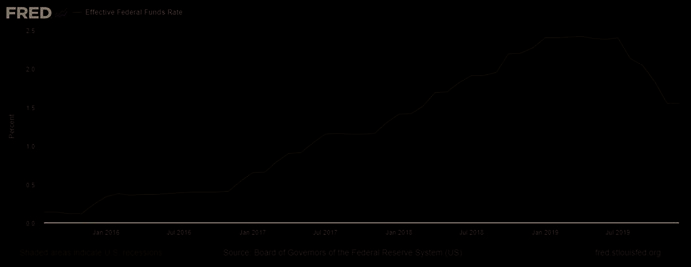
\includegraphics[width=0.8\textwidth]{gfx/m1l2_liq_exhibit3-1_fed_funds_rate.jpg}
    \caption{Lịch sử lãi suất Quỹ Liên bang (2015-2019)}
    \label{fig:fed_funds_rate}
\end{figure}

Dựa trên kỳ vọng của thị trường vào đầu tháng 10 năm 2018, những phát biểu của Chủ tịch Fed đã gây sốc cho hầu hết các nhà đầu tư. Họ lo sợ Fed có thể đang quá quyết liệt trong chính sách tiền tệ thắt chặt của mình và cuối cùng có thể đẩy nền kinh tế vào suy thoái. Do đó, lợi suất trái phiếu Kho bạc Hoa Kỳ kỳ hạn 10 năm (10-year U.S. Treasury note yields) ban đầu nhảy vọt lên 3,21\% sau thông báo, trước khi giảm xuống 2,69\% vào cuối năm 2018, trong khi chứng khoán sụt giảm 14\% trong suốt quý IV. Nỗi lo ngại về một cuộc suy thoái đã thúc đẩy những phản ứng mạnh mẽ này và tạo ra một mức độ biến động giá rất lớn trên thị trường trái phiếu và cổ phiếu. Hình 3.2 hiển thị lộ trình lợi suất trái phiếu Kho bạc trong năm 2018-2019, và Hình 3.3 hiển thị chỉ số thị trường chứng khoán S\&P 500 trong cùng khoảng thời gian này.

\begin{figure}[htbp]
    \centering
    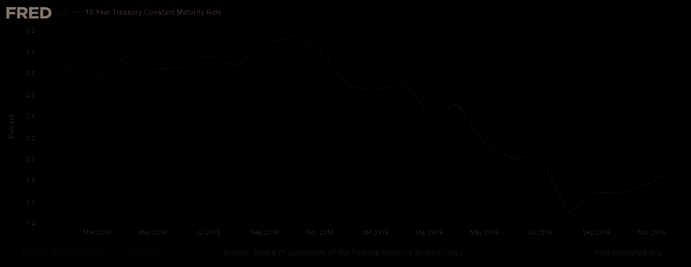
\includegraphics[width=0.8\textwidth]{gfx/m1l2_liq_exhibit3-2_treasury_yields.jpg}
    \caption{Lợi suất trái phiếu Kho bạc Hoa Kỳ kỳ hạn 10 năm (2018-2019)}
    \label{fig:treasury_yields}
\end{figure}

\begin{figure}[htbp]
    \centering
    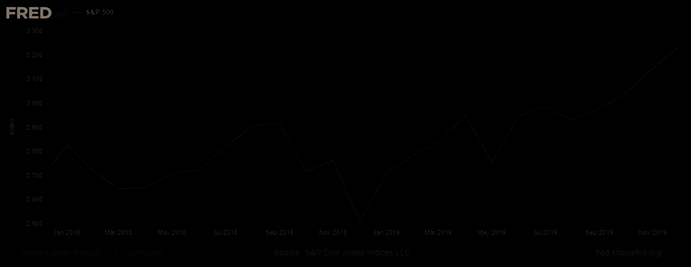
\includegraphics[width=0.8\textwidth]{gfx/m1l2_liq_exhibit3-3_sp500_longterm.jpg}
    \caption{Chỉ số thị trường chứng khoán S\&P 500 - Biến động dài hạn (2018-2019)}
    \label{fig:sp500_longterm}
\end{figure}

Hình 3.2 và 3.3 cung cấp những minh họa sống động về cách thức các thị trường tài chính tương tác với kinh tế vĩ mô theo hướng mà cả hai bên cùng ảnh hưởng lẫn nhau. Điều này có thể được nhìn thấy không chỉ ở sự sụt giảm nhanh chóng của lợi suất trái phiếu và giá cổ phiếu trong năm 2018, mà còn ở những phản ứng tích cực đối với các tuyên bố và hành động sau đó của Fed trong năm 2019, khi họ bắt đầu tạm dừng và cuối cùng là hạ lãi suất Quỹ Liên bang. Sau khi làm thị trường tài chính hoảng sợ ban đầu vào năm 2018, các hành động của Fed đã châm ngòi cho những đợt tăng điểm (rallies) lớn ở cả giá cổ phiếu và trái phiếu trong năm 2019.\footnote{Lưu ý rằng giá trái phiếu di chuyển ngược chiều với những thay đổi về lãi suất, do đó sự sụt giảm mạnh của lợi suất trái phiếu Kho bạc Hoa Kỳ kỳ hạn 10 năm từ mức hơn 3,2\% vào tháng 10 năm 2018 xuống còn 1,5\% vào tháng 8 năm 2019 đã tạo ra mức lợi nhuận vốn (capital gains) khổng lồ cho các nhà đầu tư trái phiếu.} Xuyên suốt quá trình này, các thành viên tham gia thị trường liên tục đánh giá bất kỳ thông tin mới nào về xu hướng của Fed, và bản thân Fed cũng theo dõi chặt chẽ các phản ứng của thị trường đối với những thay đổi trong chính sách tiền tệ của mình.

Chúng ta cũng có thể "phóng to" để kiểm tra xem thị trường chứng khoán đã phản ứng như thế nào với những bình luận của Chủ tịch Fed bằng cách nhìn vào các mức giá trong ngày (intraday prices) xung quanh những ngày diễn ra các tuyên bố này. Biến động giá trong ngày vào các ngày từ 3 đến 5 tháng 10 năm 2018 của chỉ số S\&P 500 được trình bày dưới đây.

\begin{figure}[htbp]
    \centering
    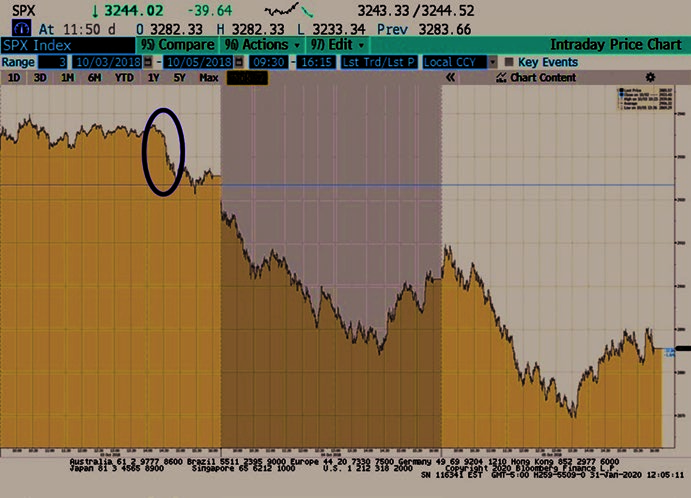
\includegraphics[width=0.8\textwidth]{gfx/m1l2_liq_exhibit3-4_sp500_intraday_oct3-5.jpg}
    \caption{Chỉ số thị trường chứng khoán S\&P 500 - Biến động trong ngày (3 tháng 10, 2018 - 5 tháng 10, 2018)}
    \label{fig:sp500_intraday_oct3-5}
\end{figure}

Như có thể thấy từ Hình 3.4, có một phản ứng mạnh mẽ và nhanh chóng đối với những bình luận bất ngờ của Chủ tịch Powell về việc cần phải tiếp tục tăng lãi suất. Cần lưu ý rằng phản ứng bắt đầu diễn ra vào buổi chiều ngày 3 tháng 10 ngay sau khi các bình luận của chủ tịch được công bố (được đánh dấu trong biểu đồ bằng hình bầu dục). Khi thị trường đạt được hiệu quả thông tin, chúng ta sẽ kỳ vọng loại phản ứng nhanh chóng này đối với các tin tức bất ngờ. Như được hiển thị dưới đây trong Hình 3.5 cho một ngày duy nhất, cú rơi ban đầu diễn ra ngay lập tức và rất dốc (giảm 0,4\% từ đỉnh của thị trường lúc 2:15 chiều cho đến khi đóng cửa lúc 4:00 chiều ngày 3 tháng 10); đợt bán tháo của thị trường tiếp diễn trong các ngày 4-5 tháng 10, tạo ra tổng mức giảm 1,8\% so với đỉnh trước thông báo\footnote{Nếu đợt sụt giảm trong hơn 2 ngày này được tính theo tỷ lệ hàng năm (annualized), khoản lỗ lũy kế sẽ xấp xỉ 84\% giá trị ban đầu của một nhà đầu tư sau 1 năm.}, do những thành viên tham gia thị trường lúc này đã xử lý đầy đủ các hệ lụy từ khả năng lãi suất tiếp tục tăng đối với nền kinh tế và các thị trường tài chính. 

\begin{figure}[htbp]
    \centering
    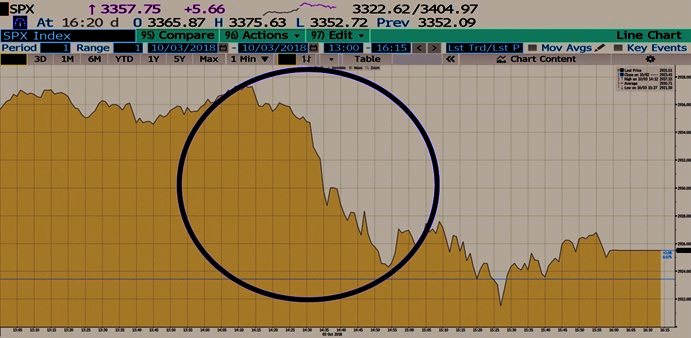
\includegraphics[width=0.8\textwidth]{gfx/m1l2_liq_exhibit3-5_sp500_intraday_oct3.jpg}
    \caption{Chỉ số thị trường chứng khoán S\&P 500 - Biến động trong ngày (3 tháng 10, 2018)}
    \label{fig:sp500_intraday_oct3}
\end{figure}

Bằng cách phóng to hơn nữa, chúng ta có thể thấy qua vòng tròn trong Hình 3.5 rằng phần lớn phản ứng ban đầu của chỉ số S\&P 500 xảy ra từ 2:15 chiều đến 2:55 chiều. Kiểu hình (pattern) này thường xuất hiện khi phản ứng ban đầu của thị trường tài chính là nhanh chóng và mạnh mẽ, nhưng như biểu đồ trước đó ở Hình 3.4 cho thấy, xu hướng giá có thể tiếp diễn trong nhiều ngày khi quá trình hài hòa giữa các kỳ vọng phân kỳ thông qua giao dịch giữa "phe bò" (bulls) và "phe gấu" (bears) dần được bộc lộ.

Trái ngược với hành vi của thị trường chứng khoán vào tháng 10 năm 2018 được hiển thị ở trên, chúng ta cũng có thể xem xét một phản ứng mạnh và nhanh khác, nhưng lần này là theo chiều ngược lại của chỉ số S\&P 500. Như đã lưu ý trước đó, thị trường phản ứng tích cực với các bình luận ôn hòa hơn của Powell liên quan đến việc tạm dừng các đợt tăng lãi suất tiềm năng trong tương lai vào đầu năm 2019. Phản ứng này có thể được nhìn thấy trong Hình 3.6 thông qua các mô hình giá trong ngày đối với chỉ số chứng khoán chính yếu này trong hai ngày 3-4 tháng 1 năm 2019.

\begin{figure}[htbp]
    \centering
    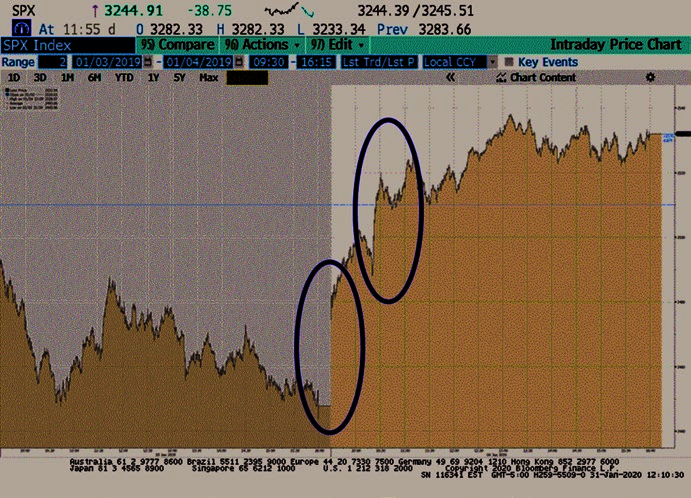
\includegraphics[width=0.8\textwidth]{gfx/m1l2_liq_exhibit3-6_sp500_intraday_jan3-4.jpg}
    \caption{Chỉ số thị trường chứng khoán S\&P 500 - Biến động trong ngày (3 tháng 1, 2019 - 4 tháng 1, 2019)}
    \label{fig:sp500_intraday_jan3-4}
\end{figure}

Hình 3.6 cho thấy một cú nhảy vọt lớn vào sáng sớm ngày 4 tháng 1 năm 2019 (xem hình bầu dục đầu tiên trên biểu đồ). Phản ứng tích cực ban đầu khi thị trường mở cửa lúc 9:30 sáng là do một báo cáo về việc làm phi nông nghiệp (nonfarm employment report) mạnh mẽ một cách đáng ngạc nhiên được công bố sớm hơn vào sáng hôm đó lúc 8:30 sáng, cho thấy 312.000 việc làm đã được tạo ra ở Hoa Kỳ trong tháng 12 năm 2018. Ngay khi thị trường chứng khoán mở cửa trở lại lúc 9:30 sáng ngày 4 tháng 1, chỉ số chứng khoán S\&P 500 đã tăng vọt lên 2.475,90 (mức tăng 1,1\% so với mức đóng cửa của ngày hôm trước là 2.447,89). Cú nhảy lớn và không liên tục này từ mức giá đóng cửa trước đó được gọi là "gap up" (tạo khoảng trống giá lên) trong ngôn ngữ của phân tích kỹ thuật. Đây là một ví dụ kinh điển về cách các thị trường tài chính phản ứng nhanh chóng với những tin tức tích cực bất ngờ về kinh tế vĩ mô.

Thị trường chứng khoán sau đó đã nhảy vọt lần thứ hai vào cuối buổi sáng hôm đó, giữa 10:00 sáng và 11:00 sáng, do Chủ tịch Powell tuyên bố rằng Fed đang cân nhắc việc tạm dừng các đợt tăng lãi suất Quỹ Liên bang trong tương lai. Giống như mô hình (pattern) được hiển thị trước đó trong Hình 3.4 và 3.5, các bình luận công khai của Chủ tịch về chính sách tiền tệ là nằm ngoài dự đoán, và do đó, các nhà giao dịch và nhà đầu tư đã phản ứng nhanh chóng, như có thể thấy ở hình bầu dục thứ hai trên Hình 3.6. Hiệu ứng ròng (net effect) đối với giá cổ phiếu là cực kỳ nhanh và lớn. Sau đó, chỉ số này tiếp tục xu hướng đi lên trong phần còn lại của ngày và đóng cửa ở mức 2.531,94, tạo ra mức lợi nhuận tổng cộng 3,02\% so với mức đóng cửa của ngày hôm trước. Đây là một mức tăng rất lớn vì các chỉ số thị trường chứng khoán của Hoa Kỳ thông thường biến động dưới 1\% mỗi ngày.

Hình 3.7 cho thấy sự khác biệt về thanh khoản của các chứng khoán cá nhân có thể ảnh hưởng đến quá trình khám phá giá như thế nào xung quanh các bình luận của Chủ tịch Powell vào ngày 4 tháng 1 năm 2019. Để minh họa hai cổ phiếu có thể phản ứng theo những cách rất khác nhau đối với cùng một tin tức từ Chủ tịch Fed, Hình 3.7 hiển thị các mô hình giá trong ngày từ 9:30 sáng đến 11:15 sáng hôm đó đối với một cổ phiếu có tính thanh khoản rất cao là Microsoft (một gã khổng lồ phần mềm toàn cầu), và một cổ phiếu có tính thanh khoản khá kém là Flushing Financial (một ngân hàng thương mại nhỏ có trụ sở tại Thành phố New York). Đường màu trắng trích xuất những biến động của cổ phiếu Microsoft, trong khi đường đứt nét biểu thị các chuyển động của Flushing Financial.\footnote{Cả hai cổ phiếu đều đã được lập chỉ mục (indexed) đến giá trị cơ sở ban đầu là 100 để dễ so sánh.} Có thể nhận thấy rằng mô hình giá của Microsoft trơn tru hơn rất nhiều vì các giao dịch xảy ra thường xuyên và ở các mức giá khá gần với các mức giá trước đó. Do vậy, bất chấp tin tức lớn từ Fed trong ngày hôm đó, cổ phiếu của Microsoft vẫn phản ứng nhanh chóng và theo một cách "công bằng và có trật tự" vì nhiều giao dịch đã được thực hiện liên tục trong từng phút giao dịch.

\begin{figure}[htbp]
    \centering
    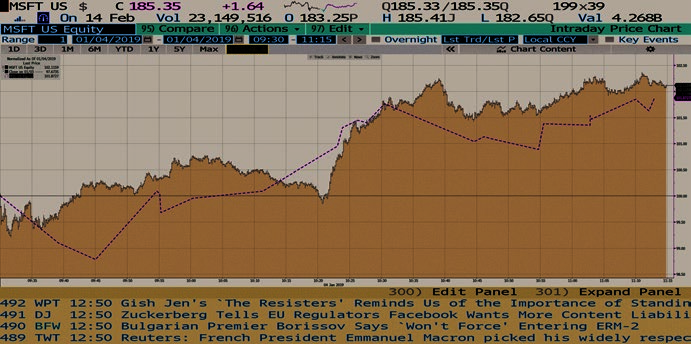
\includegraphics[width=0.8\textwidth]{gfx/m1l2_liq_exhibit3-7_large_vs_small_cap.jpg}
    \caption{Biến động trong ngày của Cổ phiếu vốn hóa lớn so với Cổ phiếu vốn hóa nhỏ (4 tháng 1, 2019)}
    \label{fig:large_vs_small_cap}
\end{figure}

Trái ngược lại, đường đứt nét của Flushing Financial di chuyển theo một cách thức đột ngột và lởm chởm vì cổ phiếu của nó không giao dịch thường xuyên đến vậy. Điều này cũng dẫn đến việc giá cổ phiếu bị tụt hậu (lag) so với những biến động của chỉ số thị trường chứng khoán S\&P 500 và của Microsoft. Trên thực tế, trong khoảng thời gian 9:30-11:15 sáng của ngày hôm đó, cổ phiếu Flushing Financial chỉ giao dịch vỏn vẹn 25 lần, trong khi Microsoft được giao dịch tới 2.520 lần! Hơn nữa, tổng khối lượng giao dịch cổ phiếu hàng ngày (daily share trading volume) đối với Microsoft là 44.061.000, và đối với Flushing Financial chỉ là 67.250.

Điều này thể hiện một sự khác biệt rất lớn về hoạt động giao dịch, trong đó cổ phiếu của Microsoft có tính thanh khoản cao hơn hẳn, do người mua và người bán có thể dễ dàng giao dịch vào bất kỳ thời điểm nào trong phiên giao dịch (ví dụ: trung bình 24 lần mỗi phút). Ngược lại, cổ phiếu của Flushing Financial không giao dịch quá thường xuyên trong khoảng thời gian này (một lần mỗi 4,2 phút), và do đó, giá của nó buộc phải dịch chuyển mạnh hơn vào thời điểm nó thực sự có giao dịch nhằm "bắt kịp" với các tin tức về báo cáo việc làm của Hoa Kỳ và các bình luận của Chủ tịch Fed. Do đó, việc khám phá ra mức giá "chính xác" đối với một cổ phiếu kém thanh khoản như Flushing Financial khó khăn hơn rất nhiều vì thiếu các giao dịch thường xuyên. Mặc dù biểu đồ này chỉ cho thấy hai cổ phiếu, những sự khác biệt về thanh khoản như vậy tồn tại ở hàng nghìn cổ phiếu được giao dịch tại Hoa Kỳ trong bất kỳ ngày nào.

Cơ chế giao dịch và quá trình khám phá giá được mô tả trước đó trong chương này là những công cụ thiết yếu cần có nhằm tạo thuận lợi cho những tương tác này giữa kinh tế vĩ mô và thị trường tài chính. Do vậy, việc sở hữu những thị trường tài chính hoạt động tốt và có tính thanh khoản cao là vô cùng quan trọng, giúp các tín hiệu giữa các nhà hoạch định chính sách, nhà đầu tư, giám đốc kinh doanh và người tiêu dùng trở nên rõ ràng nhất có thể.



% ---- Lesson 3: Government Bond Yield Curve Analysis ----
% Thứ tự đọc: Lesson Notes (trong VM, xem ghi chú trong chương) -> Đọc thêm
\chapter{Đường cong Lợi suất Trái phiếu Chính phủ}
\label{ch:M1L3}

\section*{Lesson Notes}

\textbf{Dự án} \\
\textbf{Thời gian đọc:} 60 phút \\
\textbf{Kiến thức nền tảng:} Trái phiếu Kho bạc Hoa Kỳ (U.S. Treasury Bonds), Đường cong lợi suất (Yield Curve), Đại số tuyến tính (Linear Algebra), Python cơ bản \\
\textbf{Từ khóa:} Đường cong giá-lợi suất trái phiếu (Bond price-yield curve), Lãi suất phi rủi ro (Risk free interest rate), Nelson Siegel, Spline bậc ba (Cubic Spline)

Trong bài học trước, chúng ta đã tìm hiểu cách lấy thông tin về lợi suất Trái phiếu Kho bạc Hoa Kỳ và đi qua một số khái niệm nền tảng về đường cong lợi suất. Trong bài học này, chúng ta sẽ đi sâu hơn và tìm hiểu cách khớp (fit) một đường cong lợi suất trái phiếu. Chúng ta sẽ tiếp tục sử dụng dữ liệu lợi suất Trái phiếu Kho bạc Hoa Kỳ để làm ví dụ minh họa.

\section[Lãi suất Phi rủi ro]{Lãi suất Phi rủi ro (Risk-Free Interest Rates)}

Trong khóa học Thị trường Tài chính, chúng ta đã tìm hiểu về rủi ro tín dụng khi đầu tư vào trái phiếu. Rủi ro tín dụng, được gánh chịu bởi nhà đầu tư trái phiếu, là rủi ro mà tổ chức phát hành trái phiếu sẽ vỡ nợ (default). Một thực thể có xếp hạng tín dụng hoặc điểm tín dụng cao có thể vay tiền từ các thị trường tài chính với mức lãi suất thấp hơn so với một thực thể có xếp hạng tín dụng thấp hơn. Tại Hoa Kỳ, các trái phiếu do chính phủ phát hành (Trái phiếu Kho bạc Hoa Kỳ hay Treasuries) thường được coi là trái phiếu có xếp hạng tín dụng cao. Do đó, lợi suất Trái phiếu Kho bạc thường được sử dụng làm lãi suất phi rủi ro cho việc định giá trái phiếu trong ngành tài chính. Có rất nhiều cuộc tranh luận về việc liệu Trái phiếu Kho bạc Hoa Kỳ có thực sự an toàn với rủi ro vỡ nợ bằng không hay không. Những kịch bản khác nhau sẽ cần những cân nhắc khác nhau. Trong bài học này, chúng ta sẽ tuân theo quy ước hiện hành của thị trường tài chính bằng cách sử dụng lợi suất Trái phiếu Kho bạc Hoa Kỳ làm lãi suất phi rủi ro.

Một khái niệm quan trọng khác trong rủi ro tín dụng là phần bù rủi ro tín dụng (credit spread). Chênh lệch tín dụng hay phần bù tín dụng là khoảng chênh lệch lãi suất giữa một trái phiếu doanh nghiệp và một trái phiếu chính phủ có cùng kỳ hạn. Khoảng chênh lệch lãi suất này cũng được gọi là lợi suất vượt trội (excess return) của trái phiếu doanh nghiệp vì lợi suất trái phiếu chính phủ là lãi suất phi rủi ro. Lợi suất vượt trội của trái phiếu doanh nghiệp là phần lợi nhuận tăng thêm dành cho người nắm giữ trái phiếu doanh nghiệp để họ chấp nhận gánh chịu rủi ro bổ sung khi nắm giữ trái phiếu này.

Vì lãi suất phi rủi ro là một yếu tố then chốt không chỉ trong định giá trái phiếu mà còn trong định giá các tài sản tài chính khác và quản lý danh mục đầu tư, nên việc hiểu được các đặc điểm và hành vi của lãi suất phi rủi ro là vô cùng quan trọng. Trong bài học này, chúng ta sẽ sử dụng lợi suất trái phiếu (hay các trái phiếu) kho bạc Hoa Kỳ làm lãi suất phi rủi ro để điều tra hành vi của chúng và tiến hành phân tích.

\section[Biến động của Lợi suất Trái phiếu Kho bạc Hoa Kỳ]{Biến động của Lợi suất Trái phiếu Kho bạc Hoa Kỳ (Volatility of U.S. Treasury Yields)}

Đầu tiên, hãy xem xét các mức độ biến động của lợi suất Trái phiếu Kho bạc ở các kỳ hạn khác nhau. Chúng ta tiếp tục phương pháp của Bài 2 để lấy dữ liệu lợi suất Trái phiếu Kho bạc từ FRED bằng Python như sau.

\begin{lstlisting}[language=Python]
In [1]: import pandas as pd
        from fredapi import Fred
        import matplotlib.pyplot as plt
        import seaborn as sns
        sns.set()
\end{lstlisting}

\begin{lstlisting}[language=Python]
In [2]: # Initialize the FRED API with your key
        fred = Fred(api_key='5079f41d061a4037d81f3da69e018803') # Replace my APIKEY
        
        # List of Treasury yield series IDs
        series_ids = ['DGS1MO', 'DGS3MO', 'DGS6MO', 'DGS1', 'DGS2', 'DGS3', 'DGS5',
                      'DGS7', 'DGS10', 'DGS20', 'DGS30']
                      
        # Function to get data for a single series
        def get_yield_data(series_id):
            data = fred.get_series(series_id, observation_start="1975-01-01", observ
            return data
            
        #Get data for all series
        yields_dict = {series_id: get_yield_data(series_id) for series_id in series_
        
        # Combine into a single DataFrame
        yields = pd.DataFrame(yields_dict)
        
        # Rename columns for clarity
        yields.columns = ['1 Month', '3 Month', '6 Month', '1 Year', '2 Year', '3 Ye
                          '7 Year', '10 Year', '20 Year', '30 Year']
\end{lstlisting}

\begin{lstlisting}[language=Python]
In [3]: yields.index = pd.to_datetime(yields.index)
\end{lstlisting}

Bây giờ chúng ta hãy tính độ lệch chuẩn của lợi suất Trái phiếu Kho bạc ở các kỳ hạn khác nhau. Sau đó, chúng ta sẽ vẽ một đồ thị để trình bày các độ lệch chuẩn theo kỳ hạn.

\begin{lstlisting}[language=Python]
In [4]: yields = yields.dropna()
        y_std = yields.std()
        y_std
\end{lstlisting}

\begin{lstlisting}[language=Python]
Out [4]: 1 Month    1.705851
         3 Month    1.733347
         6 Month    1.746829
         1 Year     1.684091
         2 Year     1.545413
         3 Year     1.446639
         5 Year     1.309345
         7 Year     1.226457
         10 Year    1.174092
         20 Year    1.206514
         30 Year    1.108774
         dtype: float64
\end{lstlisting}

\begin{lstlisting}[language=Python]
In [5]: fig, ax = plt.subplots()
        y_std.plot(figsize=(8,5), marker='o', title='Figure 0, Standard Deviations
        plt.xlabel("Maturity")
        plt.ylabel("Standard Deviation")
        
        for i in range(len(y_std)):
            ax.annotate(str(round(y_std.iloc[i], 2)), xy=(i,y_std.iloc[i]))
            
        plt.show()
\end{lstlisting}

\begin{figure}[htbp]
    \centering
    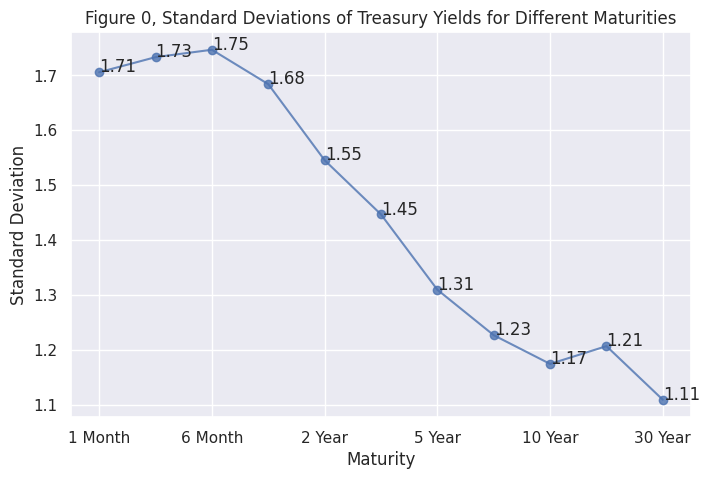
\includegraphics[width=0.8\textwidth]{gfx/m1l3_notes_fig0_std_deviations.png}
    \caption{Hình 0, Độ lệch chuẩn của Lợi suất Trái phiếu Kho bạc theo các Kỳ hạn khác nhau}
    \label{fig:m1l3_fig0}
\end{figure}

Từ đồ thị trên, chúng ta thấy rằng độ lệch chuẩn của trái phiếu Kho bạc Hoa Kỳ có kỳ hạn ngắn cao hơn so với trái phiếu Kho bạc Hoa Kỳ có kỳ hạn dài hơn. Độ lệch chuẩn đối với các trái phiếu Kho bạc có kỳ hạn dưới một năm duy trì ở mức cao trên 1,7. Sau đó, độ lệch chuẩn của các trái phiếu Kho bạc có kỳ hạn trên một năm giảm đều.

\section[Đường cong Giá - Lợi suất Trái phiếu Kho bạc]{Đường cong Giá - Lợi suất Trái phiếu Kho bạc (Treasury Bond Price-Yield Curve)}

Theo công thức toán học về giá trái phiếu, mối quan hệ giữa giá trái phiếu và lợi suất trái phiếu là phi tuyến. Mối quan hệ này được giải thích tốt nhất thông qua đường cong giá - lợi suất trái phiếu. Hãy sử dụng hình sau đây để minh họa mối quan hệ này.

\textbf{Hình 1: Đường cong Giá - Lợi suất Trái phiếu} \\
\textit{Đồ thị thể hiện giá so với lợi suất với một đường thẳng cắt một đường cong tại một điểm được đánh dấu}

Trong Hình 1, chúng ta có thể thấy rằng khi lợi suất/lãi suất của một trái phiếu tăng, giá của trái phiếu sẽ giảm. Ngược lại, khi lợi suất/lãi suất của trái phiếu giảm, giá của trái phiếu sẽ tăng. Có một mối quan hệ nghịch biến giữa giá trái phiếu và lợi suất trái phiếu. Tuy nhiên, khi lợi suất thay đổi một đơn vị, mức độ thay đổi của giá sẽ khác nhau tùy thuộc vào việc mức lợi suất đang ở đâu khi sự thay đổi lợi suất xảy ra.

Đây là một điểm then chốt khác cần chú ý trong mối quan hệ giá - lợi suất trái phiếu: giá trái phiếu và lợi suất trái phiếu không có mối quan hệ tuyến tính; chúng có mối quan hệ lồi (convex). Mối quan hệ phi tuyến giữa giá trái phiếu và lợi suất trái phiếu có ý nghĩa quan trọng trong quản trị rủi ro lãi suất đối với đầu tư trái phiếu. Hãy sử dụng Hình 2 sau đây để giải thích khái niệm này.

\textbf{Hình 2: Mối quan hệ Phi tuyến giữa Giá Trái phiếu và Lợi suất Trái phiếu} \\
\textit{Đồ thị thể hiện giá so với lợi suất với hai hình chữ nhật (D1, D2) minh họa sự thay đổi của giá (P1, P2) dọc theo một đường cong dốc xuống}

Dựa trên tính chất lồi của đường cong giá-lợi suất trái phiếu được mô tả trong Hình 2, mức độ thay đổi giá khi lợi suất thay đổi một lượng như nhau sẽ khác nhau tùy thuộc vào mức lợi suất. Trong Hình 2, D1 và D2 có cùng độ dài. Khi lợi suất thay đổi một khoảng D1, mức độ thay đổi giá là P1. Khi lợi suất thay đổi một khoảng D2, mức độ thay đổi giá là P2. Tuy nhiên, mức lợi suất cho D1 cao hơn mức lợi suất cho D2. Do tính lồi của đường cong giá-lợi suất, P1 nhỏ hơn P2.

Đặc tính này của mối quan hệ giữa giá trái phiếu và lợi suất trái phiếu được gọi là độ cong (curvature). Ví dụ trên chứng minh rằng độ dốc của đường cong giá-lợi suất thay đổi khi mức lợi suất thay đổi. Độ cong của đường cong giá-lợi suất được sử dụng để mô tả sự phụ thuộc của độ dốc này vào mức lợi suất. Một nhà quản lý danh mục đầu tư trái phiếu sẽ phải chú ý đến độ cong của các khoản nắm giữ trái phiếu khi quản trị rủi ro lãi suất.

\section[Khớp Đa thức cho Đường cong Lợi suất Trái phiếu Kho bạc Hoa Kỳ]{Khớp Đa thức cho Đường cong Lợi suất Trái phiếu Kho bạc Hoa Kỳ (Polynomial Fitting for U.S. Treasury Yield Curve)}

Chúng ta đã nói về đường cong lợi suất Trái phiếu Kho bạc Hoa Kỳ trong bài học trước. Đường cong lợi suất mô tả mối quan hệ giữa lợi suất trái phiếu và thời gian đáo hạn (hay kỳ hạn) của các trái phiếu tương tự. Mối quan hệ này cũng được gọi là cấu trúc kỳ hạn (term structure) của một đường cong lợi suất. Phân tích cấu trúc kỳ hạn đóng vai trò quan trọng trong việc định giá trái phiếu và quản trị rủi ro lãi suất. Trong phần này, chúng ta sẽ giới thiệu các phương pháp để khớp (fit) một đường cong lợi suất. Chúng ta sẽ tiếp tục sử dụng lợi suất trái phiếu Kho bạc Hoa Kỳ làm ví dụ. Đầu tiên, hãy vẽ một đồ thị cho đường cong lợi suất Trái phiếu Kho bạc Hoa Kỳ vào ngày 10 tháng 1 năm 2020.

\begin{lstlisting}[language=Python]
In [6]: def plot_yield_curve(date, fig_n):
            maturities = ['1M', '3M', '6M', '1Y', '2Y', '3Y', '5Y', '7Y', '10Y', '20
            fig, ax = plt.subplots(figsize=(12, 6))
            ax.plot(maturities, yields.loc[date], marker='D', label='Yield Curve at 
            
            ax.set_yticklabels(['{:.2f}%'.format(y) for y in ax.get_yticks()])
            ax.set_xticks(range(len(maturities)))
            ax.set_xticklabels(maturities)
            
            # Add labels and title
            ax.set_xlabel('Maturity')
            ax.set_ylabel('Yield')
            ax.set_title(fig_n+'Treasury Yield Curve')
            
            fig.legend(loc = [0.69, 0.14])
            
            # Show the plot
            plt.grid(True)
            plt.show()

        print("Figure 3")
        plot_yield_curve('2020-01-10', 'Figure 3, ')
\end{lstlisting}

\begin{lstlisting}[language=Python]
Figure 3
/tmp/ipykernel_18/1226209266.py:6: UserWarning: set_ticklabels() should only
be used with a fixed number of ticks, i.e. after set_ticks() or using a Fixe
dLocator.
  ax.set_yticklabels(['{:.2f}%'.format(y) for y in ax.get_yticks()])
\end{lstlisting}

\begin{figure}[htbp]
    \centering
    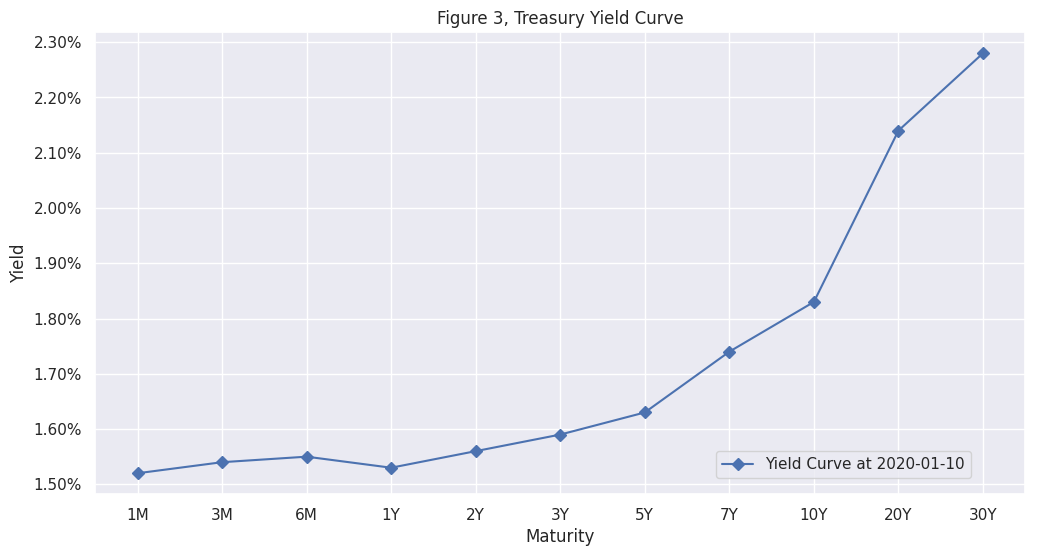
\includegraphics[width=0.8\textwidth]{gfx/m1l3_notes_fig3_yield_curve_2020-01-10.png}
    \caption{Hình 3, Đường cong Lợi suất Trái phiếu Kho bạc}
    \label{fig:m1l3_fig3}
\end{figure}

Trong phần này, chúng ta sẽ sử dụng kỹ thuật khớp đa thức (polynomial fitting) để ước tính một đường cong lợi suất.

Khớp đa thức là khi một nhà nghiên cứu sử dụng các đa thức bậc $n$ của biến đầu vào để dự đoán biến đầu ra. Ví dụ, nếu biến đầu vào là $x$ và biến đầu ra là $y$, biểu thức sau đây sẽ sử dụng các đa thức bậc $n$ của $x$ để dự đoán $y$.

$$y=\beta_{0}+\beta_{1}x_{1}+\beta_{2}x^{2}+\beta_{3}x^{3}...+\beta_{n}x^{n}$$

$\beta_{0},\beta_{1},\beta_{2},\beta_{3},...,\beta_{n}$ là các tham số cần được ước tính.
Có một số phương pháp khớp đa thức để khớp một đường cong lợi suất. Trong bài học này, chúng ta sẽ học hai phương pháp: mô hình Nelson Siegel và khớp spline bậc ba.

\subsection[Mô hình Nelson Siegel]{Mô hình Nelson Siegel (Nelson Siegel Model)}

Mô hình Nelson Siegel (mô hình NS) là một mô hình phổ biến để mô tả mối quan hệ giữa kỳ hạn và lợi suất (Svensson). Dưới đây là công thức của mô hình:

$$y(t)=\beta_{0}+\beta_{1}\left(\frac{1-e^{-\lambda t}}{\lambda t}\right)+\beta_{2}\left(\frac{1-e^{-\lambda t}}{\lambda t}-e^{-\lambda t}\right)+\epsilon$$

$\beta_{0},\beta_{1},\beta_{2}$ là các tham số cần được ước tính. $t$ là thời gian đáo hạn và $\lambda$ là tốc độ phân rã (decay rate). Tốc độ phân rã nằm trong khoảng từ 0 đến 1.
$\beta_{0}$ được dùng để mô tả mức độ (level) của đường cong lợi suất. $\beta_{1}$ được dùng để mô tả độ dốc (slope) của đường cong lợi suất và $\beta_{2}$ được dùng để mô tả hình dạng (shape) của đường cong lợi suất. Vì lý do này, chúng ta cũng gọi mô hình NS là mô hình nhân tố đường cong lợi suất.
Mô hình NS phân tách đường cong lợi suất thành ba phần tử như mô tả ở trên.
Tốc độ phân rã hoạt động như thế nào? Tốc độ phân rã càng nhỏ, đường cong phân rã càng chậm. Tốc độ phân rã càng lớn, đường cong phân rã càng nhanh. Tốc độ phân rã cho thấy lợi suất sẽ hội tụ nhanh đến mức nào về mức trung bình dài hạn.

Với cấu trúc đơn giản của mô hình NS, chúng ta có thể sử dụng các phần tử khác nhau trong mô hình để mô tả các hành vi khác nhau của đường cong lợi suất. Một khi chúng ta có được một ước lượng mô hình NS, chúng ta có thể sử dụng mô hình này để dự đoán diễn biến của những thay đổi lãi suất trong tương lai (Pape).

Hãy sử dụng gói Nelson Siegel Sevensson từ Python để chứng minh mô hình NS.

\subsection[Mô hình Nelson Siegel: Ứng dụng Python]{Mô hình Nelson Siegel: Ứng dụng Python (Nelson Siegel Model: Python Demonstration)}

Trong phần này, chúng ta sẽ sử dụng gói Nelson Siegel Sevensson từ Python để chỉ ra cách khớp một đường cong lợi suất. Đầu tiên, chúng ta cần cài đặt và import gói này.

\begin{lstlisting}[language=Python]
In [7]: pip install nelson_siegel_svensson
\end{lstlisting}

\begin{lstlisting}[language=Python]
Collecting nelson_siegel_svensson
  Downloading nelson_siegel_svensson-0.5.0-py2.py3-none-any.whl.metadata (6.
7 kB)
Collecting Click>=8.0 (from nelson_siegel_svensson)
  Downloading click-8.3.1-py3-none-any.whl.metadata (2.6 kB)
Requirement already satisfied: numpy>=1.22 in /usr/local/lib/python3.11/site
-packages (from nelson_siegel_svensson) (2.1.3)
...
Installing collected packages: Click, nelson_siegel_svensson
Successfully installed Click-8.3.1 nelson_siegel_svensson-0.5.0
WARNING: Running pip as the 'root' user can result in broken permissions and
conflicting behaviour with the system package manager, possibly rendering yo
ur system unusable. It is recommended to use a virtual environment instead:
https://pip.pypa.io/warnings/venv. Use the root-user-action option if you
know what you are doing and want to suppress this warning.
[notice] A new release of pip is available: 25.0.1 -> 25.3
[notice] To update, run: pip install --upgrade pip
Note: you may need to restart the kernel to use updated packages.
\end{lstlisting}

\begin{lstlisting}[language=Python]
In [8]: # Import the packages for fitting NS model
        from nelson_siegel_svensson.calibrate import calibrate_ns_ols
        import numpy as np
\end{lstlisting}

Sau khi import các gói cần thiết để khớp mô hình NS, chúng ta cần tạo các biến số cho việc lập mô hình. Đầu tiên chúng ta cần tạo một biến số kỳ hạn $t$ theo đơn vị năm. Ví dụ, 1 tháng là 0.08333 năm và 3 tháng là 0.25 năm. Biến số tiếp theo là biến số lợi suất. Cả biến kỳ hạn và biến lợi suất cần phải ở dưới dạng mảng (array form). Chúng ta sẽ sử dụng lợi suất từ ngày 10 tháng 1 năm 2020 (2020-01-10) làm ví dụ vì chúng ta vừa vẽ biểu đồ đường cong lợi suất vào ngày đó ở phần trước.

\begin{lstlisting}[language=Python]
In [9]: # Create maturity and yield variables in array form
        t = np.array([0.08333,0.25,0.5,1,2,3,5,7,10,20,30])
        y = np.array(yields.loc["2020-01-10"])
\end{lstlisting}

Sau khi các biến đã sẵn sàng, chúng ta có thể chuyển sang ước tính mô hình NS.

\begin{lstlisting}[language=Python]
In [10]: # Fit an NS model for yields from 2020-01-10
         curve, status = calibrate_ns_ols(t, y, tau0=1.0) # starting value of 1.0 fc
         assert status.success
         print(curve)
\end{lstlisting}

\begin{lstlisting}[language=Python]
NelsonSiegelCurve(beta0=np.float64(2.637682060451667), beta1=np.float64(-1.1
025872497097822), beta2=np.float64(-1.140646506802234), tau=np.float64(4.750
029828985478))
\end{lstlisting}

Kết quả của mô hình NS hiển thị $\beta_{0}$, $\beta_{1}$, $\beta_{2}$, và tốc độ phân rã đã được ước lượng. Bây giờ chúng ta hãy vẽ đồ thị để hiểu rõ hơn về kết quả mô hình.

\begin{lstlisting}[language=Python]
In [11]: y_hat = curve
         t_hat = np.linspace(0.5,30,100)
         plt.plot(t_hat, y_hat(t_hat))
         plt.xlabel("Maturity")
         plt.ylabel("Yield")
         plt.title("Figure 4, NS Model Result")
\end{lstlisting}

\begin{lstlisting}[language=Python]
Out [11]: Text(0.5, 1.0, 'Figure 4, NS Model Result')
\end{lstlisting}

\begin{figure}[htbp]
    \centering
    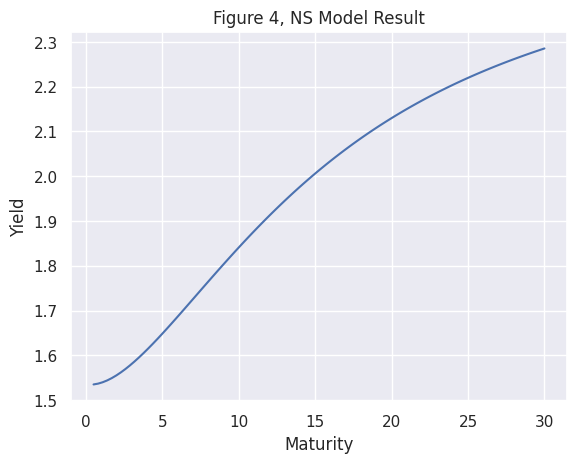
\includegraphics[width=0.8\textwidth]{gfx/m1l3_notes_fig4_ns_model_result.png}
    \caption{Hình 4, Kết quả Mô hình NS}
    \label{fig:m1l3_fig4}
\end{figure}

Từ Hình 4 ở trên, chúng ta có thể thấy đường cong lợi suất được ước tính khá khớp với biểu đồ đường cong mà chúng ta đã vẽ ở phần trước. Hãy thử ước tính một hình dạng khác của đường cong lợi suất. Lần này, chúng ta sẽ sử dụng lợi suất từ ngày 23 tháng 3 năm 2006 (2006-03-23). Trước tiên, hãy vẽ dữ liệu lợi suất từ 2006-03-23.

\begin{lstlisting}[language=Python]
In [12]: plot_yield_curve('2006-03-23', 'Figure 5, ')
\end{lstlisting}

\begin{lstlisting}[language=Python]
/tmp/ipykernel_18/1226209266.py:6: UserWarning: set_ticklabels() should only
be used with a fixed number of ticks, i.e. after set_ticks() or using a Fixe
dLocator.
  ax.set_yticklabels(['{:.2f}%'.format(y) for y in ax.get_yticks()])
\end{lstlisting}

\begin{figure}[htbp]
    \centering
    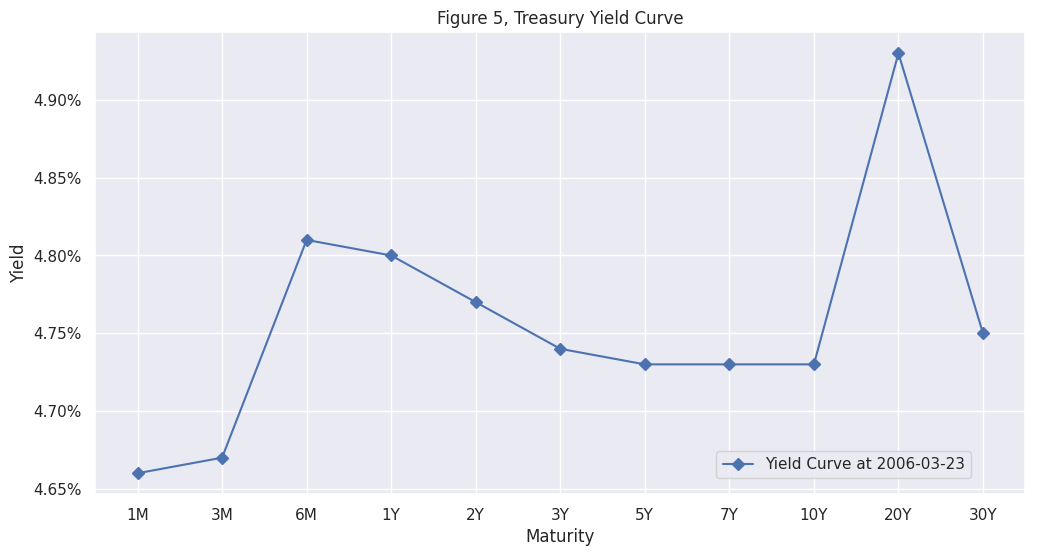
\includegraphics[width=0.8\textwidth]{gfx/m1l3_notes_fig5_yield_curve_2006-03-23.png}
    \caption{Hình 5, Đường cong Lợi suất Trái phiếu Kho bạc}
    \label{fig:m1l3_fig5}
\end{figure}

Trong Hình 5, các mức lợi suất từ kỳ hạn 6 tháng đến kỳ hạn 10 năm thể hiện hình dạng dốc xuống, điều này khác với đường cong lợi suất vào ngày 2020-01-10. Hãy xem liệu mô hình NS có nhận ra điều này hay không. Chúng ta sẽ lặp lại cùng quy trình đó để mô hình hóa đường cong lợi suất vào ngày 2006-03-23.

\begin{lstlisting}[language=Python]
In [13]: y = np.array(yields.loc["2006-03-23"])
         curve, status = calibrate_ns_ols(t, y, tau0=0.5) # starting value of 0.5 fo
         assert status.success
         print(curve)
\end{lstlisting}

\begin{lstlisting}[language=Python]
NelsonSiegelCurve(beta0=np.float64(4.7693015468990705), beta1=np.float64(-0.
1860856799305238), beta2=np.float64(0.25937117013919064), tau=np.float64(0.2
5704895433346897))
\end{lstlisting}

\begin{lstlisting}[language=Python]
In [14]: y_hat = curve
         t_hat = np.linspace(0.5,30,100)
         plt.plot(t_hat, y_hat(t_hat))
         plt.xlabel("Maturity")
         plt.ylabel("Yield")
         plt.title("Figure 6, NS Model Result")
\end{lstlisting}

\begin{lstlisting}[language=Python]
Out [14]: Text(0.5, 1.0, 'Figure 6, NS Model Result')
\end{lstlisting}

\begin{figure}[htbp]
    \centering
    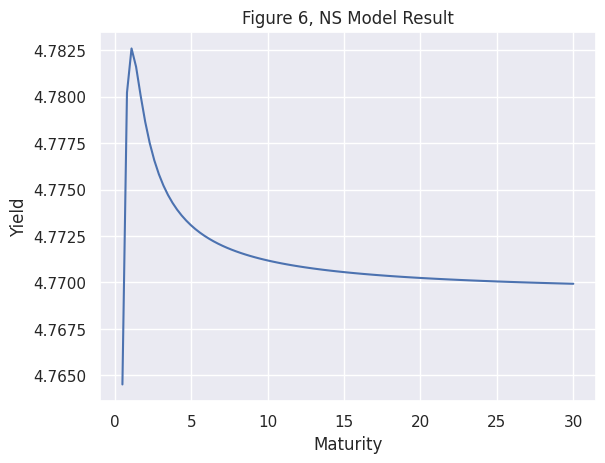
\includegraphics[width=0.8\textwidth]{gfx/m1l3_notes_fig6_ns_model_result2.png}
    \caption{Hình 6, Kết quả Mô hình NS}
    \label{fig:m1l3_fig6}
\end{figure}

Từ Hình 6 ở trên, chúng ta có thể thấy rằng đường cong dốc xuống sau một năm đáo hạn. Kết quả này nhất quán với Hình 5 mà chúng ta đã vẽ trước đó.

\section[Khớp Spline Bậc ba cho Đường cong Lợi suất]{Khớp Spline Bậc ba cho Đường cong Lợi suất (Cubic Spline Fitting of Yield Curve)}

Trong phần này, chúng ta sẽ giới thiệu một phương pháp phổ biến khác để khớp đường cong lợi suất với dữ liệu. Nó được gọi là spline bậc ba (cubic spline). Khớp spline là một phương pháp thuộc kỹ thuật khớp đa thức. Vui lòng đọc tài liệu bắt buộc "Phương pháp Nội suy Spline" để học lý thuyết về khớp spline, đặc biệt là khớp spline bậc ba. Chúng ta sẽ sử dụng phương pháp khớp spline bậc ba trong Python để khớp một đường cong lợi suất trong phần tiếp theo. Xin lưu ý rằng trong Bài 4 "Ứng dụng của Nội suy Spline Bậc hai", có một sai sót trong phần ghi chú. Trong ma trận lớn được trình bày, vector hệ số đáng lẽ phải nằm ở phía bên trái của phương trình, không phải ở phía bên phải.

\subsection[Ứng dụng Python: Sử dụng Khớp Spline Bậc ba để Khớp một Đường cong Lợi suất]{Ứng dụng Python: Sử dụng Khớp Spline Bậc ba để Khớp một Đường cong Lợi suất (Python Application: Use Cubic Spline Fitting to Fit a Yield Curve)}

Trong phần này, chúng ta sẽ chứng minh cách khớp một đường cong lợi suất bằng spline bậc ba. Để thuận tiện cho việc minh họa, chúng ta sẽ chỉ sử dụng lợi suất từ các Trái phiếu Kho bạc kỳ hạn 2 năm, 5 năm, 10 năm và 30 năm vào ngày 2020-01-10 làm ví dụ. Đầu tiên, hãy kiểm tra các lợi suất vào ngày 2020-01-10.

\begin{lstlisting}[language=Python]
In [15]: yields.loc["2020-01-10"]
\end{lstlisting}

\begin{lstlisting}[language=Python]
Out [15]: 1 Month     1.52
          3 Month     1.54
          6 Month     1.55
          1 Year      1.53
          2 Year      1.56
          3 Year      1.59
          5 Year      1.63
          7 Year      1.74
          10 Year     1.83
          20 Year     2.14
          30 Year     2.28
          Name: 2020-01-10 00:00:00, dtype: float64
\end{lstlisting}

Hãy định nghĩa biến số kỳ hạn và biến số lợi suất dưới dạng các mảng.

\begin{lstlisting}[language=Python]
In [16]: t = np.array([2,5,10,30])
         y = np.array([1.56,1.63,1.83,2.28])
\end{lstlisting}

Bây giờ, chúng ta hãy viết ra các phương trình spline bậc ba trước. Vì chúng ta có 4 điểm dữ liệu theo cặp, nên sẽ có 3 hàm spline.

$$f(x)=a_{1}x^{3}+b_{1}x^{2}+c_{1}x+d_{1}, \text{ khi } 2\le x\le 5$$
$$f(x)=a_{2}x^{3}+b_{2}x^{2}+c_{2}x+d_{2}, \text{ khi } 5\le x\le 10$$
$$f(x)=a_{3}x^{3}+b_{3}x^{2}+c_{3}x+d_{3}, \text{ khi } 10\le x\le 30$$

Từ các phương trình trên, chúng ta có 12 ẩn số. Do đó, chúng ta cần 12 phương trình để giải cho 12 tham số. Hãy viết ra các phương trình mà mỗi hàm spline bậc ba sẽ đi qua tại hai điểm dữ liệu liên tiếp.

$$a_{1}(2)^{3}+b_{1}(2)^{2}+c_{1}(2)+d_{1}=1.56\;\;\;(1)$$
$$a_{1}(5)^{3}+b_{1}(5)^{2}+c_{1}(5)+d_{1}=1.63\;\;\;(2)$$
$$a_{2}(5)^{3}+b_{2}(5)^{2}+c_{2}(5)+d_{2}=1.63\;\;\;(3)$$
$$a_{2}(10)^{3}+b_{2}(10)^{2}+c_{2}(10)+d_{2}=1.83\;\;\;(4)$$
$$a_{3}(10)^{3}+b_{3}(10)^{2}+c_{3}(10)+d_{3}=1.83\;\;\;(5)$$
$$a_{3}(30)^{3}+b_{3}(30)^{2}+c_{3}(30)+d_{3}=2.28\;\;\;(6)$$

Bây giờ, hãy viết các phương trình cho thấy đạo hàm bậc nhất của hai hàm spline bậc ba liên tiếp là liên tục tại các điểm bên trong chung.

$$3a_{1}(5)^{2}+2b_{1}(5)+c_{1}=3a_{2}(5)^{2}+2b_{2}(5)+c_{2}\;\;\;(7)$$
$$3a_{2}(10)^{2}+2b_{2}(10)+c_{2}=3a_{3}(10)^{2}+2b_{3}(10)+c_{3}\;\;\;(8)$$

Và sau đó chúng ta sẽ viết các phương trình cho thấy đạo hàm bậc hai của hai hàm spline bậc ba liên tiếp là liên tục tại các điểm bên trong chung.

$$6a_{1}(5)+2b_{1}=6a_{2}(5)+2b_{2}\;\;\;(9)$$
$$6a_{2}(10)+2b_{2}=6a_{3}(10)+2b_{3}\;\;\;(10)$$

Hai phương trình cuối cùng là các điều kiện biên. Chúng ta đặt các đạo hàm bậc hai của các hàm spline bậc ba tại các điểm đầu mút bằng không.

$$6a_{1}(2)+2b_{1}=0\;\;\;(11)$$
$$6a_{3}(30)+2b_{3}=0\;\;\;(12)$$

Giờ chúng ta đã có 12 phương trình để giải cho 12 tham số. Chúng ta có thể viết toàn bộ bài toán này dưới dạng một phương trình ma trận lớn.

$$
\begin{bmatrix} 
8 & 4 & 2 & 1 & 0 & 0 & 0 & 0 & 0 & 0 & 0 & 0 \\ 
125 & 25 & 5 & 1 & 0 & 0 & 0 & 0 & 0 & 0 & 0 & 0 \\ 
0 & 0 & 0 & 0 & 125 & 25 & 5 & 1 & 0 & 0 & 0 & 0 \\ 
0 & 0 & 0 & 0 & 1000 & 100 & 10 & 1 & 0 & 0 & 0 & 0 \\ 
0 & 0 & 0 & 0 & 0 & 0 & 0 & 0 & 1000 & 100 & 10 & 1 \\ 
0 & 0 & 0 & 0 & 0 & 0 & 0 & 0 & 27000 & 900 & 30 & 1 \\ 
75 & 10 & 1 & 0 & -75 & -10 & -1 & 0 & 0 & 0 & 0 & 0 \\ 
0 & 0 & 0 & 0 & 300 & 20 & 1 & 0 & -300 & -20 & -1 & 0 \\ 
30 & 2 & 0 & 0 & -30 & 2 & 0 & 0 & 0 & 0 & 0 & 0 \\ 
0 & 0 & 0 & 0 & 60 & 2 & 0 & 0 & -60 & -2 & 0 & 0 \\ 
12 & 2 & 0 & 0 & 0 & 0 & 0 & 0 & 0 & 0 & 0 & 0 \\ 
0 & 0 & 0 & 0 & 0 & 0 & 0 & 0 & 180 & 2 & 0 & 0 
\end{bmatrix}
\bullet
\begin{bmatrix} 
a_{1} \\ b_{1} \\ c_{1} \\ d_{1} \\ a_{2} \\ b_{2} \\ c_{2} \\ d_{2} \\ a_{3} \\ b_{3} \\ c_{3} \\ d_{3}
\end{bmatrix}
=
\begin{bmatrix} 
1.56 \\ 1.63 \\ 1.63 \\ 1.83 \\ 1.83 \\ 2.28 \\ 0 \\ 0 \\ 0 \\ 0 \\ 0 \\ 0 
\end{bmatrix}
$$

Chúng ta có thể viết phương trình ma trận trên dưới dạng phương trình sau:

$$A\bullet c=y$$

$A$ là ma trận vuông. $c$ là vector hệ số và $y$ là vector đầu ra. Để giải cho $c$, chúng ta sẽ sử dụng quy tắc đại số tuyến tính sau đây.

$$c=A^{-1}\bullet y$$

$A^{-1}$ là ma trận nghịch đảo của ma trận vuông. Đoạn mã Python sau được dùng để giải tìm vector hệ số.

\begin{lstlisting}[language=Python]
In [17]: # Create output vector y (out variable) and squared matrix A (input variable
         out = np.array([1.56,1.63,1.63,1.83,1.83,2.28,0,0,0,0,0,0])
         input = np.array([[8,4,2,1,0,0,0,0,0,0,0,0], [125,25,5,1,0,0,0,0,0,0,0,0], [0,
         [0,0,0,0,0,0,0,0,1000,100,10,1], [0,0,0,0,0,0,0,0,27000,900
         [30,2,0,0,-30,-2,0,0,0,0,0,0], [0,0,0,0,60,2,0,0,-60,-2,0,0
\end{lstlisting}

\begin{lstlisting}[language=Python]
In [18]: # Solve for coefficient vector and reshape to an 3 by 4 array (lines variabl
         # Make sure to give enough decimals since all coefficients are relatively sm
         lines = np.round(np.dot(np.linalg.inv(input), out).reshape(-1,4), decimals=8)
         lines
\end{lstlisting}

\begin{lstlisting}[language=Python]
Out [18]: array([[ 3.96060000e-04, -2.37634000e-03,  2.45215100e-02,
                   1.51729391e+00],
                 [-3.31400000e-04,  8.53548000e-03, -3.00376300e-02,
                   1.60822581e+00],
                 [ 2.34400000e-05, -2.10968000e-03,  7.64139800e-02,
                   1.25338710e+00]])
\end{lstlisting}

Từ kết quả trên, chúng ta có thể thấy các hệ số được trình bày dưới dạng một mảng $3\times4$.

$$
\begin{bmatrix} a_{1} & b_{1} & c_{1} & d_{1} \\ a_{2} & b_{2} & c_{2} & d_{2} \\ a_{3} & b_{3} & c_{3} & d_{3} \end{bmatrix}
$$

Bây giờ chúng ta có thể vẽ một đường cong mượt mà từ kỳ hạn 2 đến kỳ hạn 30 bằng Python.

\begin{lstlisting}[language=Python]
In [16]: # Calculates x**0 + x**1 + x**2 + x**3
         def plot_num(values, coeffs):
             # Coeffs are assumed to be in order 0, 1, ..., n-1
             expanded = np.hstack([coeffs[i] * (values ** i) for i in range(0, len(cc
             return np.sum(expanded, axis=1)
\end{lstlisting}

\begin{lstlisting}[language=Python]
In [17]: # Simulate the 100 paired data points and draw the graph
         xs = np.linspace(2,30, 100)
         y1s = plot_num(xs[xs<5].reshape(-1,1), lines[0][::-1])
         y2s = plot_num(xs[(xs>=5) & (xs<10)].reshape(-1,1), lines[1][::-1])
         y3s = plot_num(xs[xs>=10].reshape(-1,1), lines[2][::-1])
         ys = np.concatenate([y1s, y2s, y3s])
         
         plt.plot(xs, ys)
         plt.scatter(t, y,c="red")
         plt.xlabel("Maturity")
         plt.ylabel("Yield")
         plt.title("Figure 7")
         plt.show()
\end{lstlisting}

\begin{figure}[htbp]
    \centering
    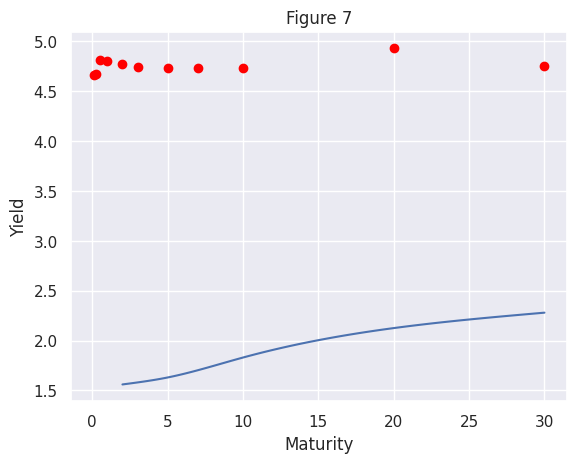
\includegraphics[width=0.8\textwidth]{gfx/m1l3_notes_fig7_cubic_spline_fit.png}
    \caption{Hình 7}
    \label{fig:m1l3_fig7}
\end{figure}

Hình 7 ở trên thể hiện đường cong lợi suất ước tính vào ngày 2020-01-10 bằng cách sử dụng phương pháp khớp spline bậc ba. Chúng ta có thể thấy với spline bậc ba, đường nối giữa hai điểm dữ liệu không phải là đường thẳng mà là đường cong. Với đường cong ước lượng này, chúng ta có thể tính toán lợi suất cho bất kỳ kỳ hạn nào nằm trên đường cong này nhằm mục đích định giá trái phiếu hoặc các phân tích lợi suất khác. Một khi chúng ta đã xây dựng được đường cong lợi suất này, chúng ta có thể dùng nó để lấy hệ số chiết khấu cho bất kỳ dòng tiền nào trong tương lai. Bằng cách tính tổng tất cả các dòng tiền trong tương lai đã chiết khấu từ một tài sản, chúng ta có thể có được giá trị hiện tại của tài sản đó và đánh giá xem liệu giá trị hiện tại đang định giá cao hay thấp hơn so với giá trị thực của tài sản.

\section[Kết luận]{Kết luận (Conclusion)}

Trong bài học này, đầu tiên chúng ta đã học xem lãi suất phi rủi ro là gì. Sau đó, chúng ta tính toán độ biến động của trái phiếu Kho bạc Hoa Kỳ tại các kỳ hạn khác nhau. Chúng ta cũng đã học hai phương pháp để khớp đường cong lợi suất bằng phương pháp Nelson Siegel và phương pháp spline bậc ba. Cuối cùng, chúng ta đã chứng minh cách triển khai hai phương pháp này để khớp đường cong lợi suất Trái phiếu Kho bạc Hoa Kỳ trong Python.

\section*{Tài liệu tham khảo (References)}

\begin{itemize}
    \item Pape. "Understanding the Nelson-Siegel-Svensson (NSS) Model for Bond Yield Curve Analysis." Medium, 2024 May 12. \url{https://medium.com/@pape14/understanding-the-nelson-siegel-svensson-nss-model-for-bond-yield-curve-analysis-2a23202cbf6b}.
    \item Svensson, Lars. "Estimating and Interpreting Forward Interest Rates: Sweden 1992-1994." NBER Working Paper Series, no. 4871, 1994.
\end{itemize}

Copyright 2024 WorldQuant University. This content is licensed solely for personal use. Redistribution or publication of this material is strictly prohibited.


\chapter{Đọc thêm 3: Nội suy Spline}
\label{ch:M1L3-reading}

\section{Phương pháp Nội suy Spline}

\subsection{Tại sao chúng ta cần Nội suy Spline?}

\subsubsection{Mục tiêu Học tập}
Sau khi hoàn thành thành công bài học này, bạn sẽ có khả năng:
1) giải thích tại sao nội suy bậc cao là một ý tưởng tồi,
2) cách nội suy spline có thể tránh được những cạm bẫy của nội suy bậc cao.

\subsubsection{Giới thiệu}
Nội suy đa thức liên quan đến việc tìm một đa thức bậc $n$ hoặc nhỏ hơn đi qua $n+1$ điểm. Một số phương pháp để thu được đa thức như vậy bao gồm phương pháp trực tiếp (còn gọi là phương pháp đa thức Vandermonde), phương pháp đa thức sai phân chia Newton, và phương pháp nội suy Lagrange.

Vậy phương pháp spline có phải là một phương pháp khác để thu được đa thức bậc $n$ này không? KHÔNG!
Thực tế, khi $n$ trở nên lớn, trong nhiều trường hợp, ta có thể gặp phải hành vi dao động trong đa thức nội suy. Hiện tượng này đã được Runge minh họa khi ông nội suy dữ liệu dựa trên một hàm đơn giản
\begin{equation}
y=\frac{1}{1+25x^{2}}
\end{equation}
trên một khoảng $[-1,1]$.

Ví dụ, lấy sáu điểm cách đều nhau trong $[-1,1]$ và tìm $y$ tại các điểm này từ Phương trình (5.5.1.1). Các giá trị này được cho trong Bảng 5.5.1.1.

\begin{table}[h]
\centering
\begin{tabular}{|c|c|}
\hline
$x$ & $y=\frac{1}{1+25x^{2}}$ \\
\hline
-1.0 & 0.038461 \\
-0.6 & 0.1 \\
-0.2 & 0.5 \\
0.2 & 0.5 \\
0.6 & 0.1 \\
1.0 & 0.038461 \\
\hline
\end{tabular}
\caption{Sáu điểm cách đều nhau trong $[-1,1]$.}
\end{table}

Bây giờ đi qua sáu điểm dữ liệu này, ta có thể xây dựng một đa thức nội suy bậc năm.
\begin{equation}
f_{5}(x)=1.2019x^{4}-1.7308x^{2}+0.56731 \quad -1\le x\le1
\end{equation}
Khi vẽ đồ thị đa thức bậc năm (Phương trình (5.5.1.2)) và hàm ban đầu (Phương trình (5.5.1.1)), như thấy ở Hình 5.5.1.1, bạn có thể thấy rằng chúng không khớp nhau tốt. Đa thức có đi qua sáu cặp dữ liệu của Bảng 5.5.1.1, nhưng nó thậm chí không đến gần hàm ban đầu tại nhiều điểm khác. Chỉ cần nhìn vào $x=0.85$, giá trị của hàm ban đầu là 0.052459, nhưng đa thức bậc năm cho bạn giá trị là -0.055762. Đó là một sai số thực tương đối khổng lồ lên tới 206.30\%.

\begin{figure}[htbp]
    \centering
    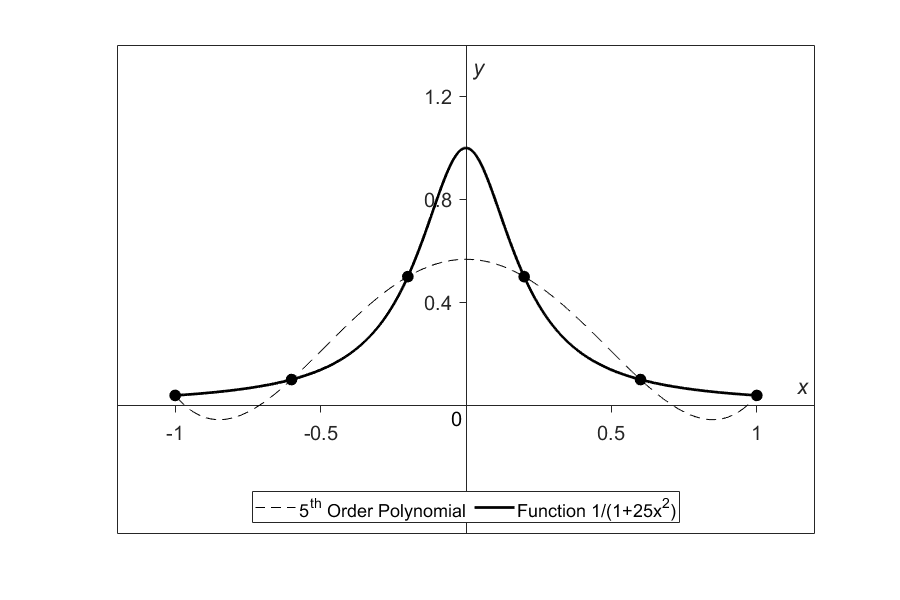
\includegraphics[width=0.8\textwidth]{gfx/m1l3_spline_runge_5th_order.png}
    \caption{Nội suy đa thức bậc năm với sáu điểm cách đều nhau.}
    \label{fig:spline_runge_5th_order}
\end{figure}

Người ta có thể nghĩ rằng việc chọn nhiều điểm hơn trong khoảng $[-1,1]$ sẽ cho chúng ta sự khớp tốt hơn giữa hàm ban đầu và hàm nội suy, nhưng nó thậm chí còn phân kỳ nhiều hơn (Hình 5.5.1.2). Ở đây, 20 điểm cách đều nhau đã được chọn trong khoảng $[-1,1]$ để vẽ một đa thức nội suy bậc 19. Tuy nhiên, nó đã làm tốt hơn việc xấp xỉ dữ liệu nhưng ngoại trừ gần các đầu mút nơi xấp xỉ tồi tệ hơn trước. Tại điểm đã chọn, $x=0.85$ giá trị của hàm ban đầu là 0.052459, trong khi ta nhận được -0.62944 từ đa thức bậc 19. Điều đó gây ra một sai số thực tương đối lớn tới 1299.9\%.

Trên thực tế, Runge phát hiện ra rằng khi bậc của đa thức tiến tới vô cùng, đa thức càng phân kỳ hơn trong khoảng $-1<x<-0.726$ và $0.726<x<1$.

\begin{figure}[htbp]
    \centering
    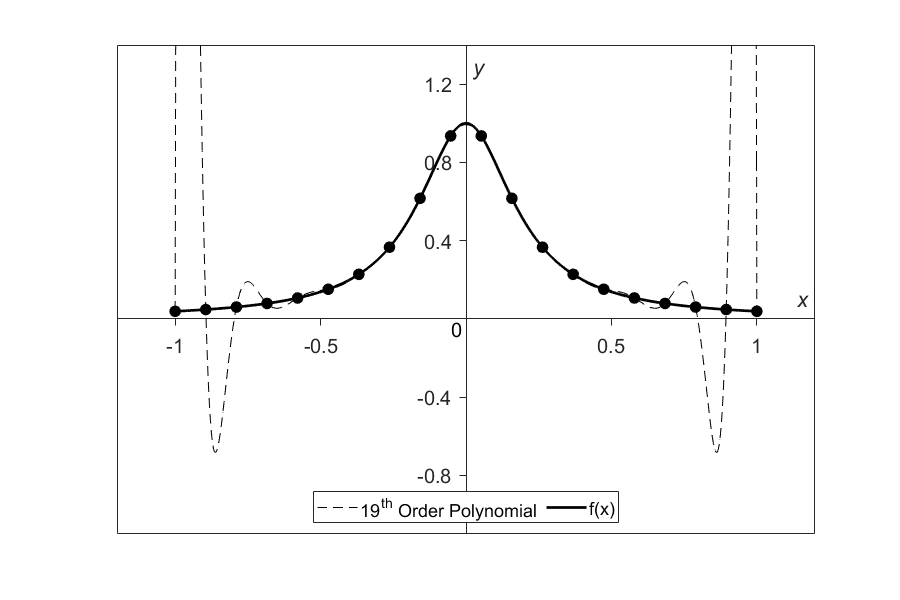
\includegraphics[width=0.8\textwidth]{gfx/m1l3_spline_runge_19th_order.png}
    \caption{Nội suy đa thức bậc mười chín với hai mươi điểm cách đều nhau.}
    \label{fig:spline_runge_19th_order}
\end{figure}

Vậy, giải pháp cho việc sử dụng thông tin từ nhiều điểm dữ liệu hơn, mà vẫn giữ cho hàm số tương đối trung thực với hành vi của dữ liệu là gì? Câu trả lời nằm ở nội suy spline và sẽ được thảo luận trong các bài học sau. Các loại nội suy spline phổ biến nhất được sử dụng là tuyến tính, bậc hai và bậc ba.

\subsection{Nội suy Spline Tuyến tính}

\subsubsection{Mục tiêu Học tập}
Sau khi hoàn thành thành công bài học này, bạn sẽ có khả năng:
1) phát triển hàm nội suy spline tuyến tính cho các điểm dữ liệu cho trước,
2) ước tính các điểm dữ liệu chưa biết từ hàm nội suy spline tuyến tính.

\subsubsection{Nội suy Spline Tuyến tính}
Cho $(x_{0},y_{0}),(x_{1},y_{1}),......,(x_{n-1},y_{n-1}),(x_{n},y_{n})$ , hãy tìm spline tuyến tính nội suy (Hình 5.5.2.1) cho dữ liệu. Quá trình này đơn giản chỉ liên quan đến việc vẽ các đường thẳng giữa các điểm liên tiếp.

\begin{figure}[htbp]
    \centering
    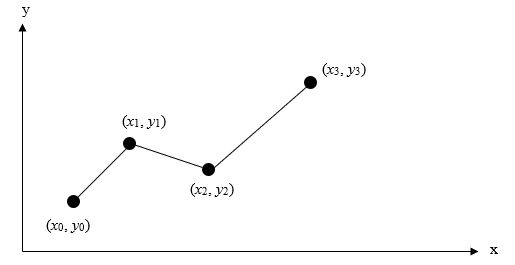
\includegraphics[width=0.8\textwidth]{gfx/m1l3_spline_piecewise_linear_points.png}
    \caption{Spline tuyến tính.}
    \label{fig:spline_piecewise_linear_points}
\end{figure}

Giả sử rằng dữ liệu trên được cho theo thứ tự tăng dần, spline tuyến tính nội suy, còn được gọi là spline bậc 1, $f(x)$ được cho bởi:
\begin{align}
f(x) &= f(x_0) + \frac{f(x_1)-f(x_0)}{x_1-x_0}(x-x_0), \quad x_0 \le x \le x_1 \\
&= f(x_1) + \frac{f(x_2)-f(x_1)}{x_2-x_1}(x-x_1), \quad x_1 \le x \le x_2 \\
&\vdots \nonumber \\
&= f(x_{n-1}) + \frac{f(x_n)-f(x_{n-1})}{x_n-x_{n-1}}(x-x_{n-1}), \quad x_{n-1} \le x \le x_n \label{eq:5.5.2.1}
\end{align}

Lưu ý rằng $y_{i}=f(x_{i})$ trong biểu thức trên và các số hạng của
\begin{equation}
\frac{f(x_{i})-f(x_{i-1})}{x_{i}-x_{i-1}}
\end{equation}
chỉ đơn giản là các độ dốc giữa $x_{i-1}$ và $x_i$.

\subsubsection{Ví dụ}
Vận tốc hướng lên của một tên lửa được cho như một hàm của thời gian trong Bảng 5.5.2.1 (Hình 5.5.2.2).

\begin{table}[h]
\centering
\begin{tabular}{|c|c|}
\hline
$t(s)$ & $v(t)$ $(m/s)$ \\
\hline
0 & 0 \\
10 & 227.04 \\
15 & 362.78 \\
20 & 517.35 \\
22.5 & 602.97 \\
30 & 901.67 \\
\hline
\end{tabular}
\caption{Vận tốc như một hàm của thời gian.}
\end{table}

Hãy xác định giá trị của vận tốc tại $t=16$ giây bằng cách sử dụng một spline tuyến tính nội suy.

\begin{figure}[htbp]
    \centering
    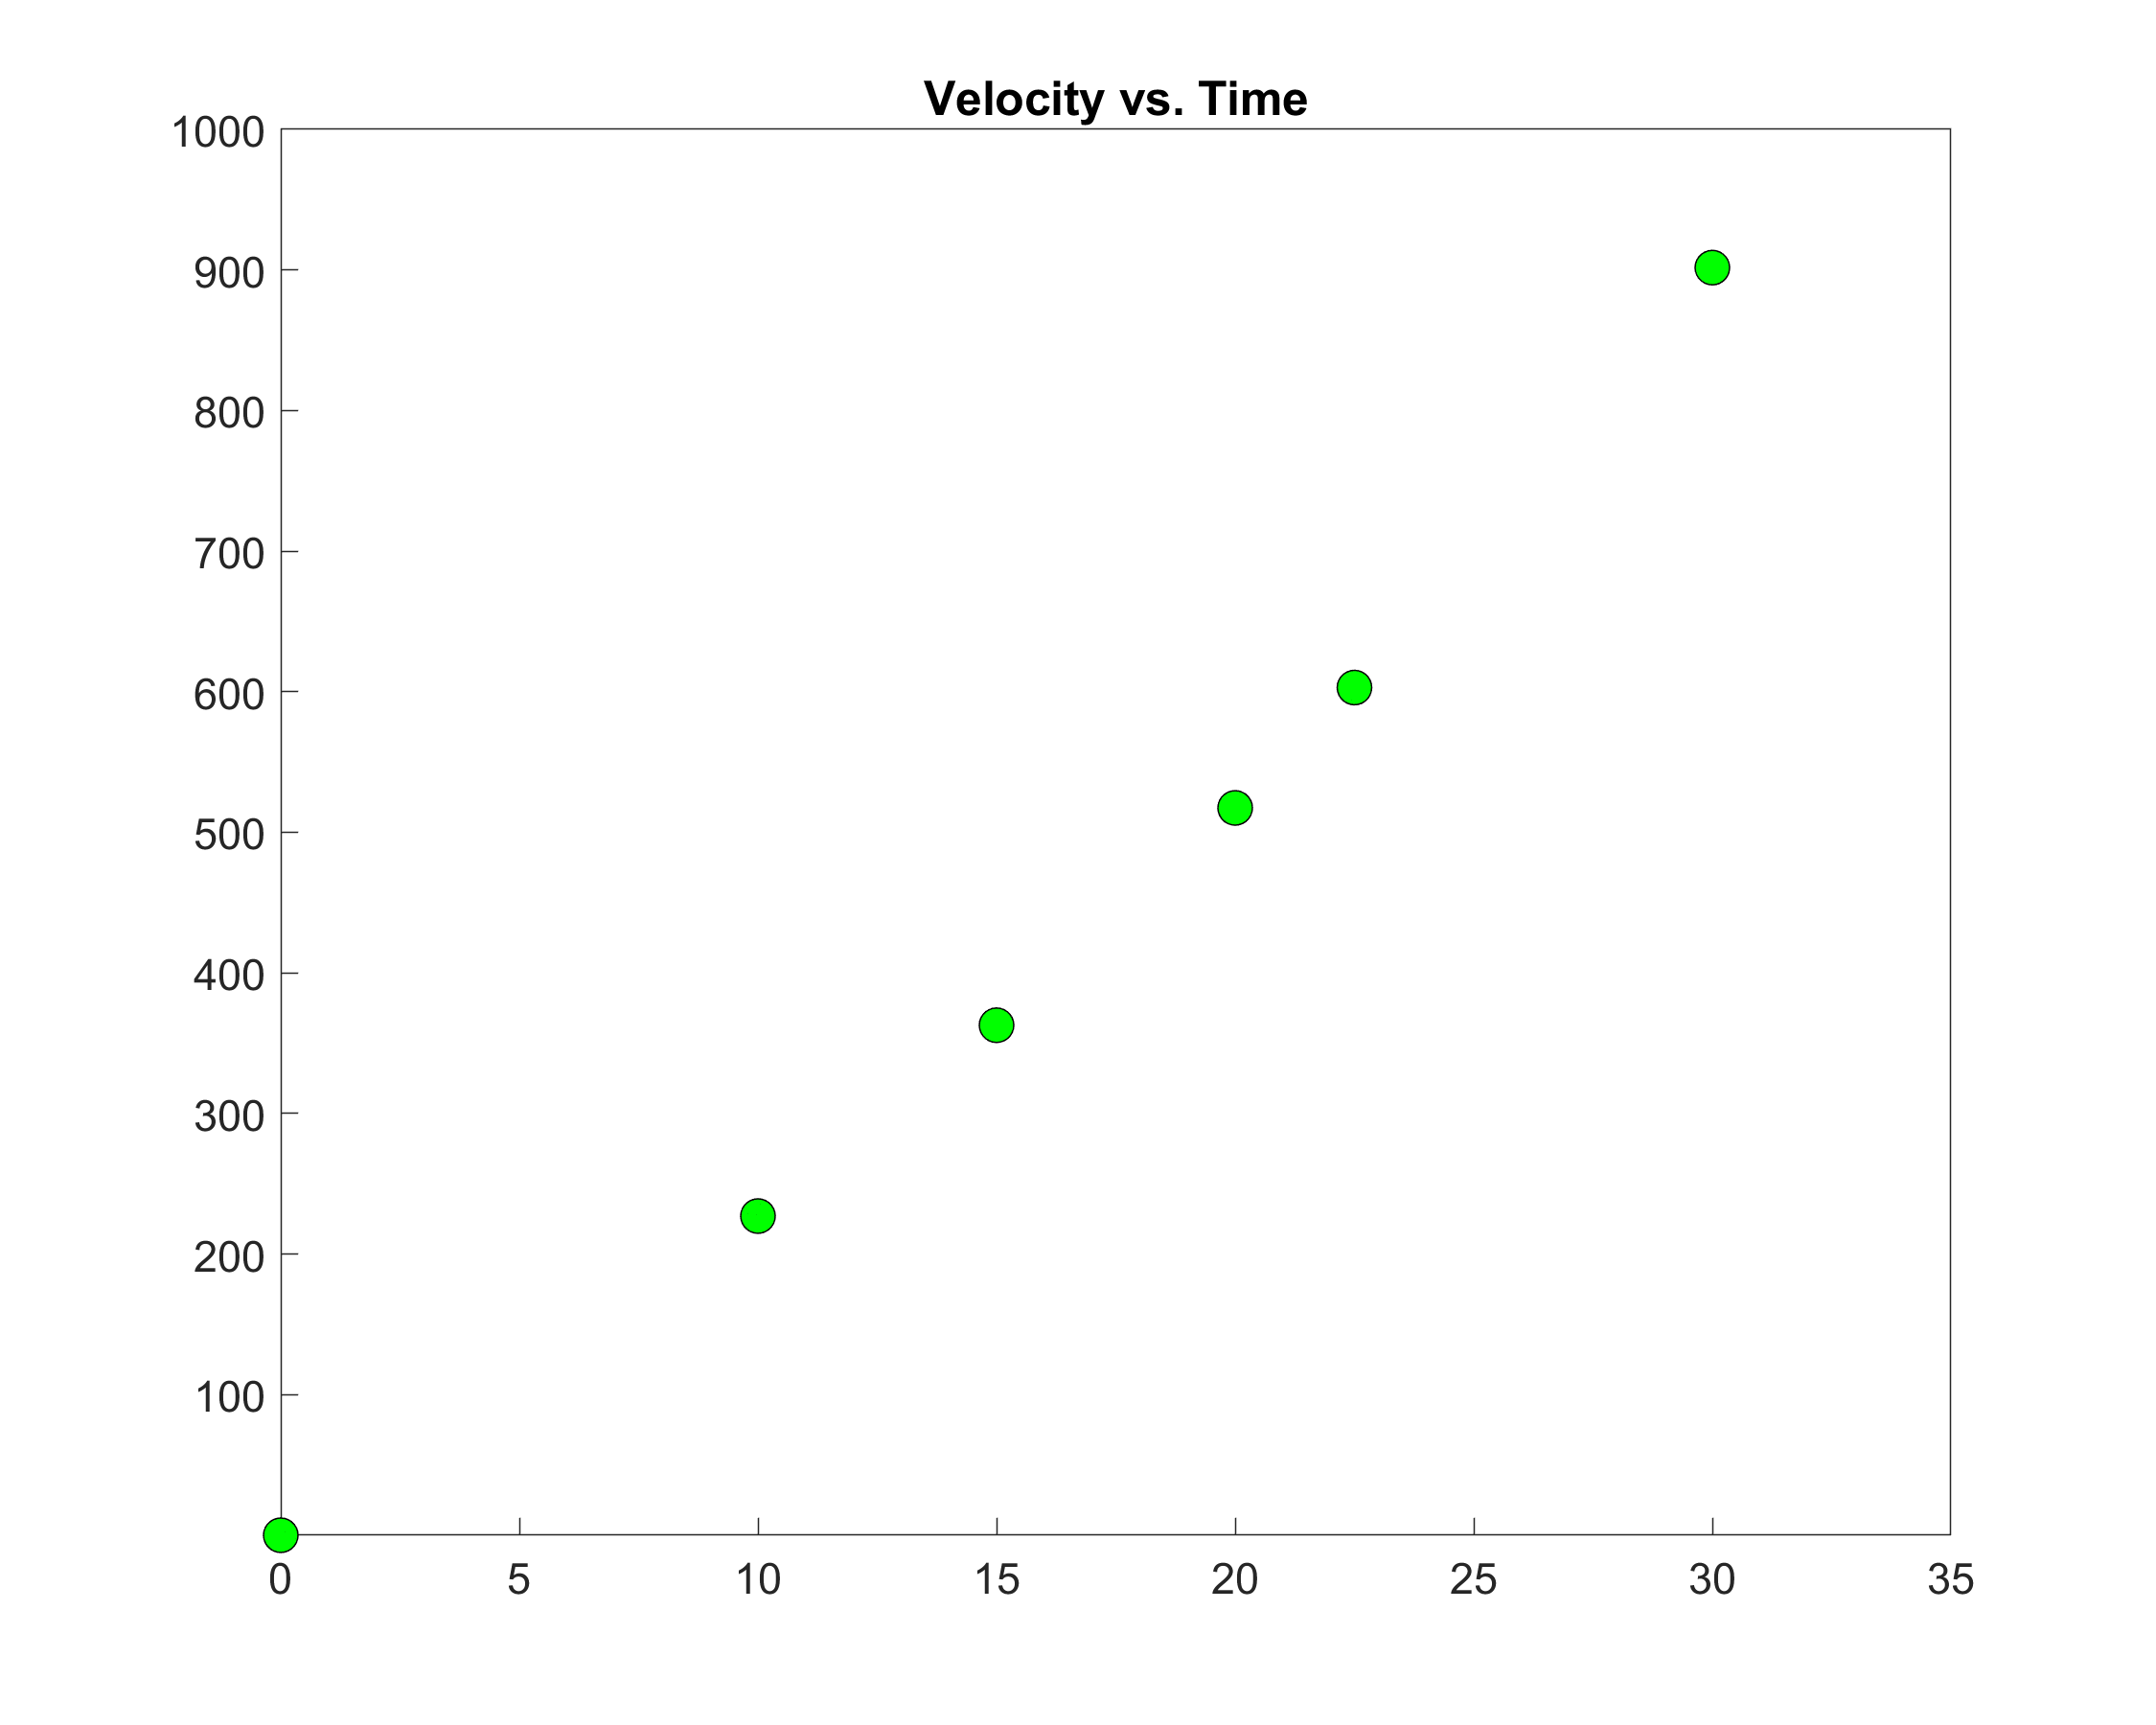
\includegraphics[width=0.8\textwidth]{gfx/m1l3_spline_velocity_vs_time.png}
    \caption{Đồ thị dữ liệu vận tốc theo thời gian cho ví dụ về tên lửa.}
    \label{fig:spline_velocity_vs_time}
\end{figure}

\textbf{Giải}

Vì chúng ta muốn tính vận tốc tại $t=16$ và sử dụng nội suy spline tuyến tính, chúng ta cần chọn hai điểm dữ liệu gần $t=16$ nhất đồng thời bao quanh $t=16$ để đánh giá nó. Hai điểm đó là $t_{0}=15$ và $t_{1}=20$

Khi đó
$t_{0}=15$, $v(t_{0})=362.78$ \\
$t_{1}=20$, $v(t_{1})=517.35$

mang lại
\begin{align*}
v(t) &= v(t_0) + \frac{v(t_1)-v(t_0)}{t_1-t_0}(t-t_0) \\
&= 362.78 + \frac{517.35-362.78}{20-15}(t-15) \\
&= 362.78 + 30.913(t-15) \quad 15 \le t \le 20
\end{align*}

Tại $t=16$,
\begin{align*}
v(16) &= 362.78 + 30.913(16-15) \\
&= 393.7~m/s
\end{align*}

Nội suy spline tuyến tính không khác gì nội suy đa thức tuyến tính. Nội suy spline tuyến tính vẫn chỉ sử dụng dữ liệu từ hai điểm dữ liệu liên tiếp, và dữ liệu từ các điểm khác hoàn toàn không được sử dụng. Ngoài ra, tại các điểm bên trong của dữ liệu, độ dốc của spline thay đổi đột ngột, điều này ngụ ý rằng đạo hàm bậc nhất "một cách giả tạo" không liên tục tại các điểm này. Vậy chúng ta vượt qua hai nhược điểm này như thế nào? Chúng ta có thể làm như vậy bằng cách sử dụng nội suy spline bậc hai hoặc bậc ba. Chúng ta sẽ thảo luận về các loại nội suy spline này trong các bài học sắp tới.

\subsection{Nội suy Spline Bậc hai}

\subsubsection{Mục tiêu Học tập}
Sau khi hoàn thành thành công bài học này, bạn sẽ có khả năng:
1) suy ra spline bậc hai nội suy cho dữ liệu rời rạc.

\subsubsection{Spline Bậc hai Nội suy}
Nội suy spline bậc hai là một phương pháp để khớp đường cong với dữ liệu. Đối với nội suy spline bậc hai, các hàm bậc hai từng phần xấp xỉ dữ liệu giữa hai điểm dữ liệu liên tiếp (Hình 5.5.3.1). Cho $(x_{0},y_{0}),(x_{1},y_{1}),.............,(x_{n-1},y_{n-1}),(x_{n},y_{n})$, khớp một spline bậc hai nội suy qua dữ liệu. Các hàm bậc hai của spline được cho bởi
\begin{align}
f(x) &= a_1x^2 + b_1x + c_1, \quad x_0 \le x \le x_1 \\
&= a_2x^2 + b_2x + c_2, \quad x_1 \le x \le x_2 \\
&\vdots \nonumber \\
&= a_nx^2 + b_nx + c_n, \quad x_{n-1} \le x \le x_n
\end{align}

Vậy làm thế nào để tìm các hệ số của các hàm bậc hai này? Có $3n$ hệ số như vậy:
$a_i, i=1,2,......,n$ \\
$b_i, i=1,2,.......,n$ \\
$c_i, i=1,2,.....,n$

Để tìm $3n$ ẩn số, người ta cần thiết lập $3n$ phương trình và sau đó giải đồng thời chúng. Các $3n$ phương trình này được tìm như sau.

\begin{figure}[htbp]
    \centering
    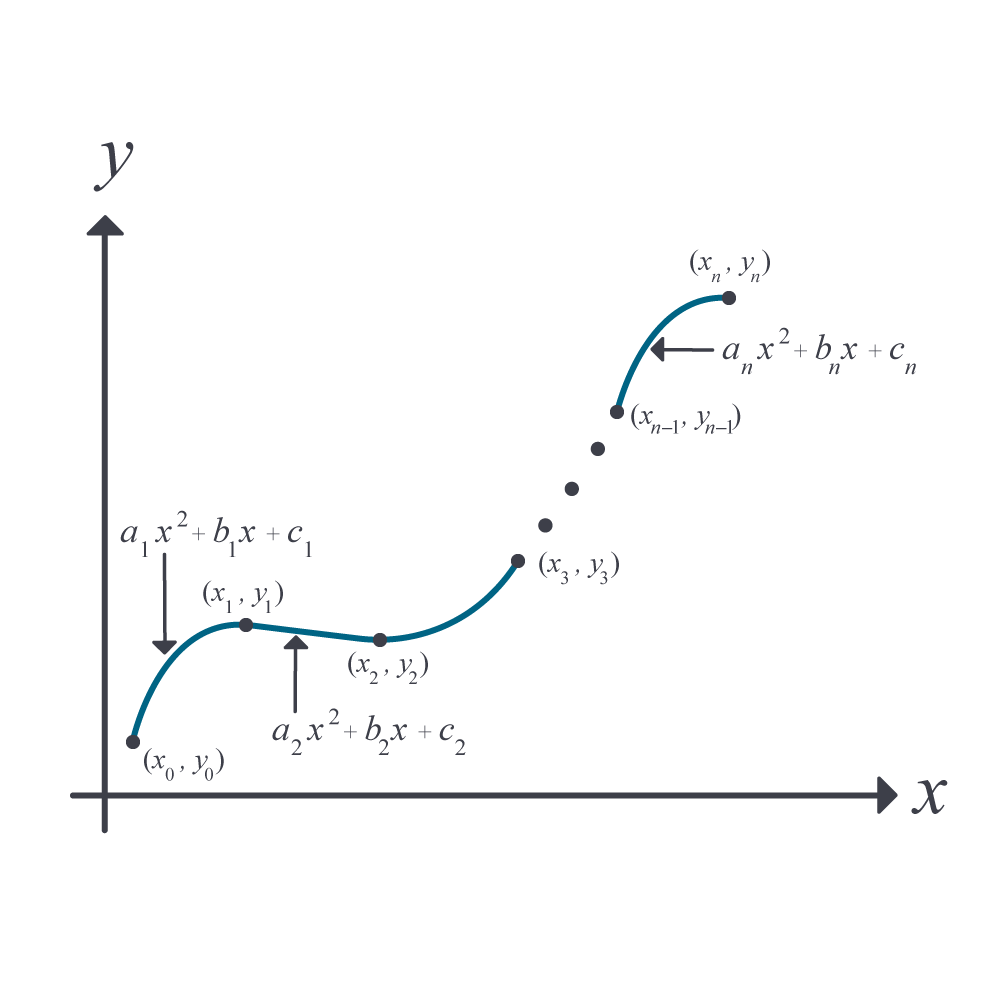
\includegraphics[width=0.8\textwidth]{gfx/m1l3_spline_quadratic_segments.png}
    \caption{Nội suy spline bậc hai}
    \label{fig:spline_quadratic_segments}
\end{figure}

1. Mỗi hàm bậc hai đi qua hai điểm dữ liệu liên tiếp:
\begin{align}
a_1{x_0}^2 + b_1x_0 + c_1 &= f(x_0) \nonumber \\
a_1{x_1}^2 + b_1x_1 + c_1 &= f(x_1) \nonumber \\
&\vdots \nonumber \\
a_i{x_{i-1}}^2 + b_ix_{i-1} + c_i &= f(x_{i-1}) \\
a_i{x_i}^2 + b_ix_i + c_i &= f(x_i) \nonumber \\
&\vdots \nonumber \\
a_n{x_{n-1}}^2 + b_nx_{n-1} + c_n &= f(x_{n-1}) \nonumber \\
a_n{x_n}^2 + b_nx_n + c_n &= f(x_n) \nonumber
\end{align}
Điều kiện này cho $2n$ phương trình vì có $n$ hàm bậc hai đi qua hai điểm dữ liệu liên tiếp.

2. Đạo hàm bậc nhất của hai hàm bậc hai liên tiếp là liên tục tại các điểm bên trong chung. Ví dụ, đạo hàm của hàm bậc hai thứ nhất $a_{1}x^{2}+b_{1}x+c_{1}$ là $2a_{1}x+b_{1}$. Đạo hàm của hàm bậc hai thứ hai $a_{2}x^{2}+b_{2}x+c_{2}$ là $2a_{2}x+b_{2}$, và hai giá trị này bằng nhau tại điểm bên trong chung $x=x_{1}$, mang lại:
$$2a_{1}x_{1}+b_{1}=2a_{2}x_{1}+b_{2}$$
$$2a_{1}x_{1}+b_{1}-2a_{2}x_{1}-b_{2}=0$$

Tương tự, tại các điểm bên trong khác $x_{2},...,x_{n-1}$
\begin{align}
2a_2x_2 + b_2 - 2a_3x_2 - b_3 &= 0 \nonumber \\
&\vdots \nonumber \\
2a_ix_i + b_i - 2a_{i+1}x_i - b_{i+1} &= 0 \\
&\vdots \nonumber \\
2a_{n-1}x_{n-1} + b_{n-1} - 2a_nx_{n-1} - b_n &= 0 \nonumber
\end{align}
Vì có $(n-1)$ điểm bên trong, chúng ta có $(n-1)$ phương trình như vậy.

3. Cho đến nay, tổng số phương trình thu được là $(2n)+(n-1)=(3n-1)$ phương trình. Vậy chúng ta vẫn cần thêm một phương trình nữa. Chúng ta có thể giả định hàm bậc hai đầu tiên là tuyến tính, tức là $a_{1}=0$. Một số người giả định hàm bậc hai cuối cùng là tuyến tính, tức là $a_{n}=0$.
Những người khác dựa trên cơ sở khoảng nào nhỏ hơn, $[x_{0},x_{1}]$ hoặc $[x_{n-1},x_{n}]$. Nếu $|x_{1}-x_{0}|\le|x_{n}-x_{n-1}|$, thì người ta sẽ chọn $a_{1}=0$; nếu không, chọn $a_{n}=0$.

Điều này cho chúng ta $3n$ phương trình tuyến tính đồng thời và $3n$ ẩn. Chúng có thể được giải bằng một số kỹ thuật dùng để giải hệ phương trình tuyến tính đồng thời tổng quát.

\subsection{Ứng dụng của Nội suy Spline Bậc hai}

\subsubsection{Mục tiêu Học tập}
Sau khi hoàn thành thành công bài học này, bạn sẽ có khả năng:
1) thực hiện nội suy spline bậc hai trên dữ liệu rời rạc,
2) đạo hàm một spline bậc hai nội suy khi cần thiết,
3) tích phân một spline bậc hai nội suy khi cần thiết.

\subsubsection{Các Ứng dụng}
Trong bài học trước, bạn đã tìm hiểu lý thuyết về phương pháp nội suy spline bậc hai. Trong bài học này, chúng tôi áp dụng lý thuyết để nội suy dữ liệu rời rạc cho trước thành một spline bậc hai nội suy.

\textbf{Ví dụ} \\
Vận tốc hướng lên của một tên lửa được cho như một hàm của thời gian là \\
Bảng 5.5.4.1. Vận tốc như một hàm của thời gian.

\begin{table}[h]
\centering
\begin{tabular}{|c|c|}
\hline
$t(s)$ & $v(t)$ $(m/s)$ \\
\hline
0 & 0 \\
10 & 227.04 \\
15 & 362.78 \\
20 & 517.35 \\
22.5 & 602.97 \\
30 & 901.67 \\
\hline
\end{tabular}
\end{table}

a) Xác định giá trị của vận tốc tại $t=16$ giây sử dụng nội suy spline bậc hai. \\
b) Sử dụng spline bậc hai nội suy, tìm quãng đường tên lửa đi được từ $t=11$ s đến $t=16$ s. \\
c) Sử dụng spline bậc hai nội suy, tìm gia tốc của tên lửa tại $t=16$ s.

\textbf{Giải} \\
a) Vì có sáu điểm dữ liệu, năm hàm bậc hai sẽ đi qua chúng.
\begin{align}
v(t) &= a_1t^2 + b_1t + c_1, \quad 0 \le t \le 10 \nonumber \\
&= a_2t^2 + b_2t + c_2, \quad 10 \le t \le 15 \nonumber \\
&= a_3t^2 + b_3t + c_3, \quad 15 \le t \le 20 \\
&= a_4t^2 + b_4t + c_4, \quad 20 \le t \le 22.5 \nonumber \\
&= a_5t^2 + b_5t + c_5, \quad 22.5 \le t \le 30 \nonumber
\end{align}

Các phương trình được tìm như sau. \\
1. Mỗi hàm bậc hai đi qua hai điểm dữ liệu liên tiếp. \\
Hàm bậc hai $a_{1}t^{2}+b_{1}t+c_{1}$ đi qua $t=0$ và $t=10$. \\
$a_{1}(0)^{2}+b_{1}(0)+c_{1}=0$ (5.5.4.E1.1) \\
$a_{1}(10)^{2}+b_{1}(10)+c_{1}=227.04$ (5.5.4.E1.2) \\
Hàm bậc hai $a_{2}t^{2}+b_{2}t+c_{2}$ đi qua $t=10$ và $t=15$. \\
$a_{2}(10)^{2}+b_{2}(10)+c_{2}=227.04$ (5.5.4.E1.3) \\
$a_{2}(15)^{2}+b_{2}(15)+c_{2}=362.78$ (5.5.4.E1.4) \\
Hàm bậc hai $a_{3}t^{2}+b_{3}t+c_{3}$ đi qua $t=15$ và $t=20$. \\
$a_{3}(15)^{2}+b_{3}(15)+c_{3}=362.78$ (5.5.4.E1.5) \\
$a_{3}(20)^{2}+b_{3}(20)+c_{3}=517.35$ (5.5.4.E1.6) \\
Hàm bậc hai $a_{4}t^{2}+b_{4}t+c_{4}$ đi qua $t=20$ và $t=22.5$. \\
$a_{4}(20)^{2}+b_{4}(20)+c_{4}=517.35$ (5.5.4.E1.7) \\
$a_{4}(22.5)^{2}+b_{4}(22.5)+c_{4}=602.97$ (5.5.4.E1.8) \\
Hàm bậc hai $a_{5}t^{2}+b_{5}t+c_{5}$ đi qua $t=22.5$ và $t=30$. \\
$a_{5}(22.5)^{2}+b_{5}(22.5)+c_{5}=602.97$ (5.5.4.E1.9) \\
$a_{5}(30)^{2}+b_{5}(30)+c_{5}=901.67$ (5.5.4.E1.10) 

2. Các hàm bậc hai có các đạo hàm liên tục tại các điểm dữ liệu bên trong chung. \\
Tại $t=10$: $2a_{1}(10)+b_{1}-2a_{2}(10)-b_{2}=0$ (5.5.4.E1.11) \\
Tại $t=15$: $2a_{2}(15)+b_{2}-2a_{3}(15)-b_{3}=0$ (5.5.4.E1.12) \\
Tại $t=20$: $2a_{3}(20)+b_{3}-2a_{4}(20)-b_{4}=0$ (5.5.4.E1.13) \\
Tại $t=22.5$: $2a_{4}(22.5)+b_{4}-2a_{5}(22.5)-b_{5}=0$ (5.5.4.E1.14)

3. Giả sử hàm bậc hai cuối cùng $a_{5}t^{2}+b_{5}t+c_{5}$ là tuyến tính (tại sao chúng ta chọn spline cuối cùng là tuyến tính thay vì cái đầu tiên?), \\
$a_{5}=0$ (5.5.4.E1.15)

Kết hợp các Phương trình từ (5.5.4.E1.1) đến (5.5.4.E1.15) dưới dạng ma trận ta được
\begin{align*}
\left[
\begin{array}{*{15}{c}}
0 & 0 & 1 & 0 & 0 & 0 & 0 & 0 & 0 & 0 & 0 & 0 & 0 & 0 & 0 \\
100 & 10 & 1 & 0 & 0 & 0 & 0 & 0 & 0 & 0 & 0 & 0 & 0 & 0 & 0 \\
0 & 0 & 0 & 100 & 10 & 1 & 0 & 0 & 0 & 0 & 0 & 0 & 0 & 0 & 0 \\
0 & 0 & 0 & 225 & 15 & 1 & 0 & 0 & 0 & 0 & 0 & 0 & 0 & 0 & 0 \\
0 & 0 & 0 & 0 & 0 & 0 & 225 & 15 & 1 & 0 & 0 & 0 & 0 & 0 & 0 \\
0 & 0 & 0 & 0 & 0 & 0 & 400 & 20 & 1 & 0 & 0 & 0 & 0 & 0 & 0 \\
0 & 0 & 0 & 0 & 0 & 0 & 0 & 0 & 0 & 400 & 20 & 1 & 0 & 0 & 0 \\
0 & 0 & 0 & 0 & 0 & 0 & 0 & 0 & 0 & 506.25 & 22.5 & 1 & 0 & 0 & 0 \\
0 & 0 & 0 & 0 & 0 & 0 & 0 & 0 & 0 & 0 & 0 & 0 & 506.25 & 22.5 & 1 \\
0 & 0 & 0 & 0 & 0 & 0 & 0 & 0 & 0 & 0 & 0 & 0 & 900 & 30 & 1 \\
20 & 1 & 0 & -20 & -1 & 0 & 0 & 0 & 0 & 0 & 0 & 0 & 0 & 0 & 0 \\
0 & 0 & 0 & 30 & 1 & 0 & -30 & -1 & 0 & 0 & 0 & 0 & 0 & 0 & 0 \\
0 & 0 & 0 & 0 & 0 & 0 & 40 & 1 & 0 & -40 & -1 & 0 & 0 & 0 & 0 \\
0 & 0 & 0 & 0 & 0 & 0 & 0 & 0 & 0 & 45 & 1 & 0 & -45 & -1 & 0 \\
0 & 0 & 0 & 0 & 0 & 0 & 0 & 0 & 0 & 0 & 0 & 0 & 1 & 0 & 0 
\end{array}
\right]
\begin{bmatrix}
a_1 \\ b_1 \\ c_1 \\ a_2 \\ b_2 \\ c_2 \\ a_3 \\ b_3 \\ c_3 \\ a_4 \\ b_4 \\ c_4 \\ a_5 \\ b_5 \\ c_5
\end{bmatrix}
=
\begin{bmatrix}
0 \\ 227.04 \\ 227.04 \\ 362.78 \\ 362.78 \\ 517.35 \\ 517.35 \\ 602.97 \\ 602.97 \\ 901.67 \\ 0 \\ 0 \\ 0 \\ 0 \\ 0
\end{bmatrix}
\end{align*}

Giải 15 phương trình tuyến tính đồng thời trên cho 15 ẩn số ta được
\begin{table}[h]
\centering
\begin{tabular}{|c|c|c|c|}
\hline
$i$ & $a_i$ & $b_i$ & $c_i$ \\
\hline
1 & -0.15667 & 24.271 & 0 \\
2 & 1.2021 & -2.9053 & 135.88 \\
3 & -0.44893 & 46.627 & -235.61 \\
4 & 2.2315 & -60.589 & 836.55 \\
5 & 0 & 39.827 & -293.13 \\
\hline
\end{tabular}
\end{table}

Do đó, spline bậc hai nội suy được cho bởi
\begin{align}
v(t) &= -0.15667t^2 + 24.271t, \quad 0 \le t \le 10 \nonumber \\
&= 1.2021t^2 - 2.9053t + 135.88, \quad 10 \le t \le 15 \nonumber \\
&= -0.44893t^2 + 46.627t - 235.61, \quad 15 \le t \le 20 \\
&= 2.2315t^2 - 60.589t + 836.55, \quad 20 \le t \le 22.5 \nonumber \\
&= 39.827t - 293.13, \quad 22.5 \le t \le 30 \nonumber
\end{align}

Tại $t=16~s$
\begin{align}
v(16) &= -0.44893(16)^2 + 46.627(16) - 235.61 \nonumber \\
&= 395.50~m/s
\end{align}

b) Quãng đường tên lửa đi được từ 11 s đến 16 s giây có thể được tính như sau
\begin{equation}
s(16)-s(11)=\int_{11}^{16}v(t)dt
\end{equation}

Nhưng vì có vài hàm bậc hai có hiệu lực qua các cận tích phân, chúng ta cần chia tích phân một cách tương ứng. Sử dụng Phương trình (5.5.4.E1.16).
\begin{align}
v(t) &= 1.2021t^2 - 2.9053t + 135.88, \quad 10 \le t \le 15 \nonumber \\
&= -0.44893t^2 + 46.627t - 235.61, \quad 15 \le t \le 20
\end{align}

Sau đó
\begin{align}
s(16)-s(11) &= \int_{11}^{16}v(t)dt \nonumber \\
&= \int_{11}^{15}v(t)dt+\int_{15}^{16}v(t)dt
\end{align}

Thay thế các hàm bậc hai thích hợp mang lại
\begin{align}
s(16)-s(11) &= \int_{11}^{15} (1.2021t^2 - 2.9053t + 135.88) dt \nonumber \\
&\quad + \int_{15}^{16} (-0.44893t^2 + 46.627t - 235.61) dt \nonumber \\
&= \left[1.2021\frac{t^3}{3} - 2.9053\frac{t^2}{2} + 135.88t\right]_{11}^{15} \\
&\quad + \left[-0.44893\frac{t^3}{3} + 46.627\frac{t^2}{2} - 235.61t\right]_{15}^{16} \nonumber \\
&= 1211.49 + 379.22 \nonumber \\
&= 1590.7~m \nonumber
\end{align}

c) Gia tốc tại $t=16~s$ là bao nhiêu?
\begin{equation}
a(16)=\frac{dv}{dt}\bigg|_{t=16}
\end{equation}

Ở đây chúng ta sử dụng hàm bậc hai thứ ba từ Phương trình (5.5.4.E1.15),
$$ -0.44893t^{2}+46.627t-235.61, \quad 15\le t\le20 $$
vì $t=16$ nằm trong miền của $15\le t\le20$.

Vậy
\begin{align}
a(t) &= \frac{d}{dt}v(t) \nonumber \\
&= \frac{d}{dt}(-0.44893t^2 + 46.627t - 235.61) \nonumber \\
&= -0.89786t + 46.627, \quad 15 \le t \le 20
\end{align}

\begin{align}
a(16) &= -0.89786(16) + 46.627 \nonumber \\
&= 32.261~m/s^2
\end{align}


\subsection{Phác thảo Nội suy Spline Bậc ba}

\subsubsection{Mục tiêu Học tập}
Sau khi hoàn thành thành công bài học này, bạn sẽ có khả năng:
1) phác thảo phép suy luận của nội suy spline bậc ba.

\subsubsection{Giới thiệu}
Giống như nội suy spline bậc hai, nội suy spline bậc ba là một phương pháp để khớp đường cong với dữ liệu. Nội suy spline bậc ba là bậc spline phổ biến nhất được sử dụng.

\subsubsection{Spline Bậc ba Nội suy}
Cho $n+1$ điểm dữ liệu, $(x_{0},y_{0}),$ $(x_{1},y_{1}),...,(x_{n},y_{n})$ hãy khớp một spline bậc ba nội suy qua dữ liệu. Đối với nội suy spline bậc ba, các đa thức bậc ba từng phần xấp xỉ dữ liệu giữa hai điểm liên tiếp. Spline bậc ba nội suy được cho bởi các đa thức bậc ba như
\begin{align}
f(x) &= a_1x^3 + b_1x^2 + c_1x + d_1, \quad x_0 \le x \le x_1 \nonumber \\
&= a_2x^3 + b_2x^2 + c_2x + d_2, \quad x_1 \le x \le x_2 \\
&\vdots \nonumber \\
&= a_nx^3 + b_nx^2 + c_nx + d_n, \quad x_{n-1} \le x \le x_n \nonumber
\end{align}

Vậy, làm thế nào để tìm các hệ số của những đa thức bậc ba này? Có $4n$ hệ số như vậy được đưa ra dưới đây.
\begin{align}
a_i, \quad & i=1,2,...,n \nonumber \\
b_i, \quad & \nonumber \\
c_i, \quad & \nonumber \\
d_i, \quad & i=1,2,...,n
\end{align}

Để tìm $4n$ ẩn số, chúng ta cần thiết lập $4n$ phương trình tuyến tính đồng thời. Khái quát việc thiết lập các phương trình này như sau.
Chúng ta có $n+1$ điểm dữ liệu. Trong số $n+1$ điểm này, hai là các điểm dữ liệu bên ngoài (đầu mút), trong khi có $(n+1)-2=n-1$ điểm dữ liệu bên trong.

1. Mỗi hàm bậc ba phải đi qua hai điểm liên tiếp. Vì chúng ta có $n$ spline, chúng ta sẽ nhận được $2n$ phương trình.
2. Đạo hàm bậc nhất của hai hàm bậc ba liên tiếp là liên tục tại điểm dữ liệu bên trong chung. Vì chúng ta có $(n-1)$ điểm bên trong, chúng ta sẽ nhận được $2(n-1)$ phương trình.
3. Đạo hàm bậc hai của hai hàm bậc ba liên tiếp là liên tục tại điểm dữ liệu bên trong chung. Vì chúng ta có $(n-1)$ điểm bên trong, chúng ta sẽ nhận được $2(n-1)$ phương trình.

Cho đến nay, chúng ta đã phác thảo rằng có thể thiết lập
\begin{equation}
(2n)+(n-1)+(n-1) = 4n-2
\end{equation}
phương trình. Chúng ta cần hai phương trình nữa, và một số loại điều kiện có thể được sử dụng để lấy chúng. Một vài điều kiện phổ biến được sử dụng như sau.
1. Giả sử rằng các spline bậc ba đầu tiên và cuối cùng là các hàm bậc hai $a_{1}=0$ và $a_{n}=0$ để nhận hai phương trình bổ sung. Giả định này được gọi là điều kiện biên bậc hai.
2. Giả sử đạo hàm bậc hai của spline bậc ba đầu tiên và cuối cùng là bằng không $(6a_{1}x_{0}+2b_{1}=0$ và $6a_{n}x_{n}+2b_{n}=0)$ tại các điểm bên ngoài tương ứng để nhận hai phương trình bổ sung. Giả định này được gọi là điều kiện biên tự nhiên.

\subsection{Bài kiểm tra Trắc nghiệm}

(1). $n$ điểm dữ liệu sau đây, $(x_{1},y_{1})$, $(x_{2},y_{2}),........(x_{n},y_{n})$, được cho. Để tiến hành nội suy spline bậc hai, dữ liệu x cần được
(A) cách đều nhau
(B) đặt theo thứ tự tăng dần hoặc giảm dần của các giá trị x
(C) số nguyên
(D) số dương

(2). Trong nội suy spline bậc ba,
(A) các đạo hàm bậc nhất của hàm bậc ba là liên tục tại các điểm dữ liệu bên trong
(B) các đạo hàm bậc hai của hàm bậc ba là liên tục tại các điểm dữ liệu bên trong
(C) các đạo hàm bậc nhất và bậc hai của hàm bậc ba là liên tục tại các điểm dữ liệu bên trong
(D) các đạo hàm bậc ba của hàm bậc ba là liên tục tại các điểm dữ liệu bên trong

(3). Dữ liệu y theo x chưa hoàn chỉnh sau đây được cho.
\begin{table}[h]
\centering
\begin{tabular}{|c|c|c|c|c|c|c|}
\hline
$x$ & 1 & 2 & 4 & 6 & 7 \\
\hline
$y$ & 5 & 11 & ???? & ???? & 32 \\
\hline
\end{tabular}
\end{table}

Dữ liệu được khớp bởi các spline bậc hai nội suy cho bởi
\begin{align}
f(x) &= ax-1, \quad 1 \le x \le 2 \nonumber \\
&= -2x^2+14x-9, \quad 2 \le x \le 4 \nonumber \\
&= bx^2+cx+d, \quad 4 \le x \le 6 \nonumber \\
&= 25x^2-303x+928, \quad 6 \le x \le 7
\end{align}
với a, b, c, và d là các hằng số. Giá trị của c gần nhất với
(A) -303.00
(B) -144.50
(C) 0.0000
(D) 14.000

(4). Dữ liệu y theo x chưa hoàn chỉnh sau đây được cho.
\begin{table}[h]
\centering
\begin{tabular}{|c|c|c|c|c|c|c|}
\hline
$x$ & 1 & 2 & 4 & 6 & 7 \\
\hline
$y$ & 5 & 11 & ???? & ???? & 32 \\
\hline
\end{tabular}
\end{table}

Dữ liệu được khớp bởi spline bậc hai nội suy cho bởi
\begin{align}
f(x) &= ax-1, \quad 1 \le x \le 2 \nonumber \\
&= -2x^2+14x-9, \quad 2 \le x \le 4 \nonumber \\
&= bx^2+cx+d, \quad 4 \le x \le 6 \nonumber \\
&= ex^2+fx+g, \quad 6 \le x \le 7
\end{align}
với a, b, c, d, e, f, và g là các hằng số. Giá trị của $\frac{df}{dx}$ tại $x=2.6$ gần nhất với
(A) -144.50
(B) -4.0000
(C) 3.6000
(D) 12.200

(5). Dữ liệu y theo x chưa hoàn chỉnh sau đây được cho.
\begin{table}[h]
\centering
\begin{tabular}{|c|c|c|c|c|c|c|}
\hline
$x$ & 1 & 2 & 4 & 6 & 7 \\
\hline
$y$ & 5 & 11 & ???? & ???? & 32 \\
\hline
\end{tabular}
\end{table}

Dữ liệu được khớp bởi spline bậc hai nội suy cho bởi
\begin{align}
f(x) &= ax-1, \quad 1 \le x \le 2, \nonumber \\
&= -2x^2+14x-9, \quad 2 \le x \le 4 \nonumber \\
&= bx^2+cx+d, \quad 4 \le x \le 6 \nonumber \\
&= 25x^2-303x+928, \quad 6 \le x \le 7
\end{align}
với a, b, c, và d là các hằng số. Giá trị ước tính của $\int_{1.5}^{3.5}f(x)dx$ là bao nhiêu?
(A) 23.500
(B) 25.667
(C) 25.750
(D) 28.000

(6). Một robot cần đi theo một con đường lần lượt đi qua sáu điểm như hình vẽ. Để tìm đường đi ngắn nhất mà cũng nhẵn, bạn sẽ đề xuất phương án nào sau đây?

\begin{figure}[htbp]
    \centering
    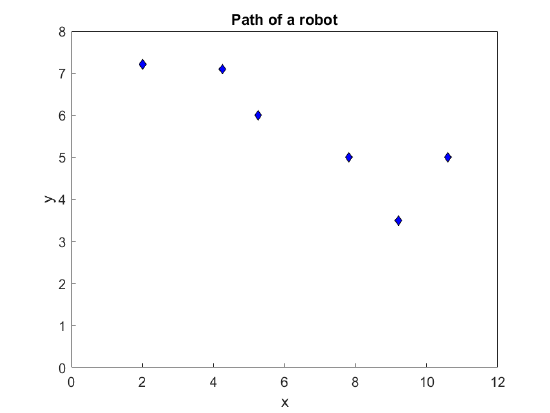
\includegraphics[width=0.8\textwidth]{gfx/m1l3_spline_path_of_robot.png}
    \caption{Đường đi của một con robot}
    \label{fig:spline_path_of_robot}
\end{figure}

(A) Cho một đa thức bậc năm đi qua dữ liệu
(B) Cho spline tuyến tính nội suy đi qua dữ liệu
(C) Cho spline bậc hai nội suy đi qua dữ liệu
(D) Hồi quy dữ liệu thành một đa thức bậc hai

\subsection{Bài tập}

(1). Dữ liệu y theo x sau đây được cho.
\begin{table}[h]
\centering
\begin{tabular}{|c|c|c|c|}
\hline
$x$ & 2 & 3 & 6 \\
\hline
$y$ & 4.75 & 5.25 & 45 \\
\hline
\end{tabular}
\end{table}

a) Thiết lập các phương trình để giải tìm spline bậc hai nội suy đi qua dữ liệu.
b) Sử dụng một chương trình như MATLAB để giải các phương trình và sau đó viết ra spline bậc hai nội suy.
c) Ước tính giá trị của $y(3.6)$.

\textbf{Trả lời} \\
a)
\begin{align*}
\begin{bmatrix}
4 & 2 & 1 & 0 & 0 & 0 \\
9 & 3 & 1 & 0 & 0 & 0 \\
0 & 0 & 0 & 9 & 3 & 1 \\
0 & 0 & 0 & 36 & 6 & 1 \\
6 & 1 & 0 & -6 & -1 & 0 \\
1 & 0 & 0 & 0 & 0 & 0
\end{bmatrix}
\begin{bmatrix}
a_1 \\ b_1 \\ c_1 \\ a_2 \\ b_2 \\ c_2
\end{bmatrix}
=
\begin{bmatrix}
4.75 \\ 5.25 \\ 5.25 \\ 45 \\ 0 \\ 0
\end{bmatrix}
\end{align*}

b)
\begin{table}[h]
\centering
\begin{tabular}{|c|c|c|c|}
\hline
$i$ & $a_i$ & $b_i$ & $c_i$ \\
\hline
1 & 0 & 0.5 & 3.75 \\
2 & 4.25 & -25 & 42 \\
\hline
\end{tabular}
\end{table}

c) 7.08

(2). Dữ liệu y theo x sau đây được cho.
\begin{table}[h]
\centering
\begin{tabular}{|c|c|c|c|c|c|}
\hline
$x$ & 1 & 2 & 3 & 5 & 6 \\
\hline
$y$ & 4.75 & 4 & 5.25 & 15 & 45 \\
\hline
\end{tabular}
\end{table}

Dữ liệu được khớp bởi spline bậc hai nội suy cho bởi
\begin{align}
f(x) &= -0.75x+5.5, \quad 1 \le x \le 2 \nonumber \\
&= 2x^2-8.75x+13.5, \quad 2 \le x \le 3 \nonumber \\
&= cx^2+gx+h, \quad 3 \le x \le 5 \nonumber \\
&= jx^2+kx+l, \quad 5 \le x \le 6
\end{align}
với c, g, h, j, k, và l là các hằng số.

a) Tìm giá trị của c, g, h, j, k, và l.
b) So sánh giá trị của hàm tại $x=2.3$ sử dụng spline tuyến tính nội suy và spline bậc hai nội suy.

\textbf{Trả lời} \\
a) $c=0.8125$ \\
$g=-1.625$ \\
$h=2.8125$ \\
$j=23.5$ \\
$k=-228.5$ \\
$l=570$

b) tuyến tính $= 4.375$; bậc hai $= 3.955$

(3). Dữ liệu y theo x chưa hoàn chỉnh sau đây được cho.
\begin{table}[h]
\centering
\begin{tabular}{|c|c|c|c|c|c|c|}
\hline
$x$ & 1 & 2.2 & 3.7 & 5.1 & 6 \\
\hline
$y$ & 4.25 & 6 & 5.25 & 15.1 & ????? \\
\hline
\end{tabular}
\end{table}

Dữ liệu được khớp bởi spline bậc hai nội suy cho bởi
\begin{align}
f(x) &= 1.4583x+2.7917, \quad 1 \le x \le 2.2 \nonumber \\
&= -1.3056x^2+7.2028x-3.5278, \quad 2.2 \le x \le 3.7 \nonumber \\
&= cx^2+gx+h, \quad 3.7 \le x \le 5.1 \nonumber \\
&= jx^2+kx+l, \quad 5.1 \le x \le 6
\end{align}
với c, g, h, j, k, và l là các hằng số. Giá trị của g là bao nhiêu? Hãy trình bày tất cả các bước của bạn một cách rõ ràng.

\textbf{Trả lời} \\
$g=-52.6391$

(4). Dữ liệu y theo x chưa hoàn chỉnh sau đây được cho.
\begin{table}[h]
\centering
\begin{tabular}{|c|c|c|c|c|c|c|}
\hline
$x$ & 1 & 2.2 & 3.7 & 5.1 & 6 \\
\hline
$y$ & 4.25 & 6 & 5.25 & ???? & ????? \\
\hline
\end{tabular}
\end{table}

Dữ liệu được khớp bởi spline bậc hai nội suy cho bởi
\begin{align}
f(x) &= 1.4583x+2.7917, \quad 1 < x < 2.2 \nonumber \\
&= -1.3056x^2+7.2028x-3.5272, \quad 2.2 \le x \le 3.7 \nonumber \\
&= cx^2+gx+h, \quad 3.7 \le x \le 5.1 \nonumber \\
&= jx^2+kx+l, \quad 5.1 \le x \le 6
\end{align}
với c, g, h, j, k, và l là các hằng số. Giá trị của $\frac{df}{dx}$ tại $x=2.67$ là bao nhiêu?

\textbf{Trả lời} \\
0.23133

(5). Dữ liệu y theo x chưa hoàn chỉnh sau đây được cho.
\begin{table}[h]
\centering
\begin{tabular}{|c|c|c|c|c|c|c|}
\hline
$x$ & 1 & 2.2 & 3.7 & 5.1 & 6 \\
\hline
$y$ & 4.25 & 6 & 5.25 & ???? & ????? \\
\hline
\end{tabular}
\end{table}

Dữ liệu được khớp bởi spline bậc hai nội suy cho bởi
\begin{align}
f(x) &= 1.4583x+2.7917, \quad 1 \le x \le 2.2 \nonumber \\
&= -1.3056x^2+7.2028x-3.5272, \quad 2.2 \le x \le 3.7 \nonumber \\
&= cx^2+gx+h, \quad 3.7 \le x \le 5.1 \nonumber \\
&= jx^2+kx+l, \quad 5.1 \le x \le 6
\end{align}
với c, g, h, j, k, và l là các hằng số. Giá trị của $\int_{1.5}^{2.5}f(x)dx$ là bao nhiêu?

\textbf{Trả lời} \\
5.6965

(6). Cho ba điểm dữ liệu (1,6), (3, 28), và (10, 231), người ta nhận thấy rằng hàm số $y=2x^2+3x+1$ đi qua ba điểm dữ liệu này. Để tìm chiều dài của đường cong đa thức từ $x=5$ đến $x=8$, một sinh viên sử dụng công thức $S=\int_{a}^{b}\sqrt{1+(dy/dx)^2}dx$. Tuy nhiên, công thức này cho sinh viên một tích phân không thể giải chính xác được. Thay vào đó, sinh viên này xấp xỉ đường cong đa thức bằng cách vẽ spline tuyến tính nội suy bao gồm các hàm từng phần từ $x=5$ đến $x=6$, từ $x=6$ đến $x=7$ và từ $x=7$ đến $x=8$. Sinh viên sau đó tìm chiều dài của spline tuyến tính nội suy từ $x=5$ đến $x=8$. Ước tính của sinh viên về chiều dài của hàm số từ $x=5$ đến $x=8$ là bao nhiêu?

\textbf{Trả lời} \\
87.052 (nhận được 87 làm câu trả lời là sai)



% ---- Lesson 4: Government Bond Yield Bivariate Analysis and Yield Curve Analysis ----
% Thứ tự đọc: Lesson Notes (trong VM, xem ghi chú trong chương) -> Đọc thêm
\chapter{Phân tích Biến đôi và Phân tích Đường cong Lợi suất}
\label{ch:M1L4}

\section*{Lesson Notes}

\textbf{Dự án} \\
\textbf{Thời gian đọc:} 60 phút \\
\textbf{Kiến thức nền tảng:} Trái phiếu Kho bạc Hoa Kỳ (U.S. Treasury Bonds), Đường cong lợi suất (Yield Curve), Đại số tuyến tính (Linear Algebra), Python cơ bản \\
\textbf{Từ khóa:} Đường cong giá-lợi suất trái phiếu (Bond price-yield curve), Lãi suất phi rủi ro (Risk free interest rate), Nelson Siegel, Spline bậc ba (Cubic Spline)

Trong bài học trước, chúng ta đã giới thiệu về đường cong giá - lợi suất Trái phiếu Kho bạc Hoa Kỳ và thảo luận về hình dáng của đường cong này. Chúng ta cũng đã tìm hiểu các phương pháp để khớp đường cong Kho bạc Hoa Kỳ bằng cách sử dụng các kỹ thuật khớp đa thức. Trong bài học này, chúng ta sẽ tiếp tục học các phương pháp phân tích mới để hiểu rõ hơn về lợi suất Trái phiếu Kho bạc Hoa Kỳ. Đầu tiên, chúng ta sẽ khám phá các mối quan hệ biến đôi (bivariate relationships) của các mức lợi suất khác nhau, bao gồm tương quan (correlation) và hiệp phương sai (covariance). Sau đó, chúng ta sẽ học một kỹ thuật mới để trích xuất các đặc điểm chính của đường cong lợi suất Kho bạc Hoa Kỳ nhằm phân tích hành vi của đường cong này.

\section[Phân tích Biến đôi]{Phân tích Biến đôi (Bivariate Analysis)}

Phân tích biến đôi là một tập hợp các phương pháp nhằm phân tích mối quan hệ giữa hai biến số. Trong tài chính, chúng ta đặc biệt quan tâm đến việc hiểu cách hai biến số tương tác với nhau. Trong bài học này, chúng ta sẽ xem xét lợi suất của các Trái phiếu Kho bạc Hoa Kỳ khác nhau và cách chúng dịch chuyển trong mối tương quan lẫn nhau. Công cụ phân tích biến đôi đầu tiên chúng ta sẽ học là hiệp phương sai (covariance).

\subsection[Hiệp phương sai]{Hiệp phương sai (Covariance)}

Hiệp phương sai là một thước đo để đánh giá mức độ dịch chuyển cùng nhau của hai biến số. Cụ thể, hiệp phương sai tính toán độ lớn của biến động mà hai biến số thể hiện. Dưới đây là công thức tính hiệp phương sai:

$$Cov(X,Y)=E[(X-E[X])(Y-E[Y])]$$

Dưới đây là một số tính chất của hiệp phương sai:
1. Nếu hiệp phương sai mang dấu dương, điều đó có nghĩa là hai biến số dịch chuyển cùng chiều.
2. Nếu hiệp phương sai mang dấu âm, hai biến số dịch chuyển ngược chiều nhau.
3. Nếu hiệp phương sai bằng 0, hai biến số không có tương quan tuyến tính (uncorrelated).

Giá trị tuyệt đối của hiệp phương sai giữa hai biến số càng cao, mối quan hệ (dương hoặc âm) giữa hai biến số càng mạnh. Hãy cùng trích xuất một số dữ liệu lợi suất Trái phiếu Kho bạc Hoa Kỳ để minh họa cho hiệp phương sai giữa hai mức lợi suất khác nhau.

Ma trận hiệp phương sai là một thước đo phân tích biến đôi cho hai biến số. Tuy nhiên, khi chúng ta có một số lượng biến lớn hơn và muốn biết mối quan hệ theo cặp của các biến này, chúng ta sẽ cần đến một ma trận hiệp phương sai (covariance matrix). Ma trận hiệp phương sai là một ma trận vuông thể hiện các hiệp phương sai theo cặp giữa nhiều biến số trong một tập dữ liệu. Bây giờ, hãy trích xuất dữ liệu lợi suất Trái phiếu Kho bạc Hoa Kỳ và điều tra ma trận hiệp phương sai của chúng.

\begin{lstlisting}[language=Python]
In [1]: import pandas as pd
        from fredapi import Fred
        import matplotlib.pyplot as plt
        import seaborn as sns
        sns.set()
\end{lstlisting}

\begin{lstlisting}[language=Python]
In [2]: # Initialize the FRED API with your key
        fred = Fred(api_key='5079f41d061a4037d81f3da69e018803') # Replace my APIKEY
        # List of Treasury yield series IDs
        series_ids = ['DGS1MO', 'DGS3MO', 'DGS6MO', 'DGS1', 'DGS2', 'DGS3', 'DGS5',
                      'DGS7', 'DGS10', 'DGS20', 'DGS30']
                      
        # Function to get data for a single series
        def get_yield_data(series_id):
            data = fred.get_series(series_id, observation_start="1975-01-01", observ
            return data
            
        # Get data for all series
        yields_dict = {series_id: get_yield_data(series_id) for series_id in series_
        
        # Combine into a single DataFrame
        yields = pd.DataFrame(yields_dict)
        
        # Rename columns for clarity
        yields.columns = ['1 Month', '3 Month', '6 Month', '1 Year', '2 Year', '3 Ye
                          '7 Year', '10 Year', '20 Year', '30 Year']
\end{lstlisting}

\begin{lstlisting}[language=Python]
In [3]: # Make datetime as the index
        yields.index = pd.to_datetime(yields.index)
\end{lstlisting}

\begin{lstlisting}[language=Python]
In [4]: # Drop NaN in the dataset
        yields = yields.dropna()
\end{lstlisting}

\begin{lstlisting}[language=Python]
In [5]: # Calculate covariance matrix for US Treasury yields in the dataset
        covariance_matrix = yields.cov()
        print("Covariance Matrix:")
        print(covariance_matrix)
\end{lstlisting}

\begin{lstlisting}[language=Python]
Covariance Matrix:
         1 Month   3 Month   6 Month    1 Year    2 Year    3 Year    5 Year \
1 Month  2.909927  2.946278  2.948709  2.812408  2.499031  2.251515  1.850674
3 Month  2.946278  3.004493  3.018967  2.887166  2.571375  2.317856  1.901841
6 Month  2.948709  3.018967  3.051413  2.931246  2.624882  2.372696  1.951042
1 Year   2.812408  2.887166  2.931246  2.836161  2.569272  2.340278  1.944752
2 Year   2.499031  2.571375  2.624882  2.569272  2.388302  2.216908  1.897526
3 Year   2.251515  2.317856  2.372696  2.340278  2.216908  2.092766  1.842915
5 Year   1.850674  1.901841  1.951042  1.944752  1.897526  1.842915  1.714387
7 Year   1.565717  1.605385  1.647697  1.654011  1.648671  1.634697  1.582433
10 Year  1.315260  1.344596  1.381242  1.395294  1.418752  1.435157  1.447139
20 Year  1.078020  1.098030  1.128773  1.154327  1.214425  1.267258  1.350980
30 Year  0.862766  0.872645  0.893530  0.919017  0.988536  1.052167  1.161403

         7 Year    10 Year   20 Year   30 Year
1 Month  1.565717  1.315260  1.078020  0.862766
3 Month  1.605385  1.344596  1.098030  0.872645
6 Month  1.647697  1.381242  1.128773  0.893530
1 Year   1.654011  1.395294  1.154327  0.919017
2 Year   1.648671  1.418752  1.214425  0.988536
3 Year   1.634697  1.435157  1.267258  1.052167
5 Year   1.582433  1.447139  1.350980  1.161403
7 Year   1.504196  1.416231  1.371829  1.204537
10 Year  1.416231  1.378491  1.383803  1.238816
20 Year  1.371829  1.383803  1.455676  1.324389
30 Year  1.204537  1.238816  1.324389  1.229380
\end{lstlisting}

Từ ma trận hiệp phương sai cho lợi suất Trái phiếu Kho bạc Hoa Kỳ ở trên, chúng ta có thể thấy tất cả các lợi suất theo từng cặp đều có hiệp phương sai dương. Điều này có nghĩa là khi lợi suất của một kỳ hạn tăng, các mức lợi suất khác cũng sẽ tăng. Chúng ta có thể trực quan hóa ma trận hiệp phương sai bằng bản đồ nhiệt (heatmap) trong Python.

\begin{lstlisting}[language=Python]
In [6]: # Make a heatmap for covariance matrix
        plt.figure(figsize=(8, 6))
        sns.heatmap(covariance_matrix, annot=True, cmap="coolwarm", fmt=".1f")
        plt.title('Covariance Heat Map of Treasury Bond Yields')
        plt.show()
\end{lstlisting}

\begin{figure}[htbp]
    \centering
    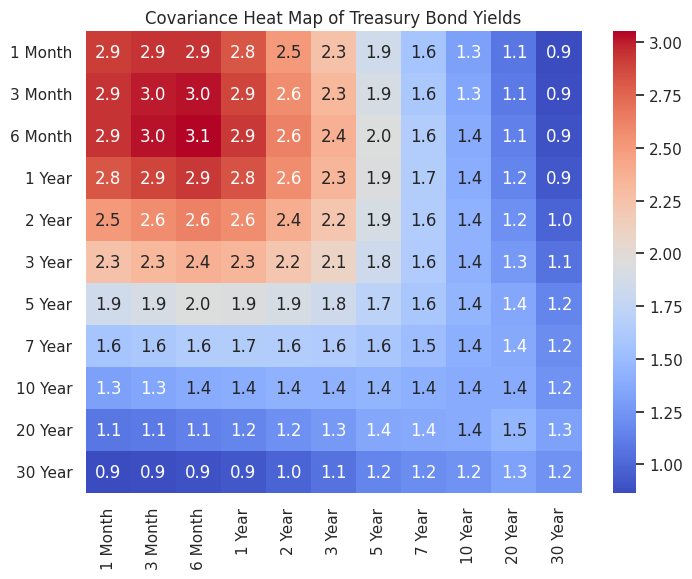
\includegraphics[width=1\textwidth]{gfx/m1l4_notes_covariance_heatmap.png}
    \caption{Bản đồ nhiệt Hiệp phương sai của Lợi suất Trái phiếu Kho bạc}
    \label{fig:m1l4_notes_covariance_heatmap}
\end{figure}

Từ bản đồ nhiệt ma trận hiệp phương sai ở trên, chúng ta có thể đọc các sự khác biệt về các giá trị hiệp phương sai một cách dễ dàng hơn. Tuy nhiên, một nhược điểm của hiệp phương sai là giá trị của nó thay đổi khi thang đo của hai biến số thay đổi. Chúng ta không thể đơn thuần so sánh các hiệp phương sai khác nhau cho các biến số theo cặp khác nhau để đánh giá xem chúng dịch chuyển cùng nhau chặt chẽ đến mức nào. Do vấn đề này, chúng ta sử dụng tương quan (correlation) thường xuyên hơn trong phân tích dữ liệu.

\subsection[Tương quan]{Tương quan (Correlation)}

Tương quan cũng là một thước đo để đánh giá sự dịch chuyển cùng chiều của hai biến số. Tuy nhiên, nó loại bỏ vấn đề về thang đo đã đề cập ở trên bằng cách chia hiệp phương sai cho căn bậc hai của tích phương sai của hai biến. Dưới đây là công thức toán học tính tương quan:

$$Corr(X,Y)=\frac{Cov(X,Y)}{\sqrt{Var(X)*Var(Y)}}$$

trong đó $Cov(X,Y)$ là hiệp phương sai của $X$ và $Y$, $Var(X)$ và $Var(Y)$ là phương sai của $X$ và $Y$.

Dưới đây là một số tính chất của tương quan:
1. Không giống như hiệp phương sai, giá trị của tương quan bị giới hạn trong khoảng từ -1 đến 1.
2. Nếu tương quan của hai biến lớn hơn 0, hai biến số có tương quan dương (positively correlated).
3. Nếu tương quan của hai biến nhỏ hơn 0, hai biến số có tương quan âm (negatively correlated).
4. Nếu hai biến có tương quan dương hoàn hảo, mức tương quan sẽ là 1.
5. Nếu hai biến có tương quan âm hoàn hảo, mức tương quan sẽ là -1.
6. Nếu mức tương quan bằng 0, hai biến không có tương quan tuyến tính.

Tương tự như với ma trận hiệp phương sai, nếu chúng ta có một số lượng biến lớn, chúng ta có thể sử dụng ma trận tương quan (correlation matrix) để trình bày các chỉ số tương quan cho các biến theo cặp. Hãy cùng tính toán ma trận tương quan cho dữ liệu lợi suất Trái phiếu Kho bạc Hoa Kỳ của chúng ta.

\begin{lstlisting}[language=Python]
In [7]: # Calculate correlation matrix for US Treasury yields in the dataset
        correlation_matrix = yields.corr()
        print("Correlation Matrix:")
        print(correlation_matrix)
\end{lstlisting}

\begin{lstlisting}[language=Python]
Correlation Matrix:
         1 Month   3 Month   6 Month   1 Year    2 Year    3 Year    5 Year \
1 Month  1.000000  0.996431  0.989556  0.978975  0.947951  0.912375  0.828580
3 Month  0.996431  1.000000  0.997062  0.989056  0.959920  0.924359  0.837981
6 Month  0.989556  0.997062  1.000000  0.996406  0.972332  0.938926  0.853025
1 Year   0.978975  0.989056  0.996406  1.000000  0.987188  0.960598  0.881951
2 Year   0.947951  0.959920  0.972332  0.987188  1.000000  0.991614  0.937754
3 Year   0.912375  0.924359  0.938926  0.960598  0.991614  1.000000  0.972950
5 Year   0.828580  0.837981  0.853025  0.881951  0.937754  0.972950  1.000000
7 Year   0.748376  0.755164  0.769085  0.800794  0.869836  0.921350  0.985414
10 Year  0.656702  0.660700  0.673469  0.705664  0.781916  0.844962  0.941356
20 Year  0.523785  0.525045  0.535579  0.568108  0.651319  0.726060  0.855190
30 Year  0.456151  0.454056  0.461334  0.492170  0.576905  0.655966  0.799992

         7 Year    10 Year   20 Year   30 Year
1 Month  0.748376  0.656702  0.523785  0.456151
3 Month  0.755164  0.660700  0.525045  0.454056
6 Month  0.769085  0.673469  0.535579  0.461334
1 Year   0.800794  0.705664  0.568108  0.492170
2 Year   0.869836  0.781916  0.651319  0.576905
3 Year   0.921350  0.844962  0.726060  0.655966
5 Year   0.985414  0.941356  0.855190  0.799992
7 Year   1.000000  0.983513  0.927076  0.885778
10 Year  0.983513  1.000000  0.976877  0.951616
20 Year  0.927076  0.976877  1.000000  0.990011
30 Year  0.885778  0.951616  0.990011  1.000000
\end{lstlisting}

Tiếp theo, hãy tạo một bản đồ nhiệt cho ma trận tương quan để dễ đọc kết quả hơn.

\begin{lstlisting}[language=Python]
In [8]: # Make a heatmap for correlation matrix
        plt.figure(figsize=(8,6))
        sns.heatmap(correlation_matrix, annot=True, cmap='coolwarm', fmt=".2f")
        plt.title('Correlation Heat Map of Treasury Bond Yields')
        plt.show()
\end{lstlisting}

\begin{figure}[htbp]
    \centering
    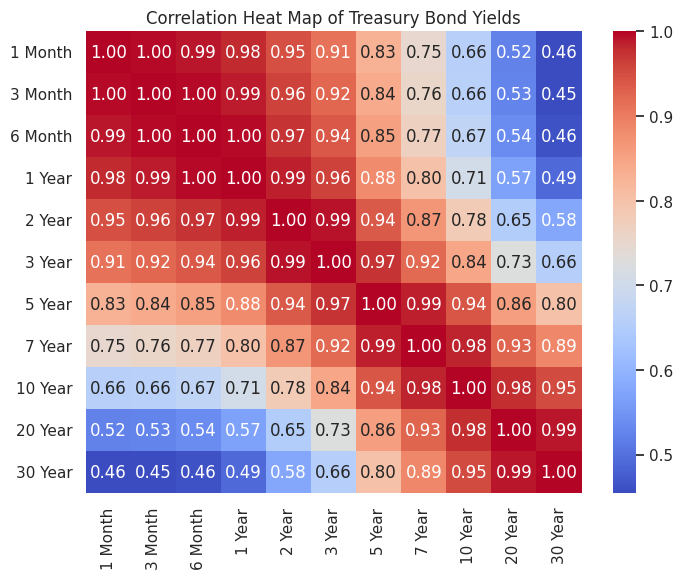
\includegraphics[width=1\textwidth]{gfx/m1l4_notes_correlation_heatmap.png}
    \caption{Bản đồ nhiệt Tương quan của Lợi suất Trái phiếu Kho bạc}
    \label{fig:m1l4_notes_correlation_heatmap}
\end{figure}

Từ bản đồ nhiệt ma trận tương quan cho lợi suất Trái phiếu Kho bạc Hoa Kỳ ở trên, chúng ta có thể so sánh tương quan giữa các cặp lợi suất khác nhau. Đầu tiên, chúng ta có thể thấy các giá trị tương quan trên các ô đường chéo đều là 1. Điều này dễ hiểu vì tất cả các mức lợi suất đều biến động hoàn toàn đồng điệu với chính nó. Thứ hai, một quan sát thú vị khác là hai lợi suất có kỳ hạn gần nhau thì có sự tương quan cao hơn. Khi khoảng cách về kỳ hạn của hai lợi suất ngày càng mở rộng, tương quan giữa hai mức lợi suất càng thấp.

Do tính chất dễ hiểu của nó, thước đo tương quan là một công cụ đo lường quan trọng và thường được sử dụng trong phân tích biến đôi. Hiểu được mối tương quan giữa lợi suất của các loại Trái phiếu Kho bạc khác nhau là điều rất quan trọng trong quản trị rủi ro, xây dựng danh mục đầu tư và thấu hiểu các động lực học của thị trường. Nó giúp định lượng cách các phần khác nhau của đường cong lợi suất dịch chuyển so với nhau, điều này đặc biệt cần thiết cho các chiến lược như giao dịch theo đường cong lợi suất và miễn nhiễm rủi ro (immunization) trong các danh mục đầu tư trái phiếu.

\section[Trích xuất Đặc trưng và Phân tích Thành phần Chính]{Trích xuất Đặc trưng và Phân tích Thành phần Chính (Feature Extractions and Principal Component Analysis)}

Trong phần này, chúng ta sẽ giới thiệu một phương pháp để trích xuất các đặc điểm chính (key features) từ một tập dữ liệu. Phương pháp này được gọi là phân tích thành phần chính (principal component analysis - PCA). Thường thì, chúng ta cố gắng phát hiện ra các nhân tố cốt lõi chung hoặc các đặc điểm có thể giải thích sự chuyển động của tất cả các biến số trong một tập dữ liệu. Nếu chúng ta có thể tìm thấy các nhân tố cốt lõi chung này - những nhân tố có khả năng đại diện cho phần lớn sự biến thiên dữ liệu trong tập dữ liệu - chúng ta sẽ không cần phải sử dụng toàn bộ tập dữ liệu để phân tích. Thay vào đó, chúng ta có thể tập trung phân tích các nhân tố cốt lõi này. Đây là một kỹ thuật giảm chiều dữ liệu (data dimension reduction technique). Việc giảm kích thước của tập dữ liệu là rất quan trọng vì nó giúp cho nhiều thuật toán hoạt động hiệu quả hơn.

Trong phần này, chúng ta sẽ tiếp tục sử dụng tập dữ liệu lợi suất Trái phiếu Kho bạc Hoa Kỳ để minh họa cho kỹ thuật này. Chúng ta sẽ trình bày từng bước một quá trình thực hiện PCA. Bước đầu tiên của chúng ta là chuẩn hóa (standardize) thang đo của các biến trong tập dữ liệu.

\subsection[Chuẩn hóa Biến số]{Chuẩn hóa Biến số (Standardizing Variables)}

Chuẩn hóa (standardizing hoặc normalizing) một biến số là một kỹ thuật thống kê phổ biến được dùng để biến đổi một biến về thang đo tiêu chuẩn. Kỹ thuật này chuyển đổi một biến số sao cho nó có giá trị trung bình là 0 và độ lệch chuẩn là 1. Dưới đây là công thức để chuẩn hóa một biến số:

$$Z=\frac{X-\mu}{\sigma}$$

Trong đó:
$Z$ = biến đã chuẩn hóa với trung bình = 0 và độ lệch chuẩn = 1
$X$ = biến ban đầu
$\mu$ = trung bình của biến ban đầu
$\sigma$ = độ lệch chuẩn của biến ban đầu

Dưới đây là các lợi ích của việc chuẩn hóa các biến:
1. Đưa tất cả các biến về cùng một thang đo để có thể so sánh được
2. Tạo điều kiện thuận lợi cho việc tính toán các phân tích khác yêu cầu các biến ở cùng một thang đo

Bây giờ chúng ta hãy chuẩn hóa tập dữ liệu lợi suất Trái phiếu Kho bạc Hoa Kỳ. Trước tiên chúng ta cần tính giá trị trung bình và độ lệch chuẩn của từng mức lợi suất. Sau đó, chúng ta sẽ áp dụng công thức trên vào tập dữ liệu để tạo ra một tập dữ liệu đã được chuẩn hóa.

\begin{lstlisting}[language=Python]
In [9]: # Calculate means for all yields in the dataset
        yield_means = yields.mean()
        print("Yield Means:")
        print(yield_means)
\end{lstlisting}

\begin{lstlisting}[language=Python]
Yield Means:
1 Month     1.449053
3 Month     1.518396
6 Month     1.627451
1 Year      1.717973
2 Year      1.905475
3 Year      2.097270
5 Year      2.485802
7 Year      2.806259
10 Year     3.088349
20 Year     3.620395
30 Year     3.724571
dtype: float64
\end{lstlisting}

\begin{lstlisting}[language=Python]
In [10]: # Calculate standard deviations for all yields in the dataset
         yield_stds = yields.std()
         print("Yield Standard Deviations:")
         print(yield_stds)
\end{lstlisting}

\begin{lstlisting}[language=Python]
Yield Standard Deviations:
1 Month     1.705851
3 Month     1.733347
6 Month     1.746829
1 Year      1.684091
2 Year      1.545413
3 Year      1.446639
5 Year      1.309345
7 Year      1.226457
10 Year     1.174092
20 Year     1.206514
30 Year     1.108774
dtype: float64
\end{lstlisting}

\begin{lstlisting}[language=Python]
In [11]: # Now create a standardized US Treasury yield dataset
         standardized_data = (yields - yield_means) / yield_stds
         print("Standardized Yield (first 5 rows):")
         print(standardized_data.head())
\end{lstlisting}

\begin{lstlisting}[language=Python]
Standardized Yield (first 5 rows):
             1 Month   3 Month   6 Month    1 Year    2 Year    3 Year \
2001-07-31  1.301958  1.166300  1.054796  1.075968  1.219431  1.356751
2001-08-01  1.290234  1.160531  1.054796  1.093781  1.245314  1.377489
2001-08-02  1.290234  1.160531  1.049071  1.099719  1.284139  1.432789
2001-08-03  1.278510  1.154762  1.054796  1.099719  1.297080  1.467352
2001-08-06  1.272647  1.154762  1.054796  1.093781  1.277668  1.432789

              5 Year    7 Year   10 Year   20 Year   30 Year
2001-07-31  1.591786  1.674532  1.687817  1.649052  1.610273
2001-08-01  1.629973  1.707147  1.721886  1.665629  1.628311
2001-08-02  1.683435  1.764222  1.772989  1.707071  1.664387
2001-08-03  1.706348  1.780529  1.798541  1.723647  1.682425
2001-08-06  1.698710  1.780529  1.790023  1.723647  1.682425
\end{lstlisting}

Thông thường, việc chuẩn bị một tập dữ liệu đã chuẩn hóa là một phần trong bước chuẩn bị dữ liệu trước khi chạy phân tích. Hãy đảm bảo rằng bạn đã chuẩn hóa tập dữ liệu của mình nếu thuật toán phân tích mà bạn sắp chạy đòi hỏi các biến phải ở cùng một thang đo.

Trước khi chuyển sang bước tiếp theo của thuật toán PCA, chúng ta cần tìm hiểu các công cụ mới từ đại số tuyến tính. Trong hai phần tiếp theo, chúng ta sẽ giới thiệu các vector riêng (eigenvectors) và các trị riêng (eigenvalues).

\subsection[Vector Riêng và Trị Riêng]{Vector Riêng và Trị Riêng (Eigenvectors and Eigenvalues)}

Trong phần này, chúng ta sẽ tìm hiểu định nghĩa của các vector riêng và trị riêng cũng như cách tính toán chúng. Phân tích đặc trưng (eigenanalysis) là một phương pháp đại số tuyến tính rất quan trọng trong tài chính. Hãy xem lại phần tài liệu đọc bắt buộc của bài học này để hiểu rõ hơn về chủ đề này. Trong phần tiếp theo, chúng ta sẽ sử dụng phương pháp trực quan hóa để nâng cao hiểu biết về vector riêng và trị riêng.

\subsection[Trực quan hóa Vector riêng và Trị riêng]{Trực quan hóa Vector riêng và Trị riêng (Visualization of Eigenvectors and Eigenvalues)}

Trong phần này, chúng ta sẽ sử dụng đồ thị để giải thích các khái niệm về vector riêng và trị riêng.

Các vector trong một hệ tọa độ hai chiều được mô tả bởi độ lớn (magnitude) và hướng (direction) của chúng. Một phép biến đổi tuyến tính (linear transformation) xảy ra khi chúng ta nhân một vector với một ma trận. Phép biến đổi có thể làm thay đổi cả độ lớn và hướng của vector đó. Tuy nhiên, có những vector đặc biệt duy trì được hướng của chúng hoặc chỉ đảo chiều ngược lại khi một phép biến đổi tuyến tính xảy ra. Sự thay đổi duy nhất là về độ lớn của các vector này. Những vector đặc biệt này được gọi là vector riêng (eigenvectors). Đầu tiên, hãy xem lại phương trình giữa các vector riêng và trị riêng ở chương trước:

$$Ax=\lambda x$$

Trong đó:
$A$ là ma trận biến đổi tuyến tính
$x$ là vector riêng
$\lambda$ là số liệu đo lường độ lớn hoặc trị riêng

Đầu tiên, hãy nhìn vào vế trái của phương trình. Nó tương ứng với phép biến đổi tuyến tính của một vector mà chúng ta đã mô tả ở trên. Ở vế phải, vector này nhân với một số vô hướng (scalar). Khi vế trái của phương trình bằng vế phải của phương trình, điều đó có nghĩa là phép biến đổi tuyến tính của vector đó bằng với sự thay đổi độ lớn của chính vector đó. Dựa trên những gì chúng ta mô tả về một vector riêng, vector trong phương trình này chính là một vector riêng. Hình 1 bên dưới minh họa trực quan khái niệm này.

\textbf{Hình 1: Trực quan hóa về Vector riêng và Trị riêng} \\
\textit{Biểu đồ minh họa phép biến đổi tuyến tính của một hệ tọa độ (x, y) với một đường tròn được biến đổi thành một hình elip, đánh dấu vector riêng $v_1$ và phiên bản phóng to của nó $\lambda v_1$}

Từ hình vẽ trên, chúng ta có thể thấy vector riêng màu tím vẫn giữ nguyên hướng của nó sau phép biến đổi tuyến tính, được thể hiện bằng vector màu cam. Phép biến đổi chỉ đơn thuần làm giãn ra hoặc nén lại vector riêng mà không làm thay đổi hướng của nó.

Trị riêng (eigenvalue) liên kết với một vector riêng là con số cho biết vector riêng đó được điều chỉnh tỷ lệ bao nhiêu trong quá trình biến đổi.
\begin{itemize}
    \item Nếu trị riêng dương, vector riêng được kéo giãn theo hướng ban đầu.
    \item Nếu âm, vector riêng được kéo giãn theo hướng ngược lại.
    \item Nếu trị riêng bằng 1, vector riêng không thay đổi.
    \item Nếu bằng 0, vector riêng bị thu gọn thành một điểm. Khi biểu diễn các trị riêng dưới dạng độ dài của vector, độ dài của mỗi mũi tên vector riêng có thể được thay đổi theo tỷ lệ để thể hiện trị riêng tương ứng của nó.
\end{itemize}

\subsection[Rút trích các Thành phần Chính]{Rút trích các Thành phần Chính (Derive Principal Components)}

Bước tiếp theo của thuật toán PCA là tìm ma trận hiệp phương sai của tập dữ liệu đã được chuẩn hóa. Đối với một tập dữ liệu đã chuẩn hóa, ma trận hiệp phương sai của nó sẽ hoàn toàn giống với ma trận tương quan của tập dữ liệu trước khi chuẩn hóa. Trong đoạn mã Python sau đây, trước tiên chúng ta import các thư viện cần thiết để thao tác với ma trận và để tính toán các vector riêng/trị riêng. Sau đó, chúng ta sẽ lấy ma trận hiệp phương sai cho dữ liệu đã chuẩn hóa và vẽ bản đồ nhiệt cho ma trận hiệp phương sai này.

\begin{lstlisting}[language=Python]
In [12]: import numpy as np
         from numpy import linalg as LA
\end{lstlisting}

\begin{lstlisting}[language=Python]
In [13]: # Calculate covariance matrix of the standardized dataset
         std_data_cov = standardized_data.cov()
\end{lstlisting}

\begin{lstlisting}[language=Python]
In [14]: # Draw a heatmap of the covariance matrix
         plt.figure(figsize=(8,6))
         sns.heatmap(std_data_cov, annot=True, cmap='coolwarm', fmt=".2f")
         plt.title('Covariance Heat Map of Standardized Treasury Bond Yields')
         plt.show()
\end{lstlisting}

\begin{figure}[htbp]
    \centering
    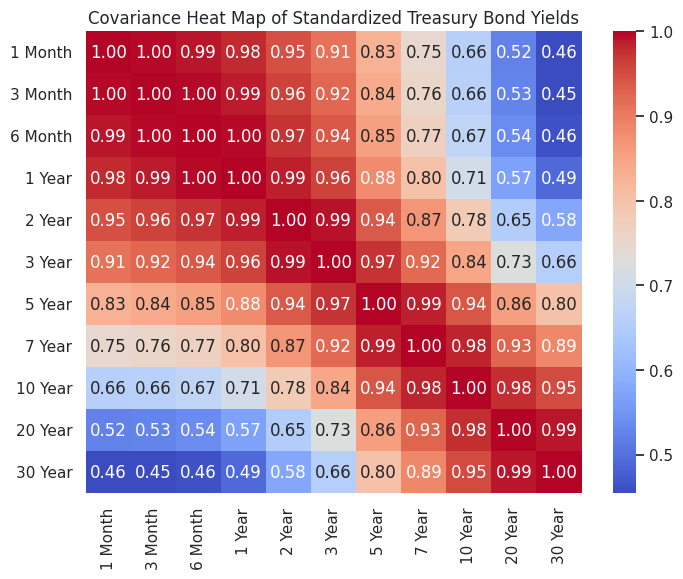
\includegraphics[width=1\textwidth]{gfx/m1l4_notes_covariance_heatmap_standardized.png}
    \caption{Bản đồ nhiệt Hiệp phương sai của Lợi suất Trái phiếu Kho bạc đã Chuẩn hóa}
    \label{fig:m1l4_notes_covariance_heatmap_standardized}
\end{figure}

Bây giờ chúng ta hãy tính toán các vector riêng và trị riêng của ma trận hiệp phương sai của tập dữ liệu lợi suất đã được chuẩn hóa.

\begin{lstlisting}[language=Python]
In [15]: # Calculate eigenvectors and eigenvalues of the covariance matrix of standar
         eigenvalues, eigenvectors = LA.eig(std_data_cov)
         eigenvalues
\end{lstlisting}

\begin{lstlisting}[language=Python]
Out [15]: array([9.22236235e+00, 1.63341019e+00, 1.17347718e-01, 1.46747161e-02,
                 5.37172584e-03, 3.70149555e-03, 1.61309240e-03, 6.97458739e-04,
                 4.12103724e-04, 2.47130907e-04, 1.62022336e-04])
\end{lstlisting}

\begin{lstlisting}[language=Python]
In [16]: eigenvectors
\end{lstlisting}

\begin{lstlisting}[language=Python]
Out [16]: array([[ 0.44114252,  0.16709103, -0.53274513,  0.29838306,  0.30407626,
                  -0.06687106,  0.02716335,  0.33473909, -0.24039038,  0.3702677 ,
                  -0.00401581],
                 [ 0.30709453,  0.3256805 ,  0.3004742 , -0.10407045, -0.09017425,
                  -0.45363295,  0.58333199, -0.13905681, -0.13428768,  0.31674937,
                   0.08135824],
                 [ 0.30335843,  0.29873569,  0.17614053,  0.25730089, -0.24045099,
                  -0.34295333, -0.10807462, -0.13460411,  0.32846299, -0.58367918,
                  -0.26019232],
                 [ 0.42112655, -0.09742097, -0.00945148,  0.26727645,  0.30894871,
                  -0.16475673,  0.38500876,  0.15471834, -0.48093818, -0.17006916,
                   0.43202651],
                 [ 0.31879358,  0.17616334, -0.28944958,  0.31333639,  0.25331718,
                   0.2316792 ,  0.23709616,  0.21742618, -0.3594238 ,  0.02750551,
                  -0.57801452],
                 [ 0.32383758,  0.08574516, -0.41253571,  0.06981027,  0.2557664 ,
                   0.27857918, -0.04283274,  0.253605  ,  0.24613993, -0.32221553,
                   0.58235483],
                 [ 0.32393331, -0.09082567, -0.38335179, -0.28984745,  0.02440707,
                   0.41667104, -0.0335848 , -0.25924506, -0.22190129,  0.51816781,
                  -0.30913315],
                 [ 0.31475338, -0.2155924 , -0.25536488, -0.38788729, -0.13245802,
                  -0.19980121, -0.25664372, -0.23752598, -0.60974821, -0.28958861,
                   0.05811859],
                 [ 0.27752025,  0.29830301, -0.32947806, -0.0224116 , -0.14078023,
                   0.07495589, -0.36651204,  0.64790245,  0.35934669,  0.10798909,
                   0.06783763],
                 [-0.48820444,  0.2677569 , -0.44896794,  0.22584655,  0.25821905,
                   0.02106533,  0.58883593, -0.14816743, -0.03038806,  0.00408296,
                  -0.02532805],
                 [ 0.24905042, -0.49930724,  0.38802724,  0.65844796,  0.19437911,
                  -0.01338036,  0.03078012, -0.21614344, -0.11702391, -0.07221199,
                   0.00323551]])
\end{lstlisting}

Từ output trên, chúng ta có thể thấy các trị riêng và các vector riêng tương ứng của nó đã được sắp xếp theo thứ tự giảm dần dựa trên giá trị của trị riêng. Trong thuật toán PCA, chúng ta cũng gọi các vector riêng là tải số (loadings). Chúng ta sẽ hiểu lý do tại sao điều này lại quan trọng ở phần sau.

Chúng ta có thể coi bộ sưu tập tất cả các vector riêng này như một ma trận biến đổi tuyến tính đối với tập dữ liệu đã chuẩn hóa. Dữ liệu đã được biến đổi này sẽ có một đặc tính rất thú vị mà chúng ta sẽ sớm giới thiệu. Đầu tiên, hãy biến đổi dữ liệu đã chuẩn hóa bằng các vector riêng.

\begin{lstlisting}[language=Python]
In [17]: # Transform standardized data with Loadings
         principal_components = standardized_data.dot(eigenvectors)
         principal_components.columns = ["PC_1", "PC_2", "PC_3", "PC_4", "PC_5", "PC_6",
         principal_components.head()
\end{lstlisting}

\begin{lstlisting}[language=Python]
Out [17]:             PC_1      PC_2      PC_3      PC_4      PC_5      PC_6      PC_7
          2001-07-31  4.608202 -0.918184  0.138746 -0.223360  0.013690  0.063247  0.008572
          2001-08-01  4.665170 -0.950595  0.102492 -0.220182  0.013318  0.054096  0.014505
          2001-08-02  4.766161 -1.009754  0.054519 -0.230244  0.021179  0.064157  0.017119
          2001-08-03  4.807092 -1.038602  0.027695 -0.224234  0.025575  0.063723  0.018644
          2001-08-06  4.781112 -1.044855  0.048161 -0.228694  0.013594  0.051783  0.009102
\end{lstlisting}

Kết quả trên hiển thị 11 biến đã được biến đổi. Trong PCA, chúng được gọi là các thành phần chính (principal components). Hãy nhớ rằng chúng ta đã đề cập trước đó rằng các trị riêng từ PCA được sắp xếp theo thứ tự giảm dần. Những thành phần chính này cũng được trình bày theo cùng trình tự như các trị riêng tương ứng của chúng. Ví dụ, PC\_1 tương ứng với trị riêng đầu tiên, có giá trị là 9.22. PC\_2 tương ứng với trị riêng cao thứ hai, có giá trị là 1.63.

Đặc trưng quan trọng nhất của PCA là các thành phần chính đứng đầu có khả năng giải thích một tỷ lệ phương sai của tập dữ liệu cao hơn so với các thành phần chính còn lại. Ví dụ, PC\_1 có thể giải thích được nhiều sự biến thiên trong dữ liệu đã chuẩn hóa hơn so với PC\_2. Nhưng là bao nhiêu? Trị riêng tương ứng cho PC\_1 chính là lượng phương sai của toàn bộ dữ liệu mà PC\_1 giải thích được. Nó có giá trị 9.22 trong trường hợp này. Theo cùng một logic, PC\_2 giải thích 1.63 trong tổng phương sai của tập dữ liệu. Chúng ta có thể cộng tất cả các trị riêng lại để có được tổng phương sai của dữ liệu. Từ tổng phương sai của dữ liệu, chúng ta cũng có thể tính được tỷ lệ phần trăm đóng góp vào phương sai mà mỗi thành phần chính nắm bắt được. Dưới đây là mã Python.

\begin{lstlisting}[language=Python]
In [18]: # Put data into a DataFrame
         df_eigval = pd.DataFrame({"Eigenvalues": eigenvalues}, index=range(1,12))
         # Work out explained proportion
         df_eigval["Explained proportion"] = df_eigval["Eigenvalues"] / np.sum(eigenv
         #Format as percentage
         df_eigval.style.format({"Explained proportion": "{:.2%}"})
\end{lstlisting}

\begin{lstlisting}[language=Python]
Out [18]:      Eigenvalues  Explained proportion
          1     9.222362      83.84%
          2     1.633410      14.85%
          3     0.117348       1.07%
          4     0.014675       0.13%
          5     0.005372       0.05%
          6     0.003701       0.03%
          7     0.001613       0.01%
          8     0.000697       0.01%
          9     0.000412       0.00%
          10    0.000247       0.00%
          11    0.000162       0.00%
\end{lstlisting}

Từ bảng trên, chúng ta có thể thấy PC\_1 có thể giải thích gần 84\% phương sai trong tập dữ liệu đã chuẩn hóa. PC\_2 có thể giải thích gần 15\% phương sai trong dữ liệu đã chuẩn hóa. Hai thành phần chính đầu tiên này có thể giải thích tới gần 99\% sự biến thiên trong tập dữ liệu. 9 thành phần chính còn lại chỉ giải thích vỏn vẹn 1\% phương sai của dữ liệu. Vì vậy, để phân tích dữ liệu hiệu quả hơn mà không làm mất đi quá nhiều thông tin, chúng ta có thể chỉ sử dụng hai thành phần chính đầu tiên cho việc phân tích thay vì dùng tất cả 11 thành phần chính. Bởi tính chất đặc biệt này, chúng ta cũng gọi PCA là một kỹ thuật giảm chiều dữ liệu.

Phạm vi ứng dụng của PCA rất rộng trong phân tích tài chính và học máy (machine learning). Ví dụ, trong phân tích hình ảnh, bộ sưu tập hình ảnh gốc có thể rất lớn, nhưng bằng cách sử dụng PCA, chúng ta có thể giảm kích thước dữ liệu mà vẫn giữ nguyên được những đặc trưng chính của các hình ảnh.

\subsection{Phân tích Thành phần Chính cho Lợi suất Trái phiếu Kho bạc Hoa Kỳ}

Điều tuyệt vời của việc sử dụng PCA để phân tích đường cong lợi suất Trái phiếu Kho bạc Hoa Kỳ là nó có thể phân tách đường cong lợi suất thành một số các thành phần chính (Oprea). Ba thành phần chính dẫn đầu mô tả các đặc điểm sau đây của đường cong lợi suất:
1. PC\_1: sự dịch chuyển song song của đường cong lợi suất (shift).
2. PC\_2: sự dẹt đi (flattening) hoặc dốc hơn (steeping) của đường cong lợi suất (tilt).
3. PC\_3: sự thay đổi độ cong của đường cong lợi suất (twist).

Đầu tiên, hãy vẽ đường cong lợi suất làm tiêu chuẩn để so sánh tốt hơn (Bjerring).

\begin{lstlisting}[language=Python]
In [19]: # Treasury Yield Curve
         yields.plot(figsize=(12, 8), title='Figure 2, Treasury Yields', alpha=0.7) #
         plt.legend(bbox_to_anchor=(1.03,1))
         plt.show()
\end{lstlisting}

\begin{figure}[htbp]
    \centering
    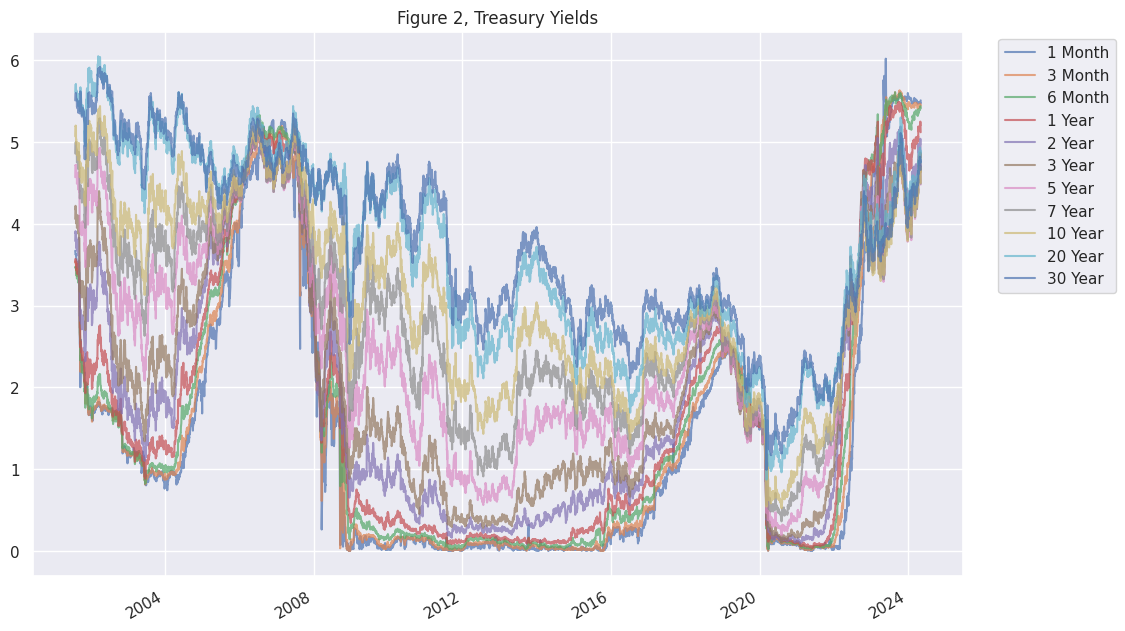
\includegraphics[width=1\textwidth]{gfx/m1l4_notes_fig2_treasury_yields.png}
    \caption{Hình 2, Lợi suất Trái phiếu Kho bạc}
    \label{fig:m1l4_notes_fig2_treasury_yields}
\end{figure}

Bây giờ, hãy vẽ các thành phần chính. Bắt đầu với PC\_1.

\begin{lstlisting}[language=Python]
In [20]: # Plot PC_1
         principal_components["PC_1"].plot(figsize=(12,8), title='Figure 3, Principa
         plt.show()
\end{lstlisting}

\begin{figure}[htbp]
    \centering
    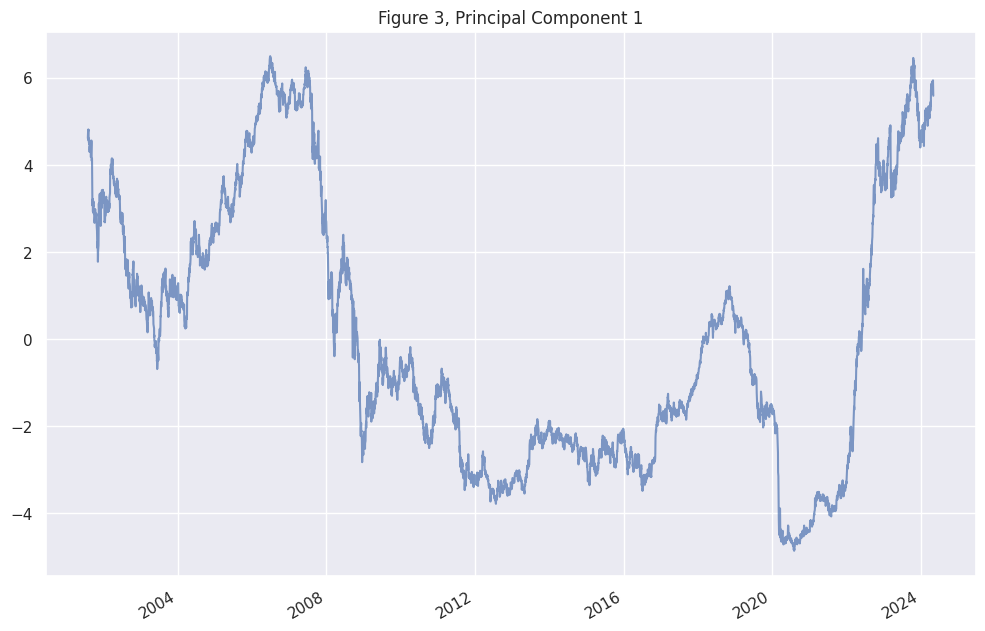
\includegraphics[width=1\textwidth]{gfx/m1l4_notes_fig3_pc1.png}
    \caption{Hình 3, Thành phần Chính 1}
    \label{fig:m1l4_notes_fig3_pc1}
\end{figure}

Từ Hình 3 của PC\_1 ở trên, chúng ta có thể thấy mô hình (pattern) trông tương tự với mô hình của Hình 2 (biểu đồ này bắt đầu từ năm 2001 vì chúng ta đã loại bỏ dữ liệu NaN). PC\_1 này được dùng để thể hiện sự dịch chuyển song song của đường cong lợi suất. Tiếp theo, hãy phân tích PC\_2. PC\_2 thường được dùng để phân tích xem đường cong lợi suất bị nghiêng (tilted) như thế nào. Minh họa bằng mã Python sau đây sẽ giải thích lý do tại sao PC\_2 lại được dùng để phân tích độ nghiêng (tilt).

Đầu tiên, hãy tính toán sự chênh lệch giữa lợi suất 2 năm và lợi suất 10 năm như là độ nghiêng của đường cong lợi suất và vẽ một đồ thị.

\begin{lstlisting}[language=Python]
In [21]: # Calculate slope (difference) of 2-year Treasury yield and 10-year Treasury
         df_s = pd.DataFrame(data = standardized_data)
         df_s = df_s[["2 Year", "10 Year"]]
         df_s["Tilt"] = df_s["2 Year"] - df_s["10 Year"]
         df_s.head()
\end{lstlisting}

\begin{lstlisting}[language=Python]
Out [21]:              2 Year   10 Year      Tilt
          2001-07-31 1.219431  1.687817 -0.468386
          2001-08-01 1.245314  1.721886 -0.476571
          2001-08-02 1.284139  1.772989 -0.488850
          2001-08-03 1.297080  1.798541 -0.501460
          2001-08-06 1.277668  1.790023 -0.512355
\end{lstlisting}

\begin{lstlisting}[language=Python]
In [22]: # Draw the graph of Slope of 2-Year Treasury Yield - 10-Year Treasury Yield
         df_s["Tilt"].plot(figsize=(12,8), title='Figure 4, Tilt of 2-Year Treasury 
         plt.show()
\end{lstlisting}

\begin{figure}[htbp]
    \centering
    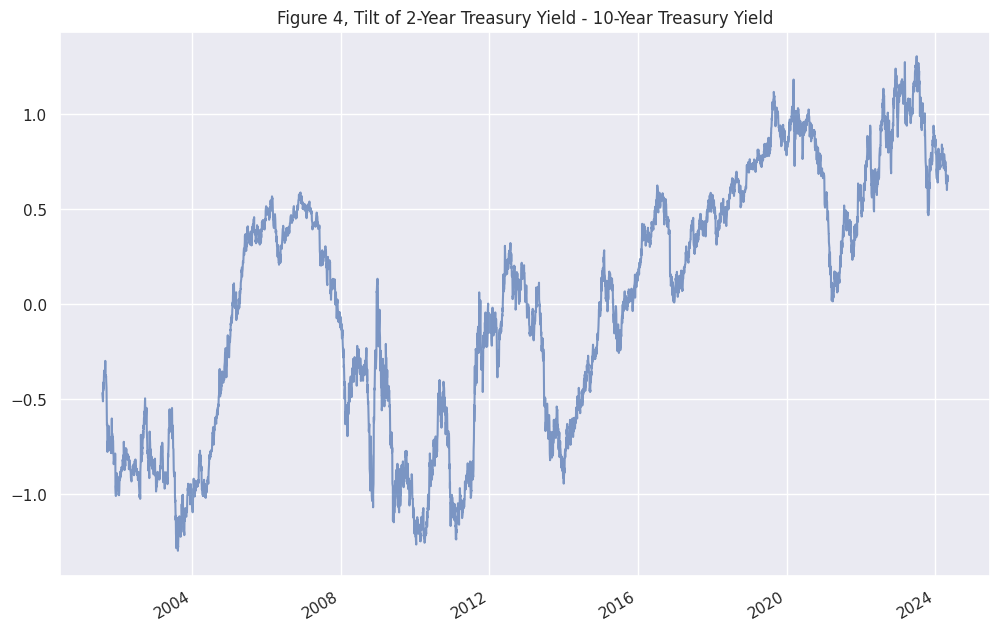
\includegraphics[width=1\textwidth]{gfx/m1l4_notes_fig4_tilt_2y10y.png}
    \caption{Hình 4, Độ nghiêng của Lợi suất Trái phiếu Kho bạc 2 Năm - Lợi suất Trái phiếu Kho bạc 10 Năm}
    \label{fig:m1l4_notes_fig4_tilt_2y10y}
\end{figure}

Sau khi vẽ Hình 4 về mức chênh lệch lợi suất giữa lợi suất Trái phiếu Kho bạc 2 năm và lợi suất Trái phiếu Kho bạc 10 năm, chúng ta hãy vẽ đồ thị cho PC\_2.

\begin{lstlisting}[language=Python]
In [23]: # Draw the graph for PC_2
         principal_components["PC_2"].plot(figsize=(12,8), title='Figure 5, Principa
         plt.show()
\end{lstlisting}

\begin{figure}[htbp]
    \centering
    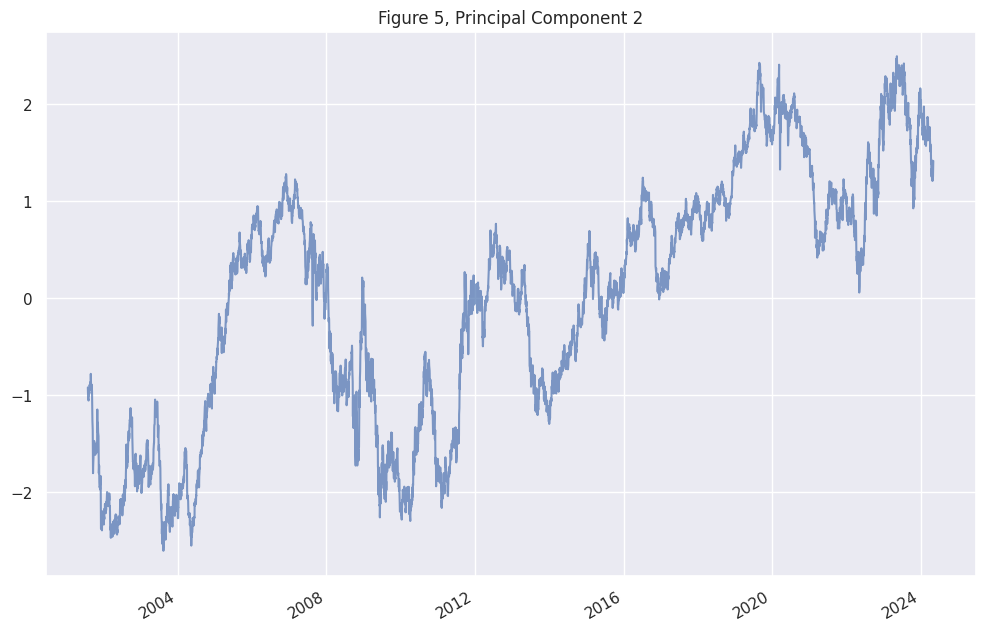
\includegraphics[width=1\textwidth]{gfx/m1l4_notes_fig5_pc2.png}
    \caption{Hình 5, Thành phần Chính 2}
    \label{fig:m1l4_notes_fig5_pc2}
\end{figure}

Từ Hình 4 và Hình 5, chúng ta có thể thấy biểu đồ độ nghiêng (tilt) của lợi suất Trái phiếu Kho bạc 2 năm và lợi suất 10 năm có mô hình tương tự như biểu đồ PC\_2. Hãy tính tương quan để xác nhận quan sát này.

\begin{lstlisting}[language=Python]
In [24]: np.corrcoef(principal_components["PC_2"], df_s["Tilt"])
\end{lstlisting}

\begin{lstlisting}[language=Python]
Out [24]: array([[1.        , 0.97850538],
                 [0.97850538, 1.        ]])
\end{lstlisting}

Đoạn code trên cho thấy rằng tương quan giữa PC\_2 và Độ nghiêng (Tilt) là 97\%, đây là mức rất cao. Vì vậy, chúng ta có thể sử dụng PC\_2 làm đại diện (proxy) để phân tích xem đường cong lợi suất đang nghiêng (tilted) như thế nào.

Bây giờ chúng ta hãy vẽ PC\_3, sự thay đổi độ cong của đường cong lợi suất.

\begin{lstlisting}[language=Python]
In [25]: # Draw the graph for PC_3
         principal_components["PC_3"].plot(figsize=(12,8), title='Figure 6, Principa
         plt.show()
\end{lstlisting}

\begin{figure}[htbp]
    \centering
    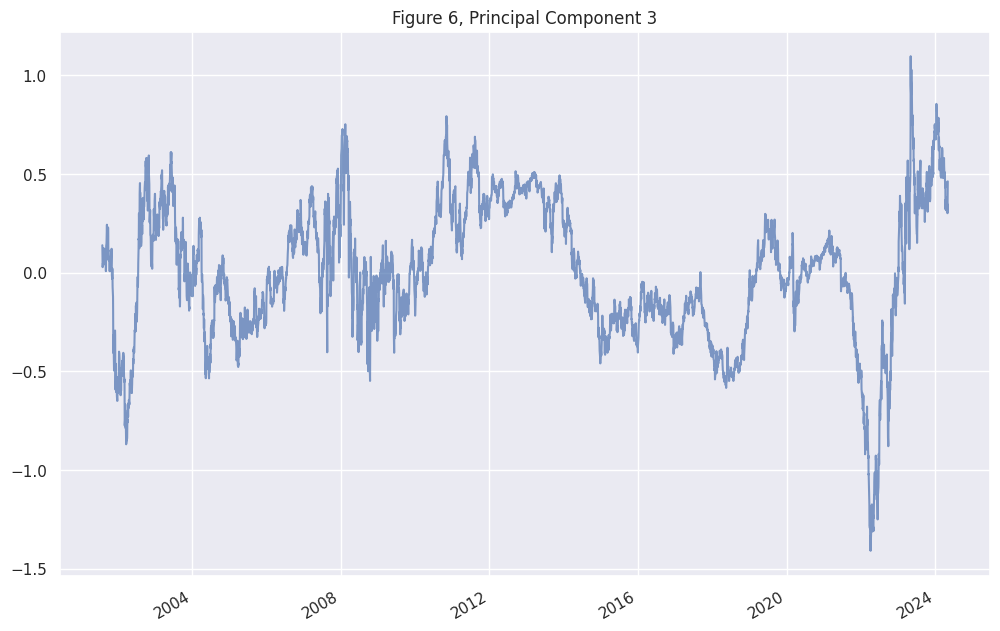
\includegraphics[width=1\textwidth]{gfx/m1l4_notes_fig6_pc3.png}
    \caption{Hình 6, Thành phần Chính 3}
    \label{fig:m1l4_notes_fig6_pc3}
\end{figure}

Từ Hình 6, chúng ta có thể thấy rằng sự thay đổi độ cong của đường cong lợi suất dao động quanh mức 0.

\section[Giá trị Rủi ro cho một Danh mục Đầu tư Có Thu nhập Cố định]{Giá trị Rủi ro (Value at Risk) cho một Danh mục Đầu tư Có Thu nhập Cố định}

Trong phần này, chúng ta sẽ sử dụng phương pháp trích xuất đặc trưng mà chúng ta đã học ở phần trước để tính toán Giá trị Rủi ro (Value at Risk) của một danh mục đầu tư trái phiếu.

\subsection[Giá trị Rủi ro]{Giá trị Rủi ro (Value at Risk - VaR)}

Giá trị Rủi ro (VaR) là một thước đo thống kê để đánh giá mức độ tổn thất tối đa tiềm tàng của một khoản đầu tư hay một danh mục đầu tư trong một khoảng thời gian xác định dưới một mức độ tin cậy (confidence level) nhất định. Ví dụ, khi một danh mục đầu tư cổ phiếu có VaR là 1 triệu đô la trong một ngày ở mức độ tin cậy 95\%, điều đó có nghĩa là có 95\% xác suất danh mục đầu tư cổ phiếu này sẽ không mất hơn 1 triệu đô la trong một ngày.

VaR là một chỉ số rủi ro dễ hiểu và có thể được sử dụng để so sánh rủi ro trên các nhóm tài sản khác nhau. VaR thường được sử dụng trong quản trị rủi ro đối với quản lý danh mục đầu tư hoặc cho các báo cáo quy định. Nó cũng là một phần của các thước đo nhằm thiết lập mức trần rủi ro (risk cap) cho các nhà giao dịch. VaR cũng có thể được áp dụng cho việc phân bổ vốn.

\subsection{VaR đối với một Danh mục Đầu tư Trái phiếu Kho bạc Đơn giản}

Chúng ta sẽ chỉ ra cách tính VaR cho một danh mục đầu tư Trái phiếu Kho bạc đơn giản trong phần này. Danh mục đầu tư trái phiếu đơn giản này sẽ chỉ bao gồm Trái phiếu Kho bạc kỳ hạn 2 năm, Trái phiếu Kho bạc kỳ hạn 5 năm, và Trái phiếu Kho bạc kỳ hạn 10 năm. Đầu tiên, hãy tạo một tập dữ liệu với lợi suất của ba trái phiếu này và tính tỷ lệ phần trăm thay đổi lợi suất hàng ngày của chúng.

\begin{lstlisting}[language=Python]
In [26]: # Create a dataset with 3 Treasury bond yields and calculate the yield chang
         var_dataset = yields[["2 Year", "5 Year", "10 Year"]]
         var_yield_chng_dataset = var_dataset.pct_change()
         var_yield_chng_dataset = var_yield_chng_dataset.dropna()
         var_yield_chng_dataset.head()
\end{lstlisting}

\begin{lstlisting}[language=Python]
Out [26]:               2 Year    5 Year   10 Year
          2001-08-01  0.010554  0.010941  0.007890
          2001-08-02  0.015666  0.015152  0.011742
          2001-08-03  0.005141  0.006397  0.005803
          2001-08-06 -0.007673 -0.002119 -0.001923
          2001-08-07  0.005155  0.002123  0.001927
\end{lstlisting}

Tiếp theo, chúng ta sẽ chuẩn bị tập dữ liệu. Đầu tiên chúng ta cần chuẩn hóa dữ liệu.

\begin{lstlisting}[language=Python]
In [27]: # Standardize the dataset
         var_yield_chng_dataset_means = var_yield_chng_dataset.mean()
         var_yield_chng_dataset_stds = var_yield_chng_dataset.std()
         var_yld_chng_stnd_data = (var_yield_chng_dataset - var_yield_chng_dataset_me
\end{lstlisting}

Bây giờ chúng ta có thể tính toán các vector riêng và trị riêng của tập dữ liệu đã được chuẩn hóa.

\begin{lstlisting}[language=Python]
In [28]: # Calculate eienvectors and eigenvalues and rank by eigenvalues
         var_cov_matrix = var_yld_chng_stnd_data.cov()
         eigenvalues, eigenvectors = np.linalg.eig(var_cov_matrix)
         sorted_indices = np.argsort(eigenvalues)[::-1]
         pca_components = eigenvectors[:, sorted_indices]
\end{lstlisting}

Hãy cùng kiểm tra các trị riêng và xem mỗi vector riêng có khả năng giải thích bao nhiêu phần trăm phương sai của dữ liệu.

\begin{lstlisting}[language=Python]
In [29]: # Put data into a DataFrame
         df_eigval = pd.DataFrame({"Eigenvalues": eigenvalues}, index=range(1,4))
         # Work out explained proportion
         df_eigval["Explained proportion"] = df_eigval["Eigenvalues"] / np.sum(eigenv
         #Format as percentage
         df_eigval.style.format({"Explained proportion": "{:.2%}"})
\end{lstlisting}

\begin{lstlisting}[language=Python]
Out [29]:      Eigenvalues  Explained proportion
          1     2.545146      84.84%
          2     0.384763      12.83%
          3     0.070091       2.34%
\end{lstlisting}

Từ bảng trên, chúng ta có thể thấy hai vector riêng đầu tiên chiếm tới 97\% phương sai trong tập dữ liệu. Vì vậy, chúng ta sẽ chọn hai vector riêng đầu tiên này để phân tích.

\begin{lstlisting}[language=Python]
In [30]: # Choose number of components (e.g., 2)
         n_components = 2
         selected_components = pca_components[:, :n_components]
\end{lstlisting}

Tiếp theo, hãy giả sử rằng danh mục đầu tư trái phiếu đơn giản của chúng ta bao gồm 2 triệu đô la Trái phiếu Kho bạc kỳ hạn 2 năm, 2 triệu đô la Trái phiếu Kho bạc kỳ hạn 5 năm, và 1 triệu đô la Trái phiếu Kho bạc kỳ hạn 10 năm.

\begin{lstlisting}[language=Python]
In [31]: # Define a simple portfolio
         portfolio = {
             2: 2000000,   # $2M in 2-year bond
             5: 2000000,   # $2M in 5-year bond
             10: 1000000   # $1M in 10-year bond
         }
\end{lstlisting}

Tiếp đến, chúng ta sẽ tính các độ nhạy cảm của trái phiếu (bond sensitivities) trong danh mục đầu tư. Để đơn giản hóa, chúng ta giả định khoảng thời gian đáo hạn bình quân (duration) của trái phiếu bằng đúng kỳ hạn của chúng. Khi đó, chúng ta có thể tính được những thay đổi về giá trị của danh mục đầu tư và VaR.

\begin{lstlisting}[language=Python]
In [32]: # Calculate portfolio sensitivities (assuming duration = maturity for simpli
         sensitivities = np.array([maturity * amount for maturity, amount in portfoli
         
         # Calculate portfolio value changes
         portfolio_changes = (var_yield_chng_dataset * sensitivities) @ selected_compor
         
         # Calculate VaR
         confidence_level = 0.95 # 95% VaR
         var = -np.percentile(portfolio_changes, 100 * (1 - confidence_level))
         print(f"1-day 95% VaR: ${var:,.2f}")
         
         # Display summary statistics
         print("\nSummary Statistics:")
         print(f"Portfolio Value: ${sum(portfolio.values()):,.2f}")
         print(f"VaR as % of Portfolio Value: {var / sum(portfolio.values()) * 100:.3f}%")
\end{lstlisting}

\begin{lstlisting}[language=Python]
1-day 95% VaR: $458,248.59

Summary Statistics:
Portfolio Value: $5,000,000.00
VaR as % of Portfolio Value: 9.165%
\end{lstlisting}

Kết quả trên cho thấy VaR 1 ngày ở mức độ tin cậy 95\% cho danh mục đầu tư Trái phiếu Kho bạc đơn giản của chúng ta là \$458.249. Con số này tương đương khoảng 9\% tổng giá trị danh mục đầu tư. Ví dụ trên minh họa cách sử dụng phương pháp trích xuất đặc trưng để thu gọn tập dữ liệu danh mục đầu tư và sử dụng tập dữ liệu nhỏ hơn đó để tính toán VaR.

\section[Kết luận]{Kết luận (Conclusion)}

Trong bài học này, trước tiên chúng ta đã đi qua những kiến thức cơ bản về phân tích biến đôi. Chúng ta đã giải thích phân tích biến đôi là gì và sau đó giới thiệu các khái niệm hiệp phương sai và tương quan. Tiếp theo, chúng ta chuyển sang việc áp dụng phương pháp trích xuất đặc trưng để phân tích đường cong lợi suất Trái phiếu Kho bạc. Chúng ta đã học cách chuẩn hóa một tập dữ liệu. Chúng ta cũng đã học về vector riêng và trị riêng. Sau đó, chúng ta đã tiến hành trích xuất đặc trưng từ lợi suất trái phiếu Kho bạc. Kế tiếp, chúng ta cũng áp dụng phương pháp trích xuất đặc trưng để tính toán Giá trị Rủi ro (Value at Risk) của một danh mục đầu tư trái phiếu Kho bạc đơn giản. Những công cụ này là nền tảng cốt lõi để hiểu được các lý thuyết tài chính ở cấp độ nâng cao hơn.

\section*{Tài liệu tham khảo (References)}

\begin{itemize}
    \item Bjerring, Thomas T. "The Yield Curve and Its Components." Github, 16 October 2019, \url{https://bjerring.github.io/bonds/2019/10/16/the-yield-curve-and-its-components.html}.
    \item Oprea, Andreea. "The Use of Principal Component Analysis (PCA) in Building Yield Curve Scenarios and Identifying Relative-Value Trading Opportunities on the Romanian Government Bond Market." Journal of Risk and Financial Management, vol. 15, no. 6, 2022. \url{https://www.mdpi.com/1911-8074/15/6/247}.
\end{itemize}

Copyright 2024 WorldQuant University. This content is licensed solely for personal use. Redistribution or publication of this material is strictly prohibited.

\chapter{Đọc thêm: Trị riêng và Vector riêng của Ma trận}
\label{ch:M1L4-reading}

\section{Trị riêng và Vector riêng của Ma trận}

\subsection{Kết quả đạt được}
A. Mô tả trị riêng (eigenvalues) theo cả khía cạnh hình học và đại số. \\
B. Tìm trị riêng và vector riêng (eigenvectors) cho một ma trận vuông.

Lý thuyết Phổ (Spectral Theory) đề cập đến việc nghiên cứu các trị riêng và vector riêng của một ma trận. Nó có tầm quan trọng cơ bản trong nhiều lĩnh vực và là chủ đề nghiên cứu của chúng ta trong chương này.

\subsection{Định nghĩa về Vector riêng và Trị riêng}

Trong phần này, chúng ta sẽ làm việc với toàn bộ tập hợp các số phức, được ký hiệu là $\mathbb{C}$. Hãy nhớ lại rằng các số thực, $\mathbb{R}$ được chứa trong các số phức, vì vậy các cuộc thảo luận trong phần này áp dụng cho cả số thực và số phức.

Để minh họa ý tưởng đằng sau những gì sẽ được thảo luận, hãy xem xét ví dụ sau.

\textbf{Ví dụ: Vector riêng và Trị riêng} \\
Tính tích $AX$ cho
\begin{equation*}
A=\begin{bmatrix}0&5&-10\\ 0&22&16\\ 0&-9&-2\end{bmatrix} \quad \text{và} \quad X=\begin{bmatrix}-5\\ -4\\ 3\end{bmatrix} \quad X=\begin{bmatrix}1\\ 0\\ 0\end{bmatrix}
\end{equation*}
Bạn nhận thấy điều gì về $AX$ trong mỗi tích này?

\textbf{Giải} \\
Đầu tiên, tính $AX$ cho
\begin{equation*}
X=\begin{bmatrix}-5\\ -4\\ 3\end{bmatrix}
\end{equation*}
Tích này được cho bởi
\begin{equation*}
AX=\begin{bmatrix}0&5&-10\\ 0&22&16\\ 0&-9&-2\end{bmatrix}\begin{bmatrix}-5\\ -4\\ 3\end{bmatrix}=\begin{bmatrix}-50\\ -40\\ 30\end{bmatrix}=10\begin{bmatrix}-5\\ -4\\ 3\end{bmatrix}
\end{equation*}
Trong trường hợp này, tích $AX$ tạo ra một vector bằng 10 lần vector $X$. Nói cách khác, $AX=10X$.

Hãy xem chuyện gì xảy ra trong tích tiếp theo. Tính $AX$ cho vector
\begin{equation*}
X=\begin{bmatrix}1\\ 0\\ 0\end{bmatrix}
\end{equation*}
Tích này được cho bởi
\begin{equation*}
AX=\begin{bmatrix}0&5&-10\\ 0&22&16\\ 0&-9&-2\end{bmatrix}\begin{bmatrix}1\\ 0\\ 0\end{bmatrix}=\begin{bmatrix}0\\ 0\\ 0\end{bmatrix}=0\begin{bmatrix}1\\ 0\\ 0\end{bmatrix}
\end{equation*}
Trong trường hợp này, tích $AX$ tạo ra một vector bằng 0 lần vector $X$, $AX=0X$.

Có lẽ ma trận này sao cho $AX$ tạo ra $kX$, cho mọi vector $X$. Tuy nhiên, hãy xem xét
\begin{equation*}
\begin{bmatrix}0&5&-10\\ 0&22&16\\ 0&-9&-2\end{bmatrix}\begin{bmatrix}1\\ 1\\ 1\end{bmatrix}=\begin{bmatrix}-5\\ 38\\ -11\end{bmatrix}
\end{equation*}
Trong trường hợp này, $AX$ không tạo ra một vector có dạng $kX$ cho một số vô hướng $k$.

Có một điều đặc biệt về hai tích đầu tiên được tính toán trong Ví dụ 7.1.1. Lưu ý rằng đối với mỗi tích, $AX=kX$ trong đó $k$ là một số vô hướng. Khi phương trình này đúng với một $X$ và $k$ nào đó, chúng ta gọi số vô hướng $k$ là một \textbf{trị riêng} (eigenvalue) của $A$. Chúng ta thường sử dụng ký hiệu đặc biệt $\lambda$ thay vì $k$ khi nhắc đến các trị riêng. Trong Ví dụ 7.1.1, các giá trị 10 và 0 là các trị riêng cho ma trận $A$ và chúng ta có thể gắn nhãn chúng là $\lambda_{1}=10$ và $\lambda_{2}=0$.

Khi $AX=\lambda X$ đối với một số $X\ne0$, chúng ta gọi một $X$ như vậy là một \textbf{vector riêng} (eigenvector) của ma trận $A$. Các vector riêng của $A$ được liên kết với một trị riêng. Do đó, nếu $\lambda_{1}$ là một trị riêng của $A$ và $AX=\lambda_{1}X$, chúng ta có thể gắn nhãn vector riêng này là $X_{1}$. Lưu ý lại rằng để trở thành một vector riêng, $X$ phải khác không.

Cũng có một ý nghĩa hình học đối với các vector riêng. Khi bạn có một vector khác không mà khi nhân với một ma trận lại tạo ra một vector khác song song với nó hoặc bằng không, vector này được gọi là một vector riêng của ma trận. Đây là ý nghĩa khi các vector nằm trong $\mathbb{R}^{n}$.

Định nghĩa chính thức của trị riêng và vector riêng như sau.

\begin{tcolorbox}[title={Định nghĩa: Trị riêng và Vector riêng}]
Cho $A$ là một ma trận $n\times n$ và cho $X\in\mathbb{C}^{n}$ là một vector khác không sao cho
\begin{equation}
AX=\lambda X
\end{equation}
đối với một số vô hướng $\lambda$. Khi đó $\lambda$ được gọi là một \textbf{trị riêng} của ma trận $A$ và $X$ được gọi là một \textbf{vector riêng} của $A$ liên kết với $\lambda$, hoặc một \textbf{$\lambda$-vector riêng} của $A$.

Tập hợp tất cả các trị riêng của một ma trận $n\times n$ $A$ được ký hiệu là $\sigma(A)$ và được gọi là \textbf{phổ} (spectrum) của $A$.
\end{tcolorbox}

Các vector riêng của một ma trận $A$ là những vector $X$ mà phép nhân với $A$ tạo ra một vector có cùng hướng hoặc ngược hướng với $X$. Vì vector không $\mathbf{0}$ không có hướng nên điều này sẽ không có ý nghĩa đối với vector không. Như đã lưu ý ở trên, $\mathbf{0}$ không bao giờ được phép là một vector riêng.

Hãy xem xét các vector riêng chi tiết hơn. Giả sử $X$ thỏa mãn phương trình (7.1.1). Vậy
\begin{equation*}
AX-\lambda X=0
\end{equation*}
hoặc
\begin{equation*}
(A-\lambda I)X=0
\end{equation*}
đối với một số $X\ne0$. Tương đương bạn có thể viết $(\lambda I-A)X=0$, cách này được sử dụng phổ biến hơn. Do đó, khi chúng ta đang tìm kiếm các vector riêng, chúng ta đang tìm kiếm các nghiệm không tầm thường (nontrivial solutions) cho hệ phương trình thuần nhất này!

Hãy nhớ lại rằng các nghiệm của một hệ phương trình thuần nhất bao gồm các nghiệm cơ bản, và các tổ hợp tuyến tính của các nghiệm cơ bản đó. Trong bối cảnh này, chúng ta gọi các nghiệm cơ bản của phương trình $(\lambda I-A)X=0$ là các \textbf{vector riêng cơ bản} (basic eigenvectors). Từ đó suy ra rằng bất kỳ tổ hợp tuyến tính (khác không) nào của các vector riêng cơ bản lại là một vector riêng.

Giả sử ma trận $(\lambda I-A)$ là khả nghịch, do đó $(\lambda I-A)^{-1}$ tồn tại. Khi đó phương trình sau sẽ đúng.
\begin{align*}
X &= IX \\
&= ((\lambda I-A)^{-1}(\lambda I-A))X \\
&= (\lambda I-A)^{-1}((\lambda I-A)X) \\
&= (\lambda I-A)^{-1}0 \\
&= 0
\end{align*}
Điều này khẳng định rằng $X=0$. Tuy nhiên, chúng ta đã yêu cầu rằng $X\ne0$. Do đó, $(\lambda I-A)$ không thể có ma trận nghịch đảo!

Nhớ lại rằng nếu một ma trận không khả nghịch, thì định thức của nó bằng 0. Do đó, chúng ta có thể kết luận rằng
\begin{equation}
\det(\lambda I-A)=0
\end{equation}
Lưu ý rằng điều này tương đương với $\det(A-\lambda I)=0$.

Biểu thức $\det(\lambda I-A)$ là một đa thức (với biến $\lambda$) được gọi là \textbf{đa thức đặc trưng} (characteristic polynomial) của $A$, và $\det(\lambda I-A)=0$ được gọi là \textbf{phương trình đặc trưng} (characteristic equation). Vì lý do này, đôi khi chúng ta cũng có thể gọi các trị riêng của $A$ là các giá trị đặc trưng (characteristic values), nhưng từ trước thường được dùng vì những lý do mang tính lịch sử.

Định lý sau đây khẳng định rằng các nghiệm của đa thức đặc trưng là các trị riêng của $A$. Do đó khi phương trình đặc trưng đúng, $A$ có một vector riêng khác không.

\begin{tcolorbox}[title={Định lý: Sự tồn tại của một Vector riêng}]
Cho $A$ là một ma trận $n\times n$ và giả sử $\det(\lambda I-A)=0$ đối với một số $\lambda\in\mathbb{C}$.
Khi đó $\lambda$ là một trị riêng của $A$ và do đó tồn tại một vector khác không $X\in\mathbb{C}^{n}$ sao cho $AX=\lambda X$.
\end{tcolorbox}
\textbf{Chứng minh} \\
Đối với ma trận $A$ kích thước $n\times n$, phương pháp Khai triển Laplace minh họa rằng $\det(\lambda I-A)$ là một đa thức bậc $n$. Như vậy, phương trình (7.1.3) có một nghiệm $\lambda\in\mathbb{C}$ theo Định lý Cơ bản của Đại số. Việc chứng minh $\lambda$ là một trị riêng được để lại như một bài tập.

\subsection{Tìm Vector riêng và Trị riêng}
Bây giờ khi trị riêng và vector riêng đã được định nghĩa, chúng ta sẽ nghiên cứu cách tìm chúng cho một ma trận $A$.

Đầu tiên, hãy xem xét định nghĩa sau.

\begin{tcolorbox}[title={Định nghĩa: Bội số của một Trị riêng (Multiplicity)}]
Cho $A$ là một ma trận $n\times n$ với đa thức đặc trưng được cho bởi $\det(\lambda I-A)$. Khi đó, \textbf{bội số} của một trị riêng $\lambda$ của $A$ là số lần $\lambda$ xuất hiện dưới dạng nghiệm của đa thức đặc trưng đó.
\end{tcolorbox}

Ví dụ, giả sử đa thức đặc trưng của $A$ được cho bởi $(\lambda-2)^{2}$. Giải tìm các nghiệm của đa thức này, chúng ta đặt $(\lambda-2)^{2}=0$ và giải tìm $\lambda$. Chúng ta thấy rằng $\lambda=2$ là một nghiệm xuất hiện hai lần. Do đó, trong trường hợp này, $\lambda=2$ là một trị riêng của $A$ có bội số bằng 2.

Bây giờ chúng ta sẽ xem xét cách tìm các trị riêng và vector riêng cho một ma trận $A$ một cách chi tiết. Các bước sử dụng được tóm tắt trong quy trình sau.

\begin{tcolorbox}[title={Quy trình: Tìm Trị riêng và Vector riêng}]
Cho $A$ là một ma trận $n\times n$.
1. Đầu tiên, tìm các trị riêng $\lambda$ của $A$ bằng cách giải phương trình $\det(\lambda I-A)=0$.
2. Đối với mỗi $\lambda$, tìm các vector riêng cơ bản $X\ne0$ bằng cách tìm các nghiệm cơ bản cho $(\lambda I-A)X=0$.

Để xác minh công việc của bạn, hãy đảm bảo rằng $AX=\lambda X$ đối với mỗi $\lambda$ và vector riêng $X$ liên kết.
\end{tcolorbox}

Chúng ta sẽ khám phá các bước này sâu hơn trong ví dụ sau.

\textbf{Ví dụ: Tìm các Trị riêng và Vector riêng} \\
Cho $A=\begin{bmatrix}-5&2\\ -7&4\end{bmatrix}$. Tìm các trị riêng và vector riêng của nó.

\textbf{Giải} \\
Chúng ta sẽ sử dụng Quy trình 7.1.1. Đầu tiên chúng ta tìm các trị riêng của $A$ bằng cách giải phương trình
\begin{equation*}
\det(\lambda I-A)=0
\end{equation*}
Điều này mang lại
\begin{equation}
\det\left(\lambda\begin{bmatrix}1&0\\ 0&1\end{bmatrix}-\begin{bmatrix}-5&2\\ -7&4\end{bmatrix}\right)=0
\end{equation}
\begin{equation*}
\det\begin{bmatrix}\lambda+5&-2\\ 7&\lambda-4\end{bmatrix}=0
\end{equation*}
Tính định thức như bình thường, kết quả là
\begin{equation*}
\lambda^{2}+\lambda-6=0
\end{equation*}
Giải phương trình này, chúng ta tìm thấy $\lambda_{1}=2$ và $\lambda_{2}=-3$.

Bây giờ chúng ta cần tìm các vector riêng cơ bản cho mỗi $\lambda$. Đầu tiên chúng ta sẽ tìm các vector riêng cho $\lambda_{1}=2$. Chúng ta muốn tìm tất cả các vector $X\ne0$ sao cho $AX=2X$. Đây là những nghiệm cho $(2I-A)X=0$.
\begin{equation*}
\left(2\begin{bmatrix}1&0\\ 0&1\end{bmatrix}-\begin{bmatrix}-5&2\\ -7&4\end{bmatrix}\right)\begin{bmatrix}x\\ y\end{bmatrix}=\begin{bmatrix}0\\ 0\end{bmatrix}
\end{equation*}
\begin{equation*}
\begin{bmatrix}7&-2\\ 7&-2\end{bmatrix}\begin{bmatrix}x\\ y\end{bmatrix}=\begin{bmatrix}0\\ 0\end{bmatrix}
\end{equation*}
Ma trận bổ sung cho hệ này và dạng bậc thang rút gọn (reduced row-echelon form) tương ứng của nó được cho bởi
\begin{equation}
\begin{bmatrix}7&-2&0\\ 7&-2&0\end{bmatrix}\rightarrow\cdot\cdot\cdot\rightarrow\begin{bmatrix}1&-\frac{2}{7}&0\\ 0&0&0\end{bmatrix}
\end{equation}
Nghiệm là bất kỳ vector nào có dạng
\begin{equation*}
\begin{bmatrix}\frac{2}{7}s\\ s\end{bmatrix}=s\begin{bmatrix}\frac{2}{7}\\ 1\end{bmatrix}
\end{equation*}
Nhân vector này với 7, chúng ta nhận được một mô tả đơn giản hơn cho nghiệm của hệ này, được cho bởi
\begin{equation*}
t\begin{bmatrix}2\\ 7\end{bmatrix}
\end{equation*}
Điều này mang lại vector riêng cơ bản cho $\lambda_{1}=2$ là
\begin{equation*}
\begin{bmatrix}2\\ 7\end{bmatrix}
\end{equation*}
Để kiểm tra, chúng ta xác minh rằng $AX=2X$ đối với vector riêng cơ bản này.
\begin{equation*}
\begin{bmatrix}-5&2\\ -7&4\end{bmatrix}\begin{bmatrix}2\\ 7\end{bmatrix}=\begin{bmatrix}4\\ 14\end{bmatrix}=2\begin{bmatrix}2\\ 7\end{bmatrix}
\end{equation*}
Đây là những gì chúng ta muốn, vì vậy chúng ta biết vector riêng cơ bản này là chính xác.

Tiếp theo, chúng ta sẽ lặp lại quá trình này để tìm vector riêng cơ bản cho $\lambda_{2}=-3$. Chúng ta muốn tìm tất cả các vector $X\ne0$ sao cho $AX=-3X$. Đây là những nghiệm cho $((-3)I-A)X=0$.
\begin{equation*}
\left((-3)\begin{bmatrix}1&0\\ 0&1\end{bmatrix}-\begin{bmatrix}-5&2\\ -7&4\end{bmatrix}\right)\begin{bmatrix}x\\ y\end{bmatrix}=\begin{bmatrix}0\\ 0\end{bmatrix}
\end{equation*}
\begin{equation*}
\begin{bmatrix}2&-2\\ 7&-7\end{bmatrix}\begin{bmatrix}x\\ y\end{bmatrix}=\begin{bmatrix}0\\ 0\end{bmatrix}
\end{equation*}
Ma trận bổ sung cho hệ này và dạng bậc thang rút gọn tương ứng của nó được cho bởi
\begin{equation}
\begin{bmatrix}2&-2&0\\ 7&-7&0\end{bmatrix}\rightarrow\cdot\cdot\cdot\rightarrow\begin{bmatrix}1&-1&0\\ 0&0&0\end{bmatrix}
\end{equation}
Nghiệm là bất kỳ vector nào có dạng
\begin{equation*}
\begin{bmatrix}s\\ s\end{bmatrix}=s\begin{bmatrix}1\\ 1\end{bmatrix}
\end{equation*}
Điều này mang lại vector riêng cơ bản cho $\lambda_{2}=-3$ là
\begin{equation*}
\begin{bmatrix}1\\ 1\end{bmatrix}
\end{equation*}
Để kiểm tra, chúng ta xác minh rằng $AX=-3X$ đối với vector riêng cơ bản này.
\begin{equation*}
\begin{bmatrix}-5&2\\ -7&4\end{bmatrix}\begin{bmatrix}1\\ 1\end{bmatrix}=\begin{bmatrix}-3\\ -3\end{bmatrix}=-3\begin{bmatrix}1\\ 1\end{bmatrix}
\end{equation*}
Đây là những gì chúng ta muốn, vì vậy chúng ta biết vector riêng cơ bản này là chính xác.

Sau đây là một ví dụ sử dụng Quy trình 7.1.1 cho ma trận $3\times3$.

\textbf{Ví dụ: Tìm các Trị riêng và Vector riêng} \\
Tìm các trị riêng và vector riêng cho ma trận
\begin{equation*}
A=\begin{bmatrix}5&-10&-5\\ 2&14&2\\ -4&-8&6\end{bmatrix}
\end{equation*}

\textbf{Giải} \\
Chúng ta sẽ sử dụng Quy trình 7.1.1. Đầu tiên chúng ta cần tìm các trị riêng của $A$. Hãy nhớ lại rằng chúng là các nghiệm của phương trình
\begin{equation*}
\det(\lambda I-A)=0
\end{equation*}
Trong trường hợp này, phương trình là
\begin{equation*}
\det\left(\lambda\begin{bmatrix}1&0&0\\ 0&1&0\\ 0&0&1\end{bmatrix}-\begin{bmatrix}5&-10&-5\\ 2&14&2\\ -4&-8&6\end{bmatrix}\right)=0
\end{equation*}
sẽ trở thành
\begin{equation*}
\det\begin{bmatrix}\lambda-5&10&5\\ -2&\lambda-14&-2\\ 4&8&\lambda-6\end{bmatrix}=0
\end{equation*}
Sử dụng Khai triển Laplace, tính định thức này và đơn giản hóa. Kết quả là phương trình sau đây.
\begin{equation*}
(\lambda-5)(\lambda^{2}-20\lambda+100)=0
\end{equation*}
Giải phương trình này, chúng ta tìm thấy các trị riêng là $\lambda_{1}=5$, $\lambda_{2}=10$ và $\lambda_{3}=10$. Lưu ý rằng 10 là một nghiệm có bội số hai (nghiệm kép) vì
\begin{equation*}
\lambda^{2}-20\lambda+100=(\lambda-10)^{2}
\end{equation*}
Do đó, $\lambda_{2}=10$ là một trị riêng có bội số là hai.

Bây giờ chúng ta đã tìm thấy các trị riêng cho $A$, chúng ta có thể tính các vector riêng.
Đầu tiên chúng ta sẽ tìm các vector riêng cơ bản cho $\lambda_{1}=5$. Nói cách khác, chúng ta muốn tìm tất cả các vector khác không $X$ sao cho $AX=5X$. Điều này đòi hỏi chúng ta phải giải phương trình $(5I-A)X=0$ cho $X$ như sau.
Nghĩa là bạn cần tìm nghiệm cho
\begin{equation*}
\left(5\begin{bmatrix}1&0&0\\ 0&1&0\\ 0&0&1\end{bmatrix}-\begin{bmatrix}5&-10&-5\\ 2&14&2\\ -4&-8&6\end{bmatrix}\right)\begin{bmatrix}x\\ y\\ z\end{bmatrix}=\begin{bmatrix}0\\ 0\\ 0\end{bmatrix}
\end{equation*}
\begin{equation*}
\begin{bmatrix}0&10&5\\ -2&-9&-2\\ 4&8&-1\end{bmatrix}\begin{bmatrix}x\\ y\\ z\end{bmatrix}=\begin{bmatrix}0\\ 0\\ 0\end{bmatrix}
\end{equation*}
Đến đây thì đây là một bài toán quen thuộc. Bạn thiết lập ma trận bổ sung và biến đổi sơ cấp theo hàng để nhận được nghiệm. Như vậy, ma trận bạn phải rút gọn hàng là
\begin{equation*}
\begin{bmatrix}0&10&5&0\\ -2&-9&-2&0\\ 4&8&-1&0\end{bmatrix}
\end{equation*}
Dạng bậc thang rút gọn theo hàng là
\begin{equation*}
\begin{bmatrix}1&0&-\frac{5}{2}&0\\ 0&1&\frac{1}{2}&0\\ 0&0&0&0\end{bmatrix}
\end{equation*}
và vì vậy nghiệm là bất kỳ vector nào có dạng
\begin{equation*}
\begin{bmatrix}\frac{3}{4}s\\ -\frac{1}{2}s\\ s\end{bmatrix}=s\begin{bmatrix}\frac{3}{4}\\ -\frac{1}{2}\\ 1\end{bmatrix}
\end{equation*}
trong đó $s\in\mathbb{R}$. Nếu chúng ta nhân vector này với 4, chúng ta nhận được một mô tả đơn giản hơn cho nghiệm của hệ này, như được cho bởi
\begin{equation*}
t\begin{bmatrix}3\\ -2\\ 4\end{bmatrix}
\end{equation*}
trong đó $t\in\mathbb{R}$. Ở đây, vector riêng cơ bản được cho bởi
\begin{equation}
X_{1}=\begin{bmatrix}3\\ -2\\ 4\end{bmatrix}
\end{equation}
Lưu ý rằng chúng ta không thể để $t=0$ ở đây, vì điều này sẽ dẫn đến vector không và các vector riêng không bao giờ bằng không! Ngoài giá trị này, mọi lựa chọn khác của $t$ trong (7.1.7) đều dẫn đến một vector riêng.

Luôn luôn kiểm tra lại kết quả của bạn là một ý kiến hay! Để làm như vậy, chúng ta sẽ lấy ma trận gốc và nhân với vector riêng cơ bản $X_{1}$. Chúng ta kiểm tra để xem liệu chúng ta có nhận được $5X_{1}$ hay không.
\begin{equation*}
\begin{bmatrix}5&-10&-5\\ 2&14&2\\ -4&-8&6\end{bmatrix}\begin{bmatrix}3\\ -2\\ 4\end{bmatrix}=\begin{bmatrix}15\\ -10\\ 20\end{bmatrix}=5\begin{bmatrix}3\\ -2\\ 4\end{bmatrix}
\end{equation*}
Đây là những gì chúng ta mong muốn, vì vậy chúng ta biết rằng các tính toán của mình đã chính xác.

Tiếp theo chúng ta sẽ tìm các vector riêng cơ bản cho $\lambda_{2},\lambda_{3}=10$. Những vector này là các nghiệm cơ bản cho phương trình,
\begin{equation*}
\left(10\begin{bmatrix}1&0&0\\ 0&1&0\\ 0&0&1\end{bmatrix}-\begin{bmatrix}5&-10&-5\\ 2&14&2\\ -4&-8&6\end{bmatrix}\right)\begin{bmatrix}x\\ y\\ z\end{bmatrix}=\begin{bmatrix}0\\ 0\\ 0\end{bmatrix}
\end{equation*}
Nghĩa là bạn phải tìm các nghiệm cho
\begin{equation*}
\begin{bmatrix}5&10&5\\ -2&-4&-2\\ 4&8&4\end{bmatrix}\begin{bmatrix}x\\ y\\ z\end{bmatrix}=\begin{bmatrix}0\\ 0\\ 0\end{bmatrix}
\end{equation*}
Hãy xem xét ma trận bổ sung
\begin{equation*}
\begin{bmatrix}5&10&5&0\\ -2&-4&-2&0\\ 4&8&4&0\end{bmatrix}
\end{equation*}
Dạng bậc thang rút gọn theo hàng cho ma trận này là
\begin{equation*}
\begin{bmatrix}1&2&1&0\\ 0&0&0&0\\ 0&0&0&0\end{bmatrix}
\end{equation*}
và vì vậy các vector riêng có dạng
\begin{equation*}
\begin{bmatrix}-2s-t\\ s\\ t\end{bmatrix}=s\begin{bmatrix}-2\\ 1\\ 0\end{bmatrix}+t\begin{bmatrix}-1\\ 0\\ 1\end{bmatrix}
\end{equation*}
Lưu ý rằng bạn không thể chọn $t$ và $s$ đồng thời bằng không vì điều này sẽ dẫn đến vector không và vector riêng không bao giờ bằng không.
Ở đây, có hai vector riêng cơ bản, được cho bởi
\begin{equation*}
X_{2}=\begin{bmatrix}-2\\ 1\\ 0\end{bmatrix} \quad \text{và} \quad X_{3}=\begin{bmatrix}-1\\ 0\\ 1\end{bmatrix}
\end{equation*}
Thực hiện bất kỳ tổ hợp tuyến tính (khác không) nào của $X_{2}$ và $X_{3}$ cũng sẽ dẫn đến một vector riêng cho trị riêng $\lambda=10$. Cũng giống như trường hợp cho $\lambda=5$, hãy luôn kiểm tra kết quả của bạn! Đối với vector riêng cơ bản đầu tiên, chúng ta có thể kiểm tra $AX_{2}=10X_{2}$ như sau.
\begin{equation*}
\begin{bmatrix}5&-10&-5\\ 2&14&2\\ -4&-8&6\end{bmatrix}\begin{bmatrix}-2\\ 1\\ 0\end{bmatrix}=\begin{bmatrix}-20\\ 10\\ 0\end{bmatrix}=10\begin{bmatrix}-2\\ 1\\ 0\end{bmatrix}
\end{equation*}
Đây là những gì chúng ta mong muốn. Việc kiểm tra vector riêng cơ bản thứ hai, $X_{3}$, được để lại như một bài tập.

Điều quan trọng cần nhớ là đối với bất kỳ vector riêng $X$ nào, $X\ne0$. Tuy nhiên, việc có các trị riêng bằng không là hoàn toàn khả thi. Điều này được minh họa trong ví dụ sau.

\textbf{Ví dụ: Một Trị riêng Bằng không} \\
Cho
\begin{equation*}
A=\begin{bmatrix}2&2&-2\\ 1&3&-1\\ -1&1&1\end{bmatrix}
\end{equation*}
Tìm các trị riêng và vector riêng của $A$.

\textbf{Giải} \\
Đầu tiên chúng ta tìm các trị riêng của $A$. Chúng ta sẽ thực hiện việc đó thông qua Định nghĩa 7.1.1.
Để tìm các trị riêng của $A$, chúng ta giải phương trình sau.
\begin{equation*}
\det(\lambda I-A)=\det\begin{bmatrix}\lambda-2&-2&2\\ -1&\lambda-3&1\\ 1&-1&\lambda-1\end{bmatrix}=0
\end{equation*}
Điều này thu gọn thành $\lambda^{3}-6\lambda^{2}+8\lambda=0$. Bạn có thể tự xác minh rằng các nghiệm là $\lambda_{1}=0$, $\lambda_{2}=2$, $\lambda_{3}=4$. Lưu ý rằng mặc dù các vector riêng không bao giờ có thể bằng 0, nhưng việc có một trị riêng bằng 0 là hoàn toàn có thể.

Bây giờ chúng ta sẽ tìm các vector riêng cơ bản. Đối với $\lambda_{1}=0$, chúng ta cần giải phương trình $(0I-A)X=0$. Phương trình này trở thành $-AX=0$ và do đó ma trận bổ sung để tìm nghiệm được cho bởi
\begin{equation*}
\begin{bmatrix}-2&-2&2&0\\ -1&-3&1&0\\ 1&-1&-1&0\end{bmatrix}
\end{equation*}
Dạng bậc thang rút gọn theo hàng là
\begin{equation*}
\begin{bmatrix}1&0&-1&0\\ 0&1&0&0\\ 0&0&0&0\end{bmatrix}
\end{equation*}
Do đó, các vector riêng có dạng $\begin{bmatrix}t\\ 0\\ t\end{bmatrix}$ trong đó $t\ne0$ và vector riêng cơ bản được cho bởi
\begin{equation*}
X_{1}=\begin{bmatrix}1\\ 0\\ 1\end{bmatrix}
\end{equation*}
Chúng ta có thể xác minh rằng vector riêng này là chính xác bằng cách kiểm tra xem phương trình $AX_{1}=0X_{1}$ có đúng không. Tích $AX_{1}$ được cho bởi
\begin{equation*}
AX_{1}=\begin{bmatrix}2&2&-2\\ 1&3&-1\\ -1&1&1\end{bmatrix}\begin{bmatrix}1\\ 0\\ 1\end{bmatrix}=\begin{bmatrix}0\\ 0\\ 0\end{bmatrix}
\end{equation*}
Điều này rõ ràng bằng $0X_{1}$, vì vậy phương trình thỏa mãn. Do đó, $AX_{1}=0X_{1}$ và vì vậy 0 là một trị riêng của $A$.

Việc tính toán các vector riêng cơ bản khác được để lại như một bài tập.

Trong các phần sau, chúng ta sẽ xem xét các cách để đơn giản hóa quá trình tìm trị riêng và vector riêng bằng cách sử dụng các thuộc tính của các loại ma trận đặc biệt.

\subsection{Trị riêng và Vector riêng cho Các Loại Ma trận Đặc biệt}
Có ba loại ma trận đặc biệt mà chúng ta có thể sử dụng để đơn giản hóa quá trình tìm trị riêng và vector riêng. Trong suốt phần này, chúng ta sẽ thảo luận về ma trận đồng dạng, ma trận sơ cấp, cũng như ma trận tam giác.

Chúng ta bắt đầu với một định nghĩa.

\begin{tcolorbox}[title={Định nghĩa: Ma trận Đồng dạng (Similar Matrices)}]
Cho $A$ và $B$ là các ma trận $n\times n$. Giả sử tồn tại một ma trận khả nghịch $P$ sao cho
\begin{equation*}
A=P^{-1}BP
\end{equation*}
Khi đó $A$ và $B$ được gọi là các ma trận đồng dạng.
\end{tcolorbox}

Hóa ra chúng ta có thể sử dụng khái niệm ma trận đồng dạng để giúp chúng ta tìm các trị riêng của ma trận. Hãy xem xét bổ đề sau.

\begin{tcolorbox}[title={Bổ đề: Ma trận Đồng dạng và Trị riêng}]
Cho $A$ và $B$ là các ma trận đồng dạng, sao cho $A=P^{-1}BP$ trong đó $A, B$ là các ma trận $n\times n$ và $P$ khả nghịch. Khi đó $A, B$ có các trị riêng giống nhau.
\end{tcolorbox}
\textbf{Chứng minh} \\
Chúng ta cần chứng minh hai điều. Đầu tiên, chúng ta cần chứng minh rằng nếu $A=P^{-1}BP$, thì $A$ và $B$ có các trị riêng giống nhau. Thứ hai, chúng ta chứng minh rằng nếu $A$ và $B$ có cùng các trị riêng, thì $A=P^{-1}BP$.

Dưới đây là phần chứng minh cho phát biểu đầu tiên. Giả sử $A=P^{-1}BP$ và $\lambda$ là một trị riêng của $A$, tức là $AX=\lambda X$ đối với một số $X\ne0$. Khi đó
\begin{equation*}
P^{-1}BPX=\lambda X
\end{equation*}
và do đó
\begin{equation*}
BPX=\lambda PX
\end{equation*}
Vì $P$ là ma trận song ánh (one-to-one) và $X\ne0$, nên suy ra $PX\ne0$. Ở đây, $PX$ đóng vai trò của vector riêng trong phương trình này. Do đó $\lambda$ cũng là một trị riêng của $B$. Người ta có thể tương tự xác minh rằng bất kỳ trị riêng nào của $B$ cũng là một trị riêng của $A$, và vì vậy cả hai ma trận đều có các trị riêng giống nhau theo ý muốn.

Việc chứng minh phát biểu thứ hai cũng tương tự và được để lại như một bài tập.

Lưu ý rằng bằng chứng này cũng chỉ ra rằng các vector riêng của $A$ và $B$ (thường) sẽ khác nhau. Chúng ta thấy trong chứng minh rằng $AX=\lambda X$, trong khi $B(PX)=\lambda(PX)$. Do đó, đối với một trị riêng $\lambda$, $A$ sẽ có vector riêng $X$ trong khi $B$ sẽ có vector riêng $PX$.

Loại ma trận đặc biệt thứ hai mà chúng ta thảo luận trong phần này là ma trận sơ cấp. Nhớ lại từ Định nghĩa 2.8.1 rằng một ma trận sơ cấp $E$ đạt được bằng cách áp dụng một phép toán trên hàng vào ma trận đơn vị.
Có thể sử dụng các ma trận sơ cấp để đơn giản hóa một ma trận trước khi tìm kiếm các trị riêng và vector riêng của nó. Điều này được minh họa trong ví dụ sau.

\textbf{Ví dụ: Đơn giản hóa Sử dụng Ma trận Sơ cấp} \\
Tìm các trị riêng cho ma trận
\begin{equation*}
A=\begin{bmatrix}33&105&105\\ 10&28&30\\ -20&-60&-62\end{bmatrix}
\end{equation*}

\textbf{Giải} \\
Ma trận này có các số lớn và do đó chúng ta muốn đơn giản hóa càng nhiều càng tốt trước khi tính các trị riêng. Chúng ta sẽ làm điều đó bằng cách sử dụng các phép toán hàng. Đầu tiên, cộng 2 lần hàng thứ hai vào hàng thứ ba. Để thực hiện, nhân ma trận $A$ bên trái với $E(2,2)$. Sau đó nhân bên phải $A$ với nghịch đảo của $E(2,2)$ như được minh họa.
\begin{equation*}
\begin{bmatrix}1&0&0\\ 0&1&0\\ 0&2&1\end{bmatrix}\begin{bmatrix}33&105&105\\ 10&28&30\\ -20&-60&-62\end{bmatrix}\begin{bmatrix}1&0&0\\ 0&1&0\\ 0&-2&1\end{bmatrix}=\begin{bmatrix}33&-105&105\\ 10&-32&30\\ 0&0&-2\end{bmatrix}
\end{equation*}
Theo Bổ đề 7.1.1, ma trận kết quả có các trị riêng giống như $A$ trong đó, ma trận $E(2,2)$ đóng vai trò của $P$.

Chúng ta thực hiện bước này một lần nữa, như sau. Trong bước này, chúng ta sử dụng ma trận sơ cấp thu được bằng cách cộng -3 lần hàng thứ hai vào hàng thứ nhất.
\begin{equation}
\begin{bmatrix}1&-3&0\\ 0&1&0\\ 0&0&1\end{bmatrix}\begin{bmatrix}33&-105&105\\ 10&-32&30\\ 0&0&-2\end{bmatrix}\begin{bmatrix}1&3&0\\ 0&1&0\\ 0&0&1\end{bmatrix}=\begin{bmatrix}3&0&15\\ 10&-2&30\\ 0&0&-2\end{bmatrix}
\end{equation}
Một lần nữa theo Bổ đề 7.1.1, ma trận kết quả này có các trị riêng giống như $A$. Tại điểm này, chúng ta có thể dễ dàng tìm thấy các trị riêng. Gọi
\begin{equation*}
B=\begin{bmatrix}3&0&15\\ 10&-2&30\\ 0&0&-2\end{bmatrix}
\end{equation*}
Sau đó, chúng ta tìm các trị riêng của $B$ (và do đó của $A$) bằng cách giải phương trình $\det(\lambda I-B)=0$. Bạn nên xác minh rằng phương trình này trở thành
\begin{equation*}
(\lambda+2)(\lambda+2)(\lambda-3)=0
\end{equation*}
Giải phương trình này mang lại các trị riêng $\lambda_{1}=-2$, $\lambda_{2}=-2$ và $\lambda_{3}=3$. Do đó, đây cũng là các trị riêng của $A$.

Thông qua việc sử dụng các ma trận sơ cấp, chúng ta đã có thể tạo ra một ma trận mà việc tìm các trị riêng sẽ dễ dàng hơn so với $A$. Tại điểm này, bạn có thể quay lại ma trận gốc $A$ và giải $(\lambda I-A)X=0$ để có được các vector riêng của $A$.

Lưu ý rằng khi bạn nhân ở bên phải với một ma trận sơ cấp, bạn đang thực hiện phép toán trên cột được xác định bởi ma trận sơ cấp đó. Trong (7.1.8) phép nhân với ma trận sơ cấp ở bên phải chỉ liên quan đến việc lấy ba lần cột thứ nhất và cộng vào cột thứ hai. Do đó, mà không cần nhắc đến các ma trận sơ cấp, quá trình chuyển đổi sang ma trận mới trong (7.1.8) có thể được minh họa bởi
\begin{equation*}
\begin{bmatrix}33&-105&105\\ 10&-32&30\\ 0&0&-2\end{bmatrix}\rightarrow\begin{bmatrix}3&-9&15\\ 10&-32&30\\ 0&0&-2\end{bmatrix}\rightarrow\begin{bmatrix}3&0&15\\ 10&-2&30\\ 0&0&-2\end{bmatrix}
\end{equation*}

Loại ma trận đặc biệt thứ ba chúng ta sẽ xem xét trong phần này là ma trận tam giác. Nhớ lại Định nghĩa 3.1.6, trong đó phát biểu rằng ma trận tam giác trên (dưới) chứa toàn các số không bên dưới (bên trên) đường chéo chính. Hãy nhớ rằng tìm định thức của một ma trận tam giác là một quy trình đơn giản chỉ là lấy tích của các phần tử trên đường chéo chính. Hóa ra cũng có một cách đơn giản để tìm các trị riêng của một ma trận tam giác.

Trong ví dụ tiếp theo, chúng ta sẽ chứng minh rằng các trị riêng của một ma trận tam giác chính là các phần tử trên đường chéo chính.

\textbf{Ví dụ: Trị riêng cho một Ma trận Tam giác} \\
Cho $A=\begin{bmatrix}1&2&4\\ 0&4&7\\ 0&0&6\end{bmatrix}$. Tìm các trị riêng của $A$.

\textbf{Giải} \\
Chúng ta cần giải phương trình $\det(\lambda I-A)=0$ như sau
\begin{equation}
\det(\lambda I-A)=\det\begin{bmatrix}\lambda-1&-2&-4\\ 0&\lambda-4&-7\\ 0&0&\lambda-6\end{bmatrix}=(\lambda-1)(\lambda-4)(\lambda-6)=0
\end{equation}
Giải phương trình $(\lambda-1)(\lambda-4)(\lambda-6)=0$ đối với $\lambda$ mang lại các trị riêng $\lambda_{1}=1$, $\lambda_{2}=4$ và $\lambda_{3}=6$. Vì vậy, các trị riêng là các phần tử trên đường chéo chính của ma trận ban đầu.

Kết quả tương tự cũng đúng cho các ma trận tam giác dưới. Đối với bất kỳ ma trận tam giác nào, các trị riêng luôn bằng với các phần tử trên đường chéo chính. Để tìm các vector riêng của một ma trận tam giác, chúng ta sử dụng quy trình thông thường.

Trong phần tiếp theo, chúng ta sẽ khám phá một quá trình quan trọng liên quan đến các trị riêng và vector riêng của một ma trận.



\end{document}
